\documentclass[twoside]{book}

% Packages required by doxygen
\usepackage{calc}
\usepackage{doxygen}
\usepackage{graphicx}
\usepackage[utf8]{inputenc}
\usepackage{makeidx}
\usepackage{multicol}
\usepackage{multirow}
\usepackage{textcomp}
\usepackage[table]{xcolor}

% Font selection
\usepackage[T1]{fontenc}
\usepackage{mathptmx}
\usepackage[scaled=.90]{helvet}
\usepackage{courier}
\usepackage{amssymb}
\usepackage{sectsty}
\renewcommand{\familydefault}{\sfdefault}
\allsectionsfont{%
  \fontseries{bc}\selectfont%
  \color{darkgray}%
}
\renewcommand{\DoxyLabelFont}{%
  \fontseries{bc}\selectfont%
  \color{darkgray}%
}

% Page & text layout
\usepackage{geometry}
\geometry{%
  a4paper,%
  top=2.5cm,%
  bottom=2.5cm,%
  left=2.5cm,%
  right=2.5cm%
}
\tolerance=750
\hfuzz=15pt
\hbadness=750
\setlength{\emergencystretch}{15pt}
\setlength{\parindent}{0cm}
\setlength{\parskip}{0.2cm}
\makeatletter
\renewcommand{\paragraph}{%
  \@startsection{paragraph}{4}{0ex}{-1.0ex}{1.0ex}{%
    \normalfont\normalsize\bfseries\SS@parafont%
  }%
}
\renewcommand{\subparagraph}{%
  \@startsection{subparagraph}{5}{0ex}{-1.0ex}{1.0ex}{%
    \normalfont\normalsize\bfseries\SS@subparafont%
  }%
}
\makeatother

% Headers & footers
\usepackage{fancyhdr}
\pagestyle{fancyplain}
\fancyhead[LE]{\fancyplain{}{\bfseries\thepage}}
\fancyhead[CE]{\fancyplain{}{}}
\fancyhead[RE]{\fancyplain{}{\bfseries\leftmark}}
\fancyhead[LO]{\fancyplain{}{\bfseries\rightmark}}
\fancyhead[CO]{\fancyplain{}{}}
\fancyhead[RO]{\fancyplain{}{\bfseries\thepage}}
\fancyfoot[LE]{\fancyplain{}{}}
\fancyfoot[CE]{\fancyplain{}{}}
\fancyfoot[RE]{\fancyplain{}{\bfseries\scriptsize Generated on Tue Mar 22 2016 12\-:13\-:48 for Mammut by Doxygen }}
\fancyfoot[LO]{\fancyplain{}{\bfseries\scriptsize Generated on Tue Mar 22 2016 12\-:13\-:48 for Mammut by Doxygen }}
\fancyfoot[CO]{\fancyplain{}{}}
\fancyfoot[RO]{\fancyplain{}{}}
\renewcommand{\footrulewidth}{0.4pt}
\renewcommand{\chaptermark}[1]{%
  \markboth{#1}{}%
}
\renewcommand{\sectionmark}[1]{%
  \markright{\thesection\ #1}%
}

% Indices & bibliography
\usepackage{natbib}
\usepackage[titles]{tocloft}
\setcounter{tocdepth}{3}
\setcounter{secnumdepth}{5}
\makeindex

% Hyperlinks (required, but should be loaded last)
\usepackage{ifpdf}
\ifpdf
  \usepackage[pdftex,pagebackref=true]{hyperref}
\else
  \usepackage[ps2pdf,pagebackref=true]{hyperref}
\fi
\hypersetup{%
  colorlinks=true,%
  linkcolor=blue,%
  citecolor=blue,%
  unicode%
}

% Custom commands
\newcommand{\clearemptydoublepage}{%
  \newpage{\pagestyle{empty}\cleardoublepage}%
}


%===== C O N T E N T S =====

\begin{document}

% Titlepage & ToC
\hypersetup{pageanchor=false}
\pagenumbering{roman}
\begin{titlepage}
\vspace*{7cm}
\begin{center}%
{\Large Mammut }\\
\vspace*{1cm}
{\large Generated by Doxygen 1.8.6}\\
\vspace*{0.5cm}
{\small Tue Mar 22 2016 12:13:48}\\
\end{center}
\end{titlepage}
\clearemptydoublepage
\tableofcontents
\clearemptydoublepage
\pagenumbering{arabic}
\hypersetup{pageanchor=true}

%--- Begin generated contents ---
\chapter{Namespace Index}
\section{Namespace List}
Here is a list of all documented namespaces with brief descriptions\-:\begin{DoxyCompactList}
\item\contentsline{section}{\hyperlink{namespacemammut}{mammut} }{\pageref{namespacemammut}}{}
\end{DoxyCompactList}

\chapter{Hierarchical Index}
\section{Class Hierarchy}
This inheritance list is sorted roughly, but not completely, alphabetically\-:\begin{DoxyCompactList}
\item \contentsline{section}{mammut\-:\-:energy\-:\-:Counter}{\pageref{classmammut_1_1energy_1_1Counter}}{}
\begin{DoxyCompactList}
\item \contentsline{section}{mammut\-:\-:energy\-:\-:Counter\-Cpus}{\pageref{classmammut_1_1energy_1_1CounterCpus}}{}
\item \contentsline{section}{mammut\-:\-:energy\-:\-:Counter\-Plug}{\pageref{classmammut_1_1energy_1_1CounterPlug}}{}
\end{DoxyCompactList}
\item \contentsline{section}{mammut\-:\-:cpufreq\-:\-:Domain}{\pageref{classmammut_1_1cpufreq_1_1Domain}}{}
\item \contentsline{section}{mammut\-:\-:energy\-:\-:Joules\-Cpu}{\pageref{classmammut_1_1energy_1_1JoulesCpu}}{}
\item \contentsline{section}{mammut\-:\-:Mammut}{\pageref{classmammut_1_1Mammut}}{}
\item Module\begin{DoxyCompactList}
\item \contentsline{section}{mammut\-:\-:cpufreq\-:\-:Cpu\-Freq}{\pageref{classmammut_1_1cpufreq_1_1CpuFreq}}{}
\item \contentsline{section}{mammut\-:\-:energy\-:\-:Energy}{\pageref{classmammut_1_1energy_1_1Energy}}{}
\item \contentsline{section}{mammut\-:\-:task\-:\-:Tasks\-Manager}{\pageref{classmammut_1_1task_1_1TasksManager}}{}
\item \contentsline{section}{mammut\-:\-:topology\-:\-:Topology}{\pageref{classmammut_1_1topology_1_1Topology}}{}
\end{DoxyCompactList}
\item \contentsline{section}{mammut\-:\-:cpufreq\-:\-:Rollback\-Point}{\pageref{structmammut_1_1cpufreq_1_1RollbackPoint}}{}
\item \contentsline{section}{mammut\-:\-:task\-:\-:Task}{\pageref{classmammut_1_1task_1_1Task}}{}
\begin{DoxyCompactList}
\item \contentsline{section}{mammut\-:\-:task\-:\-:Process\-Handler}{\pageref{classmammut_1_1task_1_1ProcessHandler}}{}
\item \contentsline{section}{mammut\-:\-:task\-:\-:Thread\-Handler}{\pageref{classmammut_1_1task_1_1ThreadHandler}}{}
\end{DoxyCompactList}
\item \contentsline{section}{mammut\-:\-:topology\-:\-:Unit}{\pageref{classmammut_1_1topology_1_1Unit}}{}
\begin{DoxyCompactList}
\item \contentsline{section}{mammut\-:\-:topology\-:\-:Cpu}{\pageref{classmammut_1_1topology_1_1Cpu}}{}
\item \contentsline{section}{mammut\-:\-:topology\-:\-:Physical\-Core}{\pageref{classmammut_1_1topology_1_1PhysicalCore}}{}
\item \contentsline{section}{mammut\-:\-:topology\-:\-:Topology}{\pageref{classmammut_1_1topology_1_1Topology}}{}
\item \contentsline{section}{mammut\-:\-:topology\-:\-:Virtual\-Core}{\pageref{classmammut_1_1topology_1_1VirtualCore}}{}
\end{DoxyCompactList}
\item \contentsline{section}{mammut\-:\-:topology\-:\-:Virtual\-Core\-Coordinates}{\pageref{structmammut_1_1topology_1_1VirtualCoreCoordinates}}{}
\item \contentsline{section}{mammut\-:\-:topology\-:\-:Virtual\-Core\-Idle\-Level}{\pageref{classmammut_1_1topology_1_1VirtualCoreIdleLevel}}{}
\end{DoxyCompactList}

\chapter{Class Index}
\section{Class List}
Here are the classes, structs, unions and interfaces with brief descriptions\-:\begin{DoxyCompactList}
\item\contentsline{section}{\hyperlink{classmammut_1_1energy_1_1Counter}{mammut\-::energy\-::\-Counter} }{\pageref{classmammut_1_1energy_1_1Counter}}{}
\item\contentsline{section}{\hyperlink{classmammut_1_1energy_1_1CounterCpus}{mammut\-::energy\-::\-Counter\-Cpus} }{\pageref{classmammut_1_1energy_1_1CounterCpus}}{}
\item\contentsline{section}{\hyperlink{classmammut_1_1energy_1_1CounterPlug}{mammut\-::energy\-::\-Counter\-Plug} }{\pageref{classmammut_1_1energy_1_1CounterPlug}}{}
\item\contentsline{section}{\hyperlink{classmammut_1_1topology_1_1Cpu}{mammut\-::topology\-::\-Cpu} }{\pageref{classmammut_1_1topology_1_1Cpu}}{}
\item\contentsline{section}{\hyperlink{classmammut_1_1cpufreq_1_1CpuFreq}{mammut\-::cpufreq\-::\-Cpu\-Freq} }{\pageref{classmammut_1_1cpufreq_1_1CpuFreq}}{}
\item\contentsline{section}{\hyperlink{classmammut_1_1cpufreq_1_1Domain}{mammut\-::cpufreq\-::\-Domain} }{\pageref{classmammut_1_1cpufreq_1_1Domain}}{}
\item\contentsline{section}{\hyperlink{classmammut_1_1energy_1_1Energy}{mammut\-::energy\-::\-Energy} }{\pageref{classmammut_1_1energy_1_1Energy}}{}
\item\contentsline{section}{\hyperlink{classmammut_1_1energy_1_1JoulesCpu}{mammut\-::energy\-::\-Joules\-Cpu} \\*Represents the values that can be read from a Cpu energy counter }{\pageref{classmammut_1_1energy_1_1JoulesCpu}}{}
\item\contentsline{section}{\hyperlink{classmammut_1_1Mammut}{mammut\-::\-Mammut} }{\pageref{classmammut_1_1Mammut}}{}
\item\contentsline{section}{\hyperlink{classmammut_1_1topology_1_1PhysicalCore}{mammut\-::topology\-::\-Physical\-Core} }{\pageref{classmammut_1_1topology_1_1PhysicalCore}}{}
\item\contentsline{section}{\hyperlink{classmammut_1_1task_1_1ProcessHandler}{mammut\-::task\-::\-Process\-Handler} }{\pageref{classmammut_1_1task_1_1ProcessHandler}}{}
\item\contentsline{section}{\hyperlink{structmammut_1_1cpufreq_1_1RollbackPoint}{mammut\-::cpufreq\-::\-Rollback\-Point} }{\pageref{structmammut_1_1cpufreq_1_1RollbackPoint}}{}
\item\contentsline{section}{\hyperlink{classmammut_1_1task_1_1Task}{mammut\-::task\-::\-Task} }{\pageref{classmammut_1_1task_1_1Task}}{}
\item\contentsline{section}{\hyperlink{classmammut_1_1task_1_1TasksManager}{mammut\-::task\-::\-Tasks\-Manager} }{\pageref{classmammut_1_1task_1_1TasksManager}}{}
\item\contentsline{section}{\hyperlink{classmammut_1_1task_1_1ThreadHandler}{mammut\-::task\-::\-Thread\-Handler} }{\pageref{classmammut_1_1task_1_1ThreadHandler}}{}
\item\contentsline{section}{\hyperlink{classmammut_1_1topology_1_1Topology}{mammut\-::topology\-::\-Topology} }{\pageref{classmammut_1_1topology_1_1Topology}}{}
\item\contentsline{section}{\hyperlink{classmammut_1_1topology_1_1Unit}{mammut\-::topology\-::\-Unit} }{\pageref{classmammut_1_1topology_1_1Unit}}{}
\item\contentsline{section}{\hyperlink{classmammut_1_1topology_1_1VirtualCore}{mammut\-::topology\-::\-Virtual\-Core} }{\pageref{classmammut_1_1topology_1_1VirtualCore}}{}
\item\contentsline{section}{\hyperlink{classmammut_1_1topology_1_1VirtualCoreIdleLevel}{mammut\-::topology\-::\-Virtual\-Core\-Idle\-Level} }{\pageref{classmammut_1_1topology_1_1VirtualCoreIdleLevel}}{}
\end{DoxyCompactList}

\chapter{Namespace Documentation}
\hypertarget{namespacemammut}{\section{mammut Namespace Reference}
\label{namespacemammut}\index{mammut@{mammut}}
}
\subsection*{Classes}
\begin{DoxyCompactItemize}
\item 
class \hyperlink{classmammut_1_1Mammut}{Mammut}
\end{DoxyCompactItemize}


\subsection{Detailed Description}
The following terminology will be coherently used in documentation/function names.

C\-P\-U\-: A system is composed by one or more C\-P\-U. Each of them has one or more physical core. Physical Core\-: The basic computation unit of the C\-P\-U. Virtual core\-: When Hyper\-Threading is present, more virtual cores will correspond to a same physical core. 
\chapter{Class Documentation}
\hypertarget{structmammut_1_1utils_1_1assertDerivedFrom}{\section{mammut\-:\-:utils\-:\-:assert\-Derived\-From$<$ T, B $>$ Struct Template Reference}
\label{structmammut_1_1utils_1_1assertDerivedFrom}\index{mammut\-::utils\-::assert\-Derived\-From$<$ T, B $>$@{mammut\-::utils\-::assert\-Derived\-From$<$ T, B $>$}}
}


{\ttfamily \#include $<$utils.\-hpp$>$}

\subsection*{Static Public Member Functions}
\begin{DoxyCompactItemize}
\item 
\hypertarget{structmammut_1_1utils_1_1assertDerivedFrom_adacae6374bedf3083d250b741ed10e93}{static void {\bfseries constraints} (T $\ast$p)}\label{structmammut_1_1utils_1_1assertDerivedFrom_adacae6374bedf3083d250b741ed10e93}

\end{DoxyCompactItemize}


\subsection{Detailed Description}
\subsubsection*{template$<$class T, class B$>$struct mammut\-::utils\-::assert\-Derived\-From$<$ T, B $>$}

By calling check\-Derived\-From$<$\-T,\-B$>$, it ensures at compile time that T is derived from B (i.\-e. T is a subclass of B). 

The documentation for this struct was generated from the following file\-:\begin{DoxyCompactItemize}
\item 
/home/daniele/\-Code/\-Mammut/mammut/utils.\-hpp\end{DoxyCompactItemize}

\hypertarget{classmammut_1_1Communicator}{\section{mammut\-:\-:Communicator Class Reference}
\label{classmammut_1_1Communicator}\index{mammut\-::\-Communicator@{mammut\-::\-Communicator}}
}


The documentation for this class was generated from the following file\-:\begin{DoxyCompactItemize}
\item 
/home/daniele/\-Code/\-Mammut/mammut/communicator.\-hpp\end{DoxyCompactItemize}

\hypertarget{classmammut_1_1energy_1_1Counter}{\section{mammut\-:\-:energy\-:\-:Counter Class Reference}
\label{classmammut_1_1energy_1_1Counter}\index{mammut\-::energy\-::\-Counter@{mammut\-::energy\-::\-Counter}}
}
Inheritance diagram for mammut\-:\-:energy\-:\-:Counter\-:\begin{figure}[H]
\begin{center}
\leavevmode
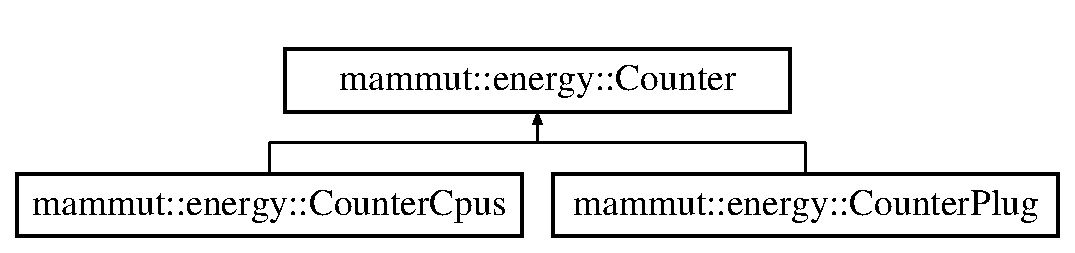
\includegraphics[height=2.000000cm]{classmammut_1_1energy_1_1Counter}
\end{center}
\end{figure}
\subsection*{Public Member Functions}
\begin{DoxyCompactItemize}
\item 
virtual Joules \hyperlink{classmammut_1_1energy_1_1Counter_a96b08f6fb969940cc5f5ee294b3b2a4a}{get\-Joules} ()=0
\item 
virtual void \hyperlink{classmammut_1_1energy_1_1Counter_aa31fb6f9fa1139a2fe3c41019801cefe}{reset} ()=0
\item 
virtual bool \hyperlink{classmammut_1_1energy_1_1Counter_abd57eea0488bd5ff8377af9ea6add7f2}{init} ()=0
\item 
virtual Counter\-Type \hyperlink{classmammut_1_1energy_1_1Counter_a6787edd9de68d900b937656a0899a954}{get\-Type} ()=0
\end{DoxyCompactItemize}


\subsection{Member Function Documentation}
\hypertarget{classmammut_1_1energy_1_1Counter_a96b08f6fb969940cc5f5ee294b3b2a4a}{\index{mammut\-::energy\-::\-Counter@{mammut\-::energy\-::\-Counter}!get\-Joules@{get\-Joules}}
\index{get\-Joules@{get\-Joules}!mammut::energy::Counter@{mammut\-::energy\-::\-Counter}}
\subsubsection[{get\-Joules}]{\setlength{\rightskip}{0pt plus 5cm}virtual Joules mammut\-::energy\-::\-Counter\-::get\-Joules (
\begin{DoxyParamCaption}
{}
\end{DoxyParamCaption}
)\hspace{0.3cm}{\ttfamily [pure virtual]}}}\label{classmammut_1_1energy_1_1Counter_a96b08f6fb969940cc5f5ee294b3b2a4a}
Returns the joules consumed up to this moment. \begin{DoxyReturn}{Returns}
The joules consumed up to this moment. 
\end{DoxyReturn}


Implemented in \hyperlink{classmammut_1_1energy_1_1CounterCpus_a6f6471724522433e88f07d60456671e5}{mammut\-::energy\-::\-Counter\-Cpus}, and \hyperlink{classmammut_1_1energy_1_1CounterPlug_a8ec0fc2cfe74fe23a0111493eac46be1}{mammut\-::energy\-::\-Counter\-Plug}.

\hypertarget{classmammut_1_1energy_1_1Counter_a6787edd9de68d900b937656a0899a954}{\index{mammut\-::energy\-::\-Counter@{mammut\-::energy\-::\-Counter}!get\-Type@{get\-Type}}
\index{get\-Type@{get\-Type}!mammut::energy::Counter@{mammut\-::energy\-::\-Counter}}
\subsubsection[{get\-Type}]{\setlength{\rightskip}{0pt plus 5cm}virtual Counter\-Type mammut\-::energy\-::\-Counter\-::get\-Type (
\begin{DoxyParamCaption}
{}
\end{DoxyParamCaption}
)\hspace{0.3cm}{\ttfamily [pure virtual]}}}\label{classmammut_1_1energy_1_1Counter_a6787edd9de68d900b937656a0899a954}
Returns the type of this counter. \begin{DoxyReturn}{Returns}
The type of this counter. 
\end{DoxyReturn}


Implemented in \hyperlink{classmammut_1_1energy_1_1CounterCpus_ad84d1173e2629965b2e2bcc823e028b7}{mammut\-::energy\-::\-Counter\-Cpus}, and \hyperlink{classmammut_1_1energy_1_1CounterPlug_a1622556a5778ac5348b48cae705bd1d9}{mammut\-::energy\-::\-Counter\-Plug}.

\hypertarget{classmammut_1_1energy_1_1Counter_abd57eea0488bd5ff8377af9ea6add7f2}{\index{mammut\-::energy\-::\-Counter@{mammut\-::energy\-::\-Counter}!init@{init}}
\index{init@{init}!mammut::energy::Counter@{mammut\-::energy\-::\-Counter}}
\subsubsection[{init}]{\setlength{\rightskip}{0pt plus 5cm}virtual bool mammut\-::energy\-::\-Counter\-::init (
\begin{DoxyParamCaption}
{}
\end{DoxyParamCaption}
)\hspace{0.3cm}{\ttfamily [pure virtual]}}}\label{classmammut_1_1energy_1_1Counter_abd57eea0488bd5ff8377af9ea6add7f2}
Initializes the counter. \begin{DoxyReturn}{Returns}
True if the counter is present, false otherwise. 
\end{DoxyReturn}


Implemented in \hyperlink{classmammut_1_1energy_1_1CounterCpus_af4496166c7b79cd60fe57baa4b6e72a1}{mammut\-::energy\-::\-Counter\-Cpus}, and \hyperlink{classmammut_1_1energy_1_1CounterPlug_ac1bbf21f8936e19e5d5380e45cbc604b}{mammut\-::energy\-::\-Counter\-Plug}.

\hypertarget{classmammut_1_1energy_1_1Counter_aa31fb6f9fa1139a2fe3c41019801cefe}{\index{mammut\-::energy\-::\-Counter@{mammut\-::energy\-::\-Counter}!reset@{reset}}
\index{reset@{reset}!mammut::energy::Counter@{mammut\-::energy\-::\-Counter}}
\subsubsection[{reset}]{\setlength{\rightskip}{0pt plus 5cm}virtual void mammut\-::energy\-::\-Counter\-::reset (
\begin{DoxyParamCaption}
{}
\end{DoxyParamCaption}
)\hspace{0.3cm}{\ttfamily [pure virtual]}}}\label{classmammut_1_1energy_1_1Counter_aa31fb6f9fa1139a2fe3c41019801cefe}
Resets the value of the counter. 

Implemented in \hyperlink{classmammut_1_1energy_1_1CounterCpus_ac3d2b3c06119c5e4f077b05689b2374a}{mammut\-::energy\-::\-Counter\-Cpus}, and \hyperlink{classmammut_1_1energy_1_1CounterPlug_af4ad1d14e69381f29ab53e1f5563eb1c}{mammut\-::energy\-::\-Counter\-Plug}.



The documentation for this class was generated from the following file\-:\begin{DoxyCompactItemize}
\item 
/home/daniele/\-Code/\-Mammut/mammut/energy/energy.\-hpp\end{DoxyCompactItemize}

\hypertarget{classmammut_1_1energy_1_1CounterCpus}{\section{mammut\-:\-:energy\-:\-:Counter\-Cpus Class Reference}
\label{classmammut_1_1energy_1_1CounterCpus}\index{mammut\-::energy\-::\-Counter\-Cpus@{mammut\-::energy\-::\-Counter\-Cpus}}
}
Inheritance diagram for mammut\-:\-:energy\-:\-:Counter\-Cpus\-:\begin{figure}[H]
\begin{center}
\leavevmode
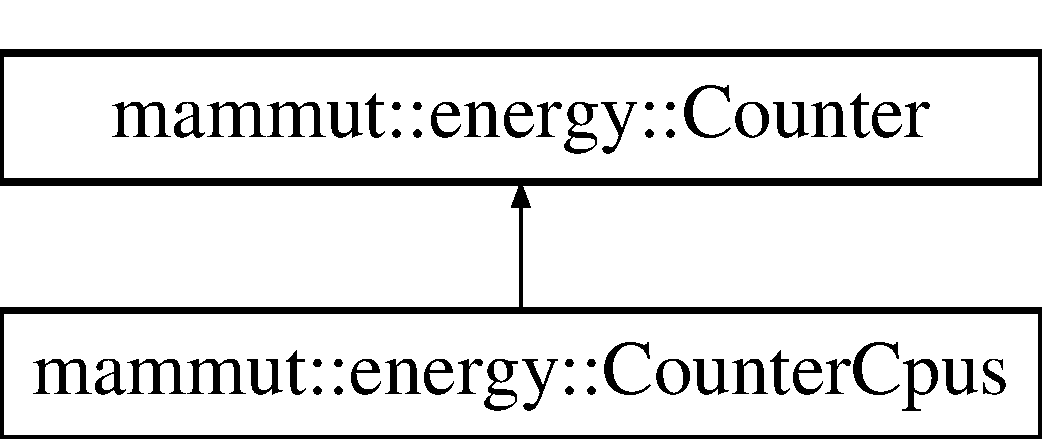
\includegraphics[height=3.000000cm]{classmammut_1_1energy_1_1CounterCpus}
\end{center}
\end{figure}
\subsection*{Public Member Functions}
\begin{DoxyCompactItemize}
\item 
const std\-::vector\\*
$<$ \hyperlink{classmammut_1_1topology_1_1Cpu}{topology\-::\-Cpu} $\ast$ $>$ \& \hyperlink{classmammut_1_1energy_1_1CounterCpus_a25dbf6940e615a3662cbe10292ad7eaa}{get\-Cpus} ()
\item 
virtual \hyperlink{classmammut_1_1energy_1_1JoulesCpu}{Joules\-Cpu} \hyperlink{classmammut_1_1energy_1_1CounterCpus_a4324fc4985dc89228450436db46551b7}{get\-Joules\-Components} (topology\-::\-Cpu\-Id cpu\-Id)=0
\item 
virtual \hyperlink{classmammut_1_1energy_1_1JoulesCpu}{Joules\-Cpu} \hyperlink{classmammut_1_1energy_1_1CounterCpus_ad6a20ef6baa36b01f55b2065e01ec3f8}{get\-Joules\-Components\-All} ()
\item 
virtual Joules \hyperlink{classmammut_1_1energy_1_1CounterCpus_a80c1f90abccce3f3ab621f08f7141f78}{get\-Joules\-Cpu} (topology\-::\-Cpu\-Id cpu\-Id)=0
\item 
virtual Joules \hyperlink{classmammut_1_1energy_1_1CounterCpus_aa50b03617eafb90d64460941a8641a28}{get\-Joules\-Cpu\-All} ()
\item 
virtual Joules \hyperlink{classmammut_1_1energy_1_1CounterCpus_a2c041bbe181f593a50490a53a2729989}{get\-Joules\-Cores} (topology\-::\-Cpu\-Id cpu\-Id)=0
\item 
virtual Joules \hyperlink{classmammut_1_1energy_1_1CounterCpus_a615edc6a1ece84d27ca1a508ec1a72d8}{get\-Joules\-Cores\-All} ()
\item 
virtual bool \hyperlink{classmammut_1_1energy_1_1CounterCpus_a94de30741049ba2131bcac532b8e7c8e}{has\-Joules\-Graphic} ()=0
\item 
virtual Joules \hyperlink{classmammut_1_1energy_1_1CounterCpus_a436f91199f40af85ce1b561781f24459}{get\-Joules\-Graphic} (topology\-::\-Cpu\-Id cpu\-Id)=0
\item 
virtual Joules \hyperlink{classmammut_1_1energy_1_1CounterCpus_a197fb5668718742b559a2c0905395359}{get\-Joules\-Graphic\-All} ()
\item 
virtual bool \hyperlink{classmammut_1_1energy_1_1CounterCpus_a3d8c64aac5808275abdb2b01a31cbc11}{has\-Joules\-Dram} ()=0
\item 
virtual Joules \hyperlink{classmammut_1_1energy_1_1CounterCpus_a832e466d0a1f40f347d9a0211059a762}{get\-Joules\-Dram} (topology\-::\-Cpu\-Id cpu\-Id)=0
\item 
virtual Joules \hyperlink{classmammut_1_1energy_1_1CounterCpus_acaadefab12684f3674f3a801d918573d}{get\-Joules\-Dram\-All} ()
\item 
Joules \hyperlink{classmammut_1_1energy_1_1CounterCpus_a6f6471724522433e88f07d60456671e5}{get\-Joules} ()
\item 
virtual void \hyperlink{classmammut_1_1energy_1_1CounterCpus_ac3d2b3c06119c5e4f077b05689b2374a}{reset} ()=0
\item 
virtual bool \hyperlink{classmammut_1_1energy_1_1CounterCpus_af4496166c7b79cd60fe57baa4b6e72a1}{init} ()=0
\item 
Counter\-Type \hyperlink{classmammut_1_1energy_1_1CounterCpus_ad84d1173e2629965b2e2bcc823e028b7}{get\-Type} ()
\end{DoxyCompactItemize}
\subsection*{Protected Member Functions}
\begin{DoxyCompactItemize}
\item 
\hypertarget{classmammut_1_1energy_1_1CounterCpus_a0a27e24202f786849a1dc5b2aaec97f9}{{\bfseries Counter\-Cpus} (\hyperlink{classmammut_1_1topology_1_1Topology}{topology\-::\-Topology} $\ast$topology)}\label{classmammut_1_1energy_1_1CounterCpus_a0a27e24202f786849a1dc5b2aaec97f9}

\end{DoxyCompactItemize}
\subsection*{Protected Attributes}
\begin{DoxyCompactItemize}
\item 
\hypertarget{classmammut_1_1energy_1_1CounterCpus_a8bf39ebc967a0b2ba256e34eeb7694e6}{\hyperlink{classmammut_1_1topology_1_1Topology}{topology\-::\-Topology} $\ast$ {\bfseries \-\_\-topology}}\label{classmammut_1_1energy_1_1CounterCpus_a8bf39ebc967a0b2ba256e34eeb7694e6}

\item 
\hypertarget{classmammut_1_1energy_1_1CounterCpus_a8af8ffffde962f5087f7aa23b3794c53}{std\-::vector$<$ \hyperlink{classmammut_1_1topology_1_1Cpu}{topology\-::\-Cpu} $\ast$ $>$ {\bfseries \-\_\-cpus}}\label{classmammut_1_1energy_1_1CounterCpus_a8af8ffffde962f5087f7aa23b3794c53}

\end{DoxyCompactItemize}


\subsection{Member Function Documentation}
\hypertarget{classmammut_1_1energy_1_1CounterCpus_a25dbf6940e615a3662cbe10292ad7eaa}{\index{mammut\-::energy\-::\-Counter\-Cpus@{mammut\-::energy\-::\-Counter\-Cpus}!get\-Cpus@{get\-Cpus}}
\index{get\-Cpus@{get\-Cpus}!mammut::energy::CounterCpus@{mammut\-::energy\-::\-Counter\-Cpus}}
\subsubsection[{get\-Cpus}]{\setlength{\rightskip}{0pt plus 5cm}const std\-::vector$<${\bf topology\-::\-Cpu}$\ast$$>$\& mammut\-::energy\-::\-Counter\-Cpus\-::get\-Cpus (
\begin{DoxyParamCaption}
{}
\end{DoxyParamCaption}
)\hspace{0.3cm}{\ttfamily [inline]}}}\label{classmammut_1_1energy_1_1CounterCpus_a25dbf6940e615a3662cbe10292ad7eaa}
Returns the Cpus. \begin{DoxyReturn}{Returns}
The Cpus. 
\end{DoxyReturn}
\hypertarget{classmammut_1_1energy_1_1CounterCpus_a6f6471724522433e88f07d60456671e5}{\index{mammut\-::energy\-::\-Counter\-Cpus@{mammut\-::energy\-::\-Counter\-Cpus}!get\-Joules@{get\-Joules}}
\index{get\-Joules@{get\-Joules}!mammut::energy::CounterCpus@{mammut\-::energy\-::\-Counter\-Cpus}}
\subsubsection[{get\-Joules}]{\setlength{\rightskip}{0pt plus 5cm}Joules mammut\-::energy\-::\-Counter\-Cpus\-::get\-Joules (
\begin{DoxyParamCaption}
{}
\end{DoxyParamCaption}
)\hspace{0.3cm}{\ttfamily [virtual]}}}\label{classmammut_1_1energy_1_1CounterCpus_a6f6471724522433e88f07d60456671e5}
Returns the joules consumed up to this moment. \begin{DoxyReturn}{Returns}
The joules consumed up to this moment. 
\end{DoxyReturn}


Implements \hyperlink{classmammut_1_1energy_1_1Counter_a96b08f6fb969940cc5f5ee294b3b2a4a}{mammut\-::energy\-::\-Counter}.

\hypertarget{classmammut_1_1energy_1_1CounterCpus_a4324fc4985dc89228450436db46551b7}{\index{mammut\-::energy\-::\-Counter\-Cpus@{mammut\-::energy\-::\-Counter\-Cpus}!get\-Joules\-Components@{get\-Joules\-Components}}
\index{get\-Joules\-Components@{get\-Joules\-Components}!mammut::energy::CounterCpus@{mammut\-::energy\-::\-Counter\-Cpus}}
\subsubsection[{get\-Joules\-Components}]{\setlength{\rightskip}{0pt plus 5cm}virtual {\bf Joules\-Cpu} mammut\-::energy\-::\-Counter\-Cpus\-::get\-Joules\-Components (
\begin{DoxyParamCaption}
\item[{topology\-::\-Cpu\-Id}]{cpu\-Id}
\end{DoxyParamCaption}
)\hspace{0.3cm}{\ttfamily [pure virtual]}}}\label{classmammut_1_1energy_1_1CounterCpus_a4324fc4985dc89228450436db46551b7}
Returns the Joules consumed by a Cpu and its components since the counter creation (or since the last call of \hyperlink{classmammut_1_1energy_1_1CounterCpus_ac3d2b3c06119c5e4f077b05689b2374a}{reset()}). 
\begin{DoxyParams}{Parameters}
{\em cpu\-Id} & The identifier of a Cpu. \\
\hline
\end{DoxyParams}
\begin{DoxyReturn}{Returns}
The Joules consumed by a Cpu and its components since the counter creation (or since the last call of \hyperlink{classmammut_1_1energy_1_1CounterCpus_ac3d2b3c06119c5e4f077b05689b2374a}{reset()}). 
\end{DoxyReturn}


Implemented in \hyperlink{classmammut_1_1energy_1_1CounterCpusLinux_a9a606911b9f9e31ef5a03225359f099f}{mammut\-::energy\-::\-Counter\-Cpus\-Linux}, and \hyperlink{classmammut_1_1energy_1_1CounterCpusRemote_a01ade74cb22a24f39d294257d764fbf3}{mammut\-::energy\-::\-Counter\-Cpus\-Remote}.

\hypertarget{classmammut_1_1energy_1_1CounterCpus_ad6a20ef6baa36b01f55b2065e01ec3f8}{\index{mammut\-::energy\-::\-Counter\-Cpus@{mammut\-::energy\-::\-Counter\-Cpus}!get\-Joules\-Components\-All@{get\-Joules\-Components\-All}}
\index{get\-Joules\-Components\-All@{get\-Joules\-Components\-All}!mammut::energy::CounterCpus@{mammut\-::energy\-::\-Counter\-Cpus}}
\subsubsection[{get\-Joules\-Components\-All}]{\setlength{\rightskip}{0pt plus 5cm}{\bf Joules\-Cpu} mammut\-::energy\-::\-Counter\-Cpus\-::get\-Joules\-Components\-All (
\begin{DoxyParamCaption}
{}
\end{DoxyParamCaption}
)\hspace{0.3cm}{\ttfamily [virtual]}}}\label{classmammut_1_1energy_1_1CounterCpus_ad6a20ef6baa36b01f55b2065e01ec3f8}
Returns the Joules consumed by all the Cpus and their components since the counter creation (or since the last call of \hyperlink{classmammut_1_1energy_1_1CounterCpus_ac3d2b3c06119c5e4f077b05689b2374a}{reset()}). \begin{DoxyReturn}{Returns}
The Joules consumed by all the Cpus and their components since the counter creation (or since the last call of \hyperlink{classmammut_1_1energy_1_1CounterCpus_ac3d2b3c06119c5e4f077b05689b2374a}{reset()}). 
\end{DoxyReturn}
\hypertarget{classmammut_1_1energy_1_1CounterCpus_a2c041bbe181f593a50490a53a2729989}{\index{mammut\-::energy\-::\-Counter\-Cpus@{mammut\-::energy\-::\-Counter\-Cpus}!get\-Joules\-Cores@{get\-Joules\-Cores}}
\index{get\-Joules\-Cores@{get\-Joules\-Cores}!mammut::energy::CounterCpus@{mammut\-::energy\-::\-Counter\-Cpus}}
\subsubsection[{get\-Joules\-Cores}]{\setlength{\rightskip}{0pt plus 5cm}virtual Joules mammut\-::energy\-::\-Counter\-Cpus\-::get\-Joules\-Cores (
\begin{DoxyParamCaption}
\item[{topology\-::\-Cpu\-Id}]{cpu\-Id}
\end{DoxyParamCaption}
)\hspace{0.3cm}{\ttfamily [pure virtual]}}}\label{classmammut_1_1energy_1_1CounterCpus_a2c041bbe181f593a50490a53a2729989}
Returns the Joules consumed by the cores of a Cpu since the counter creation (or since the last call of \hyperlink{classmammut_1_1energy_1_1CounterCpus_ac3d2b3c06119c5e4f077b05689b2374a}{reset()}). 
\begin{DoxyParams}{Parameters}
{\em cpu\-Id} & The identifier of a Cpu. \\
\hline
\end{DoxyParams}
\begin{DoxyReturn}{Returns}
The Joules consumed by the cores of a Cpu since the counter creation (or since the last call of \hyperlink{classmammut_1_1energy_1_1CounterCpus_ac3d2b3c06119c5e4f077b05689b2374a}{reset()}). 
\end{DoxyReturn}


Implemented in \hyperlink{classmammut_1_1energy_1_1CounterCpusLinux_a72e0df170e3275d33969fa162624bfce}{mammut\-::energy\-::\-Counter\-Cpus\-Linux}, and \hyperlink{classmammut_1_1energy_1_1CounterCpusRemote_aa6f49a650b0df6aecb1e56ffeca15bd7}{mammut\-::energy\-::\-Counter\-Cpus\-Remote}.

\hypertarget{classmammut_1_1energy_1_1CounterCpus_a615edc6a1ece84d27ca1a508ec1a72d8}{\index{mammut\-::energy\-::\-Counter\-Cpus@{mammut\-::energy\-::\-Counter\-Cpus}!get\-Joules\-Cores\-All@{get\-Joules\-Cores\-All}}
\index{get\-Joules\-Cores\-All@{get\-Joules\-Cores\-All}!mammut::energy::CounterCpus@{mammut\-::energy\-::\-Counter\-Cpus}}
\subsubsection[{get\-Joules\-Cores\-All}]{\setlength{\rightskip}{0pt plus 5cm}Joules mammut\-::energy\-::\-Counter\-Cpus\-::get\-Joules\-Cores\-All (
\begin{DoxyParamCaption}
{}
\end{DoxyParamCaption}
)\hspace{0.3cm}{\ttfamily [virtual]}}}\label{classmammut_1_1energy_1_1CounterCpus_a615edc6a1ece84d27ca1a508ec1a72d8}
Returns the Joules consumed by the cores of all the Cpus since the counter creation (or since the last call of \hyperlink{classmammut_1_1energy_1_1CounterCpus_ac3d2b3c06119c5e4f077b05689b2374a}{reset()}). \begin{DoxyReturn}{Returns}
The Joules consumed by the cores of all the Cpus since the counter creation (or since the last call of \hyperlink{classmammut_1_1energy_1_1CounterCpus_ac3d2b3c06119c5e4f077b05689b2374a}{reset()}). 
\end{DoxyReturn}
\hypertarget{classmammut_1_1energy_1_1CounterCpus_a80c1f90abccce3f3ab621f08f7141f78}{\index{mammut\-::energy\-::\-Counter\-Cpus@{mammut\-::energy\-::\-Counter\-Cpus}!get\-Joules\-Cpu@{get\-Joules\-Cpu}}
\index{get\-Joules\-Cpu@{get\-Joules\-Cpu}!mammut::energy::CounterCpus@{mammut\-::energy\-::\-Counter\-Cpus}}
\subsubsection[{get\-Joules\-Cpu}]{\setlength{\rightskip}{0pt plus 5cm}virtual Joules mammut\-::energy\-::\-Counter\-Cpus\-::get\-Joules\-Cpu (
\begin{DoxyParamCaption}
\item[{topology\-::\-Cpu\-Id}]{cpu\-Id}
\end{DoxyParamCaption}
)\hspace{0.3cm}{\ttfamily [pure virtual]}}}\label{classmammut_1_1energy_1_1CounterCpus_a80c1f90abccce3f3ab621f08f7141f78}
Returns the Joules consumed by a Cpu since the counter creation (or since the last call of \hyperlink{classmammut_1_1energy_1_1CounterCpus_ac3d2b3c06119c5e4f077b05689b2374a}{reset()}). 
\begin{DoxyParams}{Parameters}
{\em cpu\-Id} & The identifier of a Cpu. \\
\hline
\end{DoxyParams}
\begin{DoxyReturn}{Returns}
The Joules consumed by a Cpu since the counter creation (or since the last call of \hyperlink{classmammut_1_1energy_1_1CounterCpus_ac3d2b3c06119c5e4f077b05689b2374a}{reset()}). 
\end{DoxyReturn}


Implemented in \hyperlink{classmammut_1_1energy_1_1CounterCpusLinux_a0d02d3433187bdc382ca4f5aa14f17fe}{mammut\-::energy\-::\-Counter\-Cpus\-Linux}, and \hyperlink{classmammut_1_1energy_1_1CounterCpusRemote_a1c55fc9f3bbcaed7d16e526175eca00c}{mammut\-::energy\-::\-Counter\-Cpus\-Remote}.

\hypertarget{classmammut_1_1energy_1_1CounterCpus_aa50b03617eafb90d64460941a8641a28}{\index{mammut\-::energy\-::\-Counter\-Cpus@{mammut\-::energy\-::\-Counter\-Cpus}!get\-Joules\-Cpu\-All@{get\-Joules\-Cpu\-All}}
\index{get\-Joules\-Cpu\-All@{get\-Joules\-Cpu\-All}!mammut::energy::CounterCpus@{mammut\-::energy\-::\-Counter\-Cpus}}
\subsubsection[{get\-Joules\-Cpu\-All}]{\setlength{\rightskip}{0pt plus 5cm}Joules mammut\-::energy\-::\-Counter\-Cpus\-::get\-Joules\-Cpu\-All (
\begin{DoxyParamCaption}
{}
\end{DoxyParamCaption}
)\hspace{0.3cm}{\ttfamily [virtual]}}}\label{classmammut_1_1energy_1_1CounterCpus_aa50b03617eafb90d64460941a8641a28}
Returns the Joules consumed by all the Cpus since the counter creation (or since the last call of \hyperlink{classmammut_1_1energy_1_1CounterCpus_ac3d2b3c06119c5e4f077b05689b2374a}{reset()}). \begin{DoxyReturn}{Returns}
The Joules consumed by all the Cpus since the counter creation (or since the last call of \hyperlink{classmammut_1_1energy_1_1CounterCpus_ac3d2b3c06119c5e4f077b05689b2374a}{reset()}). 
\end{DoxyReturn}
\hypertarget{classmammut_1_1energy_1_1CounterCpus_a832e466d0a1f40f347d9a0211059a762}{\index{mammut\-::energy\-::\-Counter\-Cpus@{mammut\-::energy\-::\-Counter\-Cpus}!get\-Joules\-Dram@{get\-Joules\-Dram}}
\index{get\-Joules\-Dram@{get\-Joules\-Dram}!mammut::energy::CounterCpus@{mammut\-::energy\-::\-Counter\-Cpus}}
\subsubsection[{get\-Joules\-Dram}]{\setlength{\rightskip}{0pt plus 5cm}virtual Joules mammut\-::energy\-::\-Counter\-Cpus\-::get\-Joules\-Dram (
\begin{DoxyParamCaption}
\item[{topology\-::\-Cpu\-Id}]{cpu\-Id}
\end{DoxyParamCaption}
)\hspace{0.3cm}{\ttfamily [pure virtual]}}}\label{classmammut_1_1energy_1_1CounterCpus_a832e466d0a1f40f347d9a0211059a762}
Returns the Joules consumed by a Cpu Dram since the counter creation (or since the last call of \hyperlink{classmammut_1_1energy_1_1CounterCpus_ac3d2b3c06119c5e4f077b05689b2374a}{reset()}). 
\begin{DoxyParams}{Parameters}
{\em cpu\-Id} & The identifier of a Cpu. \\
\hline
\end{DoxyParams}
\begin{DoxyReturn}{Returns}
The Joules consumed by a Cpu Dram since the counter creation (or since the last call of \hyperlink{classmammut_1_1energy_1_1CounterCpus_ac3d2b3c06119c5e4f077b05689b2374a}{reset()}). 
\end{DoxyReturn}


Implemented in \hyperlink{classmammut_1_1energy_1_1CounterCpusLinux_a444feaaad6ad295c7f70c245043fed2c}{mammut\-::energy\-::\-Counter\-Cpus\-Linux}, and \hyperlink{classmammut_1_1energy_1_1CounterCpusRemote_a95558006c8d7e8453af38ff57ce0d3ff}{mammut\-::energy\-::\-Counter\-Cpus\-Remote}.

\hypertarget{classmammut_1_1energy_1_1CounterCpus_acaadefab12684f3674f3a801d918573d}{\index{mammut\-::energy\-::\-Counter\-Cpus@{mammut\-::energy\-::\-Counter\-Cpus}!get\-Joules\-Dram\-All@{get\-Joules\-Dram\-All}}
\index{get\-Joules\-Dram\-All@{get\-Joules\-Dram\-All}!mammut::energy::CounterCpus@{mammut\-::energy\-::\-Counter\-Cpus}}
\subsubsection[{get\-Joules\-Dram\-All}]{\setlength{\rightskip}{0pt plus 5cm}Joules mammut\-::energy\-::\-Counter\-Cpus\-::get\-Joules\-Dram\-All (
\begin{DoxyParamCaption}
{}
\end{DoxyParamCaption}
)\hspace{0.3cm}{\ttfamily [virtual]}}}\label{classmammut_1_1energy_1_1CounterCpus_acaadefab12684f3674f3a801d918573d}
Returns the Joules consumed by all the Cpus Dram since the counter creation (or since the last call of \hyperlink{classmammut_1_1energy_1_1CounterCpus_ac3d2b3c06119c5e4f077b05689b2374a}{reset()}). \begin{DoxyReturn}{Returns}
The Joules consumed by all the Cpus Dram since the counter creation (or since the last call of \hyperlink{classmammut_1_1energy_1_1CounterCpus_ac3d2b3c06119c5e4f077b05689b2374a}{reset()}). 
\end{DoxyReturn}
\hypertarget{classmammut_1_1energy_1_1CounterCpus_a436f91199f40af85ce1b561781f24459}{\index{mammut\-::energy\-::\-Counter\-Cpus@{mammut\-::energy\-::\-Counter\-Cpus}!get\-Joules\-Graphic@{get\-Joules\-Graphic}}
\index{get\-Joules\-Graphic@{get\-Joules\-Graphic}!mammut::energy::CounterCpus@{mammut\-::energy\-::\-Counter\-Cpus}}
\subsubsection[{get\-Joules\-Graphic}]{\setlength{\rightskip}{0pt plus 5cm}virtual Joules mammut\-::energy\-::\-Counter\-Cpus\-::get\-Joules\-Graphic (
\begin{DoxyParamCaption}
\item[{topology\-::\-Cpu\-Id}]{cpu\-Id}
\end{DoxyParamCaption}
)\hspace{0.3cm}{\ttfamily [pure virtual]}}}\label{classmammut_1_1energy_1_1CounterCpus_a436f91199f40af85ce1b561781f24459}
Returns the Joules consumed by a Cpu integrated graphic card (if present) since the counter creation (or since the last call of \hyperlink{classmammut_1_1energy_1_1CounterCpus_ac3d2b3c06119c5e4f077b05689b2374a}{reset()}). 
\begin{DoxyParams}{Parameters}
{\em cpu\-Id} & The identifier of a Cpu. \\
\hline
\end{DoxyParams}
\begin{DoxyReturn}{Returns}
The Joules consumed by a Cpu integrated graphic card (if present) since the counter creation (or since the last call of \hyperlink{classmammut_1_1energy_1_1CounterCpus_ac3d2b3c06119c5e4f077b05689b2374a}{reset()}). 
\end{DoxyReturn}


Implemented in \hyperlink{classmammut_1_1energy_1_1CounterCpusLinux_ad8dc0f2a9618e6d013b45090a7060042}{mammut\-::energy\-::\-Counter\-Cpus\-Linux}, and \hyperlink{classmammut_1_1energy_1_1CounterCpusRemote_af886a7df65acafc4bb762fb45a91bfaa}{mammut\-::energy\-::\-Counter\-Cpus\-Remote}.

\hypertarget{classmammut_1_1energy_1_1CounterCpus_a197fb5668718742b559a2c0905395359}{\index{mammut\-::energy\-::\-Counter\-Cpus@{mammut\-::energy\-::\-Counter\-Cpus}!get\-Joules\-Graphic\-All@{get\-Joules\-Graphic\-All}}
\index{get\-Joules\-Graphic\-All@{get\-Joules\-Graphic\-All}!mammut::energy::CounterCpus@{mammut\-::energy\-::\-Counter\-Cpus}}
\subsubsection[{get\-Joules\-Graphic\-All}]{\setlength{\rightskip}{0pt plus 5cm}Joules mammut\-::energy\-::\-Counter\-Cpus\-::get\-Joules\-Graphic\-All (
\begin{DoxyParamCaption}
{}
\end{DoxyParamCaption}
)\hspace{0.3cm}{\ttfamily [virtual]}}}\label{classmammut_1_1energy_1_1CounterCpus_a197fb5668718742b559a2c0905395359}
Returns the Joules consumed by all the Cpus integrated graphic card (if present) since the counter creation (or since the last call of \hyperlink{classmammut_1_1energy_1_1CounterCpus_ac3d2b3c06119c5e4f077b05689b2374a}{reset()}). \begin{DoxyReturn}{Returns}
The Joules consumed by all the Cpus integrated graphic card (if present) since the counter creation (or since the last call of \hyperlink{classmammut_1_1energy_1_1CounterCpus_ac3d2b3c06119c5e4f077b05689b2374a}{reset()}). 
\end{DoxyReturn}
\hypertarget{classmammut_1_1energy_1_1CounterCpus_ad84d1173e2629965b2e2bcc823e028b7}{\index{mammut\-::energy\-::\-Counter\-Cpus@{mammut\-::energy\-::\-Counter\-Cpus}!get\-Type@{get\-Type}}
\index{get\-Type@{get\-Type}!mammut::energy::CounterCpus@{mammut\-::energy\-::\-Counter\-Cpus}}
\subsubsection[{get\-Type}]{\setlength{\rightskip}{0pt plus 5cm}Counter\-Type mammut\-::energy\-::\-Counter\-Cpus\-::get\-Type (
\begin{DoxyParamCaption}
{}
\end{DoxyParamCaption}
)\hspace{0.3cm}{\ttfamily [inline]}, {\ttfamily [virtual]}}}\label{classmammut_1_1energy_1_1CounterCpus_ad84d1173e2629965b2e2bcc823e028b7}
Returns the type of this counter. \begin{DoxyReturn}{Returns}
The type of this counter. 
\end{DoxyReturn}


Implements \hyperlink{classmammut_1_1energy_1_1Counter_a6787edd9de68d900b937656a0899a954}{mammut\-::energy\-::\-Counter}.

\hypertarget{classmammut_1_1energy_1_1CounterCpus_a3d8c64aac5808275abdb2b01a31cbc11}{\index{mammut\-::energy\-::\-Counter\-Cpus@{mammut\-::energy\-::\-Counter\-Cpus}!has\-Joules\-Dram@{has\-Joules\-Dram}}
\index{has\-Joules\-Dram@{has\-Joules\-Dram}!mammut::energy::CounterCpus@{mammut\-::energy\-::\-Counter\-Cpus}}
\subsubsection[{has\-Joules\-Dram}]{\setlength{\rightskip}{0pt plus 5cm}virtual bool mammut\-::energy\-::\-Counter\-Cpus\-::has\-Joules\-Dram (
\begin{DoxyParamCaption}
{}
\end{DoxyParamCaption}
)\hspace{0.3cm}{\ttfamily [pure virtual]}}}\label{classmammut_1_1energy_1_1CounterCpus_a3d8c64aac5808275abdb2b01a31cbc11}
Returns true if the counter for D\-R\-A\-M is present, false otherwise. \begin{DoxyReturn}{Returns}
True if the counter for D\-R\-A\-M is present, false otherwise. 
\end{DoxyReturn}


Implemented in \hyperlink{classmammut_1_1energy_1_1CounterCpusLinux_a8fcb24f3bdb1a66338ff3fdbbba9ec6b}{mammut\-::energy\-::\-Counter\-Cpus\-Linux}, and \hyperlink{classmammut_1_1energy_1_1CounterCpusRemote_a7e50db0df2b842a7596e5ec559f477bf}{mammut\-::energy\-::\-Counter\-Cpus\-Remote}.

\hypertarget{classmammut_1_1energy_1_1CounterCpus_a94de30741049ba2131bcac532b8e7c8e}{\index{mammut\-::energy\-::\-Counter\-Cpus@{mammut\-::energy\-::\-Counter\-Cpus}!has\-Joules\-Graphic@{has\-Joules\-Graphic}}
\index{has\-Joules\-Graphic@{has\-Joules\-Graphic}!mammut::energy::CounterCpus@{mammut\-::energy\-::\-Counter\-Cpus}}
\subsubsection[{has\-Joules\-Graphic}]{\setlength{\rightskip}{0pt plus 5cm}virtual bool mammut\-::energy\-::\-Counter\-Cpus\-::has\-Joules\-Graphic (
\begin{DoxyParamCaption}
{}
\end{DoxyParamCaption}
)\hspace{0.3cm}{\ttfamily [pure virtual]}}}\label{classmammut_1_1energy_1_1CounterCpus_a94de30741049ba2131bcac532b8e7c8e}
Returns true if the counter for integrated graphic card is present, false otherwise. \begin{DoxyReturn}{Returns}
True if the counter for integrated graphic card is present, false otherwise. 
\end{DoxyReturn}


Implemented in \hyperlink{classmammut_1_1energy_1_1CounterCpusLinux_a2390a3c17505d5e87490a6b50831c426}{mammut\-::energy\-::\-Counter\-Cpus\-Linux}, and \hyperlink{classmammut_1_1energy_1_1CounterCpusRemote_a315765ac4950dee79408301db828a834}{mammut\-::energy\-::\-Counter\-Cpus\-Remote}.

\hypertarget{classmammut_1_1energy_1_1CounterCpus_af4496166c7b79cd60fe57baa4b6e72a1}{\index{mammut\-::energy\-::\-Counter\-Cpus@{mammut\-::energy\-::\-Counter\-Cpus}!init@{init}}
\index{init@{init}!mammut::energy::CounterCpus@{mammut\-::energy\-::\-Counter\-Cpus}}
\subsubsection[{init}]{\setlength{\rightskip}{0pt plus 5cm}virtual bool mammut\-::energy\-::\-Counter\-Cpus\-::init (
\begin{DoxyParamCaption}
{}
\end{DoxyParamCaption}
)\hspace{0.3cm}{\ttfamily [pure virtual]}}}\label{classmammut_1_1energy_1_1CounterCpus_af4496166c7b79cd60fe57baa4b6e72a1}
Initializes the counter. \begin{DoxyReturn}{Returns}
True if the counter is present, false otherwise. 
\end{DoxyReturn}


Implements \hyperlink{classmammut_1_1energy_1_1Counter_abd57eea0488bd5ff8377af9ea6add7f2}{mammut\-::energy\-::\-Counter}.



Implemented in \hyperlink{classmammut_1_1energy_1_1CounterCpusLinux_ac7169ddb9d47da49a6251b3f1c380675}{mammut\-::energy\-::\-Counter\-Cpus\-Linux}, and \hyperlink{classmammut_1_1energy_1_1CounterCpusRemote_a68203a642d22edc316c7b95bddfa4e15}{mammut\-::energy\-::\-Counter\-Cpus\-Remote}.

\hypertarget{classmammut_1_1energy_1_1CounterCpus_ac3d2b3c06119c5e4f077b05689b2374a}{\index{mammut\-::energy\-::\-Counter\-Cpus@{mammut\-::energy\-::\-Counter\-Cpus}!reset@{reset}}
\index{reset@{reset}!mammut::energy::CounterCpus@{mammut\-::energy\-::\-Counter\-Cpus}}
\subsubsection[{reset}]{\setlength{\rightskip}{0pt plus 5cm}virtual void mammut\-::energy\-::\-Counter\-Cpus\-::reset (
\begin{DoxyParamCaption}
{}
\end{DoxyParamCaption}
)\hspace{0.3cm}{\ttfamily [pure virtual]}}}\label{classmammut_1_1energy_1_1CounterCpus_ac3d2b3c06119c5e4f077b05689b2374a}
Resets the value of the counter. 

Implements \hyperlink{classmammut_1_1energy_1_1Counter_aa31fb6f9fa1139a2fe3c41019801cefe}{mammut\-::energy\-::\-Counter}.



Implemented in \hyperlink{classmammut_1_1energy_1_1CounterCpusLinux_aa1ad68623ce7571a7570398c5488a65b}{mammut\-::energy\-::\-Counter\-Cpus\-Linux}, and \hyperlink{classmammut_1_1energy_1_1CounterCpusRemote_a20439f71fc4d024be5470cec09bd0355}{mammut\-::energy\-::\-Counter\-Cpus\-Remote}.



The documentation for this class was generated from the following files\-:\begin{DoxyCompactItemize}
\item 
/home/daniele/\-Code/\-Mammut/mammut/energy/energy.\-hpp\item 
/home/daniele/\-Code/\-Mammut/mammut/energy/energy.\-cpp\end{DoxyCompactItemize}

\hypertarget{classmammut_1_1energy_1_1CounterCpusLinux}{\section{mammut\-:\-:energy\-:\-:Counter\-Cpus\-Linux Class Reference}
\label{classmammut_1_1energy_1_1CounterCpusLinux}\index{mammut\-::energy\-::\-Counter\-Cpus\-Linux@{mammut\-::energy\-::\-Counter\-Cpus\-Linux}}
}
Inheritance diagram for mammut\-:\-:energy\-:\-:Counter\-Cpus\-Linux\-:\begin{figure}[H]
\begin{center}
\leavevmode
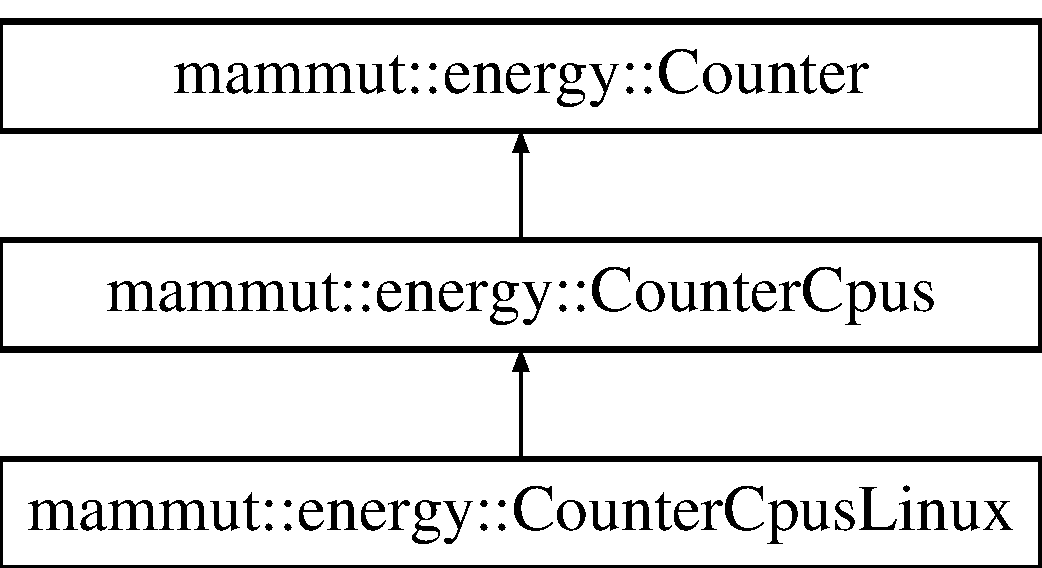
\includegraphics[height=3.000000cm]{classmammut_1_1energy_1_1CounterCpusLinux}
\end{center}
\end{figure}
\subsection*{Public Member Functions}
\begin{DoxyCompactItemize}
\item 
\hyperlink{classmammut_1_1energy_1_1JoulesCpu}{Joules\-Cpu} \hyperlink{classmammut_1_1energy_1_1CounterCpusLinux_a9a606911b9f9e31ef5a03225359f099f}{get\-Joules\-Components} (topology\-::\-Cpu\-Id cpu\-Id)
\item 
Joules \hyperlink{classmammut_1_1energy_1_1CounterCpusLinux_a0d02d3433187bdc382ca4f5aa14f17fe}{get\-Joules\-Cpu} (topology\-::\-Cpu\-Id cpu\-Id)
\item 
Joules \hyperlink{classmammut_1_1energy_1_1CounterCpusLinux_a72e0df170e3275d33969fa162624bfce}{get\-Joules\-Cores} (topology\-::\-Cpu\-Id cpu\-Id)
\item 
Joules \hyperlink{classmammut_1_1energy_1_1CounterCpusLinux_ad8dc0f2a9618e6d013b45090a7060042}{get\-Joules\-Graphic} (topology\-::\-Cpu\-Id cpu\-Id)
\item 
Joules \hyperlink{classmammut_1_1energy_1_1CounterCpusLinux_a444feaaad6ad295c7f70c245043fed2c}{get\-Joules\-Dram} (topology\-::\-Cpu\-Id cpu\-Id)
\item 
bool \hyperlink{classmammut_1_1energy_1_1CounterCpusLinux_a8fcb24f3bdb1a66338ff3fdbbba9ec6b}{has\-Joules\-Dram} ()
\item 
bool \hyperlink{classmammut_1_1energy_1_1CounterCpusLinux_a2390a3c17505d5e87490a6b50831c426}{has\-Joules\-Graphic} ()
\item 
bool \hyperlink{classmammut_1_1energy_1_1CounterCpusLinux_ac7169ddb9d47da49a6251b3f1c380675}{init} ()
\item 
void \hyperlink{classmammut_1_1energy_1_1CounterCpusLinux_aa1ad68623ce7571a7570398c5488a65b}{reset} ()
\end{DoxyCompactItemize}
\subsection*{Friends}
\begin{DoxyCompactItemize}
\item 
\hypertarget{classmammut_1_1energy_1_1CounterCpusLinux_a1fd3f6def9f7901bd7754805a29b95ea}{class {\bfseries Counter\-Cpus\-Linux\-Refresher}}\label{classmammut_1_1energy_1_1CounterCpusLinux_a1fd3f6def9f7901bd7754805a29b95ea}

\end{DoxyCompactItemize}
\subsection*{Additional Inherited Members}


\subsection{Member Function Documentation}
\hypertarget{classmammut_1_1energy_1_1CounterCpusLinux_a9a606911b9f9e31ef5a03225359f099f}{\index{mammut\-::energy\-::\-Counter\-Cpus\-Linux@{mammut\-::energy\-::\-Counter\-Cpus\-Linux}!get\-Joules\-Components@{get\-Joules\-Components}}
\index{get\-Joules\-Components@{get\-Joules\-Components}!mammut::energy::CounterCpusLinux@{mammut\-::energy\-::\-Counter\-Cpus\-Linux}}
\subsubsection[{get\-Joules\-Components}]{\setlength{\rightskip}{0pt plus 5cm}{\bf Joules\-Cpu} mammut\-::energy\-::\-Counter\-Cpus\-Linux\-::get\-Joules\-Components (
\begin{DoxyParamCaption}
\item[{topology\-::\-Cpu\-Id}]{cpu\-Id}
\end{DoxyParamCaption}
)\hspace{0.3cm}{\ttfamily [virtual]}}}\label{classmammut_1_1energy_1_1CounterCpusLinux_a9a606911b9f9e31ef5a03225359f099f}
Returns the Joules consumed by a Cpu and its components since the counter creation (or since the last call of \hyperlink{classmammut_1_1energy_1_1CounterCpusLinux_aa1ad68623ce7571a7570398c5488a65b}{reset()}). 
\begin{DoxyParams}{Parameters}
{\em cpu\-Id} & The identifier of a Cpu. \\
\hline
\end{DoxyParams}
\begin{DoxyReturn}{Returns}
The Joules consumed by a Cpu and its components since the counter creation (or since the last call of \hyperlink{classmammut_1_1energy_1_1CounterCpusLinux_aa1ad68623ce7571a7570398c5488a65b}{reset()}). 
\end{DoxyReturn}


Implements \hyperlink{classmammut_1_1energy_1_1CounterCpus_a4324fc4985dc89228450436db46551b7}{mammut\-::energy\-::\-Counter\-Cpus}.

\hypertarget{classmammut_1_1energy_1_1CounterCpusLinux_a72e0df170e3275d33969fa162624bfce}{\index{mammut\-::energy\-::\-Counter\-Cpus\-Linux@{mammut\-::energy\-::\-Counter\-Cpus\-Linux}!get\-Joules\-Cores@{get\-Joules\-Cores}}
\index{get\-Joules\-Cores@{get\-Joules\-Cores}!mammut::energy::CounterCpusLinux@{mammut\-::energy\-::\-Counter\-Cpus\-Linux}}
\subsubsection[{get\-Joules\-Cores}]{\setlength{\rightskip}{0pt plus 5cm}Joules mammut\-::energy\-::\-Counter\-Cpus\-Linux\-::get\-Joules\-Cores (
\begin{DoxyParamCaption}
\item[{topology\-::\-Cpu\-Id}]{cpu\-Id}
\end{DoxyParamCaption}
)\hspace{0.3cm}{\ttfamily [virtual]}}}\label{classmammut_1_1energy_1_1CounterCpusLinux_a72e0df170e3275d33969fa162624bfce}
Returns the Joules consumed by the cores of a Cpu since the counter creation (or since the last call of \hyperlink{classmammut_1_1energy_1_1CounterCpusLinux_aa1ad68623ce7571a7570398c5488a65b}{reset()}). 
\begin{DoxyParams}{Parameters}
{\em cpu\-Id} & The identifier of a Cpu. \\
\hline
\end{DoxyParams}
\begin{DoxyReturn}{Returns}
The Joules consumed by the cores of a Cpu since the counter creation (or since the last call of \hyperlink{classmammut_1_1energy_1_1CounterCpusLinux_aa1ad68623ce7571a7570398c5488a65b}{reset()}). 
\end{DoxyReturn}


Implements \hyperlink{classmammut_1_1energy_1_1CounterCpus_a2c041bbe181f593a50490a53a2729989}{mammut\-::energy\-::\-Counter\-Cpus}.

\hypertarget{classmammut_1_1energy_1_1CounterCpusLinux_a0d02d3433187bdc382ca4f5aa14f17fe}{\index{mammut\-::energy\-::\-Counter\-Cpus\-Linux@{mammut\-::energy\-::\-Counter\-Cpus\-Linux}!get\-Joules\-Cpu@{get\-Joules\-Cpu}}
\index{get\-Joules\-Cpu@{get\-Joules\-Cpu}!mammut::energy::CounterCpusLinux@{mammut\-::energy\-::\-Counter\-Cpus\-Linux}}
\subsubsection[{get\-Joules\-Cpu}]{\setlength{\rightskip}{0pt plus 5cm}Joules mammut\-::energy\-::\-Counter\-Cpus\-Linux\-::get\-Joules\-Cpu (
\begin{DoxyParamCaption}
\item[{topology\-::\-Cpu\-Id}]{cpu\-Id}
\end{DoxyParamCaption}
)\hspace{0.3cm}{\ttfamily [virtual]}}}\label{classmammut_1_1energy_1_1CounterCpusLinux_a0d02d3433187bdc382ca4f5aa14f17fe}
Returns the Joules consumed by a Cpu since the counter creation (or since the last call of \hyperlink{classmammut_1_1energy_1_1CounterCpusLinux_aa1ad68623ce7571a7570398c5488a65b}{reset()}). 
\begin{DoxyParams}{Parameters}
{\em cpu\-Id} & The identifier of a Cpu. \\
\hline
\end{DoxyParams}
\begin{DoxyReturn}{Returns}
The Joules consumed by a Cpu since the counter creation (or since the last call of \hyperlink{classmammut_1_1energy_1_1CounterCpusLinux_aa1ad68623ce7571a7570398c5488a65b}{reset()}). 
\end{DoxyReturn}


Implements \hyperlink{classmammut_1_1energy_1_1CounterCpus_a80c1f90abccce3f3ab621f08f7141f78}{mammut\-::energy\-::\-Counter\-Cpus}.

\hypertarget{classmammut_1_1energy_1_1CounterCpusLinux_a444feaaad6ad295c7f70c245043fed2c}{\index{mammut\-::energy\-::\-Counter\-Cpus\-Linux@{mammut\-::energy\-::\-Counter\-Cpus\-Linux}!get\-Joules\-Dram@{get\-Joules\-Dram}}
\index{get\-Joules\-Dram@{get\-Joules\-Dram}!mammut::energy::CounterCpusLinux@{mammut\-::energy\-::\-Counter\-Cpus\-Linux}}
\subsubsection[{get\-Joules\-Dram}]{\setlength{\rightskip}{0pt plus 5cm}Joules mammut\-::energy\-::\-Counter\-Cpus\-Linux\-::get\-Joules\-Dram (
\begin{DoxyParamCaption}
\item[{topology\-::\-Cpu\-Id}]{cpu\-Id}
\end{DoxyParamCaption}
)\hspace{0.3cm}{\ttfamily [virtual]}}}\label{classmammut_1_1energy_1_1CounterCpusLinux_a444feaaad6ad295c7f70c245043fed2c}
Returns the Joules consumed by a Cpu Dram since the counter creation (or since the last call of \hyperlink{classmammut_1_1energy_1_1CounterCpusLinux_aa1ad68623ce7571a7570398c5488a65b}{reset()}). 
\begin{DoxyParams}{Parameters}
{\em cpu\-Id} & The identifier of a Cpu. \\
\hline
\end{DoxyParams}
\begin{DoxyReturn}{Returns}
The Joules consumed by a Cpu Dram since the counter creation (or since the last call of \hyperlink{classmammut_1_1energy_1_1CounterCpusLinux_aa1ad68623ce7571a7570398c5488a65b}{reset()}). 
\end{DoxyReturn}


Implements \hyperlink{classmammut_1_1energy_1_1CounterCpus_a832e466d0a1f40f347d9a0211059a762}{mammut\-::energy\-::\-Counter\-Cpus}.

\hypertarget{classmammut_1_1energy_1_1CounterCpusLinux_ad8dc0f2a9618e6d013b45090a7060042}{\index{mammut\-::energy\-::\-Counter\-Cpus\-Linux@{mammut\-::energy\-::\-Counter\-Cpus\-Linux}!get\-Joules\-Graphic@{get\-Joules\-Graphic}}
\index{get\-Joules\-Graphic@{get\-Joules\-Graphic}!mammut::energy::CounterCpusLinux@{mammut\-::energy\-::\-Counter\-Cpus\-Linux}}
\subsubsection[{get\-Joules\-Graphic}]{\setlength{\rightskip}{0pt plus 5cm}Joules mammut\-::energy\-::\-Counter\-Cpus\-Linux\-::get\-Joules\-Graphic (
\begin{DoxyParamCaption}
\item[{topology\-::\-Cpu\-Id}]{cpu\-Id}
\end{DoxyParamCaption}
)\hspace{0.3cm}{\ttfamily [virtual]}}}\label{classmammut_1_1energy_1_1CounterCpusLinux_ad8dc0f2a9618e6d013b45090a7060042}
Returns the Joules consumed by a Cpu integrated graphic card (if present) since the counter creation (or since the last call of \hyperlink{classmammut_1_1energy_1_1CounterCpusLinux_aa1ad68623ce7571a7570398c5488a65b}{reset()}). 
\begin{DoxyParams}{Parameters}
{\em cpu\-Id} & The identifier of a Cpu. \\
\hline
\end{DoxyParams}
\begin{DoxyReturn}{Returns}
The Joules consumed by a Cpu integrated graphic card (if present) since the counter creation (or since the last call of \hyperlink{classmammut_1_1energy_1_1CounterCpusLinux_aa1ad68623ce7571a7570398c5488a65b}{reset()}). 
\end{DoxyReturn}


Implements \hyperlink{classmammut_1_1energy_1_1CounterCpus_a436f91199f40af85ce1b561781f24459}{mammut\-::energy\-::\-Counter\-Cpus}.

\hypertarget{classmammut_1_1energy_1_1CounterCpusLinux_a8fcb24f3bdb1a66338ff3fdbbba9ec6b}{\index{mammut\-::energy\-::\-Counter\-Cpus\-Linux@{mammut\-::energy\-::\-Counter\-Cpus\-Linux}!has\-Joules\-Dram@{has\-Joules\-Dram}}
\index{has\-Joules\-Dram@{has\-Joules\-Dram}!mammut::energy::CounterCpusLinux@{mammut\-::energy\-::\-Counter\-Cpus\-Linux}}
\subsubsection[{has\-Joules\-Dram}]{\setlength{\rightskip}{0pt plus 5cm}bool mammut\-::energy\-::\-Counter\-Cpus\-Linux\-::has\-Joules\-Dram (
\begin{DoxyParamCaption}
{}
\end{DoxyParamCaption}
)\hspace{0.3cm}{\ttfamily [virtual]}}}\label{classmammut_1_1energy_1_1CounterCpusLinux_a8fcb24f3bdb1a66338ff3fdbbba9ec6b}
Returns true if the counter for D\-R\-A\-M is present, false otherwise. \begin{DoxyReturn}{Returns}
True if the counter for D\-R\-A\-M is present, false otherwise. 
\end{DoxyReturn}


Implements \hyperlink{classmammut_1_1energy_1_1CounterCpus_a3d8c64aac5808275abdb2b01a31cbc11}{mammut\-::energy\-::\-Counter\-Cpus}.

\hypertarget{classmammut_1_1energy_1_1CounterCpusLinux_a2390a3c17505d5e87490a6b50831c426}{\index{mammut\-::energy\-::\-Counter\-Cpus\-Linux@{mammut\-::energy\-::\-Counter\-Cpus\-Linux}!has\-Joules\-Graphic@{has\-Joules\-Graphic}}
\index{has\-Joules\-Graphic@{has\-Joules\-Graphic}!mammut::energy::CounterCpusLinux@{mammut\-::energy\-::\-Counter\-Cpus\-Linux}}
\subsubsection[{has\-Joules\-Graphic}]{\setlength{\rightskip}{0pt plus 5cm}bool mammut\-::energy\-::\-Counter\-Cpus\-Linux\-::has\-Joules\-Graphic (
\begin{DoxyParamCaption}
{}
\end{DoxyParamCaption}
)\hspace{0.3cm}{\ttfamily [virtual]}}}\label{classmammut_1_1energy_1_1CounterCpusLinux_a2390a3c17505d5e87490a6b50831c426}
Returns true if the counter for integrated graphic card is present, false otherwise. \begin{DoxyReturn}{Returns}
True if the counter for integrated graphic card is present, false otherwise. 
\end{DoxyReturn}


Implements \hyperlink{classmammut_1_1energy_1_1CounterCpus_a94de30741049ba2131bcac532b8e7c8e}{mammut\-::energy\-::\-Counter\-Cpus}.

\hypertarget{classmammut_1_1energy_1_1CounterCpusLinux_ac7169ddb9d47da49a6251b3f1c380675}{\index{mammut\-::energy\-::\-Counter\-Cpus\-Linux@{mammut\-::energy\-::\-Counter\-Cpus\-Linux}!init@{init}}
\index{init@{init}!mammut::energy::CounterCpusLinux@{mammut\-::energy\-::\-Counter\-Cpus\-Linux}}
\subsubsection[{init}]{\setlength{\rightskip}{0pt plus 5cm}bool mammut\-::energy\-::\-Counter\-Cpus\-Linux\-::init (
\begin{DoxyParamCaption}
{}
\end{DoxyParamCaption}
)\hspace{0.3cm}{\ttfamily [virtual]}}}\label{classmammut_1_1energy_1_1CounterCpusLinux_ac7169ddb9d47da49a6251b3f1c380675}
Initializes the counter. \begin{DoxyReturn}{Returns}
True if the counter is present, false otherwise. 
\end{DoxyReturn}
I have one msr for each C\-P\-U. Since I have no guarantee that the C\-P\-U identifiers are contiguous, I find their maximum id to decide how long the array of msrs should be. For example, if a have a C\-P\-U with id 1 and a C\-P\-U with id 3, then I will allocate an array of 4 positions. In msrs\mbox{[}1\mbox{]} I will have the msr associated to C\-P\-U 1 and in msrs\mbox{[}3\mbox{]} I will have the msr associated to C\-P\-U 3.

Implements \hyperlink{classmammut_1_1energy_1_1CounterCpus_af4496166c7b79cd60fe57baa4b6e72a1}{mammut\-::energy\-::\-Counter\-Cpus}.

\hypertarget{classmammut_1_1energy_1_1CounterCpusLinux_aa1ad68623ce7571a7570398c5488a65b}{\index{mammut\-::energy\-::\-Counter\-Cpus\-Linux@{mammut\-::energy\-::\-Counter\-Cpus\-Linux}!reset@{reset}}
\index{reset@{reset}!mammut::energy::CounterCpusLinux@{mammut\-::energy\-::\-Counter\-Cpus\-Linux}}
\subsubsection[{reset}]{\setlength{\rightskip}{0pt plus 5cm}void mammut\-::energy\-::\-Counter\-Cpus\-Linux\-::reset (
\begin{DoxyParamCaption}
{}
\end{DoxyParamCaption}
)\hspace{0.3cm}{\ttfamily [virtual]}}}\label{classmammut_1_1energy_1_1CounterCpusLinux_aa1ad68623ce7571a7570398c5488a65b}
Resets the value of the counter. 

Implements \hyperlink{classmammut_1_1energy_1_1CounterCpus_ac3d2b3c06119c5e4f077b05689b2374a}{mammut\-::energy\-::\-Counter\-Cpus}.



The documentation for this class was generated from the following files\-:\begin{DoxyCompactItemize}
\item 
/home/daniele/\-Code/\-Mammut/mammut/energy/energy-\/linux.\-hpp\item 
/home/daniele/\-Code/\-Mammut/mammut/energy/energy-\/linux.\-cpp\end{DoxyCompactItemize}

\hypertarget{classmammut_1_1energy_1_1CounterCpusLinuxRefresher}{\section{mammut\-:\-:energy\-:\-:Counter\-Cpus\-Linux\-Refresher Class Reference}
\label{classmammut_1_1energy_1_1CounterCpusLinuxRefresher}\index{mammut\-::energy\-::\-Counter\-Cpus\-Linux\-Refresher@{mammut\-::energy\-::\-Counter\-Cpus\-Linux\-Refresher}}
}
Inheritance diagram for mammut\-:\-:energy\-:\-:Counter\-Cpus\-Linux\-Refresher\-:\begin{figure}[H]
\begin{center}
\leavevmode
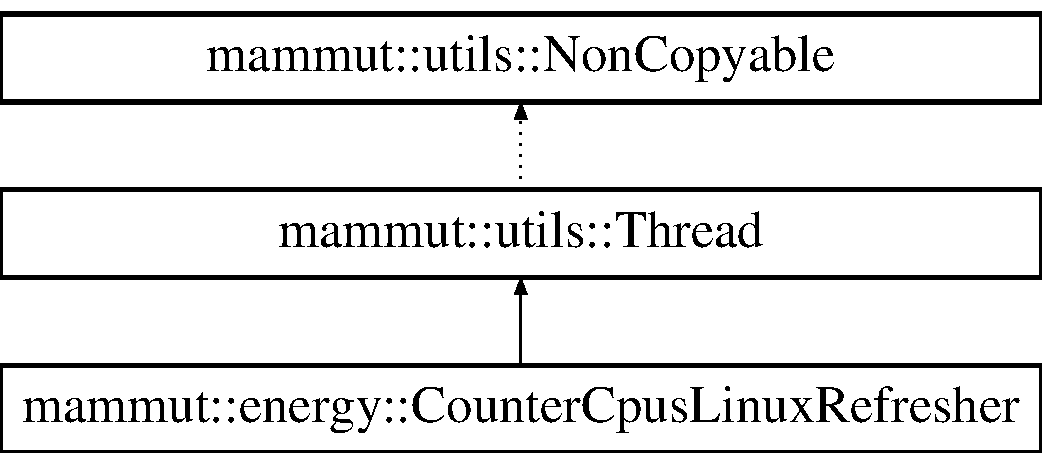
\includegraphics[height=3.000000cm]{classmammut_1_1energy_1_1CounterCpusLinuxRefresher}
\end{center}
\end{figure}
\subsection*{Public Member Functions}
\begin{DoxyCompactItemize}
\item 
\hypertarget{classmammut_1_1energy_1_1CounterCpusLinuxRefresher_aad08a6b27e6091ee7698ac5fbe0fe3fc}{{\bfseries Counter\-Cpus\-Linux\-Refresher} (\hyperlink{classmammut_1_1energy_1_1CounterCpusLinux}{Counter\-Cpus\-Linux} $\ast$counter)}\label{classmammut_1_1energy_1_1CounterCpusLinuxRefresher_aad08a6b27e6091ee7698ac5fbe0fe3fc}

\item 
void \hyperlink{classmammut_1_1energy_1_1CounterCpusLinuxRefresher_a9037ed7260ba2eea4995ac35dc079eeb}{run} ()
\end{DoxyCompactItemize}


\subsection{Member Function Documentation}
\hypertarget{classmammut_1_1energy_1_1CounterCpusLinuxRefresher_a9037ed7260ba2eea4995ac35dc079eeb}{\index{mammut\-::energy\-::\-Counter\-Cpus\-Linux\-Refresher@{mammut\-::energy\-::\-Counter\-Cpus\-Linux\-Refresher}!run@{run}}
\index{run@{run}!mammut::energy::CounterCpusLinuxRefresher@{mammut\-::energy\-::\-Counter\-Cpus\-Linux\-Refresher}}
\subsubsection[{run}]{\setlength{\rightskip}{0pt plus 5cm}void mammut\-::energy\-::\-Counter\-Cpus\-Linux\-Refresher\-::run (
\begin{DoxyParamCaption}
{}
\end{DoxyParamCaption}
)\hspace{0.3cm}{\ttfamily [virtual]}}}\label{classmammut_1_1energy_1_1CounterCpusLinuxRefresher_a9037ed7260ba2eea4995ac35dc079eeb}
This is the function that will be executed by the thread. To create a custom thread, is sufficient to extend this class and implement this pure member function. 

Implements \hyperlink{classmammut_1_1utils_1_1Thread_afc8a6df35c4f0417e6be899df973cca7}{mammut\-::utils\-::\-Thread}.



The documentation for this class was generated from the following files\-:\begin{DoxyCompactItemize}
\item 
/home/daniele/\-Code/\-Mammut/mammut/energy/energy-\/linux.\-hpp\item 
/home/daniele/\-Code/\-Mammut/mammut/energy/energy-\/linux.\-cpp\end{DoxyCompactItemize}

\hypertarget{classmammut_1_1energy_1_1CounterCpusRemote}{\section{mammut\-:\-:energy\-:\-:Counter\-Cpus\-Remote Class Reference}
\label{classmammut_1_1energy_1_1CounterCpusRemote}\index{mammut\-::energy\-::\-Counter\-Cpus\-Remote@{mammut\-::energy\-::\-Counter\-Cpus\-Remote}}
}
Inheritance diagram for mammut\-:\-:energy\-:\-:Counter\-Cpus\-Remote\-:\begin{figure}[H]
\begin{center}
\leavevmode
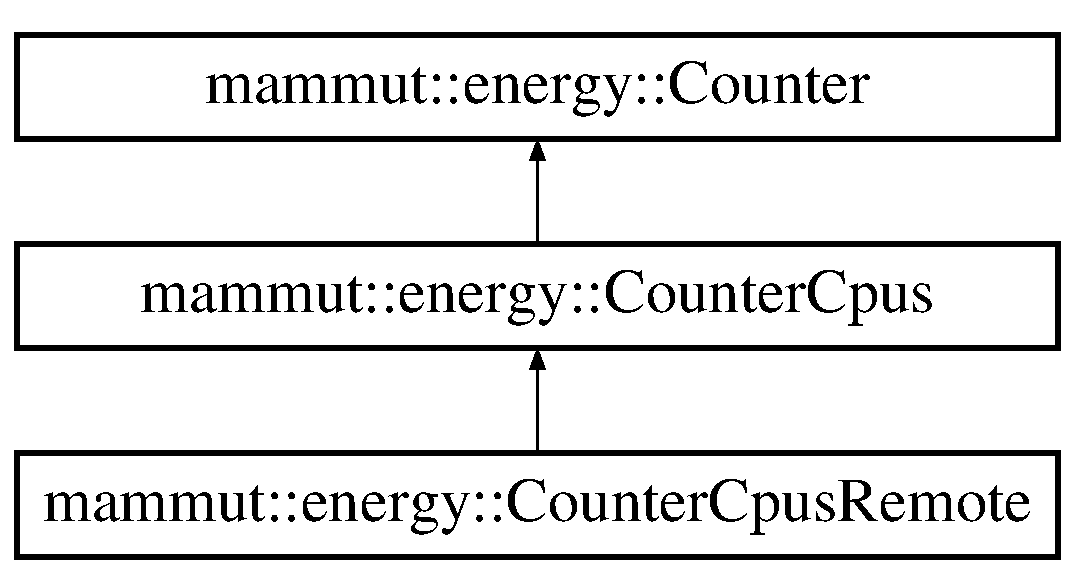
\includegraphics[height=3.000000cm]{classmammut_1_1energy_1_1CounterCpusRemote}
\end{center}
\end{figure}
\subsection*{Public Member Functions}
\begin{DoxyCompactItemize}
\item 
\hypertarget{classmammut_1_1energy_1_1CounterCpusRemote_aa56624f5cad1a23cc5fc50b2bdb60a02}{{\bfseries Counter\-Cpus\-Remote} (\hyperlink{classmammut_1_1Communicator}{mammut\-::\-Communicator} $\ast$const communicator)}\label{classmammut_1_1energy_1_1CounterCpusRemote_aa56624f5cad1a23cc5fc50b2bdb60a02}

\item 
\hypertarget{classmammut_1_1energy_1_1CounterCpusRemote_acee999bb9b7170e6128cff24ee135a39}{\hyperlink{classmammut_1_1energy_1_1JoulesCpu}{Joules\-Cpu} {\bfseries get\-Joules\-Components} ()}\label{classmammut_1_1energy_1_1CounterCpusRemote_acee999bb9b7170e6128cff24ee135a39}

\item 
\hyperlink{classmammut_1_1energy_1_1JoulesCpu}{Joules\-Cpu} \hyperlink{classmammut_1_1energy_1_1CounterCpusRemote_a01ade74cb22a24f39d294257d764fbf3}{get\-Joules\-Components} (topology\-::\-Cpu\-Id cpu\-Id)
\item 
\hypertarget{classmammut_1_1energy_1_1CounterCpusRemote_a9cabce3a60a6b55a7d7a7b807474d68d}{Joules {\bfseries get\-Joules\-Cpu} ()}\label{classmammut_1_1energy_1_1CounterCpusRemote_a9cabce3a60a6b55a7d7a7b807474d68d}

\item 
Joules \hyperlink{classmammut_1_1energy_1_1CounterCpusRemote_a1c55fc9f3bbcaed7d16e526175eca00c}{get\-Joules\-Cpu} (topology\-::\-Cpu\-Id cpu\-Id)
\item 
\hypertarget{classmammut_1_1energy_1_1CounterCpusRemote_a555fbad77c51f8cc45829d7a66570b37}{Joules {\bfseries get\-Joules\-Cores} ()}\label{classmammut_1_1energy_1_1CounterCpusRemote_a555fbad77c51f8cc45829d7a66570b37}

\item 
Joules \hyperlink{classmammut_1_1energy_1_1CounterCpusRemote_aa6f49a650b0df6aecb1e56ffeca15bd7}{get\-Joules\-Cores} (topology\-::\-Cpu\-Id cpu\-Id)
\item 
\hypertarget{classmammut_1_1energy_1_1CounterCpusRemote_aadd114f00607baadb4a9d449da8969ee}{Joules {\bfseries get\-Joules\-Graphic} ()}\label{classmammut_1_1energy_1_1CounterCpusRemote_aadd114f00607baadb4a9d449da8969ee}

\item 
Joules \hyperlink{classmammut_1_1energy_1_1CounterCpusRemote_af886a7df65acafc4bb762fb45a91bfaa}{get\-Joules\-Graphic} (topology\-::\-Cpu\-Id cpu\-Id)
\item 
\hypertarget{classmammut_1_1energy_1_1CounterCpusRemote_a668674116f076a30f1e908afcd3931c3}{Joules {\bfseries get\-Joules\-Dram} ()}\label{classmammut_1_1energy_1_1CounterCpusRemote_a668674116f076a30f1e908afcd3931c3}

\item 
Joules \hyperlink{classmammut_1_1energy_1_1CounterCpusRemote_a95558006c8d7e8453af38ff57ce0d3ff}{get\-Joules\-Dram} (topology\-::\-Cpu\-Id cpu\-Id)
\item 
bool \hyperlink{classmammut_1_1energy_1_1CounterCpusRemote_a7e50db0df2b842a7596e5ec559f477bf}{has\-Joules\-Dram} ()
\item 
bool \hyperlink{classmammut_1_1energy_1_1CounterCpusRemote_a315765ac4950dee79408301db828a834}{has\-Joules\-Graphic} ()
\item 
bool \hyperlink{classmammut_1_1energy_1_1CounterCpusRemote_a68203a642d22edc316c7b95bddfa4e15}{init} ()
\item 
void \hyperlink{classmammut_1_1energy_1_1CounterCpusRemote_a20439f71fc4d024be5470cec09bd0355}{reset} ()
\end{DoxyCompactItemize}
\subsection*{Additional Inherited Members}


\subsection{Member Function Documentation}
\hypertarget{classmammut_1_1energy_1_1CounterCpusRemote_a01ade74cb22a24f39d294257d764fbf3}{\index{mammut\-::energy\-::\-Counter\-Cpus\-Remote@{mammut\-::energy\-::\-Counter\-Cpus\-Remote}!get\-Joules\-Components@{get\-Joules\-Components}}
\index{get\-Joules\-Components@{get\-Joules\-Components}!mammut::energy::CounterCpusRemote@{mammut\-::energy\-::\-Counter\-Cpus\-Remote}}
\subsubsection[{get\-Joules\-Components}]{\setlength{\rightskip}{0pt plus 5cm}{\bf Joules\-Cpu} mammut\-::energy\-::\-Counter\-Cpus\-Remote\-::get\-Joules\-Components (
\begin{DoxyParamCaption}
\item[{topology\-::\-Cpu\-Id}]{cpu\-Id}
\end{DoxyParamCaption}
)\hspace{0.3cm}{\ttfamily [virtual]}}}\label{classmammut_1_1energy_1_1CounterCpusRemote_a01ade74cb22a24f39d294257d764fbf3}
Returns the Joules consumed by a Cpu and its components since the counter creation (or since the last call of \hyperlink{classmammut_1_1energy_1_1CounterCpusRemote_a20439f71fc4d024be5470cec09bd0355}{reset()}). 
\begin{DoxyParams}{Parameters}
{\em cpu\-Id} & The identifier of a Cpu. \\
\hline
\end{DoxyParams}
\begin{DoxyReturn}{Returns}
The Joules consumed by a Cpu and its components since the counter creation (or since the last call of \hyperlink{classmammut_1_1energy_1_1CounterCpusRemote_a20439f71fc4d024be5470cec09bd0355}{reset()}). 
\end{DoxyReturn}


Implements \hyperlink{classmammut_1_1energy_1_1CounterCpus_a4324fc4985dc89228450436db46551b7}{mammut\-::energy\-::\-Counter\-Cpus}.

\hypertarget{classmammut_1_1energy_1_1CounterCpusRemote_aa6f49a650b0df6aecb1e56ffeca15bd7}{\index{mammut\-::energy\-::\-Counter\-Cpus\-Remote@{mammut\-::energy\-::\-Counter\-Cpus\-Remote}!get\-Joules\-Cores@{get\-Joules\-Cores}}
\index{get\-Joules\-Cores@{get\-Joules\-Cores}!mammut::energy::CounterCpusRemote@{mammut\-::energy\-::\-Counter\-Cpus\-Remote}}
\subsubsection[{get\-Joules\-Cores}]{\setlength{\rightskip}{0pt plus 5cm}Joules mammut\-::energy\-::\-Counter\-Cpus\-Remote\-::get\-Joules\-Cores (
\begin{DoxyParamCaption}
\item[{topology\-::\-Cpu\-Id}]{cpu\-Id}
\end{DoxyParamCaption}
)\hspace{0.3cm}{\ttfamily [virtual]}}}\label{classmammut_1_1energy_1_1CounterCpusRemote_aa6f49a650b0df6aecb1e56ffeca15bd7}
Returns the Joules consumed by the cores of a Cpu since the counter creation (or since the last call of \hyperlink{classmammut_1_1energy_1_1CounterCpusRemote_a20439f71fc4d024be5470cec09bd0355}{reset()}). 
\begin{DoxyParams}{Parameters}
{\em cpu\-Id} & The identifier of a Cpu. \\
\hline
\end{DoxyParams}
\begin{DoxyReturn}{Returns}
The Joules consumed by the cores of a Cpu since the counter creation (or since the last call of \hyperlink{classmammut_1_1energy_1_1CounterCpusRemote_a20439f71fc4d024be5470cec09bd0355}{reset()}). 
\end{DoxyReturn}


Implements \hyperlink{classmammut_1_1energy_1_1CounterCpus_a2c041bbe181f593a50490a53a2729989}{mammut\-::energy\-::\-Counter\-Cpus}.

\hypertarget{classmammut_1_1energy_1_1CounterCpusRemote_a1c55fc9f3bbcaed7d16e526175eca00c}{\index{mammut\-::energy\-::\-Counter\-Cpus\-Remote@{mammut\-::energy\-::\-Counter\-Cpus\-Remote}!get\-Joules\-Cpu@{get\-Joules\-Cpu}}
\index{get\-Joules\-Cpu@{get\-Joules\-Cpu}!mammut::energy::CounterCpusRemote@{mammut\-::energy\-::\-Counter\-Cpus\-Remote}}
\subsubsection[{get\-Joules\-Cpu}]{\setlength{\rightskip}{0pt plus 5cm}Joules mammut\-::energy\-::\-Counter\-Cpus\-Remote\-::get\-Joules\-Cpu (
\begin{DoxyParamCaption}
\item[{topology\-::\-Cpu\-Id}]{cpu\-Id}
\end{DoxyParamCaption}
)\hspace{0.3cm}{\ttfamily [virtual]}}}\label{classmammut_1_1energy_1_1CounterCpusRemote_a1c55fc9f3bbcaed7d16e526175eca00c}
Returns the Joules consumed by a Cpu since the counter creation (or since the last call of \hyperlink{classmammut_1_1energy_1_1CounterCpusRemote_a20439f71fc4d024be5470cec09bd0355}{reset()}). 
\begin{DoxyParams}{Parameters}
{\em cpu\-Id} & The identifier of a Cpu. \\
\hline
\end{DoxyParams}
\begin{DoxyReturn}{Returns}
The Joules consumed by a Cpu since the counter creation (or since the last call of \hyperlink{classmammut_1_1energy_1_1CounterCpusRemote_a20439f71fc4d024be5470cec09bd0355}{reset()}). 
\end{DoxyReturn}


Implements \hyperlink{classmammut_1_1energy_1_1CounterCpus_a80c1f90abccce3f3ab621f08f7141f78}{mammut\-::energy\-::\-Counter\-Cpus}.

\hypertarget{classmammut_1_1energy_1_1CounterCpusRemote_a95558006c8d7e8453af38ff57ce0d3ff}{\index{mammut\-::energy\-::\-Counter\-Cpus\-Remote@{mammut\-::energy\-::\-Counter\-Cpus\-Remote}!get\-Joules\-Dram@{get\-Joules\-Dram}}
\index{get\-Joules\-Dram@{get\-Joules\-Dram}!mammut::energy::CounterCpusRemote@{mammut\-::energy\-::\-Counter\-Cpus\-Remote}}
\subsubsection[{get\-Joules\-Dram}]{\setlength{\rightskip}{0pt plus 5cm}Joules mammut\-::energy\-::\-Counter\-Cpus\-Remote\-::get\-Joules\-Dram (
\begin{DoxyParamCaption}
\item[{topology\-::\-Cpu\-Id}]{cpu\-Id}
\end{DoxyParamCaption}
)\hspace{0.3cm}{\ttfamily [virtual]}}}\label{classmammut_1_1energy_1_1CounterCpusRemote_a95558006c8d7e8453af38ff57ce0d3ff}
Returns the Joules consumed by a Cpu Dram since the counter creation (or since the last call of \hyperlink{classmammut_1_1energy_1_1CounterCpusRemote_a20439f71fc4d024be5470cec09bd0355}{reset()}). 
\begin{DoxyParams}{Parameters}
{\em cpu\-Id} & The identifier of a Cpu. \\
\hline
\end{DoxyParams}
\begin{DoxyReturn}{Returns}
The Joules consumed by a Cpu Dram since the counter creation (or since the last call of \hyperlink{classmammut_1_1energy_1_1CounterCpusRemote_a20439f71fc4d024be5470cec09bd0355}{reset()}). 
\end{DoxyReturn}


Implements \hyperlink{classmammut_1_1energy_1_1CounterCpus_a832e466d0a1f40f347d9a0211059a762}{mammut\-::energy\-::\-Counter\-Cpus}.

\hypertarget{classmammut_1_1energy_1_1CounterCpusRemote_af886a7df65acafc4bb762fb45a91bfaa}{\index{mammut\-::energy\-::\-Counter\-Cpus\-Remote@{mammut\-::energy\-::\-Counter\-Cpus\-Remote}!get\-Joules\-Graphic@{get\-Joules\-Graphic}}
\index{get\-Joules\-Graphic@{get\-Joules\-Graphic}!mammut::energy::CounterCpusRemote@{mammut\-::energy\-::\-Counter\-Cpus\-Remote}}
\subsubsection[{get\-Joules\-Graphic}]{\setlength{\rightskip}{0pt plus 5cm}Joules mammut\-::energy\-::\-Counter\-Cpus\-Remote\-::get\-Joules\-Graphic (
\begin{DoxyParamCaption}
\item[{topology\-::\-Cpu\-Id}]{cpu\-Id}
\end{DoxyParamCaption}
)\hspace{0.3cm}{\ttfamily [virtual]}}}\label{classmammut_1_1energy_1_1CounterCpusRemote_af886a7df65acafc4bb762fb45a91bfaa}
Returns the Joules consumed by a Cpu integrated graphic card (if present) since the counter creation (or since the last call of \hyperlink{classmammut_1_1energy_1_1CounterCpusRemote_a20439f71fc4d024be5470cec09bd0355}{reset()}). 
\begin{DoxyParams}{Parameters}
{\em cpu\-Id} & The identifier of a Cpu. \\
\hline
\end{DoxyParams}
\begin{DoxyReturn}{Returns}
The Joules consumed by a Cpu integrated graphic card (if present) since the counter creation (or since the last call of \hyperlink{classmammut_1_1energy_1_1CounterCpusRemote_a20439f71fc4d024be5470cec09bd0355}{reset()}). 
\end{DoxyReturn}


Implements \hyperlink{classmammut_1_1energy_1_1CounterCpus_a436f91199f40af85ce1b561781f24459}{mammut\-::energy\-::\-Counter\-Cpus}.

\hypertarget{classmammut_1_1energy_1_1CounterCpusRemote_a7e50db0df2b842a7596e5ec559f477bf}{\index{mammut\-::energy\-::\-Counter\-Cpus\-Remote@{mammut\-::energy\-::\-Counter\-Cpus\-Remote}!has\-Joules\-Dram@{has\-Joules\-Dram}}
\index{has\-Joules\-Dram@{has\-Joules\-Dram}!mammut::energy::CounterCpusRemote@{mammut\-::energy\-::\-Counter\-Cpus\-Remote}}
\subsubsection[{has\-Joules\-Dram}]{\setlength{\rightskip}{0pt plus 5cm}bool mammut\-::energy\-::\-Counter\-Cpus\-Remote\-::has\-Joules\-Dram (
\begin{DoxyParamCaption}
{}
\end{DoxyParamCaption}
)\hspace{0.3cm}{\ttfamily [virtual]}}}\label{classmammut_1_1energy_1_1CounterCpusRemote_a7e50db0df2b842a7596e5ec559f477bf}
Returns true if the counter for D\-R\-A\-M is present, false otherwise. \begin{DoxyReturn}{Returns}
True if the counter for D\-R\-A\-M is present, false otherwise. 
\end{DoxyReturn}


Implements \hyperlink{classmammut_1_1energy_1_1CounterCpus_a3d8c64aac5808275abdb2b01a31cbc11}{mammut\-::energy\-::\-Counter\-Cpus}.

\hypertarget{classmammut_1_1energy_1_1CounterCpusRemote_a315765ac4950dee79408301db828a834}{\index{mammut\-::energy\-::\-Counter\-Cpus\-Remote@{mammut\-::energy\-::\-Counter\-Cpus\-Remote}!has\-Joules\-Graphic@{has\-Joules\-Graphic}}
\index{has\-Joules\-Graphic@{has\-Joules\-Graphic}!mammut::energy::CounterCpusRemote@{mammut\-::energy\-::\-Counter\-Cpus\-Remote}}
\subsubsection[{has\-Joules\-Graphic}]{\setlength{\rightskip}{0pt plus 5cm}bool mammut\-::energy\-::\-Counter\-Cpus\-Remote\-::has\-Joules\-Graphic (
\begin{DoxyParamCaption}
{}
\end{DoxyParamCaption}
)\hspace{0.3cm}{\ttfamily [virtual]}}}\label{classmammut_1_1energy_1_1CounterCpusRemote_a315765ac4950dee79408301db828a834}
Returns true if the counter for integrated graphic card is present, false otherwise. \begin{DoxyReturn}{Returns}
True if the counter for integrated graphic card is present, false otherwise. 
\end{DoxyReturn}


Implements \hyperlink{classmammut_1_1energy_1_1CounterCpus_a94de30741049ba2131bcac532b8e7c8e}{mammut\-::energy\-::\-Counter\-Cpus}.

\hypertarget{classmammut_1_1energy_1_1CounterCpusRemote_a68203a642d22edc316c7b95bddfa4e15}{\index{mammut\-::energy\-::\-Counter\-Cpus\-Remote@{mammut\-::energy\-::\-Counter\-Cpus\-Remote}!init@{init}}
\index{init@{init}!mammut::energy::CounterCpusRemote@{mammut\-::energy\-::\-Counter\-Cpus\-Remote}}
\subsubsection[{init}]{\setlength{\rightskip}{0pt plus 5cm}bool mammut\-::energy\-::\-Counter\-Cpus\-Remote\-::init (
\begin{DoxyParamCaption}
{}
\end{DoxyParamCaption}
)\hspace{0.3cm}{\ttfamily [virtual]}}}\label{classmammut_1_1energy_1_1CounterCpusRemote_a68203a642d22edc316c7b95bddfa4e15}
Initializes the counter. \begin{DoxyReturn}{Returns}
True if the counter is present, false otherwise. 
\end{DoxyReturn}


Implements \hyperlink{classmammut_1_1energy_1_1CounterCpus_af4496166c7b79cd60fe57baa4b6e72a1}{mammut\-::energy\-::\-Counter\-Cpus}.

\hypertarget{classmammut_1_1energy_1_1CounterCpusRemote_a20439f71fc4d024be5470cec09bd0355}{\index{mammut\-::energy\-::\-Counter\-Cpus\-Remote@{mammut\-::energy\-::\-Counter\-Cpus\-Remote}!reset@{reset}}
\index{reset@{reset}!mammut::energy::CounterCpusRemote@{mammut\-::energy\-::\-Counter\-Cpus\-Remote}}
\subsubsection[{reset}]{\setlength{\rightskip}{0pt plus 5cm}void mammut\-::energy\-::\-Counter\-Cpus\-Remote\-::reset (
\begin{DoxyParamCaption}
{}
\end{DoxyParamCaption}
)\hspace{0.3cm}{\ttfamily [virtual]}}}\label{classmammut_1_1energy_1_1CounterCpusRemote_a20439f71fc4d024be5470cec09bd0355}
Resets the value of the counter. 

Implements \hyperlink{classmammut_1_1energy_1_1CounterCpus_ac3d2b3c06119c5e4f077b05689b2374a}{mammut\-::energy\-::\-Counter\-Cpus}.



The documentation for this class was generated from the following file\-:\begin{DoxyCompactItemize}
\item 
/home/daniele/\-Code/\-Mammut/mammut/energy/energy-\/remote.\-hpp\end{DoxyCompactItemize}

\hypertarget{classmammut_1_1energy_1_1CounterPlug}{\section{mammut\-:\-:energy\-:\-:Counter\-Plug Class Reference}
\label{classmammut_1_1energy_1_1CounterPlug}\index{mammut\-::energy\-::\-Counter\-Plug@{mammut\-::energy\-::\-Counter\-Plug}}
}
Inheritance diagram for mammut\-:\-:energy\-:\-:Counter\-Plug\-:\begin{figure}[H]
\begin{center}
\leavevmode
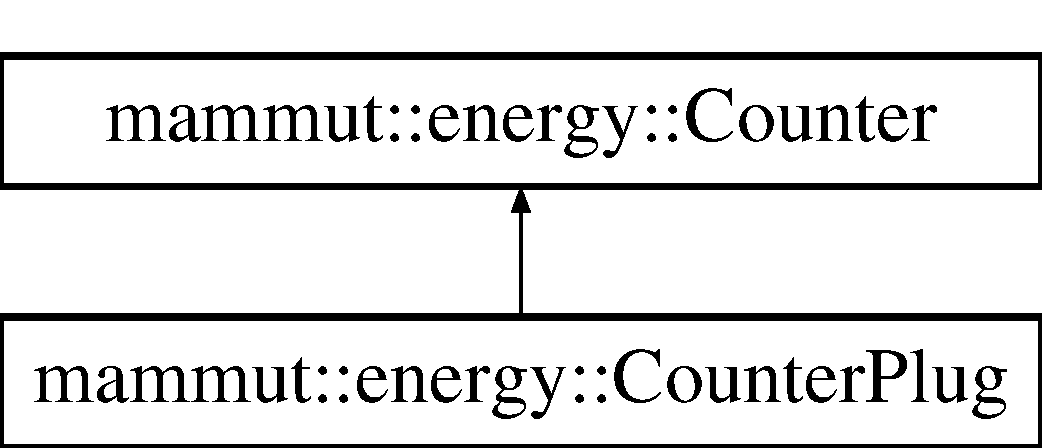
\includegraphics[height=2.000000cm]{classmammut_1_1energy_1_1CounterPlug}
\end{center}
\end{figure}
\subsection*{Public Member Functions}
\begin{DoxyCompactItemize}
\item 
virtual Joules \hyperlink{classmammut_1_1energy_1_1CounterPlug_a8ec0fc2cfe74fe23a0111493eac46be1}{get\-Joules} ()=0
\item 
virtual void \hyperlink{classmammut_1_1energy_1_1CounterPlug_af4ad1d14e69381f29ab53e1f5563eb1c}{reset} ()=0
\item 
virtual bool \hyperlink{classmammut_1_1energy_1_1CounterPlug_ac1bbf21f8936e19e5d5380e45cbc604b}{init} ()=0
\item 
Counter\-Type \hyperlink{classmammut_1_1energy_1_1CounterPlug_a1622556a5778ac5348b48cae705bd1d9}{get\-Type} ()
\end{DoxyCompactItemize}


\subsection{Member Function Documentation}
\hypertarget{classmammut_1_1energy_1_1CounterPlug_a8ec0fc2cfe74fe23a0111493eac46be1}{\index{mammut\-::energy\-::\-Counter\-Plug@{mammut\-::energy\-::\-Counter\-Plug}!get\-Joules@{get\-Joules}}
\index{get\-Joules@{get\-Joules}!mammut::energy::CounterPlug@{mammut\-::energy\-::\-Counter\-Plug}}
\subsubsection[{get\-Joules}]{\setlength{\rightskip}{0pt plus 5cm}virtual Joules mammut\-::energy\-::\-Counter\-Plug\-::get\-Joules (
\begin{DoxyParamCaption}
{}
\end{DoxyParamCaption}
)\hspace{0.3cm}{\ttfamily [pure virtual]}}}\label{classmammut_1_1energy_1_1CounterPlug_a8ec0fc2cfe74fe23a0111493eac46be1}
Returns the joules consumed up to this moment. \begin{DoxyReturn}{Returns}
The joules consumed up to this moment. 
\end{DoxyReturn}


Implements \hyperlink{classmammut_1_1energy_1_1Counter_a96b08f6fb969940cc5f5ee294b3b2a4a}{mammut\-::energy\-::\-Counter}.

\hypertarget{classmammut_1_1energy_1_1CounterPlug_a1622556a5778ac5348b48cae705bd1d9}{\index{mammut\-::energy\-::\-Counter\-Plug@{mammut\-::energy\-::\-Counter\-Plug}!get\-Type@{get\-Type}}
\index{get\-Type@{get\-Type}!mammut::energy::CounterPlug@{mammut\-::energy\-::\-Counter\-Plug}}
\subsubsection[{get\-Type}]{\setlength{\rightskip}{0pt plus 5cm}Counter\-Type mammut\-::energy\-::\-Counter\-Plug\-::get\-Type (
\begin{DoxyParamCaption}
{}
\end{DoxyParamCaption}
)\hspace{0.3cm}{\ttfamily [inline]}, {\ttfamily [virtual]}}}\label{classmammut_1_1energy_1_1CounterPlug_a1622556a5778ac5348b48cae705bd1d9}
Returns the type of this counter. \begin{DoxyReturn}{Returns}
The type of this counter. 
\end{DoxyReturn}


Implements \hyperlink{classmammut_1_1energy_1_1Counter_a6787edd9de68d900b937656a0899a954}{mammut\-::energy\-::\-Counter}.

\hypertarget{classmammut_1_1energy_1_1CounterPlug_ac1bbf21f8936e19e5d5380e45cbc604b}{\index{mammut\-::energy\-::\-Counter\-Plug@{mammut\-::energy\-::\-Counter\-Plug}!init@{init}}
\index{init@{init}!mammut::energy::CounterPlug@{mammut\-::energy\-::\-Counter\-Plug}}
\subsubsection[{init}]{\setlength{\rightskip}{0pt plus 5cm}virtual bool mammut\-::energy\-::\-Counter\-Plug\-::init (
\begin{DoxyParamCaption}
{}
\end{DoxyParamCaption}
)\hspace{0.3cm}{\ttfamily [pure virtual]}}}\label{classmammut_1_1energy_1_1CounterPlug_ac1bbf21f8936e19e5d5380e45cbc604b}
Initializes the counter. \begin{DoxyReturn}{Returns}
True if the counter is present, false otherwise. 
\end{DoxyReturn}


Implements \hyperlink{classmammut_1_1energy_1_1Counter_abd57eea0488bd5ff8377af9ea6add7f2}{mammut\-::energy\-::\-Counter}.

\hypertarget{classmammut_1_1energy_1_1CounterPlug_af4ad1d14e69381f29ab53e1f5563eb1c}{\index{mammut\-::energy\-::\-Counter\-Plug@{mammut\-::energy\-::\-Counter\-Plug}!reset@{reset}}
\index{reset@{reset}!mammut::energy::CounterPlug@{mammut\-::energy\-::\-Counter\-Plug}}
\subsubsection[{reset}]{\setlength{\rightskip}{0pt plus 5cm}virtual void mammut\-::energy\-::\-Counter\-Plug\-::reset (
\begin{DoxyParamCaption}
{}
\end{DoxyParamCaption}
)\hspace{0.3cm}{\ttfamily [pure virtual]}}}\label{classmammut_1_1energy_1_1CounterPlug_af4ad1d14e69381f29ab53e1f5563eb1c}
Resets the value of the counter. 

Implements \hyperlink{classmammut_1_1energy_1_1Counter_aa31fb6f9fa1139a2fe3c41019801cefe}{mammut\-::energy\-::\-Counter}.



The documentation for this class was generated from the following file\-:\begin{DoxyCompactItemize}
\item 
/home/daniele/\-Code/\-Mammut/mammut/energy/energy.\-hpp\end{DoxyCompactItemize}

\hypertarget{classmammut_1_1energy_1_1CounterPlugLinux}{\section{mammut\-:\-:energy\-:\-:Counter\-Plug\-Linux Class Reference}
\label{classmammut_1_1energy_1_1CounterPlugLinux}\index{mammut\-::energy\-::\-Counter\-Plug\-Linux@{mammut\-::energy\-::\-Counter\-Plug\-Linux}}
}
Inheritance diagram for mammut\-:\-:energy\-:\-:Counter\-Plug\-Linux\-:\begin{figure}[H]
\begin{center}
\leavevmode
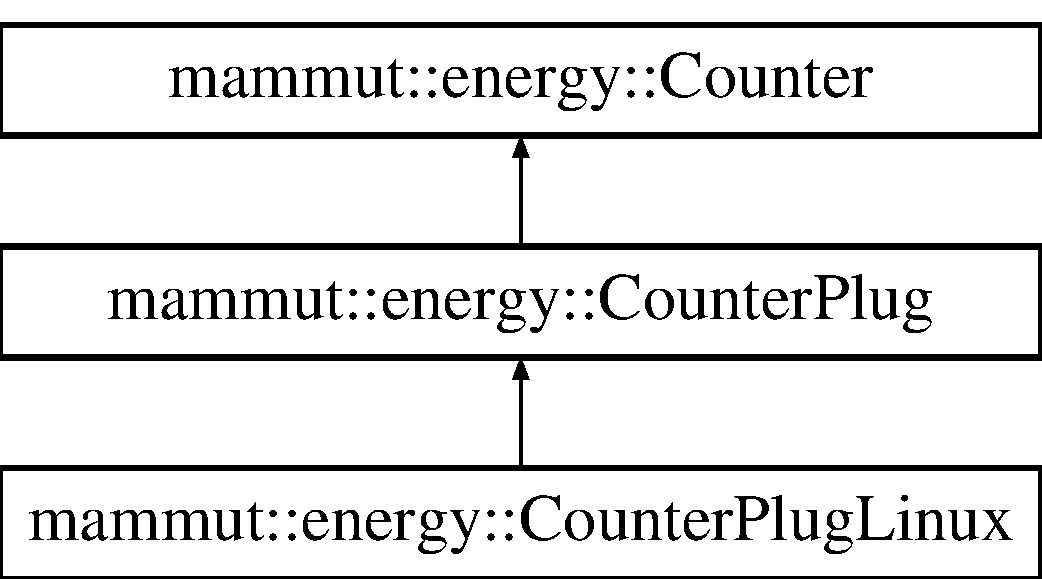
\includegraphics[height=3.000000cm]{classmammut_1_1energy_1_1CounterPlugLinux}
\end{center}
\end{figure}
\subsection*{Public Member Functions}
\begin{DoxyCompactItemize}
\item 
bool \hyperlink{classmammut_1_1energy_1_1CounterPlugLinux_a52064efe053f0096af344d1c9f2ac772}{init} ()
\item 
Joules \hyperlink{classmammut_1_1energy_1_1CounterPlugLinux_a94d9dd485b5a4f138c0e5e69a96640e9}{get\-Joules} ()
\item 
void \hyperlink{classmammut_1_1energy_1_1CounterPlugLinux_adafd0049576115f67c90fd2a128e2325}{reset} ()
\end{DoxyCompactItemize}


\subsection{Member Function Documentation}
\hypertarget{classmammut_1_1energy_1_1CounterPlugLinux_a94d9dd485b5a4f138c0e5e69a96640e9}{\index{mammut\-::energy\-::\-Counter\-Plug\-Linux@{mammut\-::energy\-::\-Counter\-Plug\-Linux}!get\-Joules@{get\-Joules}}
\index{get\-Joules@{get\-Joules}!mammut::energy::CounterPlugLinux@{mammut\-::energy\-::\-Counter\-Plug\-Linux}}
\subsubsection[{get\-Joules}]{\setlength{\rightskip}{0pt plus 5cm}Joules mammut\-::energy\-::\-Counter\-Plug\-Linux\-::get\-Joules (
\begin{DoxyParamCaption}
{}
\end{DoxyParamCaption}
)\hspace{0.3cm}{\ttfamily [virtual]}}}\label{classmammut_1_1energy_1_1CounterPlugLinux_a94d9dd485b5a4f138c0e5e69a96640e9}
Returns the joules consumed up to this moment. \begin{DoxyReturn}{Returns}
The joules consumed up to this moment. 
\end{DoxyReturn}


Implements \hyperlink{classmammut_1_1energy_1_1CounterPlug_a8ec0fc2cfe74fe23a0111493eac46be1}{mammut\-::energy\-::\-Counter\-Plug}.

\hypertarget{classmammut_1_1energy_1_1CounterPlugLinux_a52064efe053f0096af344d1c9f2ac772}{\index{mammut\-::energy\-::\-Counter\-Plug\-Linux@{mammut\-::energy\-::\-Counter\-Plug\-Linux}!init@{init}}
\index{init@{init}!mammut::energy::CounterPlugLinux@{mammut\-::energy\-::\-Counter\-Plug\-Linux}}
\subsubsection[{init}]{\setlength{\rightskip}{0pt plus 5cm}bool mammut\-::energy\-::\-Counter\-Plug\-Linux\-::init (
\begin{DoxyParamCaption}
{}
\end{DoxyParamCaption}
)\hspace{0.3cm}{\ttfamily [virtual]}}}\label{classmammut_1_1energy_1_1CounterPlugLinux_a52064efe053f0096af344d1c9f2ac772}
Initializes the counter. \begin{DoxyReturn}{Returns}
True if the counter is present, false otherwise. 
\end{DoxyReturn}


Implements \hyperlink{classmammut_1_1energy_1_1CounterPlug_ac1bbf21f8936e19e5d5380e45cbc604b}{mammut\-::energy\-::\-Counter\-Plug}.

\hypertarget{classmammut_1_1energy_1_1CounterPlugLinux_adafd0049576115f67c90fd2a128e2325}{\index{mammut\-::energy\-::\-Counter\-Plug\-Linux@{mammut\-::energy\-::\-Counter\-Plug\-Linux}!reset@{reset}}
\index{reset@{reset}!mammut::energy::CounterPlugLinux@{mammut\-::energy\-::\-Counter\-Plug\-Linux}}
\subsubsection[{reset}]{\setlength{\rightskip}{0pt plus 5cm}void mammut\-::energy\-::\-Counter\-Plug\-Linux\-::reset (
\begin{DoxyParamCaption}
{}
\end{DoxyParamCaption}
)\hspace{0.3cm}{\ttfamily [virtual]}}}\label{classmammut_1_1energy_1_1CounterPlugLinux_adafd0049576115f67c90fd2a128e2325}
Resets the value of the counter. 

Implements \hyperlink{classmammut_1_1energy_1_1CounterPlug_af4ad1d14e69381f29ab53e1f5563eb1c}{mammut\-::energy\-::\-Counter\-Plug}.



The documentation for this class was generated from the following files\-:\begin{DoxyCompactItemize}
\item 
/home/daniele/\-Code/\-Mammut/mammut/energy/energy-\/linux.\-hpp\item 
/home/daniele/\-Code/\-Mammut/mammut/energy/energy-\/linux.\-cpp\end{DoxyCompactItemize}

\hypertarget{classmammut_1_1energy_1_1CounterPlugRemote}{\section{mammut\-:\-:energy\-:\-:Counter\-Plug\-Remote Class Reference}
\label{classmammut_1_1energy_1_1CounterPlugRemote}\index{mammut\-::energy\-::\-Counter\-Plug\-Remote@{mammut\-::energy\-::\-Counter\-Plug\-Remote}}
}
Inheritance diagram for mammut\-:\-:energy\-:\-:Counter\-Plug\-Remote\-:\begin{figure}[H]
\begin{center}
\leavevmode
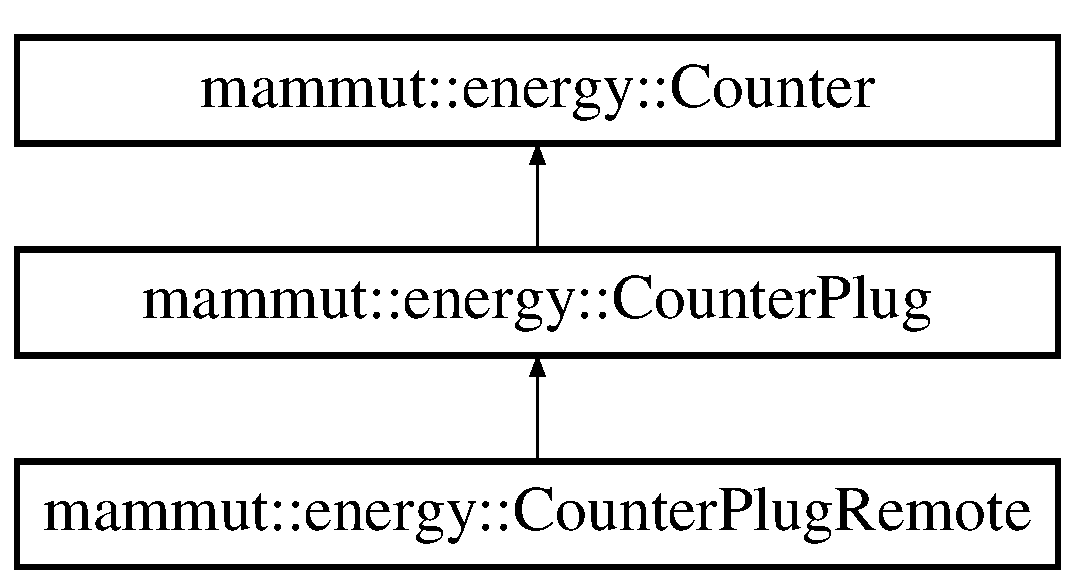
\includegraphics[height=3.000000cm]{classmammut_1_1energy_1_1CounterPlugRemote}
\end{center}
\end{figure}
\subsection*{Public Member Functions}
\begin{DoxyCompactItemize}
\item 
\hypertarget{classmammut_1_1energy_1_1CounterPlugRemote_a065a0b1dc8f570567ef674ddeae411b2}{{\bfseries Counter\-Plug\-Remote} (\hyperlink{classmammut_1_1Communicator}{mammut\-::\-Communicator} $\ast$const communicator)}\label{classmammut_1_1energy_1_1CounterPlugRemote_a065a0b1dc8f570567ef674ddeae411b2}

\item 
bool \hyperlink{classmammut_1_1energy_1_1CounterPlugRemote_a2b1b020d6e52ecfcbdd1dadbac76b811}{init} ()
\item 
Joules \hyperlink{classmammut_1_1energy_1_1CounterPlugRemote_abb17aa05e15e07ee8d2da213001147c0}{get\-Joules} ()
\item 
void \hyperlink{classmammut_1_1energy_1_1CounterPlugRemote_ad7436fd2c1d6b860e1bcbea5207f9357}{reset} ()
\end{DoxyCompactItemize}


\subsection{Member Function Documentation}
\hypertarget{classmammut_1_1energy_1_1CounterPlugRemote_abb17aa05e15e07ee8d2da213001147c0}{\index{mammut\-::energy\-::\-Counter\-Plug\-Remote@{mammut\-::energy\-::\-Counter\-Plug\-Remote}!get\-Joules@{get\-Joules}}
\index{get\-Joules@{get\-Joules}!mammut::energy::CounterPlugRemote@{mammut\-::energy\-::\-Counter\-Plug\-Remote}}
\subsubsection[{get\-Joules}]{\setlength{\rightskip}{0pt plus 5cm}Joules mammut\-::energy\-::\-Counter\-Plug\-Remote\-::get\-Joules (
\begin{DoxyParamCaption}
{}
\end{DoxyParamCaption}
)\hspace{0.3cm}{\ttfamily [virtual]}}}\label{classmammut_1_1energy_1_1CounterPlugRemote_abb17aa05e15e07ee8d2da213001147c0}
Returns the joules consumed up to this moment. \begin{DoxyReturn}{Returns}
The joules consumed up to this moment. 
\end{DoxyReturn}


Implements \hyperlink{classmammut_1_1energy_1_1CounterPlug_a8ec0fc2cfe74fe23a0111493eac46be1}{mammut\-::energy\-::\-Counter\-Plug}.

\hypertarget{classmammut_1_1energy_1_1CounterPlugRemote_a2b1b020d6e52ecfcbdd1dadbac76b811}{\index{mammut\-::energy\-::\-Counter\-Plug\-Remote@{mammut\-::energy\-::\-Counter\-Plug\-Remote}!init@{init}}
\index{init@{init}!mammut::energy::CounterPlugRemote@{mammut\-::energy\-::\-Counter\-Plug\-Remote}}
\subsubsection[{init}]{\setlength{\rightskip}{0pt plus 5cm}bool mammut\-::energy\-::\-Counter\-Plug\-Remote\-::init (
\begin{DoxyParamCaption}
{}
\end{DoxyParamCaption}
)\hspace{0.3cm}{\ttfamily [virtual]}}}\label{classmammut_1_1energy_1_1CounterPlugRemote_a2b1b020d6e52ecfcbdd1dadbac76b811}
Initializes the counter. \begin{DoxyReturn}{Returns}
True if the counter is present, false otherwise. 
\end{DoxyReturn}


Implements \hyperlink{classmammut_1_1energy_1_1CounterPlug_ac1bbf21f8936e19e5d5380e45cbc604b}{mammut\-::energy\-::\-Counter\-Plug}.

\hypertarget{classmammut_1_1energy_1_1CounterPlugRemote_ad7436fd2c1d6b860e1bcbea5207f9357}{\index{mammut\-::energy\-::\-Counter\-Plug\-Remote@{mammut\-::energy\-::\-Counter\-Plug\-Remote}!reset@{reset}}
\index{reset@{reset}!mammut::energy::CounterPlugRemote@{mammut\-::energy\-::\-Counter\-Plug\-Remote}}
\subsubsection[{reset}]{\setlength{\rightskip}{0pt plus 5cm}void mammut\-::energy\-::\-Counter\-Plug\-Remote\-::reset (
\begin{DoxyParamCaption}
{}
\end{DoxyParamCaption}
)\hspace{0.3cm}{\ttfamily [virtual]}}}\label{classmammut_1_1energy_1_1CounterPlugRemote_ad7436fd2c1d6b860e1bcbea5207f9357}
Resets the value of the counter. 

Implements \hyperlink{classmammut_1_1energy_1_1CounterPlug_af4ad1d14e69381f29ab53e1f5563eb1c}{mammut\-::energy\-::\-Counter\-Plug}.



The documentation for this class was generated from the following file\-:\begin{DoxyCompactItemize}
\item 
/home/daniele/\-Code/\-Mammut/mammut/energy/energy-\/remote.\-hpp\end{DoxyCompactItemize}

\hypertarget{classmammut_1_1topology_1_1Cpu}{\section{mammut\-:\-:topology\-:\-:Cpu Class Reference}
\label{classmammut_1_1topology_1_1Cpu}\index{mammut\-::topology\-::\-Cpu@{mammut\-::topology\-::\-Cpu}}
}
Inheritance diagram for mammut\-:\-:topology\-:\-:Cpu\-:\begin{figure}[H]
\begin{center}
\leavevmode
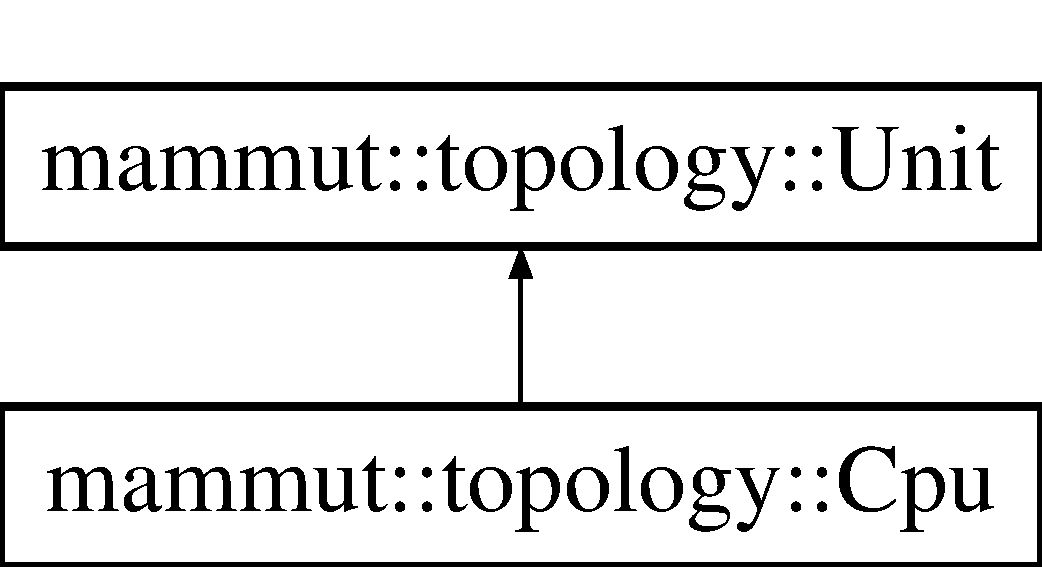
\includegraphics[height=3.000000cm]{classmammut_1_1topology_1_1Cpu}
\end{center}
\end{figure}
\subsection*{Public Member Functions}
\begin{DoxyCompactItemize}
\item 
Cpu\-Id \hyperlink{classmammut_1_1topology_1_1Cpu_ab8f01a27491ad5bc899e99374279ae12}{get\-Cpu\-Id} () const 
\item 
std\-::vector$<$ \hyperlink{classmammut_1_1topology_1_1PhysicalCore}{Physical\-Core} $\ast$ $>$ \hyperlink{classmammut_1_1topology_1_1Cpu_a1edbe9813dab7ea1c2eed9276c4ef9e9}{get\-Physical\-Cores} () const 
\item 
std\-::vector$<$ \hyperlink{classmammut_1_1topology_1_1VirtualCore}{Virtual\-Core} $\ast$ $>$ \hyperlink{classmammut_1_1topology_1_1Cpu_a06cb0216f32933242733a4768f7a9e32}{get\-Virtual\-Cores} () const 
\item 
\hyperlink{classmammut_1_1topology_1_1PhysicalCore}{Physical\-Core} $\ast$ \hyperlink{classmammut_1_1topology_1_1Cpu_aa773de6864b1b00609abc4f3167529cf}{get\-Physical\-Core} (Physical\-Core\-Id physical\-Core\-Id) const 
\item 
\hyperlink{classmammut_1_1topology_1_1VirtualCore}{Virtual\-Core} $\ast$ \hyperlink{classmammut_1_1topology_1_1Cpu_a577fbb46e774bd0d84100cf4d9909350}{get\-Virtual\-Core} (Virtual\-Core\-Id virtual\-Core\-Id) const 
\item 
\hyperlink{classmammut_1_1topology_1_1VirtualCore}{Virtual\-Core} $\ast$ \hyperlink{classmammut_1_1topology_1_1Cpu_ab814276f1e71a5036f1673751d132c8b}{get\-Virtual\-Core} () const 
\item 
virtual std\-::string \hyperlink{classmammut_1_1topology_1_1Cpu_a7b1fcfcc8df09588832ca1dc6351e6f1}{get\-Vendor\-Id} () const =0
\item 
virtual std\-::string \hyperlink{classmammut_1_1topology_1_1Cpu_a14f0984b504c0c207250829728193f8c}{get\-Family} () const =0
\item 
virtual std\-::string \hyperlink{classmammut_1_1topology_1_1Cpu_a6e98555afbc9d4985acc4ec30fbc5d96}{get\-Model} () const =0
\item 
virtual void \hyperlink{classmammut_1_1topology_1_1Cpu_a249829ade28b8fffcda1d2666cf68997}{maximize\-Utilization} () const =0
\item 
virtual void \hyperlink{classmammut_1_1topology_1_1Cpu_a3eea41d7ad6200d83301102f23944de5}{reset\-Utilization} () const =0
\end{DoxyCompactItemize}
\subsection*{Protected Member Functions}
\begin{DoxyCompactItemize}
\item 
\hypertarget{classmammut_1_1topology_1_1Cpu_a4a0b062cc466fb3e2fba89eeb959b72b}{{\bfseries Cpu} (Cpu\-Id cpu\-Id, std\-::vector$<$ \hyperlink{classmammut_1_1topology_1_1PhysicalCore}{Physical\-Core} $\ast$ $>$ physical\-Cores)}\label{classmammut_1_1topology_1_1Cpu_a4a0b062cc466fb3e2fba89eeb959b72b}

\end{DoxyCompactItemize}
\subsection*{Protected Attributes}
\begin{DoxyCompactItemize}
\item 
\hypertarget{classmammut_1_1topology_1_1Cpu_a9d1c9b790b7b2ecc254f1936d35c6210}{const Cpu\-Id {\bfseries \-\_\-cpu\-Id}}\label{classmammut_1_1topology_1_1Cpu_a9d1c9b790b7b2ecc254f1936d35c6210}

\item 
\hypertarget{classmammut_1_1topology_1_1Cpu_a9eee9dd8b3d7e223ada75c0d0be08fd9}{const std\-::vector$<$ \hyperlink{classmammut_1_1topology_1_1PhysicalCore}{Physical\-Core} $\ast$ $>$ {\bfseries \-\_\-physical\-Cores}}\label{classmammut_1_1topology_1_1Cpu_a9eee9dd8b3d7e223ada75c0d0be08fd9}

\item 
\hypertarget{classmammut_1_1topology_1_1Cpu_aa6ad4ed0b1314eb6282ca9bd84dc5e8b}{const std\-::vector$<$ \hyperlink{classmammut_1_1topology_1_1VirtualCore}{Virtual\-Core} $\ast$ $>$ {\bfseries \-\_\-virtual\-Cores}}\label{classmammut_1_1topology_1_1Cpu_aa6ad4ed0b1314eb6282ca9bd84dc5e8b}

\end{DoxyCompactItemize}


\subsection{Member Function Documentation}
\hypertarget{classmammut_1_1topology_1_1Cpu_ab8f01a27491ad5bc899e99374279ae12}{\index{mammut\-::topology\-::\-Cpu@{mammut\-::topology\-::\-Cpu}!get\-Cpu\-Id@{get\-Cpu\-Id}}
\index{get\-Cpu\-Id@{get\-Cpu\-Id}!mammut::topology::Cpu@{mammut\-::topology\-::\-Cpu}}
\subsubsection[{get\-Cpu\-Id}]{\setlength{\rightskip}{0pt plus 5cm}Cpu\-Id mammut\-::topology\-::\-Cpu\-::get\-Cpu\-Id (
\begin{DoxyParamCaption}
{}
\end{DoxyParamCaption}
) const}}\label{classmammut_1_1topology_1_1Cpu_ab8f01a27491ad5bc899e99374279ae12}
Returns the identifier of this C\-P\-U. \begin{DoxyReturn}{Returns}
The identifier of this C\-P\-U. 
\end{DoxyReturn}
\hypertarget{classmammut_1_1topology_1_1Cpu_a14f0984b504c0c207250829728193f8c}{\index{mammut\-::topology\-::\-Cpu@{mammut\-::topology\-::\-Cpu}!get\-Family@{get\-Family}}
\index{get\-Family@{get\-Family}!mammut::topology::Cpu@{mammut\-::topology\-::\-Cpu}}
\subsubsection[{get\-Family}]{\setlength{\rightskip}{0pt plus 5cm}virtual std\-::string mammut\-::topology\-::\-Cpu\-::get\-Family (
\begin{DoxyParamCaption}
{}
\end{DoxyParamCaption}
) const\hspace{0.3cm}{\ttfamily [pure virtual]}}}\label{classmammut_1_1topology_1_1Cpu_a14f0984b504c0c207250829728193f8c}
Returns the family of this \hyperlink{classmammut_1_1topology_1_1Cpu}{Cpu}. \begin{DoxyReturn}{Returns}
The family of this \hyperlink{classmammut_1_1topology_1_1Cpu}{Cpu}. 
\end{DoxyReturn}


Implemented in \hyperlink{classmammut_1_1topology_1_1CpuLinux_af6d293f96505b4269d0e763588ec538f}{mammut\-::topology\-::\-Cpu\-Linux}, and \hyperlink{classmammut_1_1topology_1_1CpuRemote_aacd6e5bee5d9b348220749efc614b6d1}{mammut\-::topology\-::\-Cpu\-Remote}.

\hypertarget{classmammut_1_1topology_1_1Cpu_a6e98555afbc9d4985acc4ec30fbc5d96}{\index{mammut\-::topology\-::\-Cpu@{mammut\-::topology\-::\-Cpu}!get\-Model@{get\-Model}}
\index{get\-Model@{get\-Model}!mammut::topology::Cpu@{mammut\-::topology\-::\-Cpu}}
\subsubsection[{get\-Model}]{\setlength{\rightskip}{0pt plus 5cm}virtual std\-::string mammut\-::topology\-::\-Cpu\-::get\-Model (
\begin{DoxyParamCaption}
{}
\end{DoxyParamCaption}
) const\hspace{0.3cm}{\ttfamily [pure virtual]}}}\label{classmammut_1_1topology_1_1Cpu_a6e98555afbc9d4985acc4ec30fbc5d96}
Returns the model of this \hyperlink{classmammut_1_1topology_1_1Cpu}{Cpu}. \begin{DoxyReturn}{Returns}
The model of this \hyperlink{classmammut_1_1topology_1_1Cpu}{Cpu}. 
\end{DoxyReturn}


Implemented in \hyperlink{classmammut_1_1topology_1_1CpuLinux_ad1fe33a16052441fd0ed67734452b984}{mammut\-::topology\-::\-Cpu\-Linux}, and \hyperlink{classmammut_1_1topology_1_1CpuRemote_a7d57ba15fa3db7f444c5757c5da93bdb}{mammut\-::topology\-::\-Cpu\-Remote}.

\hypertarget{classmammut_1_1topology_1_1Cpu_aa773de6864b1b00609abc4f3167529cf}{\index{mammut\-::topology\-::\-Cpu@{mammut\-::topology\-::\-Cpu}!get\-Physical\-Core@{get\-Physical\-Core}}
\index{get\-Physical\-Core@{get\-Physical\-Core}!mammut::topology::Cpu@{mammut\-::topology\-::\-Cpu}}
\subsubsection[{get\-Physical\-Core}]{\setlength{\rightskip}{0pt plus 5cm}{\bf Physical\-Core} $\ast$ mammut\-::topology\-::\-Cpu\-::get\-Physical\-Core (
\begin{DoxyParamCaption}
\item[{Physical\-Core\-Id}]{physical\-Core\-Id}
\end{DoxyParamCaption}
) const}}\label{classmammut_1_1topology_1_1Cpu_aa773de6864b1b00609abc4f3167529cf}
Returns the physical core with the given identifier, or N\-U\-L\-L if it is not present on this C\-P\-U. 
\begin{DoxyParams}{Parameters}
{\em physical\-Core\-Id} & The identifier of the physical core. \\
\hline
\end{DoxyParams}
\begin{DoxyReturn}{Returns}
The physical core with the given identifier, or N\-U\-L\-L if it is not present on this C\-P\-U. 
\end{DoxyReturn}
\hypertarget{classmammut_1_1topology_1_1Cpu_a1edbe9813dab7ea1c2eed9276c4ef9e9}{\index{mammut\-::topology\-::\-Cpu@{mammut\-::topology\-::\-Cpu}!get\-Physical\-Cores@{get\-Physical\-Cores}}
\index{get\-Physical\-Cores@{get\-Physical\-Cores}!mammut::topology::Cpu@{mammut\-::topology\-::\-Cpu}}
\subsubsection[{get\-Physical\-Cores}]{\setlength{\rightskip}{0pt plus 5cm}std\-::vector$<$ {\bf Physical\-Core} $\ast$ $>$ mammut\-::topology\-::\-Cpu\-::get\-Physical\-Cores (
\begin{DoxyParamCaption}
{}
\end{DoxyParamCaption}
) const}}\label{classmammut_1_1topology_1_1Cpu_a1edbe9813dab7ea1c2eed9276c4ef9e9}
Returns the physical cores of this C\-P\-U. \begin{DoxyReturn}{Returns}
A vector of physical cores. 
\end{DoxyReturn}
\hypertarget{classmammut_1_1topology_1_1Cpu_a7b1fcfcc8df09588832ca1dc6351e6f1}{\index{mammut\-::topology\-::\-Cpu@{mammut\-::topology\-::\-Cpu}!get\-Vendor\-Id@{get\-Vendor\-Id}}
\index{get\-Vendor\-Id@{get\-Vendor\-Id}!mammut::topology::Cpu@{mammut\-::topology\-::\-Cpu}}
\subsubsection[{get\-Vendor\-Id}]{\setlength{\rightskip}{0pt plus 5cm}virtual std\-::string mammut\-::topology\-::\-Cpu\-::get\-Vendor\-Id (
\begin{DoxyParamCaption}
{}
\end{DoxyParamCaption}
) const\hspace{0.3cm}{\ttfamily [pure virtual]}}}\label{classmammut_1_1topology_1_1Cpu_a7b1fcfcc8df09588832ca1dc6351e6f1}
Returns the vendor id of this \hyperlink{classmammut_1_1topology_1_1Cpu}{Cpu}. \begin{DoxyReturn}{Returns}
The vendor id of this \hyperlink{classmammut_1_1topology_1_1Cpu}{Cpu}. 
\end{DoxyReturn}


Implemented in \hyperlink{classmammut_1_1topology_1_1CpuLinux_a95f8d7d4f1d8fc23a4e3c0a7b7879be1}{mammut\-::topology\-::\-Cpu\-Linux}, and \hyperlink{classmammut_1_1topology_1_1CpuRemote_a3a49baf79550998a4d8782587cb27704}{mammut\-::topology\-::\-Cpu\-Remote}.

\hypertarget{classmammut_1_1topology_1_1Cpu_a577fbb46e774bd0d84100cf4d9909350}{\index{mammut\-::topology\-::\-Cpu@{mammut\-::topology\-::\-Cpu}!get\-Virtual\-Core@{get\-Virtual\-Core}}
\index{get\-Virtual\-Core@{get\-Virtual\-Core}!mammut::topology::Cpu@{mammut\-::topology\-::\-Cpu}}
\subsubsection[{get\-Virtual\-Core}]{\setlength{\rightskip}{0pt plus 5cm}{\bf Virtual\-Core} $\ast$ mammut\-::topology\-::\-Cpu\-::get\-Virtual\-Core (
\begin{DoxyParamCaption}
\item[{Virtual\-Core\-Id}]{virtual\-Core\-Id}
\end{DoxyParamCaption}
) const}}\label{classmammut_1_1topology_1_1Cpu_a577fbb46e774bd0d84100cf4d9909350}
Returns the virtual core with the given identifier, or N\-U\-L\-L if it is not present on this C\-P\-U. 
\begin{DoxyParams}{Parameters}
{\em virtual\-Core\-Id} & The identifier of the virtual core. \\
\hline
\end{DoxyParams}
\begin{DoxyReturn}{Returns}
The virtual core with the given identifier, or N\-U\-L\-L if it is not present on this C\-P\-U. 
\end{DoxyReturn}
\hypertarget{classmammut_1_1topology_1_1Cpu_ab814276f1e71a5036f1673751d132c8b}{\index{mammut\-::topology\-::\-Cpu@{mammut\-::topology\-::\-Cpu}!get\-Virtual\-Core@{get\-Virtual\-Core}}
\index{get\-Virtual\-Core@{get\-Virtual\-Core}!mammut::topology::Cpu@{mammut\-::topology\-::\-Cpu}}
\subsubsection[{get\-Virtual\-Core}]{\setlength{\rightskip}{0pt plus 5cm}{\bf Virtual\-Core} $\ast$ mammut\-::topology\-::\-Cpu\-::get\-Virtual\-Core (
\begin{DoxyParamCaption}
{}
\end{DoxyParamCaption}
) const}}\label{classmammut_1_1topology_1_1Cpu_ab814276f1e71a5036f1673751d132c8b}
Returns a virtual core belonging to this \hyperlink{classmammut_1_1topology_1_1Cpu}{Cpu}, or N\-U\-L\-L if it is not present. \begin{DoxyReturn}{Returns}
A virtual core belonging to this \hyperlink{classmammut_1_1topology_1_1Cpu}{Cpu}, or N\-U\-L\-L if it is not present. 
\end{DoxyReturn}
\hypertarget{classmammut_1_1topology_1_1Cpu_a06cb0216f32933242733a4768f7a9e32}{\index{mammut\-::topology\-::\-Cpu@{mammut\-::topology\-::\-Cpu}!get\-Virtual\-Cores@{get\-Virtual\-Cores}}
\index{get\-Virtual\-Cores@{get\-Virtual\-Cores}!mammut::topology::Cpu@{mammut\-::topology\-::\-Cpu}}
\subsubsection[{get\-Virtual\-Cores}]{\setlength{\rightskip}{0pt plus 5cm}std\-::vector$<$ {\bf Virtual\-Core} $\ast$ $>$ mammut\-::topology\-::\-Cpu\-::get\-Virtual\-Cores (
\begin{DoxyParamCaption}
{}
\end{DoxyParamCaption}
) const}}\label{classmammut_1_1topology_1_1Cpu_a06cb0216f32933242733a4768f7a9e32}
Returns the virtual cores of this C\-P\-U. \begin{DoxyReturn}{Returns}
A vector of virtual cores. 
\end{DoxyReturn}
\hypertarget{classmammut_1_1topology_1_1Cpu_a249829ade28b8fffcda1d2666cf68997}{\index{mammut\-::topology\-::\-Cpu@{mammut\-::topology\-::\-Cpu}!maximize\-Utilization@{maximize\-Utilization}}
\index{maximize\-Utilization@{maximize\-Utilization}!mammut::topology::Cpu@{mammut\-::topology\-::\-Cpu}}
\subsubsection[{maximize\-Utilization}]{\setlength{\rightskip}{0pt plus 5cm}virtual void mammut\-::topology\-::\-Cpu\-::maximize\-Utilization (
\begin{DoxyParamCaption}
{}
\end{DoxyParamCaption}
) const\hspace{0.3cm}{\ttfamily [pure virtual]}}}\label{classmammut_1_1topology_1_1Cpu_a249829ade28b8fffcda1d2666cf68997}
Bring the utilization of this C\-P\-U to 100\% until \hyperlink{classmammut_1_1topology_1_1Cpu_a3eea41d7ad6200d83301102f23944de5}{reset\-Utilization()} is called. 

Implements \hyperlink{classmammut_1_1topology_1_1Unit_a0a12d2b5939c609c657a2bd652801e88}{mammut\-::topology\-::\-Unit}.



Implemented in \hyperlink{classmammut_1_1topology_1_1CpuLinux_a428a9356fce899f82494f0973201f009}{mammut\-::topology\-::\-Cpu\-Linux}, and \hyperlink{classmammut_1_1topology_1_1CpuRemote_a1f25bdc6f2b049a831a03ba702699626}{mammut\-::topology\-::\-Cpu\-Remote}.

\hypertarget{classmammut_1_1topology_1_1Cpu_a3eea41d7ad6200d83301102f23944de5}{\index{mammut\-::topology\-::\-Cpu@{mammut\-::topology\-::\-Cpu}!reset\-Utilization@{reset\-Utilization}}
\index{reset\-Utilization@{reset\-Utilization}!mammut::topology::Cpu@{mammut\-::topology\-::\-Cpu}}
\subsubsection[{reset\-Utilization}]{\setlength{\rightskip}{0pt plus 5cm}virtual void mammut\-::topology\-::\-Cpu\-::reset\-Utilization (
\begin{DoxyParamCaption}
{}
\end{DoxyParamCaption}
) const\hspace{0.3cm}{\ttfamily [pure virtual]}}}\label{classmammut_1_1topology_1_1Cpu_a3eea41d7ad6200d83301102f23944de5}
Resets the utilization of this C\-P\-U. 

Implements \hyperlink{classmammut_1_1topology_1_1Unit_a70730dde75533d3f5ecd3d3686df87cc}{mammut\-::topology\-::\-Unit}.



Implemented in \hyperlink{classmammut_1_1topology_1_1CpuLinux_ae22825c9a86f221c3ffe9c456dfe96aa}{mammut\-::topology\-::\-Cpu\-Linux}, and \hyperlink{classmammut_1_1topology_1_1CpuRemote_a689af84ac46ab57081fc4fa47c9992b6}{mammut\-::topology\-::\-Cpu\-Remote}.



The documentation for this class was generated from the following files\-:\begin{DoxyCompactItemize}
\item 
/home/daniele/\-Code/\-Mammut/mammut/topology/topology.\-hpp\item 
/home/daniele/\-Code/\-Mammut/mammut/topology/topology.\-cpp\end{DoxyCompactItemize}

\hypertarget{classmammut_1_1cpufreq_1_1CpuFreq}{\section{mammut\-:\-:cpufreq\-:\-:Cpu\-Freq Class Reference}
\label{classmammut_1_1cpufreq_1_1CpuFreq}\index{mammut\-::cpufreq\-::\-Cpu\-Freq@{mammut\-::cpufreq\-::\-Cpu\-Freq}}
}
Inheritance diagram for mammut\-:\-:cpufreq\-:\-:Cpu\-Freq\-:\begin{figure}[H]
\begin{center}
\leavevmode
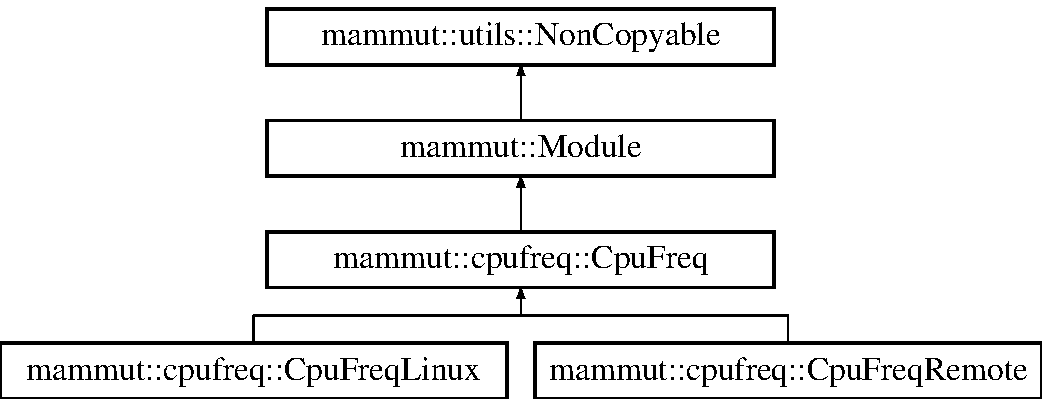
\includegraphics[height=4.000000cm]{classmammut_1_1cpufreq_1_1CpuFreq}
\end{center}
\end{figure}
\subsection*{Public Member Functions}
\begin{DoxyCompactItemize}
\item 
virtual std\-::vector$<$ \hyperlink{classmammut_1_1cpufreq_1_1Domain}{Domain} $\ast$ $>$ \hyperlink{classmammut_1_1cpufreq_1_1CpuFreq_a2ff7cb9b384f506f17340089bba3ba99}{get\-Domains} () const =0
\item 
\hyperlink{classmammut_1_1cpufreq_1_1Domain}{Domain} $\ast$ \hyperlink{classmammut_1_1cpufreq_1_1CpuFreq_aebb8f1ebd1977e817eda907c7107e672}{get\-Domain} (const \hyperlink{classmammut_1_1topology_1_1VirtualCore}{topology\-::\-Virtual\-Core} $\ast$virtual\-Core) const 
\item 
std\-::vector$<$ \hyperlink{classmammut_1_1cpufreq_1_1Domain}{Domain} $\ast$ $>$ \hyperlink{classmammut_1_1cpufreq_1_1CpuFreq_a7cdfd85b4e2d53a0aaee8261be8e3b28}{get\-Domains} (const std\-::vector$<$ \hyperlink{classmammut_1_1topology_1_1VirtualCore}{topology\-::\-Virtual\-Core} $\ast$ $>$ \&virtual\-Cores) const 
\item 
std\-::vector$<$ \hyperlink{classmammut_1_1cpufreq_1_1Domain}{Domain} $\ast$ $>$ \hyperlink{classmammut_1_1cpufreq_1_1CpuFreq_a81175ffbdaa8e4611aa2f550ad358798}{get\-Domains\-Complete} (const std\-::vector$<$ \hyperlink{classmammut_1_1topology_1_1VirtualCore}{topology\-::\-Virtual\-Core} $\ast$ $>$ \&virtual\-Cores) const 
\item 
std\-::vector$<$ \hyperlink{structmammut_1_1cpufreq_1_1RollbackPoint}{Rollback\-Point} $>$ \hyperlink{classmammut_1_1cpufreq_1_1CpuFreq_adf302de171b8c3011ef228f201a71802}{get\-Rollback\-Points} () const 
\item 
void \hyperlink{classmammut_1_1cpufreq_1_1CpuFreq_ac60f3fe79742135c124746e9e357f277}{rollback} (const std\-::vector$<$ \hyperlink{structmammut_1_1cpufreq_1_1RollbackPoint}{Rollback\-Point} $>$ \&rollback\-Points) const 
\item 
bool \hyperlink{classmammut_1_1cpufreq_1_1CpuFreq_a1fb40924ebe83f5840d8586f71696fef}{is\-Governor\-Available} (Governor governor) const 
\item 
virtual bool \hyperlink{classmammut_1_1cpufreq_1_1CpuFreq_a93c7855b33a6794ddb8ba1aa0d4a5496}{is\-Boosting\-Supported} () const =0
\item 
virtual bool \hyperlink{classmammut_1_1cpufreq_1_1CpuFreq_acc8da4a88e11b5e974a4877e2ff1ef95}{is\-Boosting\-Enabled} () const =0
\item 
virtual void \hyperlink{classmammut_1_1cpufreq_1_1CpuFreq_a53f6662c7cf58861d562266c95a61e8c}{enable\-Boosting} () const =0
\item 
virtual void \hyperlink{classmammut_1_1cpufreq_1_1CpuFreq_a8abff63046f3b4ce5b992d4716fdabd1}{disable\-Boosting} () const =0
\end{DoxyCompactItemize}
\subsection*{Static Public Member Functions}
\begin{DoxyCompactItemize}
\item 
static std\-::string \hyperlink{classmammut_1_1cpufreq_1_1CpuFreq_ad8ce7208e7edea078f12840ba56bf841}{get\-Governor\-Name\-From\-Governor} (Governor governor)
\item 
static Governor \hyperlink{classmammut_1_1cpufreq_1_1CpuFreq_ad5ae77529591173d35e073967d2603e0}{get\-Governor\-From\-Governor\-Name} (const std\-::string \&governor\-Name)
\end{DoxyCompactItemize}
\subsection*{Static Protected Member Functions}
\begin{DoxyCompactItemize}
\item 
static std\-::vector\\*
$<$ \hyperlink{classmammut_1_1topology_1_1VirtualCore}{topology\-::\-Virtual\-Core} $\ast$ $>$ \hyperlink{classmammut_1_1cpufreq_1_1CpuFreq_a7ca4c36e55240c5dea838da9ea09144d}{filter\-Virtual\-Cores} (const std\-::vector$<$ \hyperlink{classmammut_1_1topology_1_1VirtualCore}{topology\-::\-Virtual\-Core} $\ast$ $>$ \&virtual\-Cores, const std\-::vector$<$ topology\-::\-Virtual\-Core\-Id $>$ \&identifiers)
\end{DoxyCompactItemize}


\subsection{Member Function Documentation}
\hypertarget{classmammut_1_1cpufreq_1_1CpuFreq_a8abff63046f3b4ce5b992d4716fdabd1}{\index{mammut\-::cpufreq\-::\-Cpu\-Freq@{mammut\-::cpufreq\-::\-Cpu\-Freq}!disable\-Boosting@{disable\-Boosting}}
\index{disable\-Boosting@{disable\-Boosting}!mammut::cpufreq::CpuFreq@{mammut\-::cpufreq\-::\-Cpu\-Freq}}
\subsubsection[{disable\-Boosting}]{\setlength{\rightskip}{0pt plus 5cm}virtual void mammut\-::cpufreq\-::\-Cpu\-Freq\-::disable\-Boosting (
\begin{DoxyParamCaption}
{}
\end{DoxyParamCaption}
) const\hspace{0.3cm}{\ttfamily [pure virtual]}}}\label{classmammut_1_1cpufreq_1_1CpuFreq_a8abff63046f3b4ce5b992d4716fdabd1}
Disabled frequency boosting. 

Implemented in \hyperlink{classmammut_1_1cpufreq_1_1CpuFreqRemote_ac48475824e7dbd675418dc95ac1bdd1e}{mammut\-::cpufreq\-::\-Cpu\-Freq\-Remote}, and \hyperlink{classmammut_1_1cpufreq_1_1CpuFreqLinux_acb6ce2fcb128211bd899e0c057951db8}{mammut\-::cpufreq\-::\-Cpu\-Freq\-Linux}.

\hypertarget{classmammut_1_1cpufreq_1_1CpuFreq_a53f6662c7cf58861d562266c95a61e8c}{\index{mammut\-::cpufreq\-::\-Cpu\-Freq@{mammut\-::cpufreq\-::\-Cpu\-Freq}!enable\-Boosting@{enable\-Boosting}}
\index{enable\-Boosting@{enable\-Boosting}!mammut::cpufreq::CpuFreq@{mammut\-::cpufreq\-::\-Cpu\-Freq}}
\subsubsection[{enable\-Boosting}]{\setlength{\rightskip}{0pt plus 5cm}virtual void mammut\-::cpufreq\-::\-Cpu\-Freq\-::enable\-Boosting (
\begin{DoxyParamCaption}
{}
\end{DoxyParamCaption}
) const\hspace{0.3cm}{\ttfamily [pure virtual]}}}\label{classmammut_1_1cpufreq_1_1CpuFreq_a53f6662c7cf58861d562266c95a61e8c}
Enables frequency boosting. 

Implemented in \hyperlink{classmammut_1_1cpufreq_1_1CpuFreqRemote_a230fbe7271cf8091411a065477498140}{mammut\-::cpufreq\-::\-Cpu\-Freq\-Remote}, and \hyperlink{classmammut_1_1cpufreq_1_1CpuFreqLinux_a0c40ded518bf086d602f70035b29491b}{mammut\-::cpufreq\-::\-Cpu\-Freq\-Linux}.

\hypertarget{classmammut_1_1cpufreq_1_1CpuFreq_a7ca4c36e55240c5dea838da9ea09144d}{\index{mammut\-::cpufreq\-::\-Cpu\-Freq@{mammut\-::cpufreq\-::\-Cpu\-Freq}!filter\-Virtual\-Cores@{filter\-Virtual\-Cores}}
\index{filter\-Virtual\-Cores@{filter\-Virtual\-Cores}!mammut::cpufreq::CpuFreq@{mammut\-::cpufreq\-::\-Cpu\-Freq}}
\subsubsection[{filter\-Virtual\-Cores}]{\setlength{\rightskip}{0pt plus 5cm}std\-::vector$<$ {\bf topology\-::\-Virtual\-Core} $\ast$ $>$ mammut\-::cpufreq\-::\-Cpu\-Freq\-::filter\-Virtual\-Cores (
\begin{DoxyParamCaption}
\item[{const std\-::vector$<$ {\bf topology\-::\-Virtual\-Core} $\ast$ $>$ \&}]{virtual\-Cores, }
\item[{const std\-::vector$<$ topology\-::\-Virtual\-Core\-Id $>$ \&}]{identifiers}
\end{DoxyParamCaption}
)\hspace{0.3cm}{\ttfamily [static]}, {\ttfamily [protected]}}}\label{classmammut_1_1cpufreq_1_1CpuFreq_a7ca4c36e55240c5dea838da9ea09144d}
From a given set of virtual cores, returns only those with specified identifiers. 
\begin{DoxyParams}{Parameters}
{\em virtual\-Cores} & The set of virtual cores. \\
\hline
{\em identifiers} & The identifiers of the virtual cores we need. \\
\hline
\end{DoxyParams}
\begin{DoxyReturn}{Returns}
A set of virtual cores with the specified identifiers. 
\end{DoxyReturn}
\hypertarget{classmammut_1_1cpufreq_1_1CpuFreq_aebb8f1ebd1977e817eda907c7107e672}{\index{mammut\-::cpufreq\-::\-Cpu\-Freq@{mammut\-::cpufreq\-::\-Cpu\-Freq}!get\-Domain@{get\-Domain}}
\index{get\-Domain@{get\-Domain}!mammut::cpufreq::CpuFreq@{mammut\-::cpufreq\-::\-Cpu\-Freq}}
\subsubsection[{get\-Domain}]{\setlength{\rightskip}{0pt plus 5cm}{\bf Domain} $\ast$ mammut\-::cpufreq\-::\-Cpu\-Freq\-::get\-Domain (
\begin{DoxyParamCaption}
\item[{const {\bf topology\-::\-Virtual\-Core} $\ast$}]{virtual\-Core}
\end{DoxyParamCaption}
) const}}\label{classmammut_1_1cpufreq_1_1CpuFreq_aebb8f1ebd1977e817eda907c7107e672}
Gets the domain of a specified virtual core. 
\begin{DoxyParams}{Parameters}
{\em virtual\-Core} & The virtual core. \\
\hline
\end{DoxyParams}
\begin{DoxyReturn}{Returns}
The domain of the virtual core. 
\end{DoxyReturn}
\hypertarget{classmammut_1_1cpufreq_1_1CpuFreq_a2ff7cb9b384f506f17340089bba3ba99}{\index{mammut\-::cpufreq\-::\-Cpu\-Freq@{mammut\-::cpufreq\-::\-Cpu\-Freq}!get\-Domains@{get\-Domains}}
\index{get\-Domains@{get\-Domains}!mammut::cpufreq::CpuFreq@{mammut\-::cpufreq\-::\-Cpu\-Freq}}
\subsubsection[{get\-Domains}]{\setlength{\rightskip}{0pt plus 5cm}virtual std\-::vector$<${\bf Domain}$\ast$$>$ mammut\-::cpufreq\-::\-Cpu\-Freq\-::get\-Domains (
\begin{DoxyParamCaption}
{}
\end{DoxyParamCaption}
) const\hspace{0.3cm}{\ttfamily [pure virtual]}}}\label{classmammut_1_1cpufreq_1_1CpuFreq_a2ff7cb9b384f506f17340089bba3ba99}
Gets the domains division of the cores. \begin{DoxyReturn}{Returns}
A vector of domains. 
\end{DoxyReturn}


Implemented in \hyperlink{classmammut_1_1cpufreq_1_1CpuFreqRemote_a07b1ffad978a91b5179d339697ded144}{mammut\-::cpufreq\-::\-Cpu\-Freq\-Remote}, and \hyperlink{classmammut_1_1cpufreq_1_1CpuFreqLinux_a8c1129abc2edef364f1fabce4f434459}{mammut\-::cpufreq\-::\-Cpu\-Freq\-Linux}.

\hypertarget{classmammut_1_1cpufreq_1_1CpuFreq_a7cdfd85b4e2d53a0aaee8261be8e3b28}{\index{mammut\-::cpufreq\-::\-Cpu\-Freq@{mammut\-::cpufreq\-::\-Cpu\-Freq}!get\-Domains@{get\-Domains}}
\index{get\-Domains@{get\-Domains}!mammut::cpufreq::CpuFreq@{mammut\-::cpufreq\-::\-Cpu\-Freq}}
\subsubsection[{get\-Domains}]{\setlength{\rightskip}{0pt plus 5cm}std\-::vector$<$ {\bf Domain} $\ast$ $>$ mammut\-::cpufreq\-::\-Cpu\-Freq\-::get\-Domains (
\begin{DoxyParamCaption}
\item[{const std\-::vector$<$ {\bf topology\-::\-Virtual\-Core} $\ast$ $>$ \&}]{virtual\-Cores}
\end{DoxyParamCaption}
) const}}\label{classmammut_1_1cpufreq_1_1CpuFreq_a7cdfd85b4e2d53a0aaee8261be8e3b28}
Given a set of virtual cores, returns the domains to which these virtual cores belong. 
\begin{DoxyParams}{Parameters}
{\em virtual\-Cores} & The set of virtual cores. \\
\hline
\end{DoxyParams}
\begin{DoxyReturn}{Returns}
A vector of domains. 
\end{DoxyReturn}
\hypertarget{classmammut_1_1cpufreq_1_1CpuFreq_a81175ffbdaa8e4611aa2f550ad358798}{\index{mammut\-::cpufreq\-::\-Cpu\-Freq@{mammut\-::cpufreq\-::\-Cpu\-Freq}!get\-Domains\-Complete@{get\-Domains\-Complete}}
\index{get\-Domains\-Complete@{get\-Domains\-Complete}!mammut::cpufreq::CpuFreq@{mammut\-::cpufreq\-::\-Cpu\-Freq}}
\subsubsection[{get\-Domains\-Complete}]{\setlength{\rightskip}{0pt plus 5cm}std\-::vector$<$ {\bf Domain} $\ast$ $>$ mammut\-::cpufreq\-::\-Cpu\-Freq\-::get\-Domains\-Complete (
\begin{DoxyParamCaption}
\item[{const std\-::vector$<$ {\bf topology\-::\-Virtual\-Core} $\ast$ $>$ \&}]{virtual\-Cores}
\end{DoxyParamCaption}
) const}}\label{classmammut_1_1cpufreq_1_1CpuFreq_a81175ffbdaa8e4611aa2f550ad358798}
Given a set of virtual cores, returns the a vector of domains. The domains in this vector are only those who have all their virtual cores contained in the specified set. Accordingly, for each element D in the returned vector, D-\/$>$get\-Virtual\-Cores() will return a subset of virtual\-Cores parameter. 
\begin{DoxyParams}{Parameters}
{\em virtual\-Cores} & The set of virtual cores. \\
\hline
\end{DoxyParams}
\begin{DoxyReturn}{Returns}
A vector of domains. 
\end{DoxyReturn}
\hypertarget{classmammut_1_1cpufreq_1_1CpuFreq_ad5ae77529591173d35e073967d2603e0}{\index{mammut\-::cpufreq\-::\-Cpu\-Freq@{mammut\-::cpufreq\-::\-Cpu\-Freq}!get\-Governor\-From\-Governor\-Name@{get\-Governor\-From\-Governor\-Name}}
\index{get\-Governor\-From\-Governor\-Name@{get\-Governor\-From\-Governor\-Name}!mammut::cpufreq::CpuFreq@{mammut\-::cpufreq\-::\-Cpu\-Freq}}
\subsubsection[{get\-Governor\-From\-Governor\-Name}]{\setlength{\rightskip}{0pt plus 5cm}Governor mammut\-::cpufreq\-::\-Cpu\-Freq\-::get\-Governor\-From\-Governor\-Name (
\begin{DoxyParamCaption}
\item[{const std\-::string \&}]{governor\-Name}
\end{DoxyParamCaption}
)\hspace{0.3cm}{\ttfamily [static]}}}\label{classmammut_1_1cpufreq_1_1CpuFreq_ad5ae77529591173d35e073967d2603e0}
Returns the governor identifier starting from the name of the governor. 
\begin{DoxyParams}{Parameters}
{\em governor\-Name} & The name of the governor. \\
\hline
\end{DoxyParams}
\begin{DoxyReturn}{Returns}
The identifier associated to governor\-Name, or G\-O\-V\-E\-R\-N\-O\-R\-\_\-\-N\-U\-M if no association is present. 
\end{DoxyReturn}
\hypertarget{classmammut_1_1cpufreq_1_1CpuFreq_ad8ce7208e7edea078f12840ba56bf841}{\index{mammut\-::cpufreq\-::\-Cpu\-Freq@{mammut\-::cpufreq\-::\-Cpu\-Freq}!get\-Governor\-Name\-From\-Governor@{get\-Governor\-Name\-From\-Governor}}
\index{get\-Governor\-Name\-From\-Governor@{get\-Governor\-Name\-From\-Governor}!mammut::cpufreq::CpuFreq@{mammut\-::cpufreq\-::\-Cpu\-Freq}}
\subsubsection[{get\-Governor\-Name\-From\-Governor}]{\setlength{\rightskip}{0pt plus 5cm}std\-::string mammut\-::cpufreq\-::\-Cpu\-Freq\-::get\-Governor\-Name\-From\-Governor (
\begin{DoxyParamCaption}
\item[{Governor}]{governor}
\end{DoxyParamCaption}
)\hspace{0.3cm}{\ttfamily [static]}}}\label{classmammut_1_1cpufreq_1_1CpuFreq_ad8ce7208e7edea078f12840ba56bf841}
Returns the governor name associated to a specific identifier. 
\begin{DoxyParams}{Parameters}
{\em governor} & The identifier of the governor. \\
\hline
\end{DoxyParams}
\begin{DoxyReturn}{Returns}
The governor name associated to governor. 
\end{DoxyReturn}
\hypertarget{classmammut_1_1cpufreq_1_1CpuFreq_adf302de171b8c3011ef228f201a71802}{\index{mammut\-::cpufreq\-::\-Cpu\-Freq@{mammut\-::cpufreq\-::\-Cpu\-Freq}!get\-Rollback\-Points@{get\-Rollback\-Points}}
\index{get\-Rollback\-Points@{get\-Rollback\-Points}!mammut::cpufreq::CpuFreq@{mammut\-::cpufreq\-::\-Cpu\-Freq}}
\subsubsection[{get\-Rollback\-Points}]{\setlength{\rightskip}{0pt plus 5cm}std\-::vector$<$ {\bf Rollback\-Point} $>$ mammut\-::cpufreq\-::\-Cpu\-Freq\-::get\-Rollback\-Points (
\begin{DoxyParamCaption}
{}
\end{DoxyParamCaption}
) const}}\label{classmammut_1_1cpufreq_1_1CpuFreq_adf302de171b8c3011ef228f201a71802}
Returns a rollback point for each domain. They can be used to bring the domains back to the point when this function is called. \begin{DoxyReturn}{Returns}
A vector of rollback points. 
\end{DoxyReturn}
\hypertarget{classmammut_1_1cpufreq_1_1CpuFreq_acc8da4a88e11b5e974a4877e2ff1ef95}{\index{mammut\-::cpufreq\-::\-Cpu\-Freq@{mammut\-::cpufreq\-::\-Cpu\-Freq}!is\-Boosting\-Enabled@{is\-Boosting\-Enabled}}
\index{is\-Boosting\-Enabled@{is\-Boosting\-Enabled}!mammut::cpufreq::CpuFreq@{mammut\-::cpufreq\-::\-Cpu\-Freq}}
\subsubsection[{is\-Boosting\-Enabled}]{\setlength{\rightskip}{0pt plus 5cm}virtual bool mammut\-::cpufreq\-::\-Cpu\-Freq\-::is\-Boosting\-Enabled (
\begin{DoxyParamCaption}
{}
\end{DoxyParamCaption}
) const\hspace{0.3cm}{\ttfamily [pure virtual]}}}\label{classmammut_1_1cpufreq_1_1CpuFreq_acc8da4a88e11b5e974a4877e2ff1ef95}
Returns true if frequency boosting is enabled. \begin{DoxyReturn}{Returns}
True if frequency boosting is enabled, false otherwise. 
\end{DoxyReturn}


Implemented in \hyperlink{classmammut_1_1cpufreq_1_1CpuFreqRemote_aa08948a1c885cc0ebac412d6734f6cbb}{mammut\-::cpufreq\-::\-Cpu\-Freq\-Remote}, and \hyperlink{classmammut_1_1cpufreq_1_1CpuFreqLinux_a2c6cb213703975feac9b0170eb861f8d}{mammut\-::cpufreq\-::\-Cpu\-Freq\-Linux}.

\hypertarget{classmammut_1_1cpufreq_1_1CpuFreq_a93c7855b33a6794ddb8ba1aa0d4a5496}{\index{mammut\-::cpufreq\-::\-Cpu\-Freq@{mammut\-::cpufreq\-::\-Cpu\-Freq}!is\-Boosting\-Supported@{is\-Boosting\-Supported}}
\index{is\-Boosting\-Supported@{is\-Boosting\-Supported}!mammut::cpufreq::CpuFreq@{mammut\-::cpufreq\-::\-Cpu\-Freq}}
\subsubsection[{is\-Boosting\-Supported}]{\setlength{\rightskip}{0pt plus 5cm}virtual bool mammut\-::cpufreq\-::\-Cpu\-Freq\-::is\-Boosting\-Supported (
\begin{DoxyParamCaption}
{}
\end{DoxyParamCaption}
) const\hspace{0.3cm}{\ttfamily [pure virtual]}}}\label{classmammut_1_1cpufreq_1_1CpuFreq_a93c7855b33a6794ddb8ba1aa0d4a5496}
Returns true if frequency boosting is supported. \begin{DoxyReturn}{Returns}
True if frequency boosting is supported, false otherwise. 
\end{DoxyReturn}


Implemented in \hyperlink{classmammut_1_1cpufreq_1_1CpuFreqRemote_a5def353551f4f9e50c62ae3367532e40}{mammut\-::cpufreq\-::\-Cpu\-Freq\-Remote}, and \hyperlink{classmammut_1_1cpufreq_1_1CpuFreqLinux_afe44ce09634cb70a4106d4b1c4fe7a16}{mammut\-::cpufreq\-::\-Cpu\-Freq\-Linux}.

\hypertarget{classmammut_1_1cpufreq_1_1CpuFreq_a1fb40924ebe83f5840d8586f71696fef}{\index{mammut\-::cpufreq\-::\-Cpu\-Freq@{mammut\-::cpufreq\-::\-Cpu\-Freq}!is\-Governor\-Available@{is\-Governor\-Available}}
\index{is\-Governor\-Available@{is\-Governor\-Available}!mammut::cpufreq::CpuFreq@{mammut\-::cpufreq\-::\-Cpu\-Freq}}
\subsubsection[{is\-Governor\-Available}]{\setlength{\rightskip}{0pt plus 5cm}bool mammut\-::cpufreq\-::\-Cpu\-Freq\-::is\-Governor\-Available (
\begin{DoxyParamCaption}
\item[{Governor}]{governor}
\end{DoxyParamCaption}
) const}}\label{classmammut_1_1cpufreq_1_1CpuFreq_a1fb40924ebe83f5840d8586f71696fef}
Checks the availability of a specific governor. 
\begin{DoxyParams}{Parameters}
{\em governor} & The governor. \\
\hline
\end{DoxyParams}
\begin{DoxyReturn}{Returns}
True if the governor is available for all domains, false otherwise. 
\end{DoxyReturn}
\hypertarget{classmammut_1_1cpufreq_1_1CpuFreq_ac60f3fe79742135c124746e9e357f277}{\index{mammut\-::cpufreq\-::\-Cpu\-Freq@{mammut\-::cpufreq\-::\-Cpu\-Freq}!rollback@{rollback}}
\index{rollback@{rollback}!mammut::cpufreq::CpuFreq@{mammut\-::cpufreq\-::\-Cpu\-Freq}}
\subsubsection[{rollback}]{\setlength{\rightskip}{0pt plus 5cm}void mammut\-::cpufreq\-::\-Cpu\-Freq\-::rollback (
\begin{DoxyParamCaption}
\item[{const std\-::vector$<$ {\bf Rollback\-Point} $>$ \&}]{rollback\-Points}
\end{DoxyParamCaption}
) const}}\label{classmammut_1_1cpufreq_1_1CpuFreq_ac60f3fe79742135c124746e9e357f277}
Bring the domains to the respective rollback points. 
\begin{DoxyParams}{Parameters}
{\em rollback\-Points} & A vector of rollback points. \\
\hline
\end{DoxyParams}


The documentation for this class was generated from the following files\-:\begin{DoxyCompactItemize}
\item 
/home/daniele/\-Code/\-Mammut/mammut/cpufreq/cpufreq.\-hpp\item 
/home/daniele/\-Code/\-Mammut/mammut/cpufreq/cpufreq.\-cpp\end{DoxyCompactItemize}

\hypertarget{classmammut_1_1cpufreq_1_1CpuFreqLinux}{\section{mammut\-:\-:cpufreq\-:\-:Cpu\-Freq\-Linux Class Reference}
\label{classmammut_1_1cpufreq_1_1CpuFreqLinux}\index{mammut\-::cpufreq\-::\-Cpu\-Freq\-Linux@{mammut\-::cpufreq\-::\-Cpu\-Freq\-Linux}}
}
Inheritance diagram for mammut\-:\-:cpufreq\-:\-:Cpu\-Freq\-Linux\-:\begin{figure}[H]
\begin{center}
\leavevmode
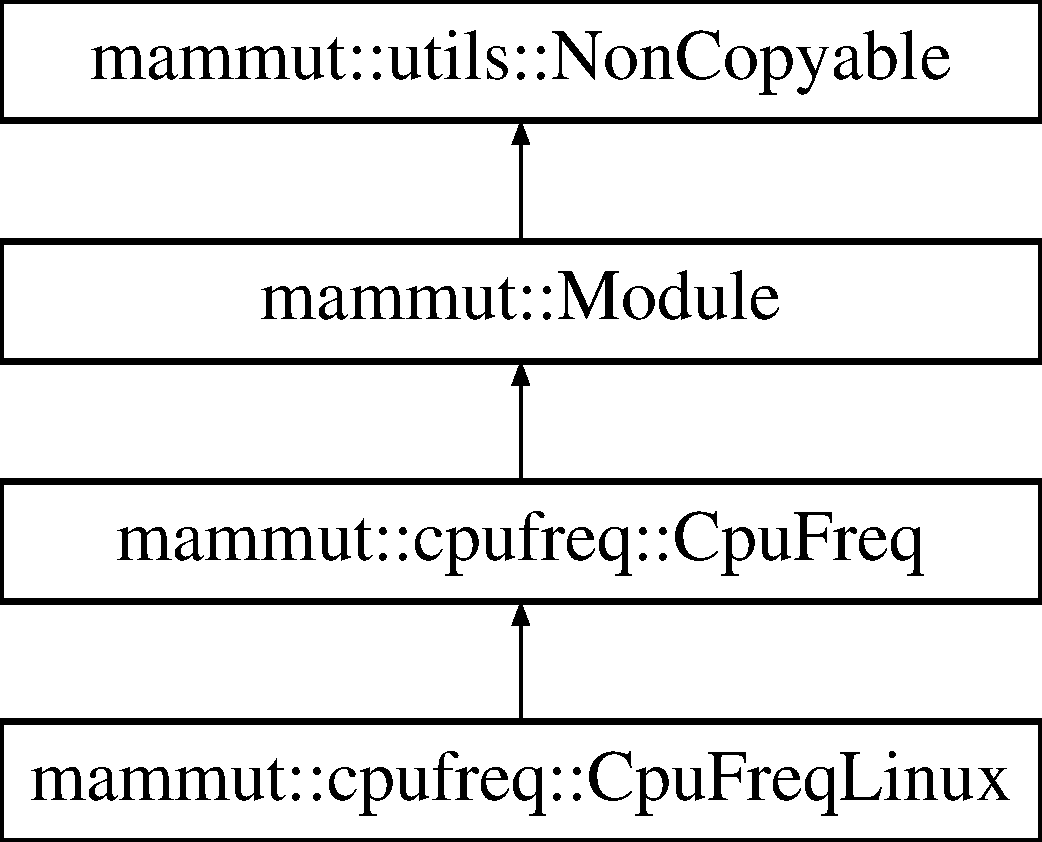
\includegraphics[height=4.000000cm]{classmammut_1_1cpufreq_1_1CpuFreqLinux}
\end{center}
\end{figure}
\subsection*{Public Member Functions}
\begin{DoxyCompactItemize}
\item 
\hyperlink{classmammut_1_1cpufreq_1_1CpuFreqLinux_ad80ab9dcd2a6c710c5b5734260dadb9c}{Cpu\-Freq\-Linux} ()
\item 
std\-::vector$<$ \hyperlink{classmammut_1_1cpufreq_1_1Domain}{Domain} $\ast$ $>$ \hyperlink{classmammut_1_1cpufreq_1_1CpuFreqLinux_a8c1129abc2edef364f1fabce4f434459}{get\-Domains} () const 
\item 
bool \hyperlink{classmammut_1_1cpufreq_1_1CpuFreqLinux_afe44ce09634cb70a4106d4b1c4fe7a16}{is\-Boosting\-Supported} () const 
\item 
bool \hyperlink{classmammut_1_1cpufreq_1_1CpuFreqLinux_a2c6cb213703975feac9b0170eb861f8d}{is\-Boosting\-Enabled} () const 
\item 
void \hyperlink{classmammut_1_1cpufreq_1_1CpuFreqLinux_a0c40ded518bf086d602f70035b29491b}{enable\-Boosting} () const 
\item 
void \hyperlink{classmammut_1_1cpufreq_1_1CpuFreqLinux_acb6ce2fcb128211bd899e0c057951db8}{disable\-Boosting} () const 
\end{DoxyCompactItemize}
\subsection*{Additional Inherited Members}


\subsection{Constructor \& Destructor Documentation}
\hypertarget{classmammut_1_1cpufreq_1_1CpuFreqLinux_ad80ab9dcd2a6c710c5b5734260dadb9c}{\index{mammut\-::cpufreq\-::\-Cpu\-Freq\-Linux@{mammut\-::cpufreq\-::\-Cpu\-Freq\-Linux}!Cpu\-Freq\-Linux@{Cpu\-Freq\-Linux}}
\index{Cpu\-Freq\-Linux@{Cpu\-Freq\-Linux}!mammut::cpufreq::CpuFreqLinux@{mammut\-::cpufreq\-::\-Cpu\-Freq\-Linux}}
\subsubsection[{Cpu\-Freq\-Linux}]{\setlength{\rightskip}{0pt plus 5cm}mammut\-::cpufreq\-::\-Cpu\-Freq\-Linux\-::\-Cpu\-Freq\-Linux (
\begin{DoxyParamCaption}
{}
\end{DoxyParamCaption}
)}}\label{classmammut_1_1cpufreq_1_1CpuFreqLinux_ad80ab9dcd2a6c710c5b5734260dadb9c}
If freqdomain\-\_\-cpus file are present, we must consider them instead of related\-\_\-cpus.

Converts the line to a vector of virtual cores identifiers.

Creates a domain based on the vector of cores identifiers. 

\subsection{Member Function Documentation}
\hypertarget{classmammut_1_1cpufreq_1_1CpuFreqLinux_acb6ce2fcb128211bd899e0c057951db8}{\index{mammut\-::cpufreq\-::\-Cpu\-Freq\-Linux@{mammut\-::cpufreq\-::\-Cpu\-Freq\-Linux}!disable\-Boosting@{disable\-Boosting}}
\index{disable\-Boosting@{disable\-Boosting}!mammut::cpufreq::CpuFreqLinux@{mammut\-::cpufreq\-::\-Cpu\-Freq\-Linux}}
\subsubsection[{disable\-Boosting}]{\setlength{\rightskip}{0pt plus 5cm}void mammut\-::cpufreq\-::\-Cpu\-Freq\-Linux\-::disable\-Boosting (
\begin{DoxyParamCaption}
{}
\end{DoxyParamCaption}
) const\hspace{0.3cm}{\ttfamily [virtual]}}}\label{classmammut_1_1cpufreq_1_1CpuFreqLinux_acb6ce2fcb128211bd899e0c057951db8}
Disabled frequency boosting. 

Implements \hyperlink{classmammut_1_1cpufreq_1_1CpuFreq_a8abff63046f3b4ce5b992d4716fdabd1}{mammut\-::cpufreq\-::\-Cpu\-Freq}.

\hypertarget{classmammut_1_1cpufreq_1_1CpuFreqLinux_a0c40ded518bf086d602f70035b29491b}{\index{mammut\-::cpufreq\-::\-Cpu\-Freq\-Linux@{mammut\-::cpufreq\-::\-Cpu\-Freq\-Linux}!enable\-Boosting@{enable\-Boosting}}
\index{enable\-Boosting@{enable\-Boosting}!mammut::cpufreq::CpuFreqLinux@{mammut\-::cpufreq\-::\-Cpu\-Freq\-Linux}}
\subsubsection[{enable\-Boosting}]{\setlength{\rightskip}{0pt plus 5cm}void mammut\-::cpufreq\-::\-Cpu\-Freq\-Linux\-::enable\-Boosting (
\begin{DoxyParamCaption}
{}
\end{DoxyParamCaption}
) const\hspace{0.3cm}{\ttfamily [virtual]}}}\label{classmammut_1_1cpufreq_1_1CpuFreqLinux_a0c40ded518bf086d602f70035b29491b}
Enables frequency boosting. 

Implements \hyperlink{classmammut_1_1cpufreq_1_1CpuFreq_a53f6662c7cf58861d562266c95a61e8c}{mammut\-::cpufreq\-::\-Cpu\-Freq}.

\hypertarget{classmammut_1_1cpufreq_1_1CpuFreqLinux_a8c1129abc2edef364f1fabce4f434459}{\index{mammut\-::cpufreq\-::\-Cpu\-Freq\-Linux@{mammut\-::cpufreq\-::\-Cpu\-Freq\-Linux}!get\-Domains@{get\-Domains}}
\index{get\-Domains@{get\-Domains}!mammut::cpufreq::CpuFreqLinux@{mammut\-::cpufreq\-::\-Cpu\-Freq\-Linux}}
\subsubsection[{get\-Domains}]{\setlength{\rightskip}{0pt plus 5cm}vector$<$ {\bf Domain} $\ast$ $>$ mammut\-::cpufreq\-::\-Cpu\-Freq\-Linux\-::get\-Domains (
\begin{DoxyParamCaption}
{}
\end{DoxyParamCaption}
) const\hspace{0.3cm}{\ttfamily [virtual]}}}\label{classmammut_1_1cpufreq_1_1CpuFreqLinux_a8c1129abc2edef364f1fabce4f434459}
Gets the domains division of the cores. \begin{DoxyReturn}{Returns}
A vector of domains. 
\end{DoxyReturn}


Implements \hyperlink{classmammut_1_1cpufreq_1_1CpuFreq_a2ff7cb9b384f506f17340089bba3ba99}{mammut\-::cpufreq\-::\-Cpu\-Freq}.

\hypertarget{classmammut_1_1cpufreq_1_1CpuFreqLinux_a2c6cb213703975feac9b0170eb861f8d}{\index{mammut\-::cpufreq\-::\-Cpu\-Freq\-Linux@{mammut\-::cpufreq\-::\-Cpu\-Freq\-Linux}!is\-Boosting\-Enabled@{is\-Boosting\-Enabled}}
\index{is\-Boosting\-Enabled@{is\-Boosting\-Enabled}!mammut::cpufreq::CpuFreqLinux@{mammut\-::cpufreq\-::\-Cpu\-Freq\-Linux}}
\subsubsection[{is\-Boosting\-Enabled}]{\setlength{\rightskip}{0pt plus 5cm}bool mammut\-::cpufreq\-::\-Cpu\-Freq\-Linux\-::is\-Boosting\-Enabled (
\begin{DoxyParamCaption}
{}
\end{DoxyParamCaption}
) const\hspace{0.3cm}{\ttfamily [virtual]}}}\label{classmammut_1_1cpufreq_1_1CpuFreqLinux_a2c6cb213703975feac9b0170eb861f8d}
Returns true if frequency boosting is enabled. \begin{DoxyReturn}{Returns}
True if frequency boosting is enabled, false otherwise. 
\end{DoxyReturn}


Implements \hyperlink{classmammut_1_1cpufreq_1_1CpuFreq_acc8da4a88e11b5e974a4877e2ff1ef95}{mammut\-::cpufreq\-::\-Cpu\-Freq}.

\hypertarget{classmammut_1_1cpufreq_1_1CpuFreqLinux_afe44ce09634cb70a4106d4b1c4fe7a16}{\index{mammut\-::cpufreq\-::\-Cpu\-Freq\-Linux@{mammut\-::cpufreq\-::\-Cpu\-Freq\-Linux}!is\-Boosting\-Supported@{is\-Boosting\-Supported}}
\index{is\-Boosting\-Supported@{is\-Boosting\-Supported}!mammut::cpufreq::CpuFreqLinux@{mammut\-::cpufreq\-::\-Cpu\-Freq\-Linux}}
\subsubsection[{is\-Boosting\-Supported}]{\setlength{\rightskip}{0pt plus 5cm}bool mammut\-::cpufreq\-::\-Cpu\-Freq\-Linux\-::is\-Boosting\-Supported (
\begin{DoxyParamCaption}
{}
\end{DoxyParamCaption}
) const\hspace{0.3cm}{\ttfamily [virtual]}}}\label{classmammut_1_1cpufreq_1_1CpuFreqLinux_afe44ce09634cb70a4106d4b1c4fe7a16}
Returns true if frequency boosting is supported. \begin{DoxyReturn}{Returns}
True if frequency boosting is supported, false otherwise. 
\end{DoxyReturn}


Implements \hyperlink{classmammut_1_1cpufreq_1_1CpuFreq_a93c7855b33a6794ddb8ba1aa0d4a5496}{mammut\-::cpufreq\-::\-Cpu\-Freq}.



The documentation for this class was generated from the following files\-:\begin{DoxyCompactItemize}
\item 
/home/daniele/\-Code/\-Mammut/mammut/cpufreq/cpufreq-\/linux.\-hpp\item 
/home/daniele/\-Code/\-Mammut/mammut/cpufreq/cpufreq-\/linux.\-cpp\end{DoxyCompactItemize}

\hypertarget{classmammut_1_1cpufreq_1_1CpuFreqRemote}{\section{mammut\-:\-:cpufreq\-:\-:Cpu\-Freq\-Remote Class Reference}
\label{classmammut_1_1cpufreq_1_1CpuFreqRemote}\index{mammut\-::cpufreq\-::\-Cpu\-Freq\-Remote@{mammut\-::cpufreq\-::\-Cpu\-Freq\-Remote}}
}
Inheritance diagram for mammut\-:\-:cpufreq\-:\-:Cpu\-Freq\-Remote\-:\begin{figure}[H]
\begin{center}
\leavevmode
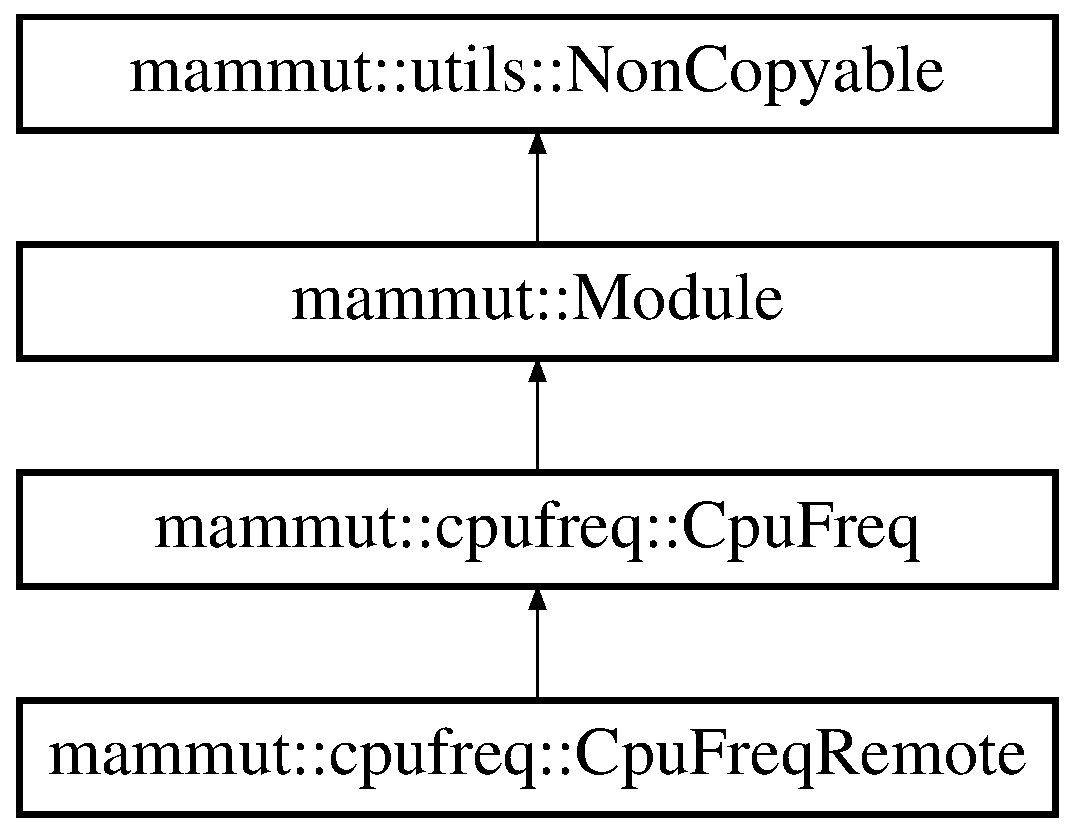
\includegraphics[height=4.000000cm]{classmammut_1_1cpufreq_1_1CpuFreqRemote}
\end{center}
\end{figure}
\subsection*{Public Member Functions}
\begin{DoxyCompactItemize}
\item 
\hypertarget{classmammut_1_1cpufreq_1_1CpuFreqRemote_a548db0c9f312e4bdaddf5804a94b25b9}{{\bfseries Cpu\-Freq\-Remote} (\hyperlink{classmammut_1_1Communicator}{Communicator} $\ast$const communicator)}\label{classmammut_1_1cpufreq_1_1CpuFreqRemote_a548db0c9f312e4bdaddf5804a94b25b9}

\item 
std\-::vector$<$ \hyperlink{classmammut_1_1cpufreq_1_1Domain}{Domain} $\ast$ $>$ \hyperlink{classmammut_1_1cpufreq_1_1CpuFreqRemote_a07b1ffad978a91b5179d339697ded144}{get\-Domains} () const 
\item 
bool \hyperlink{classmammut_1_1cpufreq_1_1CpuFreqRemote_a5def353551f4f9e50c62ae3367532e40}{is\-Boosting\-Supported} () const 
\item 
bool \hyperlink{classmammut_1_1cpufreq_1_1CpuFreqRemote_aa08948a1c885cc0ebac412d6734f6cbb}{is\-Boosting\-Enabled} () const 
\item 
void \hyperlink{classmammut_1_1cpufreq_1_1CpuFreqRemote_a230fbe7271cf8091411a065477498140}{enable\-Boosting} () const 
\item 
void \hyperlink{classmammut_1_1cpufreq_1_1CpuFreqRemote_ac48475824e7dbd675418dc95ac1bdd1e}{disable\-Boosting} () const 
\end{DoxyCompactItemize}
\subsection*{Additional Inherited Members}


\subsection{Member Function Documentation}
\hypertarget{classmammut_1_1cpufreq_1_1CpuFreqRemote_ac48475824e7dbd675418dc95ac1bdd1e}{\index{mammut\-::cpufreq\-::\-Cpu\-Freq\-Remote@{mammut\-::cpufreq\-::\-Cpu\-Freq\-Remote}!disable\-Boosting@{disable\-Boosting}}
\index{disable\-Boosting@{disable\-Boosting}!mammut::cpufreq::CpuFreqRemote@{mammut\-::cpufreq\-::\-Cpu\-Freq\-Remote}}
\subsubsection[{disable\-Boosting}]{\setlength{\rightskip}{0pt plus 5cm}void mammut\-::cpufreq\-::\-Cpu\-Freq\-Remote\-::disable\-Boosting (
\begin{DoxyParamCaption}
{}
\end{DoxyParamCaption}
) const\hspace{0.3cm}{\ttfamily [virtual]}}}\label{classmammut_1_1cpufreq_1_1CpuFreqRemote_ac48475824e7dbd675418dc95ac1bdd1e}
Disabled frequency boosting. 

Implements \hyperlink{classmammut_1_1cpufreq_1_1CpuFreq_a8abff63046f3b4ce5b992d4716fdabd1}{mammut\-::cpufreq\-::\-Cpu\-Freq}.

\hypertarget{classmammut_1_1cpufreq_1_1CpuFreqRemote_a230fbe7271cf8091411a065477498140}{\index{mammut\-::cpufreq\-::\-Cpu\-Freq\-Remote@{mammut\-::cpufreq\-::\-Cpu\-Freq\-Remote}!enable\-Boosting@{enable\-Boosting}}
\index{enable\-Boosting@{enable\-Boosting}!mammut::cpufreq::CpuFreqRemote@{mammut\-::cpufreq\-::\-Cpu\-Freq\-Remote}}
\subsubsection[{enable\-Boosting}]{\setlength{\rightskip}{0pt plus 5cm}void mammut\-::cpufreq\-::\-Cpu\-Freq\-Remote\-::enable\-Boosting (
\begin{DoxyParamCaption}
{}
\end{DoxyParamCaption}
) const\hspace{0.3cm}{\ttfamily [virtual]}}}\label{classmammut_1_1cpufreq_1_1CpuFreqRemote_a230fbe7271cf8091411a065477498140}
Enables frequency boosting. 

Implements \hyperlink{classmammut_1_1cpufreq_1_1CpuFreq_a53f6662c7cf58861d562266c95a61e8c}{mammut\-::cpufreq\-::\-Cpu\-Freq}.

\hypertarget{classmammut_1_1cpufreq_1_1CpuFreqRemote_a07b1ffad978a91b5179d339697ded144}{\index{mammut\-::cpufreq\-::\-Cpu\-Freq\-Remote@{mammut\-::cpufreq\-::\-Cpu\-Freq\-Remote}!get\-Domains@{get\-Domains}}
\index{get\-Domains@{get\-Domains}!mammut::cpufreq::CpuFreqRemote@{mammut\-::cpufreq\-::\-Cpu\-Freq\-Remote}}
\subsubsection[{get\-Domains}]{\setlength{\rightskip}{0pt plus 5cm}std\-::vector$<${\bf Domain}$\ast$$>$ mammut\-::cpufreq\-::\-Cpu\-Freq\-Remote\-::get\-Domains (
\begin{DoxyParamCaption}
{}
\end{DoxyParamCaption}
) const\hspace{0.3cm}{\ttfamily [virtual]}}}\label{classmammut_1_1cpufreq_1_1CpuFreqRemote_a07b1ffad978a91b5179d339697ded144}
Gets the domains division of the cores. \begin{DoxyReturn}{Returns}
A vector of domains. 
\end{DoxyReturn}


Implements \hyperlink{classmammut_1_1cpufreq_1_1CpuFreq_a2ff7cb9b384f506f17340089bba3ba99}{mammut\-::cpufreq\-::\-Cpu\-Freq}.

\hypertarget{classmammut_1_1cpufreq_1_1CpuFreqRemote_aa08948a1c885cc0ebac412d6734f6cbb}{\index{mammut\-::cpufreq\-::\-Cpu\-Freq\-Remote@{mammut\-::cpufreq\-::\-Cpu\-Freq\-Remote}!is\-Boosting\-Enabled@{is\-Boosting\-Enabled}}
\index{is\-Boosting\-Enabled@{is\-Boosting\-Enabled}!mammut::cpufreq::CpuFreqRemote@{mammut\-::cpufreq\-::\-Cpu\-Freq\-Remote}}
\subsubsection[{is\-Boosting\-Enabled}]{\setlength{\rightskip}{0pt plus 5cm}bool mammut\-::cpufreq\-::\-Cpu\-Freq\-Remote\-::is\-Boosting\-Enabled (
\begin{DoxyParamCaption}
{}
\end{DoxyParamCaption}
) const\hspace{0.3cm}{\ttfamily [virtual]}}}\label{classmammut_1_1cpufreq_1_1CpuFreqRemote_aa08948a1c885cc0ebac412d6734f6cbb}
Returns true if frequency boosting is enabled. \begin{DoxyReturn}{Returns}
True if frequency boosting is enabled, false otherwise. 
\end{DoxyReturn}


Implements \hyperlink{classmammut_1_1cpufreq_1_1CpuFreq_acc8da4a88e11b5e974a4877e2ff1ef95}{mammut\-::cpufreq\-::\-Cpu\-Freq}.

\hypertarget{classmammut_1_1cpufreq_1_1CpuFreqRemote_a5def353551f4f9e50c62ae3367532e40}{\index{mammut\-::cpufreq\-::\-Cpu\-Freq\-Remote@{mammut\-::cpufreq\-::\-Cpu\-Freq\-Remote}!is\-Boosting\-Supported@{is\-Boosting\-Supported}}
\index{is\-Boosting\-Supported@{is\-Boosting\-Supported}!mammut::cpufreq::CpuFreqRemote@{mammut\-::cpufreq\-::\-Cpu\-Freq\-Remote}}
\subsubsection[{is\-Boosting\-Supported}]{\setlength{\rightskip}{0pt plus 5cm}bool mammut\-::cpufreq\-::\-Cpu\-Freq\-Remote\-::is\-Boosting\-Supported (
\begin{DoxyParamCaption}
{}
\end{DoxyParamCaption}
) const\hspace{0.3cm}{\ttfamily [virtual]}}}\label{classmammut_1_1cpufreq_1_1CpuFreqRemote_a5def353551f4f9e50c62ae3367532e40}
Returns true if frequency boosting is supported. \begin{DoxyReturn}{Returns}
True if frequency boosting is supported, false otherwise. 
\end{DoxyReturn}


Implements \hyperlink{classmammut_1_1cpufreq_1_1CpuFreq_a93c7855b33a6794ddb8ba1aa0d4a5496}{mammut\-::cpufreq\-::\-Cpu\-Freq}.



The documentation for this class was generated from the following file\-:\begin{DoxyCompactItemize}
\item 
/home/daniele/\-Code/\-Mammut/mammut/cpufreq/cpufreq-\/remote.\-hpp\end{DoxyCompactItemize}

\hypertarget{classmammut_1_1topology_1_1CpuLinux}{\section{mammut\-:\-:topology\-:\-:Cpu\-Linux Class Reference}
\label{classmammut_1_1topology_1_1CpuLinux}\index{mammut\-::topology\-::\-Cpu\-Linux@{mammut\-::topology\-::\-Cpu\-Linux}}
}
Inheritance diagram for mammut\-:\-:topology\-:\-:Cpu\-Linux\-:\begin{figure}[H]
\begin{center}
\leavevmode
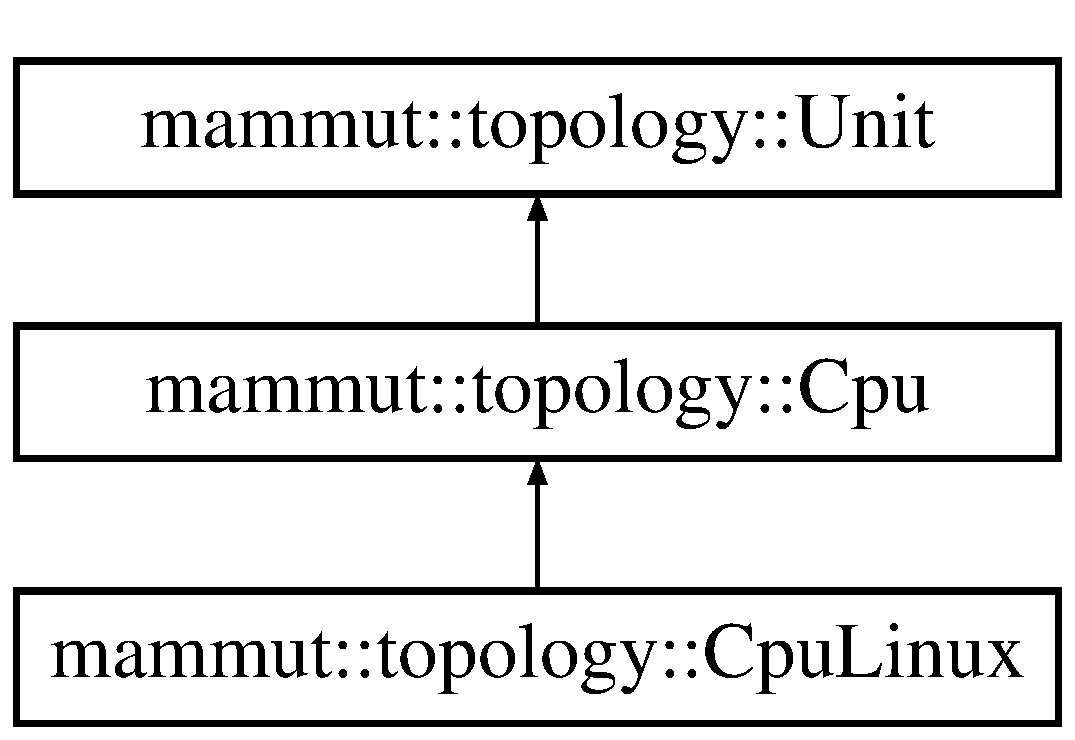
\includegraphics[height=3.000000cm]{classmammut_1_1topology_1_1CpuLinux}
\end{center}
\end{figure}
\subsection*{Public Member Functions}
\begin{DoxyCompactItemize}
\item 
\hypertarget{classmammut_1_1topology_1_1CpuLinux_a2cbd102ef72df0716ba11029e9bd4d8f}{{\bfseries Cpu\-Linux} (Cpu\-Id cpu\-Id, std\-::vector$<$ \hyperlink{classmammut_1_1topology_1_1PhysicalCore}{Physical\-Core} $\ast$ $>$ physical\-Cores)}\label{classmammut_1_1topology_1_1CpuLinux_a2cbd102ef72df0716ba11029e9bd4d8f}

\item 
std\-::string \hyperlink{classmammut_1_1topology_1_1CpuLinux_a95f8d7d4f1d8fc23a4e3c0a7b7879be1}{get\-Vendor\-Id} () const 
\item 
std\-::string \hyperlink{classmammut_1_1topology_1_1CpuLinux_af6d293f96505b4269d0e763588ec538f}{get\-Family} () const 
\item 
std\-::string \hyperlink{classmammut_1_1topology_1_1CpuLinux_ad1fe33a16052441fd0ed67734452b984}{get\-Model} () const 
\item 
void \hyperlink{classmammut_1_1topology_1_1CpuLinux_a428a9356fce899f82494f0973201f009}{maximize\-Utilization} () const 
\item 
void \hyperlink{classmammut_1_1topology_1_1CpuLinux_ae22825c9a86f221c3ffe9c456dfe96aa}{reset\-Utilization} () const 
\end{DoxyCompactItemize}
\subsection*{Additional Inherited Members}


\subsection{Member Function Documentation}
\hypertarget{classmammut_1_1topology_1_1CpuLinux_af6d293f96505b4269d0e763588ec538f}{\index{mammut\-::topology\-::\-Cpu\-Linux@{mammut\-::topology\-::\-Cpu\-Linux}!get\-Family@{get\-Family}}
\index{get\-Family@{get\-Family}!mammut::topology::CpuLinux@{mammut\-::topology\-::\-Cpu\-Linux}}
\subsubsection[{get\-Family}]{\setlength{\rightskip}{0pt plus 5cm}std\-::string mammut\-::topology\-::\-Cpu\-Linux\-::get\-Family (
\begin{DoxyParamCaption}
{}
\end{DoxyParamCaption}
) const\hspace{0.3cm}{\ttfamily [virtual]}}}\label{classmammut_1_1topology_1_1CpuLinux_af6d293f96505b4269d0e763588ec538f}
Returns the family of this \hyperlink{classmammut_1_1topology_1_1Cpu}{Cpu}. \begin{DoxyReturn}{Returns}
The family of this \hyperlink{classmammut_1_1topology_1_1Cpu}{Cpu}. 
\end{DoxyReturn}


Implements \hyperlink{classmammut_1_1topology_1_1Cpu_a14f0984b504c0c207250829728193f8c}{mammut\-::topology\-::\-Cpu}.

\hypertarget{classmammut_1_1topology_1_1CpuLinux_ad1fe33a16052441fd0ed67734452b984}{\index{mammut\-::topology\-::\-Cpu\-Linux@{mammut\-::topology\-::\-Cpu\-Linux}!get\-Model@{get\-Model}}
\index{get\-Model@{get\-Model}!mammut::topology::CpuLinux@{mammut\-::topology\-::\-Cpu\-Linux}}
\subsubsection[{get\-Model}]{\setlength{\rightskip}{0pt plus 5cm}std\-::string mammut\-::topology\-::\-Cpu\-Linux\-::get\-Model (
\begin{DoxyParamCaption}
{}
\end{DoxyParamCaption}
) const\hspace{0.3cm}{\ttfamily [virtual]}}}\label{classmammut_1_1topology_1_1CpuLinux_ad1fe33a16052441fd0ed67734452b984}
Returns the model of this \hyperlink{classmammut_1_1topology_1_1Cpu}{Cpu}. \begin{DoxyReturn}{Returns}
The model of this \hyperlink{classmammut_1_1topology_1_1Cpu}{Cpu}. 
\end{DoxyReturn}


Implements \hyperlink{classmammut_1_1topology_1_1Cpu_a6e98555afbc9d4985acc4ec30fbc5d96}{mammut\-::topology\-::\-Cpu}.

\hypertarget{classmammut_1_1topology_1_1CpuLinux_a95f8d7d4f1d8fc23a4e3c0a7b7879be1}{\index{mammut\-::topology\-::\-Cpu\-Linux@{mammut\-::topology\-::\-Cpu\-Linux}!get\-Vendor\-Id@{get\-Vendor\-Id}}
\index{get\-Vendor\-Id@{get\-Vendor\-Id}!mammut::topology::CpuLinux@{mammut\-::topology\-::\-Cpu\-Linux}}
\subsubsection[{get\-Vendor\-Id}]{\setlength{\rightskip}{0pt plus 5cm}std\-::string mammut\-::topology\-::\-Cpu\-Linux\-::get\-Vendor\-Id (
\begin{DoxyParamCaption}
{}
\end{DoxyParamCaption}
) const\hspace{0.3cm}{\ttfamily [virtual]}}}\label{classmammut_1_1topology_1_1CpuLinux_a95f8d7d4f1d8fc23a4e3c0a7b7879be1}
Returns the vendor id of this \hyperlink{classmammut_1_1topology_1_1Cpu}{Cpu}. \begin{DoxyReturn}{Returns}
The vendor id of this \hyperlink{classmammut_1_1topology_1_1Cpu}{Cpu}. 
\end{DoxyReturn}


Implements \hyperlink{classmammut_1_1topology_1_1Cpu_a7b1fcfcc8df09588832ca1dc6351e6f1}{mammut\-::topology\-::\-Cpu}.

\hypertarget{classmammut_1_1topology_1_1CpuLinux_a428a9356fce899f82494f0973201f009}{\index{mammut\-::topology\-::\-Cpu\-Linux@{mammut\-::topology\-::\-Cpu\-Linux}!maximize\-Utilization@{maximize\-Utilization}}
\index{maximize\-Utilization@{maximize\-Utilization}!mammut::topology::CpuLinux@{mammut\-::topology\-::\-Cpu\-Linux}}
\subsubsection[{maximize\-Utilization}]{\setlength{\rightskip}{0pt plus 5cm}void mammut\-::topology\-::\-Cpu\-Linux\-::maximize\-Utilization (
\begin{DoxyParamCaption}
{}
\end{DoxyParamCaption}
) const\hspace{0.3cm}{\ttfamily [virtual]}}}\label{classmammut_1_1topology_1_1CpuLinux_a428a9356fce899f82494f0973201f009}
Bring the utilization of this C\-P\-U to 100\% until \hyperlink{classmammut_1_1topology_1_1CpuLinux_ae22825c9a86f221c3ffe9c456dfe96aa}{reset\-Utilization()} is called. 

Implements \hyperlink{classmammut_1_1topology_1_1Cpu_a249829ade28b8fffcda1d2666cf68997}{mammut\-::topology\-::\-Cpu}.

\hypertarget{classmammut_1_1topology_1_1CpuLinux_ae22825c9a86f221c3ffe9c456dfe96aa}{\index{mammut\-::topology\-::\-Cpu\-Linux@{mammut\-::topology\-::\-Cpu\-Linux}!reset\-Utilization@{reset\-Utilization}}
\index{reset\-Utilization@{reset\-Utilization}!mammut::topology::CpuLinux@{mammut\-::topology\-::\-Cpu\-Linux}}
\subsubsection[{reset\-Utilization}]{\setlength{\rightskip}{0pt plus 5cm}void mammut\-::topology\-::\-Cpu\-Linux\-::reset\-Utilization (
\begin{DoxyParamCaption}
{}
\end{DoxyParamCaption}
) const\hspace{0.3cm}{\ttfamily [virtual]}}}\label{classmammut_1_1topology_1_1CpuLinux_ae22825c9a86f221c3ffe9c456dfe96aa}
Resets the utilization of this C\-P\-U. 

Implements \hyperlink{classmammut_1_1topology_1_1Cpu_a3eea41d7ad6200d83301102f23944de5}{mammut\-::topology\-::\-Cpu}.



The documentation for this class was generated from the following files\-:\begin{DoxyCompactItemize}
\item 
/home/daniele/\-Code/\-Mammut/mammut/topology/topology-\/linux.\-hpp\item 
/home/daniele/\-Code/\-Mammut/mammut/topology/topology-\/linux.\-cpp\end{DoxyCompactItemize}

\hypertarget{classmammut_1_1topology_1_1CpuRemote}{\section{mammut\-:\-:topology\-:\-:Cpu\-Remote Class Reference}
\label{classmammut_1_1topology_1_1CpuRemote}\index{mammut\-::topology\-::\-Cpu\-Remote@{mammut\-::topology\-::\-Cpu\-Remote}}
}
Inheritance diagram for mammut\-:\-:topology\-:\-:Cpu\-Remote\-:\begin{figure}[H]
\begin{center}
\leavevmode
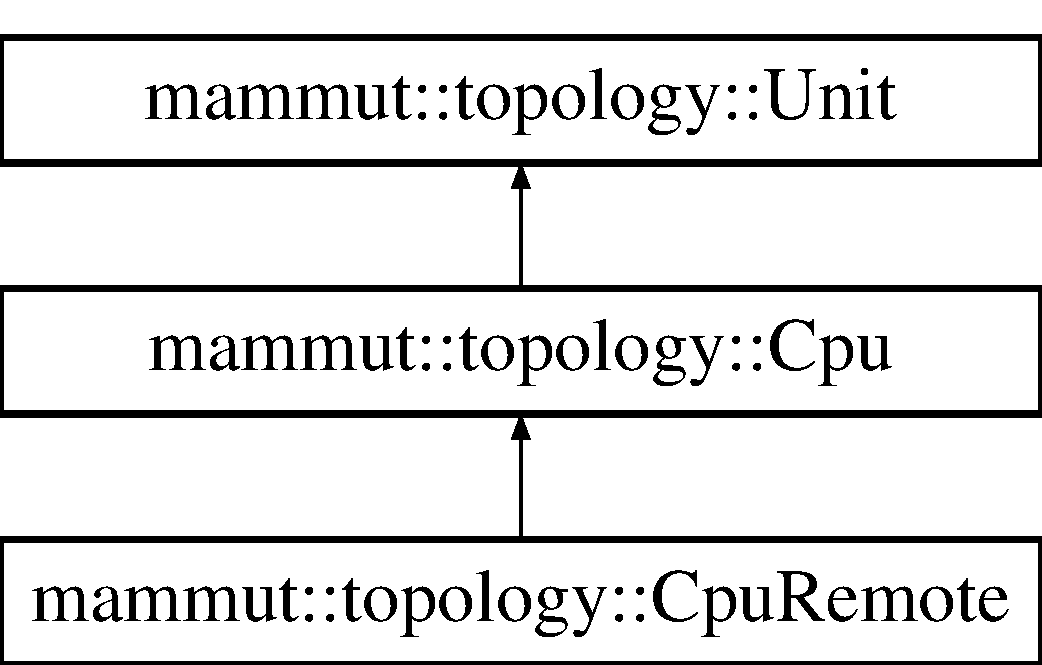
\includegraphics[height=3.000000cm]{classmammut_1_1topology_1_1CpuRemote}
\end{center}
\end{figure}
\subsection*{Public Member Functions}
\begin{DoxyCompactItemize}
\item 
\hypertarget{classmammut_1_1topology_1_1CpuRemote_abba5a5ebf1457ade6bfb6d5485f51e2f}{{\bfseries Cpu\-Remote} (\hyperlink{classmammut_1_1Communicator}{Communicator} $\ast$const communicator, Cpu\-Id cpu\-Id, std\-::vector$<$ \hyperlink{classmammut_1_1topology_1_1PhysicalCore}{Physical\-Core} $\ast$ $>$ physical\-Cores)}\label{classmammut_1_1topology_1_1CpuRemote_abba5a5ebf1457ade6bfb6d5485f51e2f}

\item 
std\-::string \hyperlink{classmammut_1_1topology_1_1CpuRemote_a3a49baf79550998a4d8782587cb27704}{get\-Vendor\-Id} () const 
\item 
std\-::string \hyperlink{classmammut_1_1topology_1_1CpuRemote_aacd6e5bee5d9b348220749efc614b6d1}{get\-Family} () const 
\item 
std\-::string \hyperlink{classmammut_1_1topology_1_1CpuRemote_a7d57ba15fa3db7f444c5757c5da93bdb}{get\-Model} () const 
\item 
void \hyperlink{classmammut_1_1topology_1_1CpuRemote_a1f25bdc6f2b049a831a03ba702699626}{maximize\-Utilization} () const 
\item 
void \hyperlink{classmammut_1_1topology_1_1CpuRemote_a689af84ac46ab57081fc4fa47c9992b6}{reset\-Utilization} () const 
\end{DoxyCompactItemize}
\subsection*{Additional Inherited Members}


\subsection{Member Function Documentation}
\hypertarget{classmammut_1_1topology_1_1CpuRemote_aacd6e5bee5d9b348220749efc614b6d1}{\index{mammut\-::topology\-::\-Cpu\-Remote@{mammut\-::topology\-::\-Cpu\-Remote}!get\-Family@{get\-Family}}
\index{get\-Family@{get\-Family}!mammut::topology::CpuRemote@{mammut\-::topology\-::\-Cpu\-Remote}}
\subsubsection[{get\-Family}]{\setlength{\rightskip}{0pt plus 5cm}std\-::string mammut\-::topology\-::\-Cpu\-Remote\-::get\-Family (
\begin{DoxyParamCaption}
{}
\end{DoxyParamCaption}
) const\hspace{0.3cm}{\ttfamily [virtual]}}}\label{classmammut_1_1topology_1_1CpuRemote_aacd6e5bee5d9b348220749efc614b6d1}
Returns the family of this \hyperlink{classmammut_1_1topology_1_1Cpu}{Cpu}. \begin{DoxyReturn}{Returns}
The family of this \hyperlink{classmammut_1_1topology_1_1Cpu}{Cpu}. 
\end{DoxyReturn}


Implements \hyperlink{classmammut_1_1topology_1_1Cpu_a14f0984b504c0c207250829728193f8c}{mammut\-::topology\-::\-Cpu}.

\hypertarget{classmammut_1_1topology_1_1CpuRemote_a7d57ba15fa3db7f444c5757c5da93bdb}{\index{mammut\-::topology\-::\-Cpu\-Remote@{mammut\-::topology\-::\-Cpu\-Remote}!get\-Model@{get\-Model}}
\index{get\-Model@{get\-Model}!mammut::topology::CpuRemote@{mammut\-::topology\-::\-Cpu\-Remote}}
\subsubsection[{get\-Model}]{\setlength{\rightskip}{0pt plus 5cm}std\-::string mammut\-::topology\-::\-Cpu\-Remote\-::get\-Model (
\begin{DoxyParamCaption}
{}
\end{DoxyParamCaption}
) const\hspace{0.3cm}{\ttfamily [virtual]}}}\label{classmammut_1_1topology_1_1CpuRemote_a7d57ba15fa3db7f444c5757c5da93bdb}
Returns the model of this \hyperlink{classmammut_1_1topology_1_1Cpu}{Cpu}. \begin{DoxyReturn}{Returns}
The model of this \hyperlink{classmammut_1_1topology_1_1Cpu}{Cpu}. 
\end{DoxyReturn}


Implements \hyperlink{classmammut_1_1topology_1_1Cpu_a6e98555afbc9d4985acc4ec30fbc5d96}{mammut\-::topology\-::\-Cpu}.

\hypertarget{classmammut_1_1topology_1_1CpuRemote_a3a49baf79550998a4d8782587cb27704}{\index{mammut\-::topology\-::\-Cpu\-Remote@{mammut\-::topology\-::\-Cpu\-Remote}!get\-Vendor\-Id@{get\-Vendor\-Id}}
\index{get\-Vendor\-Id@{get\-Vendor\-Id}!mammut::topology::CpuRemote@{mammut\-::topology\-::\-Cpu\-Remote}}
\subsubsection[{get\-Vendor\-Id}]{\setlength{\rightskip}{0pt plus 5cm}std\-::string mammut\-::topology\-::\-Cpu\-Remote\-::get\-Vendor\-Id (
\begin{DoxyParamCaption}
{}
\end{DoxyParamCaption}
) const\hspace{0.3cm}{\ttfamily [virtual]}}}\label{classmammut_1_1topology_1_1CpuRemote_a3a49baf79550998a4d8782587cb27704}
Returns the vendor id of this \hyperlink{classmammut_1_1topology_1_1Cpu}{Cpu}. \begin{DoxyReturn}{Returns}
The vendor id of this \hyperlink{classmammut_1_1topology_1_1Cpu}{Cpu}. 
\end{DoxyReturn}


Implements \hyperlink{classmammut_1_1topology_1_1Cpu_a7b1fcfcc8df09588832ca1dc6351e6f1}{mammut\-::topology\-::\-Cpu}.

\hypertarget{classmammut_1_1topology_1_1CpuRemote_a1f25bdc6f2b049a831a03ba702699626}{\index{mammut\-::topology\-::\-Cpu\-Remote@{mammut\-::topology\-::\-Cpu\-Remote}!maximize\-Utilization@{maximize\-Utilization}}
\index{maximize\-Utilization@{maximize\-Utilization}!mammut::topology::CpuRemote@{mammut\-::topology\-::\-Cpu\-Remote}}
\subsubsection[{maximize\-Utilization}]{\setlength{\rightskip}{0pt plus 5cm}void mammut\-::topology\-::\-Cpu\-Remote\-::maximize\-Utilization (
\begin{DoxyParamCaption}
{}
\end{DoxyParamCaption}
) const\hspace{0.3cm}{\ttfamily [virtual]}}}\label{classmammut_1_1topology_1_1CpuRemote_a1f25bdc6f2b049a831a03ba702699626}
Bring the utilization of this C\-P\-U to 100\% until \hyperlink{classmammut_1_1topology_1_1CpuRemote_a689af84ac46ab57081fc4fa47c9992b6}{reset\-Utilization()} is called. 

Implements \hyperlink{classmammut_1_1topology_1_1Cpu_a249829ade28b8fffcda1d2666cf68997}{mammut\-::topology\-::\-Cpu}.

\hypertarget{classmammut_1_1topology_1_1CpuRemote_a689af84ac46ab57081fc4fa47c9992b6}{\index{mammut\-::topology\-::\-Cpu\-Remote@{mammut\-::topology\-::\-Cpu\-Remote}!reset\-Utilization@{reset\-Utilization}}
\index{reset\-Utilization@{reset\-Utilization}!mammut::topology::CpuRemote@{mammut\-::topology\-::\-Cpu\-Remote}}
\subsubsection[{reset\-Utilization}]{\setlength{\rightskip}{0pt plus 5cm}void mammut\-::topology\-::\-Cpu\-Remote\-::reset\-Utilization (
\begin{DoxyParamCaption}
{}
\end{DoxyParamCaption}
) const\hspace{0.3cm}{\ttfamily [virtual]}}}\label{classmammut_1_1topology_1_1CpuRemote_a689af84ac46ab57081fc4fa47c9992b6}
Resets the utilization of this C\-P\-U. 

Implements \hyperlink{classmammut_1_1topology_1_1Cpu_a3eea41d7ad6200d83301102f23944de5}{mammut\-::topology\-::\-Cpu}.



The documentation for this class was generated from the following file\-:\begin{DoxyCompactItemize}
\item 
/home/daniele/\-Code/\-Mammut/mammut/topology/topology-\/remote.\-hpp\end{DoxyCompactItemize}

\hypertarget{classmammut_1_1cpufreq_1_1Domain}{\section{mammut\-:\-:cpufreq\-:\-:Domain Class Reference}
\label{classmammut_1_1cpufreq_1_1Domain}\index{mammut\-::cpufreq\-::\-Domain@{mammut\-::cpufreq\-::\-Domain}}
}


{\ttfamily \#include $<$cpufreq.\-hpp$>$}

Inheritance diagram for mammut\-:\-:cpufreq\-:\-:Domain\-:\begin{figure}[H]
\begin{center}
\leavevmode
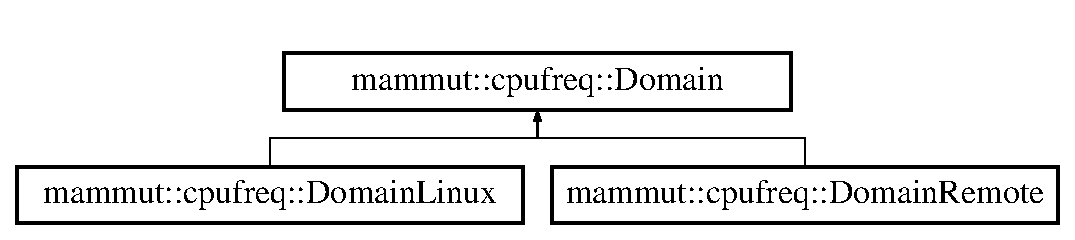
\includegraphics[height=2.000000cm]{classmammut_1_1cpufreq_1_1Domain}
\end{center}
\end{figure}
\subsection*{Public Member Functions}
\begin{DoxyCompactItemize}
\item 
std\-::vector\\*
$<$ \hyperlink{classmammut_1_1topology_1_1VirtualCore}{topology\-::\-Virtual\-Core} $\ast$ $>$ \hyperlink{classmammut_1_1cpufreq_1_1Domain_aadbd6c6cd1d9c9abd6ac0100623b6f55}{get\-Virtual\-Cores} () const 
\item 
std\-::vector\\*
$<$ topology\-::\-Virtual\-Core\-Id $>$ \hyperlink{classmammut_1_1cpufreq_1_1Domain_a1952a345d43f937eb677170c488beeaf}{get\-Virtual\-Cores\-Identifiers} () const 
\item 
bool \hyperlink{classmammut_1_1cpufreq_1_1Domain_a48f7f709c4de763ae757cf792ef20f6c}{contains} (const \hyperlink{classmammut_1_1topology_1_1VirtualCore}{topology\-::\-Virtual\-Core} $\ast$virtual\-Core) const 
\item 
Domain\-Id \hyperlink{classmammut_1_1cpufreq_1_1Domain_a9e704e1fa89206f5238e8cc12eb1c3d0}{get\-Id} () const 
\item 
\hyperlink{structmammut_1_1cpufreq_1_1RollbackPoint}{Rollback\-Point} \hyperlink{classmammut_1_1cpufreq_1_1Domain_a7ce84c12b87b4aabb14686c38f64feae}{get\-Rollback\-Point} () const 
\item 
void \hyperlink{classmammut_1_1cpufreq_1_1Domain_abcd5b9b96fc708cd5456e8856a1b6f8a}{rollback} (const \hyperlink{structmammut_1_1cpufreq_1_1RollbackPoint}{Rollback\-Point} \&rollback\-Point) const 
\item 
virtual std\-::vector$<$ Frequency $>$ \hyperlink{classmammut_1_1cpufreq_1_1Domain_a77f57f47e688a3aaae168a2f9e8dc062}{get\-Available\-Frequencies} () const =0
\item 
virtual std\-::vector$<$ Governor $>$ \hyperlink{classmammut_1_1cpufreq_1_1Domain_ab72f441a05214166a07c4ece122f02c6}{get\-Available\-Governors} () const =0
\item 
bool \hyperlink{classmammut_1_1cpufreq_1_1Domain_a0e4d5b325d00884509f3c1f34d2525a3}{is\-Governor\-Available} (Governor governor) const 
\item 
virtual Frequency \hyperlink{classmammut_1_1cpufreq_1_1Domain_a915d7a5e4da2fe377c9805e86820ac3e}{get\-Current\-Frequency} () const =0
\item 
virtual Frequency \hyperlink{classmammut_1_1cpufreq_1_1Domain_abb5e1908d54a2af862e78b03a1a85af4}{get\-Current\-Frequency\-Userspace} () const =0
\item 
virtual bool \hyperlink{classmammut_1_1cpufreq_1_1Domain_a6f97e04fa138bbb6b478c8a7338b4116}{set\-Frequency\-Userspace} (Frequency frequency) const =0
\item 
bool \hyperlink{classmammut_1_1cpufreq_1_1Domain_ab4a7179ca9f0b0ed372579dacc93c196}{set\-Highest\-Frequency\-Userspace} () const 
\item 
bool \hyperlink{classmammut_1_1cpufreq_1_1Domain_ae473572f0b075de12bcf063b49815086}{set\-Lowest\-Frequency\-Userspace} () const 
\item 
virtual Governor \hyperlink{classmammut_1_1cpufreq_1_1Domain_a938483ec97ed59d0559758a1a467dc62}{get\-Current\-Governor} () const =0
\item 
virtual bool \hyperlink{classmammut_1_1cpufreq_1_1Domain_a48cb064376b9b663e5a134a61b5780bd}{set\-Governor} (Governor governor) const =0
\item 
virtual void \hyperlink{classmammut_1_1cpufreq_1_1Domain_a652712c9192a755fb2bc6b58076eccb8}{get\-Hardware\-Frequency\-Bounds} (Frequency \&lower\-Bound, Frequency \&upper\-Bound) const =0
\item 
virtual bool \hyperlink{classmammut_1_1cpufreq_1_1Domain_af95ae412f43dfbf60a77715ef4684c0f}{get\-Current\-Governor\-Bounds} (Frequency \&lower\-Bound, Frequency \&upper\-Bound) const =0
\item 
virtual bool \hyperlink{classmammut_1_1cpufreq_1_1Domain_a45a0a69b4957937c921e723bbcf6cf04}{set\-Governor\-Bounds} (Frequency lower\-Bound, Frequency upper\-Bound) const =0
\item 
virtual int \hyperlink{classmammut_1_1cpufreq_1_1Domain_a0c7d34dc9ee1e5eb57200a127ae9f183}{get\-Transition\-Latency} () const =0
\item 
virtual Voltage \hyperlink{classmammut_1_1cpufreq_1_1Domain_acd823bdc2f011c042dbb272c4d63df3c}{get\-Current\-Voltage} () const =0
\item 
virtual Voltage\-Table \hyperlink{classmammut_1_1cpufreq_1_1Domain_ad0b11fad2e36e45d6028de662df63ba8}{get\-Voltage\-Table} (bool only\-Physical\-Cores=true) const =0
\item 
virtual Voltage\-Table \hyperlink{classmammut_1_1cpufreq_1_1Domain_a4442dfd2b7d52a95ad4bdf3e99185bf3}{get\-Voltage\-Table} (uint num\-Virtual\-Cores, bool only\-Physical\-Cores) const =0
\end{DoxyCompactItemize}
\subsection*{Protected Member Functions}
\begin{DoxyCompactItemize}
\item 
\hypertarget{classmammut_1_1cpufreq_1_1Domain_a7c5ae0a8f2109fa0adfcf891e6696b0f}{{\bfseries Domain} (Domain\-Id domain\-Identifier, std\-::vector$<$ \hyperlink{classmammut_1_1topology_1_1VirtualCore}{topology\-::\-Virtual\-Core} $\ast$ $>$ virtual\-Cores)}\label{classmammut_1_1cpufreq_1_1Domain_a7c5ae0a8f2109fa0adfcf891e6696b0f}

\end{DoxyCompactItemize}
\subsection*{Protected Attributes}
\begin{DoxyCompactItemize}
\item 
\hypertarget{classmammut_1_1cpufreq_1_1Domain_ae71a3d8c629d75fab1a6cf313e445d3c}{const std\-::vector\\*
$<$ \hyperlink{classmammut_1_1topology_1_1VirtualCore}{topology\-::\-Virtual\-Core} $\ast$ $>$ {\bfseries \-\_\-virtual\-Cores}}\label{classmammut_1_1cpufreq_1_1Domain_ae71a3d8c629d75fab1a6cf313e445d3c}

\end{DoxyCompactItemize}


\subsection{Detailed Description}
Represents a set of virtual cores related between each other. When the frequency/governor changes for one core in the domain, it changes for the other cores in the same domain too. 

\subsection{Member Function Documentation}
\hypertarget{classmammut_1_1cpufreq_1_1Domain_a48f7f709c4de763ae757cf792ef20f6c}{\index{mammut\-::cpufreq\-::\-Domain@{mammut\-::cpufreq\-::\-Domain}!contains@{contains}}
\index{contains@{contains}!mammut::cpufreq::Domain@{mammut\-::cpufreq\-::\-Domain}}
\subsubsection[{contains}]{\setlength{\rightskip}{0pt plus 5cm}bool mammut\-::cpufreq\-::\-Domain\-::contains (
\begin{DoxyParamCaption}
\item[{const {\bf topology\-::\-Virtual\-Core} $\ast$}]{virtual\-Core}
\end{DoxyParamCaption}
) const}}\label{classmammut_1_1cpufreq_1_1Domain_a48f7f709c4de763ae757cf792ef20f6c}
Checks if this domain contains a specific virtual core. 
\begin{DoxyParams}{Parameters}
{\em virtual\-Core} & The virtual core. \\
\hline
\end{DoxyParams}
\begin{DoxyReturn}{Returns}
true if this domain contains the virtual core, false otherwise. 
\end{DoxyReturn}
\hypertarget{classmammut_1_1cpufreq_1_1Domain_a77f57f47e688a3aaae168a2f9e8dc062}{\index{mammut\-::cpufreq\-::\-Domain@{mammut\-::cpufreq\-::\-Domain}!get\-Available\-Frequencies@{get\-Available\-Frequencies}}
\index{get\-Available\-Frequencies@{get\-Available\-Frequencies}!mammut::cpufreq::Domain@{mammut\-::cpufreq\-::\-Domain}}
\subsubsection[{get\-Available\-Frequencies}]{\setlength{\rightskip}{0pt plus 5cm}virtual std\-::vector$<$Frequency$>$ mammut\-::cpufreq\-::\-Domain\-::get\-Available\-Frequencies (
\begin{DoxyParamCaption}
{}
\end{DoxyParamCaption}
) const\hspace{0.3cm}{\ttfamily [pure virtual]}}}\label{classmammut_1_1cpufreq_1_1Domain_a77f57f47e688a3aaae168a2f9e8dc062}
Gets the frequency steps (in K\-Hz) available (sorted from lowest to highest). \begin{DoxyReturn}{Returns}
The frequency steps (in K\-Hz) available (sorted from lowest to highest). 
\end{DoxyReturn}


Implemented in \hyperlink{classmammut_1_1cpufreq_1_1DomainLinux_a842b3b21fb5fc87c65368dc48cbc02af}{mammut\-::cpufreq\-::\-Domain\-Linux}, and \hyperlink{classmammut_1_1cpufreq_1_1DomainRemote_a07132aa88d0c49d2f48a01e47604ae39}{mammut\-::cpufreq\-::\-Domain\-Remote}.

\hypertarget{classmammut_1_1cpufreq_1_1Domain_ab72f441a05214166a07c4ece122f02c6}{\index{mammut\-::cpufreq\-::\-Domain@{mammut\-::cpufreq\-::\-Domain}!get\-Available\-Governors@{get\-Available\-Governors}}
\index{get\-Available\-Governors@{get\-Available\-Governors}!mammut::cpufreq::Domain@{mammut\-::cpufreq\-::\-Domain}}
\subsubsection[{get\-Available\-Governors}]{\setlength{\rightskip}{0pt plus 5cm}virtual std\-::vector$<$Governor$>$ mammut\-::cpufreq\-::\-Domain\-::get\-Available\-Governors (
\begin{DoxyParamCaption}
{}
\end{DoxyParamCaption}
) const\hspace{0.3cm}{\ttfamily [pure virtual]}}}\label{classmammut_1_1cpufreq_1_1Domain_ab72f441a05214166a07c4ece122f02c6}
Gets the governors available. \begin{DoxyReturn}{Returns}
The governors available. 
\end{DoxyReturn}


Implemented in \hyperlink{classmammut_1_1cpufreq_1_1DomainLinux_a2596e269900a9567a02cf10b14407bb4}{mammut\-::cpufreq\-::\-Domain\-Linux}, and \hyperlink{classmammut_1_1cpufreq_1_1DomainRemote_a125ba0d251841a14853fb9830564fba8}{mammut\-::cpufreq\-::\-Domain\-Remote}.

\hypertarget{classmammut_1_1cpufreq_1_1Domain_a915d7a5e4da2fe377c9805e86820ac3e}{\index{mammut\-::cpufreq\-::\-Domain@{mammut\-::cpufreq\-::\-Domain}!get\-Current\-Frequency@{get\-Current\-Frequency}}
\index{get\-Current\-Frequency@{get\-Current\-Frequency}!mammut::cpufreq::Domain@{mammut\-::cpufreq\-::\-Domain}}
\subsubsection[{get\-Current\-Frequency}]{\setlength{\rightskip}{0pt plus 5cm}virtual Frequency mammut\-::cpufreq\-::\-Domain\-::get\-Current\-Frequency (
\begin{DoxyParamCaption}
{}
\end{DoxyParamCaption}
) const\hspace{0.3cm}{\ttfamily [pure virtual]}}}\label{classmammut_1_1cpufreq_1_1Domain_a915d7a5e4da2fe377c9805e86820ac3e}
Gets the current frequency. \begin{DoxyReturn}{Returns}
The current frequency. 
\end{DoxyReturn}


Implemented in \hyperlink{classmammut_1_1cpufreq_1_1DomainLinux_a31cda10038615a5d98fdf38a67a4682a}{mammut\-::cpufreq\-::\-Domain\-Linux}, and \hyperlink{classmammut_1_1cpufreq_1_1DomainRemote_a080d7be95c68f1dc57510a1fe4765f65}{mammut\-::cpufreq\-::\-Domain\-Remote}.

\hypertarget{classmammut_1_1cpufreq_1_1Domain_abb5e1908d54a2af862e78b03a1a85af4}{\index{mammut\-::cpufreq\-::\-Domain@{mammut\-::cpufreq\-::\-Domain}!get\-Current\-Frequency\-Userspace@{get\-Current\-Frequency\-Userspace}}
\index{get\-Current\-Frequency\-Userspace@{get\-Current\-Frequency\-Userspace}!mammut::cpufreq::Domain@{mammut\-::cpufreq\-::\-Domain}}
\subsubsection[{get\-Current\-Frequency\-Userspace}]{\setlength{\rightskip}{0pt plus 5cm}virtual Frequency mammut\-::cpufreq\-::\-Domain\-::get\-Current\-Frequency\-Userspace (
\begin{DoxyParamCaption}
{}
\end{DoxyParamCaption}
) const\hspace{0.3cm}{\ttfamily [pure virtual]}}}\label{classmammut_1_1cpufreq_1_1Domain_abb5e1908d54a2af862e78b03a1a85af4}
Gets the current frequency set by userspace governor. \begin{DoxyReturn}{Returns}
The current frequency if the current governor is userspace, a meaningless value otherwise. 
\end{DoxyReturn}


Implemented in \hyperlink{classmammut_1_1cpufreq_1_1DomainLinux_a22d59973df8f67d8bec1d50e9391cda6}{mammut\-::cpufreq\-::\-Domain\-Linux}, and \hyperlink{classmammut_1_1cpufreq_1_1DomainRemote_a0202e17b3b2a9ff30b711c5157ec9a86}{mammut\-::cpufreq\-::\-Domain\-Remote}.

\hypertarget{classmammut_1_1cpufreq_1_1Domain_a938483ec97ed59d0559758a1a467dc62}{\index{mammut\-::cpufreq\-::\-Domain@{mammut\-::cpufreq\-::\-Domain}!get\-Current\-Governor@{get\-Current\-Governor}}
\index{get\-Current\-Governor@{get\-Current\-Governor}!mammut::cpufreq::Domain@{mammut\-::cpufreq\-::\-Domain}}
\subsubsection[{get\-Current\-Governor}]{\setlength{\rightskip}{0pt plus 5cm}virtual Governor mammut\-::cpufreq\-::\-Domain\-::get\-Current\-Governor (
\begin{DoxyParamCaption}
{}
\end{DoxyParamCaption}
) const\hspace{0.3cm}{\ttfamily [pure virtual]}}}\label{classmammut_1_1cpufreq_1_1Domain_a938483ec97ed59d0559758a1a467dc62}
Gets the current governor. \begin{DoxyReturn}{Returns}
The current governor. 
\end{DoxyReturn}


Implemented in \hyperlink{classmammut_1_1cpufreq_1_1DomainLinux_ab8873a08cc11c89a6119ad87402d130d}{mammut\-::cpufreq\-::\-Domain\-Linux}, and \hyperlink{classmammut_1_1cpufreq_1_1DomainRemote_a44628a8aa9d605e683c3273ddbe549b7}{mammut\-::cpufreq\-::\-Domain\-Remote}.

\hypertarget{classmammut_1_1cpufreq_1_1Domain_af95ae412f43dfbf60a77715ef4684c0f}{\index{mammut\-::cpufreq\-::\-Domain@{mammut\-::cpufreq\-::\-Domain}!get\-Current\-Governor\-Bounds@{get\-Current\-Governor\-Bounds}}
\index{get\-Current\-Governor\-Bounds@{get\-Current\-Governor\-Bounds}!mammut::cpufreq::Domain@{mammut\-::cpufreq\-::\-Domain}}
\subsubsection[{get\-Current\-Governor\-Bounds}]{\setlength{\rightskip}{0pt plus 5cm}virtual bool mammut\-::cpufreq\-::\-Domain\-::get\-Current\-Governor\-Bounds (
\begin{DoxyParamCaption}
\item[{Frequency \&}]{lower\-Bound, }
\item[{Frequency \&}]{upper\-Bound}
\end{DoxyParamCaption}
) const\hspace{0.3cm}{\ttfamily [pure virtual]}}}\label{classmammut_1_1cpufreq_1_1Domain_af95ae412f43dfbf60a77715ef4684c0f}
Gets the current frequency bounds for the governor. 
\begin{DoxyParams}{Parameters}
{\em lower\-Bound} & The current frequency lower bound (specified in k\-H\-Z). \\
\hline
{\em upper\-Bound} & The current frequency upper bound (specified in k\-H\-Z). \\
\hline
\end{DoxyParams}
\begin{DoxyReturn}{Returns}
true if the governor is not userspace, false otherwise. 
\end{DoxyReturn}


Implemented in \hyperlink{classmammut_1_1cpufreq_1_1DomainLinux_ae84e936d5175b72112ed70a99971d6ae}{mammut\-::cpufreq\-::\-Domain\-Linux}, and \hyperlink{classmammut_1_1cpufreq_1_1DomainRemote_a351e9fc310205750a81417b5d5e278e0}{mammut\-::cpufreq\-::\-Domain\-Remote}.

\hypertarget{classmammut_1_1cpufreq_1_1Domain_acd823bdc2f011c042dbb272c4d63df3c}{\index{mammut\-::cpufreq\-::\-Domain@{mammut\-::cpufreq\-::\-Domain}!get\-Current\-Voltage@{get\-Current\-Voltage}}
\index{get\-Current\-Voltage@{get\-Current\-Voltage}!mammut::cpufreq::Domain@{mammut\-::cpufreq\-::\-Domain}}
\subsubsection[{get\-Current\-Voltage}]{\setlength{\rightskip}{0pt plus 5cm}virtual Voltage mammut\-::cpufreq\-::\-Domain\-::get\-Current\-Voltage (
\begin{DoxyParamCaption}
{}
\end{DoxyParamCaption}
) const\hspace{0.3cm}{\ttfamily [pure virtual]}}}\label{classmammut_1_1cpufreq_1_1Domain_acd823bdc2f011c042dbb272c4d63df3c}
Returns the current voltage of this domain. \begin{DoxyReturn}{Returns}
The current voltage of this domain. It returns 0 if is not possible to read the current voltage on this domain. 
\end{DoxyReturn}


Implemented in \hyperlink{classmammut_1_1cpufreq_1_1DomainLinux_a32ed27f14678d73b904b7810e0cef19c}{mammut\-::cpufreq\-::\-Domain\-Linux}, and \hyperlink{classmammut_1_1cpufreq_1_1DomainRemote_ad1277e302f2c1e649be0d0ef5b55f6f3}{mammut\-::cpufreq\-::\-Domain\-Remote}.

\hypertarget{classmammut_1_1cpufreq_1_1Domain_a652712c9192a755fb2bc6b58076eccb8}{\index{mammut\-::cpufreq\-::\-Domain@{mammut\-::cpufreq\-::\-Domain}!get\-Hardware\-Frequency\-Bounds@{get\-Hardware\-Frequency\-Bounds}}
\index{get\-Hardware\-Frequency\-Bounds@{get\-Hardware\-Frequency\-Bounds}!mammut::cpufreq::Domain@{mammut\-::cpufreq\-::\-Domain}}
\subsubsection[{get\-Hardware\-Frequency\-Bounds}]{\setlength{\rightskip}{0pt plus 5cm}virtual void mammut\-::cpufreq\-::\-Domain\-::get\-Hardware\-Frequency\-Bounds (
\begin{DoxyParamCaption}
\item[{Frequency \&}]{lower\-Bound, }
\item[{Frequency \&}]{upper\-Bound}
\end{DoxyParamCaption}
) const\hspace{0.3cm}{\ttfamily [pure virtual]}}}\label{classmammut_1_1cpufreq_1_1Domain_a652712c9192a755fb2bc6b58076eccb8}
Gets the hardware frequency bounds. 
\begin{DoxyParams}{Parameters}
{\em lower\-Bound} & The hardware frequency lower bound (specified in k\-H\-Z). \\
\hline
{\em upper\-Bound} & The hardware frequency upper bound (specified in k\-H\-Z). \\
\hline
\end{DoxyParams}


Implemented in \hyperlink{classmammut_1_1cpufreq_1_1DomainLinux_a3c92f649d3de3327fdaff788ca7dc8bc}{mammut\-::cpufreq\-::\-Domain\-Linux}, and \hyperlink{classmammut_1_1cpufreq_1_1DomainRemote_a2343f9e0b325f549062a3df160945ae5}{mammut\-::cpufreq\-::\-Domain\-Remote}.

\hypertarget{classmammut_1_1cpufreq_1_1Domain_a9e704e1fa89206f5238e8cc12eb1c3d0}{\index{mammut\-::cpufreq\-::\-Domain@{mammut\-::cpufreq\-::\-Domain}!get\-Id@{get\-Id}}
\index{get\-Id@{get\-Id}!mammut::cpufreq::Domain@{mammut\-::cpufreq\-::\-Domain}}
\subsubsection[{get\-Id}]{\setlength{\rightskip}{0pt plus 5cm}Domain\-Id mammut\-::cpufreq\-::\-Domain\-::get\-Id (
\begin{DoxyParamCaption}
{}
\end{DoxyParamCaption}
) const}}\label{classmammut_1_1cpufreq_1_1Domain_a9e704e1fa89206f5238e8cc12eb1c3d0}
Returns the identifier of the domain. \begin{DoxyReturn}{Returns}
The identifier of the domain. 
\end{DoxyReturn}
\hypertarget{classmammut_1_1cpufreq_1_1Domain_a7ce84c12b87b4aabb14686c38f64feae}{\index{mammut\-::cpufreq\-::\-Domain@{mammut\-::cpufreq\-::\-Domain}!get\-Rollback\-Point@{get\-Rollback\-Point}}
\index{get\-Rollback\-Point@{get\-Rollback\-Point}!mammut::cpufreq::Domain@{mammut\-::cpufreq\-::\-Domain}}
\subsubsection[{get\-Rollback\-Point}]{\setlength{\rightskip}{0pt plus 5cm}{\bf Rollback\-Point} mammut\-::cpufreq\-::\-Domain\-::get\-Rollback\-Point (
\begin{DoxyParamCaption}
{}
\end{DoxyParamCaption}
) const}}\label{classmammut_1_1cpufreq_1_1Domain_a7ce84c12b87b4aabb14686c38f64feae}
Returns a rollback point. It can be used to bring the domain back to the point when this function is called. \begin{DoxyReturn}{Returns}
A rollback point. 
\end{DoxyReturn}
\hypertarget{classmammut_1_1cpufreq_1_1Domain_a0c7d34dc9ee1e5eb57200a127ae9f183}{\index{mammut\-::cpufreq\-::\-Domain@{mammut\-::cpufreq\-::\-Domain}!get\-Transition\-Latency@{get\-Transition\-Latency}}
\index{get\-Transition\-Latency@{get\-Transition\-Latency}!mammut::cpufreq::Domain@{mammut\-::cpufreq\-::\-Domain}}
\subsubsection[{get\-Transition\-Latency}]{\setlength{\rightskip}{0pt plus 5cm}virtual int mammut\-::cpufreq\-::\-Domain\-::get\-Transition\-Latency (
\begin{DoxyParamCaption}
{}
\end{DoxyParamCaption}
) const\hspace{0.3cm}{\ttfamily [pure virtual]}}}\label{classmammut_1_1cpufreq_1_1Domain_a0c7d34dc9ee1e5eb57200a127ae9f183}
Returns the frequency transition latency (nanoseconds). \begin{DoxyReturn}{Returns}
The frequency transition latency (nanoseconds). -\/1 will be returned if the latency is unknown. 
\end{DoxyReturn}


Implemented in \hyperlink{classmammut_1_1cpufreq_1_1DomainLinux_a7758f61e7f43ac8ffa63945e44218f4a}{mammut\-::cpufreq\-::\-Domain\-Linux}, and \hyperlink{classmammut_1_1cpufreq_1_1DomainRemote_a9f7670fb58123145482a0e0ae7afb5cf}{mammut\-::cpufreq\-::\-Domain\-Remote}.

\hypertarget{classmammut_1_1cpufreq_1_1Domain_aadbd6c6cd1d9c9abd6ac0100623b6f55}{\index{mammut\-::cpufreq\-::\-Domain@{mammut\-::cpufreq\-::\-Domain}!get\-Virtual\-Cores@{get\-Virtual\-Cores}}
\index{get\-Virtual\-Cores@{get\-Virtual\-Cores}!mammut::cpufreq::Domain@{mammut\-::cpufreq\-::\-Domain}}
\subsubsection[{get\-Virtual\-Cores}]{\setlength{\rightskip}{0pt plus 5cm}std\-::vector$<$ {\bf topology\-::\-Virtual\-Core} $\ast$ $>$ mammut\-::cpufreq\-::\-Domain\-::get\-Virtual\-Cores (
\begin{DoxyParamCaption}
{}
\end{DoxyParamCaption}
) const}}\label{classmammut_1_1cpufreq_1_1Domain_aadbd6c6cd1d9c9abd6ac0100623b6f55}
Returns the virtual cores inside the domain. \begin{DoxyReturn}{Returns}
The virtual cores inside the domain. 
\end{DoxyReturn}
\hypertarget{classmammut_1_1cpufreq_1_1Domain_a1952a345d43f937eb677170c488beeaf}{\index{mammut\-::cpufreq\-::\-Domain@{mammut\-::cpufreq\-::\-Domain}!get\-Virtual\-Cores\-Identifiers@{get\-Virtual\-Cores\-Identifiers}}
\index{get\-Virtual\-Cores\-Identifiers@{get\-Virtual\-Cores\-Identifiers}!mammut::cpufreq::Domain@{mammut\-::cpufreq\-::\-Domain}}
\subsubsection[{get\-Virtual\-Cores\-Identifiers}]{\setlength{\rightskip}{0pt plus 5cm}std\-::vector$<$ topology\-::\-Virtual\-Core\-Id $>$ mammut\-::cpufreq\-::\-Domain\-::get\-Virtual\-Cores\-Identifiers (
\begin{DoxyParamCaption}
{}
\end{DoxyParamCaption}
) const}}\label{classmammut_1_1cpufreq_1_1Domain_a1952a345d43f937eb677170c488beeaf}
Returns the identifiers of the virtual cores inside the domain. \begin{DoxyReturn}{Returns}
The identifiers of the virtual cores inside the domain. 
\end{DoxyReturn}
\hypertarget{classmammut_1_1cpufreq_1_1Domain_ad0b11fad2e36e45d6028de662df63ba8}{\index{mammut\-::cpufreq\-::\-Domain@{mammut\-::cpufreq\-::\-Domain}!get\-Voltage\-Table@{get\-Voltage\-Table}}
\index{get\-Voltage\-Table@{get\-Voltage\-Table}!mammut::cpufreq::Domain@{mammut\-::cpufreq\-::\-Domain}}
\subsubsection[{get\-Voltage\-Table}]{\setlength{\rightskip}{0pt plus 5cm}virtual Voltage\-Table mammut\-::cpufreq\-::\-Domain\-::get\-Voltage\-Table (
\begin{DoxyParamCaption}
\item[{bool}]{only\-Physical\-Cores = {\ttfamily true}}
\end{DoxyParamCaption}
) const\hspace{0.3cm}{\ttfamily [pure virtual]}}}\label{classmammut_1_1cpufreq_1_1Domain_ad0b11fad2e36e45d6028de662df63ba8}
Returns the voltage table of this domain. The voltage table is a map where for each pair $<$N, F$>$ is associated a voltage V. N is the number of virtual cores running at frequency F at 100\% of load. N\-O\-T\-E\-: This call may block the caller for some seconds/minutes. 
\begin{DoxyParams}{Parameters}
{\em only\-Physical\-Cores} & If true, only physical cores will be considered. \\
\hline
\end{DoxyParams}
\begin{DoxyReturn}{Returns}
The voltage table of this domain. If voltages cannot be read, the table will be empty. 
\end{DoxyReturn}


Implemented in \hyperlink{classmammut_1_1cpufreq_1_1DomainLinux_abe2cc1707083e66686e32f82a06a4b8b}{mammut\-::cpufreq\-::\-Domain\-Linux}, and \hyperlink{classmammut_1_1cpufreq_1_1DomainRemote_af8b22d85101c9c19ce1f2afaf287e474}{mammut\-::cpufreq\-::\-Domain\-Remote}.

\hypertarget{classmammut_1_1cpufreq_1_1Domain_a4442dfd2b7d52a95ad4bdf3e99185bf3}{\index{mammut\-::cpufreq\-::\-Domain@{mammut\-::cpufreq\-::\-Domain}!get\-Voltage\-Table@{get\-Voltage\-Table}}
\index{get\-Voltage\-Table@{get\-Voltage\-Table}!mammut::cpufreq::Domain@{mammut\-::cpufreq\-::\-Domain}}
\subsubsection[{get\-Voltage\-Table}]{\setlength{\rightskip}{0pt plus 5cm}virtual Voltage\-Table mammut\-::cpufreq\-::\-Domain\-::get\-Voltage\-Table (
\begin{DoxyParamCaption}
\item[{uint}]{num\-Virtual\-Cores, }
\item[{bool}]{only\-Physical\-Cores}
\end{DoxyParamCaption}
) const\hspace{0.3cm}{\ttfamily [pure virtual]}}}\label{classmammut_1_1cpufreq_1_1Domain_a4442dfd2b7d52a95ad4bdf3e99185bf3}
Returns the voltage table of this domain. For a specific number of virtual cores N. The voltage table is a map where for each pair $<$N, F$>$ is associated a voltage V. N is the number of virtual cores running at frequency F at 100\% of load. N\-O\-T\-E\-: This call may block the caller for some seconds/minutes. 
\begin{DoxyParams}{Parameters}
{\em num\-Virtual\-Cores} & The number of virtual cores. \\
\hline
{\em only\-Physical\-Cores} & If true, only physical cores will be considered. \\
\hline
\end{DoxyParams}
\begin{DoxyReturn}{Returns}
The voltage table of this domain. If voltages cannot be read, the table will be empty. 
\end{DoxyReturn}


Implemented in \hyperlink{classmammut_1_1cpufreq_1_1DomainRemote_a00226c85ab71dac250755e100776b55c}{mammut\-::cpufreq\-::\-Domain\-Remote}, and \hyperlink{classmammut_1_1cpufreq_1_1DomainLinux_a851ab4324c9612340a0d33e670a0aa14}{mammut\-::cpufreq\-::\-Domain\-Linux}.

\hypertarget{classmammut_1_1cpufreq_1_1Domain_a0e4d5b325d00884509f3c1f34d2525a3}{\index{mammut\-::cpufreq\-::\-Domain@{mammut\-::cpufreq\-::\-Domain}!is\-Governor\-Available@{is\-Governor\-Available}}
\index{is\-Governor\-Available@{is\-Governor\-Available}!mammut::cpufreq::Domain@{mammut\-::cpufreq\-::\-Domain}}
\subsubsection[{is\-Governor\-Available}]{\setlength{\rightskip}{0pt plus 5cm}bool mammut\-::cpufreq\-::\-Domain\-::is\-Governor\-Available (
\begin{DoxyParamCaption}
\item[{Governor}]{governor}
\end{DoxyParamCaption}
) const}}\label{classmammut_1_1cpufreq_1_1Domain_a0e4d5b325d00884509f3c1f34d2525a3}
Checks the availability of a specific governor. 
\begin{DoxyParams}{Parameters}
{\em governor} & The governor. \\
\hline
\end{DoxyParams}
\begin{DoxyReturn}{Returns}
True if the governor is available, false otherwise. 
\end{DoxyReturn}
\hypertarget{classmammut_1_1cpufreq_1_1Domain_abcd5b9b96fc708cd5456e8856a1b6f8a}{\index{mammut\-::cpufreq\-::\-Domain@{mammut\-::cpufreq\-::\-Domain}!rollback@{rollback}}
\index{rollback@{rollback}!mammut::cpufreq::Domain@{mammut\-::cpufreq\-::\-Domain}}
\subsubsection[{rollback}]{\setlength{\rightskip}{0pt plus 5cm}void mammut\-::cpufreq\-::\-Domain\-::rollback (
\begin{DoxyParamCaption}
\item[{const {\bf Rollback\-Point} \&}]{rollback\-Point}
\end{DoxyParamCaption}
) const}}\label{classmammut_1_1cpufreq_1_1Domain_abcd5b9b96fc708cd5456e8856a1b6f8a}
Bring the domain to a rollback point. 
\begin{DoxyParams}{Parameters}
{\em rollback\-Point} & A rollback point. \\
\hline
\end{DoxyParams}
\hypertarget{classmammut_1_1cpufreq_1_1Domain_a6f97e04fa138bbb6b478c8a7338b4116}{\index{mammut\-::cpufreq\-::\-Domain@{mammut\-::cpufreq\-::\-Domain}!set\-Frequency\-Userspace@{set\-Frequency\-Userspace}}
\index{set\-Frequency\-Userspace@{set\-Frequency\-Userspace}!mammut::cpufreq::Domain@{mammut\-::cpufreq\-::\-Domain}}
\subsubsection[{set\-Frequency\-Userspace}]{\setlength{\rightskip}{0pt plus 5cm}virtual bool mammut\-::cpufreq\-::\-Domain\-::set\-Frequency\-Userspace (
\begin{DoxyParamCaption}
\item[{Frequency}]{frequency}
\end{DoxyParamCaption}
) const\hspace{0.3cm}{\ttfamily [pure virtual]}}}\label{classmammut_1_1cpufreq_1_1Domain_a6f97e04fa138bbb6b478c8a7338b4116}
Change the running frequency. 
\begin{DoxyParams}{Parameters}
{\em frequency} & The frequency to be set (specified in k\-H\-Z). \\
\hline
\end{DoxyParams}
\begin{DoxyReturn}{Returns}
true if the frequency is valid and the governor is userspace, false otherwise. 
\end{DoxyReturn}


Implemented in \hyperlink{classmammut_1_1cpufreq_1_1DomainLinux_a792ff8e660b86a59703ac0bf9271c53d}{mammut\-::cpufreq\-::\-Domain\-Linux}, and \hyperlink{classmammut_1_1cpufreq_1_1DomainRemote_ad35211bbe0ed2e8bb0f31e0942ec21d2}{mammut\-::cpufreq\-::\-Domain\-Remote}.

\hypertarget{classmammut_1_1cpufreq_1_1Domain_a48cb064376b9b663e5a134a61b5780bd}{\index{mammut\-::cpufreq\-::\-Domain@{mammut\-::cpufreq\-::\-Domain}!set\-Governor@{set\-Governor}}
\index{set\-Governor@{set\-Governor}!mammut::cpufreq::Domain@{mammut\-::cpufreq\-::\-Domain}}
\subsubsection[{set\-Governor}]{\setlength{\rightskip}{0pt plus 5cm}virtual bool mammut\-::cpufreq\-::\-Domain\-::set\-Governor (
\begin{DoxyParamCaption}
\item[{Governor}]{governor}
\end{DoxyParamCaption}
) const\hspace{0.3cm}{\ttfamily [pure virtual]}}}\label{classmammut_1_1cpufreq_1_1Domain_a48cb064376b9b663e5a134a61b5780bd}
Changes the governor. 
\begin{DoxyParams}{Parameters}
{\em governor} & The identifier of the governor. \\
\hline
\end{DoxyParams}
\begin{DoxyReturn}{Returns}
true if the governor is valid, false otherwise. 
\end{DoxyReturn}


Implemented in \hyperlink{classmammut_1_1cpufreq_1_1DomainLinux_a3437283a0a9117fb37f68035cc2b6470}{mammut\-::cpufreq\-::\-Domain\-Linux}, and \hyperlink{classmammut_1_1cpufreq_1_1DomainRemote_ab8d851c0880768b373130bdaca889e50}{mammut\-::cpufreq\-::\-Domain\-Remote}.

\hypertarget{classmammut_1_1cpufreq_1_1Domain_a45a0a69b4957937c921e723bbcf6cf04}{\index{mammut\-::cpufreq\-::\-Domain@{mammut\-::cpufreq\-::\-Domain}!set\-Governor\-Bounds@{set\-Governor\-Bounds}}
\index{set\-Governor\-Bounds@{set\-Governor\-Bounds}!mammut::cpufreq::Domain@{mammut\-::cpufreq\-::\-Domain}}
\subsubsection[{set\-Governor\-Bounds}]{\setlength{\rightskip}{0pt plus 5cm}virtual bool mammut\-::cpufreq\-::\-Domain\-::set\-Governor\-Bounds (
\begin{DoxyParamCaption}
\item[{Frequency}]{lower\-Bound, }
\item[{Frequency}]{upper\-Bound}
\end{DoxyParamCaption}
) const\hspace{0.3cm}{\ttfamily [pure virtual]}}}\label{classmammut_1_1cpufreq_1_1Domain_a45a0a69b4957937c921e723bbcf6cf04}
Change the frequency bounds of the governor. 
\begin{DoxyParams}{Parameters}
{\em lower\-Bound} & The new frequency lower bound (specified in k\-H\-Z). \\
\hline
{\em upper\-Bound} & The new frequency upper bound (specified in k\-H\-Z). \\
\hline
\end{DoxyParams}
\begin{DoxyReturn}{Returns}
true if the bounds are valid and the governor is not userspace, false otherwise. 
\end{DoxyReturn}


Implemented in \hyperlink{classmammut_1_1cpufreq_1_1DomainLinux_ab4d990a6ec4d83e23286c0efe28a0c50}{mammut\-::cpufreq\-::\-Domain\-Linux}, and \hyperlink{classmammut_1_1cpufreq_1_1DomainRemote_a4e2fc1bc7556ebebda702fb13a9d2418}{mammut\-::cpufreq\-::\-Domain\-Remote}.

\hypertarget{classmammut_1_1cpufreq_1_1Domain_ab4a7179ca9f0b0ed372579dacc93c196}{\index{mammut\-::cpufreq\-::\-Domain@{mammut\-::cpufreq\-::\-Domain}!set\-Highest\-Frequency\-Userspace@{set\-Highest\-Frequency\-Userspace}}
\index{set\-Highest\-Frequency\-Userspace@{set\-Highest\-Frequency\-Userspace}!mammut::cpufreq::Domain@{mammut\-::cpufreq\-::\-Domain}}
\subsubsection[{set\-Highest\-Frequency\-Userspace}]{\setlength{\rightskip}{0pt plus 5cm}bool mammut\-::cpufreq\-::\-Domain\-::set\-Highest\-Frequency\-Userspace (
\begin{DoxyParamCaption}
{}
\end{DoxyParamCaption}
) const}}\label{classmammut_1_1cpufreq_1_1Domain_ab4a7179ca9f0b0ed372579dacc93c196}
Sets the highest userspace frequency for this domain. \begin{DoxyReturn}{Returns}
false if the current governor is not userspace. 
\end{DoxyReturn}
\hypertarget{classmammut_1_1cpufreq_1_1Domain_ae473572f0b075de12bcf063b49815086}{\index{mammut\-::cpufreq\-::\-Domain@{mammut\-::cpufreq\-::\-Domain}!set\-Lowest\-Frequency\-Userspace@{set\-Lowest\-Frequency\-Userspace}}
\index{set\-Lowest\-Frequency\-Userspace@{set\-Lowest\-Frequency\-Userspace}!mammut::cpufreq::Domain@{mammut\-::cpufreq\-::\-Domain}}
\subsubsection[{set\-Lowest\-Frequency\-Userspace}]{\setlength{\rightskip}{0pt plus 5cm}bool mammut\-::cpufreq\-::\-Domain\-::set\-Lowest\-Frequency\-Userspace (
\begin{DoxyParamCaption}
{}
\end{DoxyParamCaption}
) const}}\label{classmammut_1_1cpufreq_1_1Domain_ae473572f0b075de12bcf063b49815086}
Sets the lowest userspace frequency for this domain. \begin{DoxyReturn}{Returns}
false if the current governor is not userspace. 
\end{DoxyReturn}


The documentation for this class was generated from the following files\-:\begin{DoxyCompactItemize}
\item 
/home/daniele/\-Code/\-Mammut/mammut/cpufreq/cpufreq.\-hpp\item 
/home/daniele/\-Code/\-Mammut/mammut/cpufreq/cpufreq.\-cpp\end{DoxyCompactItemize}

\hypertarget{classmammut_1_1cpufreq_1_1DomainLinux}{\section{mammut\-:\-:cpufreq\-:\-:Domain\-Linux Class Reference}
\label{classmammut_1_1cpufreq_1_1DomainLinux}\index{mammut\-::cpufreq\-::\-Domain\-Linux@{mammut\-::cpufreq\-::\-Domain\-Linux}}
}
Inheritance diagram for mammut\-:\-:cpufreq\-:\-:Domain\-Linux\-:\begin{figure}[H]
\begin{center}
\leavevmode
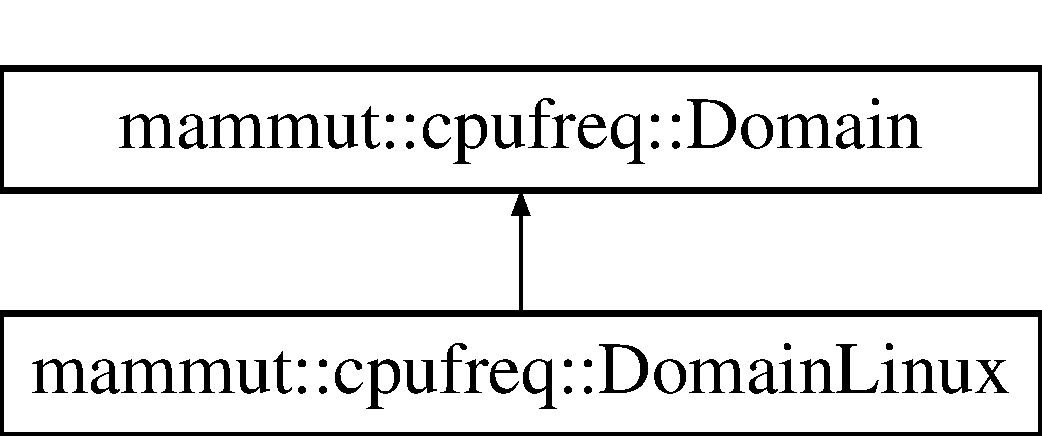
\includegraphics[height=2.000000cm]{classmammut_1_1cpufreq_1_1DomainLinux}
\end{center}
\end{figure}
\subsection*{Public Member Functions}
\begin{DoxyCompactItemize}
\item 
\hyperlink{classmammut_1_1cpufreq_1_1DomainLinux_a0479968ba0436f75ade42d2c63ca34aa}{Domain\-Linux} (Domain\-Id domain\-Identifier, std\-::vector$<$ \hyperlink{classmammut_1_1topology_1_1VirtualCore}{topology\-::\-Virtual\-Core} $\ast$ $>$ virtual\-Cores)
\item 
std\-::vector$<$ Frequency $>$ \hyperlink{classmammut_1_1cpufreq_1_1DomainLinux_a842b3b21fb5fc87c65368dc48cbc02af}{get\-Available\-Frequencies} () const 
\item 
std\-::vector$<$ Governor $>$ \hyperlink{classmammut_1_1cpufreq_1_1DomainLinux_a2596e269900a9567a02cf10b14407bb4}{get\-Available\-Governors} () const 
\item 
Frequency \hyperlink{classmammut_1_1cpufreq_1_1DomainLinux_a31cda10038615a5d98fdf38a67a4682a}{get\-Current\-Frequency} () const 
\item 
Frequency \hyperlink{classmammut_1_1cpufreq_1_1DomainLinux_a22d59973df8f67d8bec1d50e9391cda6}{get\-Current\-Frequency\-Userspace} () const 
\item 
bool \hyperlink{classmammut_1_1cpufreq_1_1DomainLinux_a792ff8e660b86a59703ac0bf9271c53d}{set\-Frequency\-Userspace} (Frequency frequency) const 
\item 
Governor \hyperlink{classmammut_1_1cpufreq_1_1DomainLinux_ab8873a08cc11c89a6119ad87402d130d}{get\-Current\-Governor} () const 
\item 
bool \hyperlink{classmammut_1_1cpufreq_1_1DomainLinux_a3437283a0a9117fb37f68035cc2b6470}{set\-Governor} (Governor governor) const 
\item 
void \hyperlink{classmammut_1_1cpufreq_1_1DomainLinux_a3c92f649d3de3327fdaff788ca7dc8bc}{get\-Hardware\-Frequency\-Bounds} (Frequency \&lower\-Bound, Frequency \&upper\-Bound) const 
\item 
bool \hyperlink{classmammut_1_1cpufreq_1_1DomainLinux_ae84e936d5175b72112ed70a99971d6ae}{get\-Current\-Governor\-Bounds} (Frequency \&lower\-Bound, Frequency \&upper\-Bound) const 
\item 
bool \hyperlink{classmammut_1_1cpufreq_1_1DomainLinux_ab4d990a6ec4d83e23286c0efe28a0c50}{set\-Governor\-Bounds} (Frequency lower\-Bound, Frequency upper\-Bound) const 
\item 
int \hyperlink{classmammut_1_1cpufreq_1_1DomainLinux_a7758f61e7f43ac8ffa63945e44218f4a}{get\-Transition\-Latency} () const 
\item 
Voltage \hyperlink{classmammut_1_1cpufreq_1_1DomainLinux_a32ed27f14678d73b904b7810e0cef19c}{get\-Current\-Voltage} () const 
\item 
Voltage\-Table \hyperlink{classmammut_1_1cpufreq_1_1DomainLinux_abe2cc1707083e66686e32f82a06a4b8b}{get\-Voltage\-Table} (bool only\-Physical\-Cores=true) const 
\item 
Voltage\-Table \hyperlink{classmammut_1_1cpufreq_1_1DomainLinux_a851ab4324c9612340a0d33e670a0aa14}{get\-Voltage\-Table} (uint num\-Virtual\-Cores, bool only\-Physical\-Cores) const 
\end{DoxyCompactItemize}
\subsection*{Additional Inherited Members}


\subsection{Constructor \& Destructor Documentation}
\hypertarget{classmammut_1_1cpufreq_1_1DomainLinux_a0479968ba0436f75ade42d2c63ca34aa}{\index{mammut\-::cpufreq\-::\-Domain\-Linux@{mammut\-::cpufreq\-::\-Domain\-Linux}!Domain\-Linux@{Domain\-Linux}}
\index{Domain\-Linux@{Domain\-Linux}!mammut::cpufreq::DomainLinux@{mammut\-::cpufreq\-::\-Domain\-Linux}}
\subsubsection[{Domain\-Linux}]{\setlength{\rightskip}{0pt plus 5cm}mammut\-::cpufreq\-::\-Domain\-Linux\-::\-Domain\-Linux (
\begin{DoxyParamCaption}
\item[{Domain\-Id}]{domain\-Identifier, }
\item[{std\-::vector$<$ {\bf topology\-::\-Virtual\-Core} $\ast$ $>$}]{virtual\-Cores}
\end{DoxyParamCaption}
)}}\label{classmammut_1_1cpufreq_1_1DomainLinux_a0479968ba0436f75ade42d2c63ca34aa}
Reads available frequecies.

Remove turbo frequency if present.

Reads available governors. 

\subsection{Member Function Documentation}
\hypertarget{classmammut_1_1cpufreq_1_1DomainLinux_a842b3b21fb5fc87c65368dc48cbc02af}{\index{mammut\-::cpufreq\-::\-Domain\-Linux@{mammut\-::cpufreq\-::\-Domain\-Linux}!get\-Available\-Frequencies@{get\-Available\-Frequencies}}
\index{get\-Available\-Frequencies@{get\-Available\-Frequencies}!mammut::cpufreq::DomainLinux@{mammut\-::cpufreq\-::\-Domain\-Linux}}
\subsubsection[{get\-Available\-Frequencies}]{\setlength{\rightskip}{0pt plus 5cm}vector$<$ Frequency $>$ mammut\-::cpufreq\-::\-Domain\-Linux\-::get\-Available\-Frequencies (
\begin{DoxyParamCaption}
{}
\end{DoxyParamCaption}
) const\hspace{0.3cm}{\ttfamily [virtual]}}}\label{classmammut_1_1cpufreq_1_1DomainLinux_a842b3b21fb5fc87c65368dc48cbc02af}
Gets the frequency steps (in K\-Hz) available (sorted from lowest to highest). \begin{DoxyReturn}{Returns}
The frequency steps (in K\-Hz) available (sorted from lowest to highest). 
\end{DoxyReturn}


Implements \hyperlink{classmammut_1_1cpufreq_1_1Domain_a77f57f47e688a3aaae168a2f9e8dc062}{mammut\-::cpufreq\-::\-Domain}.

\hypertarget{classmammut_1_1cpufreq_1_1DomainLinux_a2596e269900a9567a02cf10b14407bb4}{\index{mammut\-::cpufreq\-::\-Domain\-Linux@{mammut\-::cpufreq\-::\-Domain\-Linux}!get\-Available\-Governors@{get\-Available\-Governors}}
\index{get\-Available\-Governors@{get\-Available\-Governors}!mammut::cpufreq::DomainLinux@{mammut\-::cpufreq\-::\-Domain\-Linux}}
\subsubsection[{get\-Available\-Governors}]{\setlength{\rightskip}{0pt plus 5cm}vector$<$ Governor $>$ mammut\-::cpufreq\-::\-Domain\-Linux\-::get\-Available\-Governors (
\begin{DoxyParamCaption}
{}
\end{DoxyParamCaption}
) const\hspace{0.3cm}{\ttfamily [virtual]}}}\label{classmammut_1_1cpufreq_1_1DomainLinux_a2596e269900a9567a02cf10b14407bb4}
Gets the governors available. \begin{DoxyReturn}{Returns}
The governors available. 
\end{DoxyReturn}


Implements \hyperlink{classmammut_1_1cpufreq_1_1Domain_ab72f441a05214166a07c4ece122f02c6}{mammut\-::cpufreq\-::\-Domain}.

\hypertarget{classmammut_1_1cpufreq_1_1DomainLinux_a31cda10038615a5d98fdf38a67a4682a}{\index{mammut\-::cpufreq\-::\-Domain\-Linux@{mammut\-::cpufreq\-::\-Domain\-Linux}!get\-Current\-Frequency@{get\-Current\-Frequency}}
\index{get\-Current\-Frequency@{get\-Current\-Frequency}!mammut::cpufreq::DomainLinux@{mammut\-::cpufreq\-::\-Domain\-Linux}}
\subsubsection[{get\-Current\-Frequency}]{\setlength{\rightskip}{0pt plus 5cm}Frequency mammut\-::cpufreq\-::\-Domain\-Linux\-::get\-Current\-Frequency (
\begin{DoxyParamCaption}
{}
\end{DoxyParamCaption}
) const\hspace{0.3cm}{\ttfamily [virtual]}}}\label{classmammut_1_1cpufreq_1_1DomainLinux_a31cda10038615a5d98fdf38a67a4682a}
Gets the current frequency. \begin{DoxyReturn}{Returns}
The current frequency. 
\end{DoxyReturn}


Implements \hyperlink{classmammut_1_1cpufreq_1_1Domain_a915d7a5e4da2fe377c9805e86820ac3e}{mammut\-::cpufreq\-::\-Domain}.

\hypertarget{classmammut_1_1cpufreq_1_1DomainLinux_a22d59973df8f67d8bec1d50e9391cda6}{\index{mammut\-::cpufreq\-::\-Domain\-Linux@{mammut\-::cpufreq\-::\-Domain\-Linux}!get\-Current\-Frequency\-Userspace@{get\-Current\-Frequency\-Userspace}}
\index{get\-Current\-Frequency\-Userspace@{get\-Current\-Frequency\-Userspace}!mammut::cpufreq::DomainLinux@{mammut\-::cpufreq\-::\-Domain\-Linux}}
\subsubsection[{get\-Current\-Frequency\-Userspace}]{\setlength{\rightskip}{0pt plus 5cm}Frequency mammut\-::cpufreq\-::\-Domain\-Linux\-::get\-Current\-Frequency\-Userspace (
\begin{DoxyParamCaption}
{}
\end{DoxyParamCaption}
) const\hspace{0.3cm}{\ttfamily [virtual]}}}\label{classmammut_1_1cpufreq_1_1DomainLinux_a22d59973df8f67d8bec1d50e9391cda6}
Gets the current frequency set by userspace governor. \begin{DoxyReturn}{Returns}
The current frequency if the current governor is userspace, a meaningless value otherwise. 
\end{DoxyReturn}


Implements \hyperlink{classmammut_1_1cpufreq_1_1Domain_abb5e1908d54a2af862e78b03a1a85af4}{mammut\-::cpufreq\-::\-Domain}.

\hypertarget{classmammut_1_1cpufreq_1_1DomainLinux_ab8873a08cc11c89a6119ad87402d130d}{\index{mammut\-::cpufreq\-::\-Domain\-Linux@{mammut\-::cpufreq\-::\-Domain\-Linux}!get\-Current\-Governor@{get\-Current\-Governor}}
\index{get\-Current\-Governor@{get\-Current\-Governor}!mammut::cpufreq::DomainLinux@{mammut\-::cpufreq\-::\-Domain\-Linux}}
\subsubsection[{get\-Current\-Governor}]{\setlength{\rightskip}{0pt plus 5cm}Governor mammut\-::cpufreq\-::\-Domain\-Linux\-::get\-Current\-Governor (
\begin{DoxyParamCaption}
{}
\end{DoxyParamCaption}
) const\hspace{0.3cm}{\ttfamily [virtual]}}}\label{classmammut_1_1cpufreq_1_1DomainLinux_ab8873a08cc11c89a6119ad87402d130d}
Gets the current governor. \begin{DoxyReturn}{Returns}
The current governor. 
\end{DoxyReturn}


Implements \hyperlink{classmammut_1_1cpufreq_1_1Domain_a938483ec97ed59d0559758a1a467dc62}{mammut\-::cpufreq\-::\-Domain}.

\hypertarget{classmammut_1_1cpufreq_1_1DomainLinux_ae84e936d5175b72112ed70a99971d6ae}{\index{mammut\-::cpufreq\-::\-Domain\-Linux@{mammut\-::cpufreq\-::\-Domain\-Linux}!get\-Current\-Governor\-Bounds@{get\-Current\-Governor\-Bounds}}
\index{get\-Current\-Governor\-Bounds@{get\-Current\-Governor\-Bounds}!mammut::cpufreq::DomainLinux@{mammut\-::cpufreq\-::\-Domain\-Linux}}
\subsubsection[{get\-Current\-Governor\-Bounds}]{\setlength{\rightskip}{0pt plus 5cm}bool mammut\-::cpufreq\-::\-Domain\-Linux\-::get\-Current\-Governor\-Bounds (
\begin{DoxyParamCaption}
\item[{Frequency \&}]{lower\-Bound, }
\item[{Frequency \&}]{upper\-Bound}
\end{DoxyParamCaption}
) const\hspace{0.3cm}{\ttfamily [virtual]}}}\label{classmammut_1_1cpufreq_1_1DomainLinux_ae84e936d5175b72112ed70a99971d6ae}
Gets the current frequency bounds for the governor. 
\begin{DoxyParams}{Parameters}
{\em lower\-Bound} & The current frequency lower bound (specified in k\-H\-Z). \\
\hline
{\em upper\-Bound} & The current frequency upper bound (specified in k\-H\-Z). \\
\hline
\end{DoxyParams}
\begin{DoxyReturn}{Returns}
true if the governor is not userspace, false otherwise. 
\end{DoxyReturn}


Implements \hyperlink{classmammut_1_1cpufreq_1_1Domain_af95ae412f43dfbf60a77715ef4684c0f}{mammut\-::cpufreq\-::\-Domain}.

\hypertarget{classmammut_1_1cpufreq_1_1DomainLinux_a32ed27f14678d73b904b7810e0cef19c}{\index{mammut\-::cpufreq\-::\-Domain\-Linux@{mammut\-::cpufreq\-::\-Domain\-Linux}!get\-Current\-Voltage@{get\-Current\-Voltage}}
\index{get\-Current\-Voltage@{get\-Current\-Voltage}!mammut::cpufreq::DomainLinux@{mammut\-::cpufreq\-::\-Domain\-Linux}}
\subsubsection[{get\-Current\-Voltage}]{\setlength{\rightskip}{0pt plus 5cm}Voltage mammut\-::cpufreq\-::\-Domain\-Linux\-::get\-Current\-Voltage (
\begin{DoxyParamCaption}
{}
\end{DoxyParamCaption}
) const\hspace{0.3cm}{\ttfamily [virtual]}}}\label{classmammut_1_1cpufreq_1_1DomainLinux_a32ed27f14678d73b904b7810e0cef19c}
Returns the current voltage of this domain. \begin{DoxyReturn}{Returns}
The current voltage of this domain. It returns 0 if is not possible to read the current voltage on this domain. 
\end{DoxyReturn}


Implements \hyperlink{classmammut_1_1cpufreq_1_1Domain_acd823bdc2f011c042dbb272c4d63df3c}{mammut\-::cpufreq\-::\-Domain}.

\hypertarget{classmammut_1_1cpufreq_1_1DomainLinux_a3c92f649d3de3327fdaff788ca7dc8bc}{\index{mammut\-::cpufreq\-::\-Domain\-Linux@{mammut\-::cpufreq\-::\-Domain\-Linux}!get\-Hardware\-Frequency\-Bounds@{get\-Hardware\-Frequency\-Bounds}}
\index{get\-Hardware\-Frequency\-Bounds@{get\-Hardware\-Frequency\-Bounds}!mammut::cpufreq::DomainLinux@{mammut\-::cpufreq\-::\-Domain\-Linux}}
\subsubsection[{get\-Hardware\-Frequency\-Bounds}]{\setlength{\rightskip}{0pt plus 5cm}void mammut\-::cpufreq\-::\-Domain\-Linux\-::get\-Hardware\-Frequency\-Bounds (
\begin{DoxyParamCaption}
\item[{Frequency \&}]{lower\-Bound, }
\item[{Frequency \&}]{upper\-Bound}
\end{DoxyParamCaption}
) const\hspace{0.3cm}{\ttfamily [virtual]}}}\label{classmammut_1_1cpufreq_1_1DomainLinux_a3c92f649d3de3327fdaff788ca7dc8bc}
Gets the hardware frequency bounds. 
\begin{DoxyParams}{Parameters}
{\em lower\-Bound} & The hardware frequency lower bound (specified in k\-H\-Z). \\
\hline
{\em upper\-Bound} & The hardware frequency upper bound (specified in k\-H\-Z). \\
\hline
\end{DoxyParams}


Implements \hyperlink{classmammut_1_1cpufreq_1_1Domain_a652712c9192a755fb2bc6b58076eccb8}{mammut\-::cpufreq\-::\-Domain}.

\hypertarget{classmammut_1_1cpufreq_1_1DomainLinux_a7758f61e7f43ac8ffa63945e44218f4a}{\index{mammut\-::cpufreq\-::\-Domain\-Linux@{mammut\-::cpufreq\-::\-Domain\-Linux}!get\-Transition\-Latency@{get\-Transition\-Latency}}
\index{get\-Transition\-Latency@{get\-Transition\-Latency}!mammut::cpufreq::DomainLinux@{mammut\-::cpufreq\-::\-Domain\-Linux}}
\subsubsection[{get\-Transition\-Latency}]{\setlength{\rightskip}{0pt plus 5cm}int mammut\-::cpufreq\-::\-Domain\-Linux\-::get\-Transition\-Latency (
\begin{DoxyParamCaption}
{}
\end{DoxyParamCaption}
) const\hspace{0.3cm}{\ttfamily [virtual]}}}\label{classmammut_1_1cpufreq_1_1DomainLinux_a7758f61e7f43ac8ffa63945e44218f4a}
Returns the frequency transition latency (nanoseconds). \begin{DoxyReturn}{Returns}
The frequency transition latency (nanoseconds). -\/1 will be returned if the latency is unknown. 
\end{DoxyReturn}


Implements \hyperlink{classmammut_1_1cpufreq_1_1Domain_a0c7d34dc9ee1e5eb57200a127ae9f183}{mammut\-::cpufreq\-::\-Domain}.

\hypertarget{classmammut_1_1cpufreq_1_1DomainLinux_abe2cc1707083e66686e32f82a06a4b8b}{\index{mammut\-::cpufreq\-::\-Domain\-Linux@{mammut\-::cpufreq\-::\-Domain\-Linux}!get\-Voltage\-Table@{get\-Voltage\-Table}}
\index{get\-Voltage\-Table@{get\-Voltage\-Table}!mammut::cpufreq::DomainLinux@{mammut\-::cpufreq\-::\-Domain\-Linux}}
\subsubsection[{get\-Voltage\-Table}]{\setlength{\rightskip}{0pt plus 5cm}Voltage\-Table mammut\-::cpufreq\-::\-Domain\-Linux\-::get\-Voltage\-Table (
\begin{DoxyParamCaption}
\item[{bool}]{only\-Physical\-Cores = {\ttfamily true}}
\end{DoxyParamCaption}
) const\hspace{0.3cm}{\ttfamily [virtual]}}}\label{classmammut_1_1cpufreq_1_1DomainLinux_abe2cc1707083e66686e32f82a06a4b8b}
Returns the voltage table of this domain. The voltage table is a map where for each pair $<$N, F$>$ is associated a voltage V. N is the number of virtual cores running at frequency F at 100\% of load. N\-O\-T\-E\-: This call may block the caller for some seconds/minutes. 
\begin{DoxyParams}{Parameters}
{\em only\-Physical\-Cores} & If true, only physical cores will be considered. \\
\hline
\end{DoxyParams}
\begin{DoxyReturn}{Returns}
The voltage table of this domain. If voltages cannot be read, the table will be empty. 
\end{DoxyReturn}


Implements \hyperlink{classmammut_1_1cpufreq_1_1Domain_ad0b11fad2e36e45d6028de662df63ba8}{mammut\-::cpufreq\-::\-Domain}.

\hypertarget{classmammut_1_1cpufreq_1_1DomainLinux_a851ab4324c9612340a0d33e670a0aa14}{\index{mammut\-::cpufreq\-::\-Domain\-Linux@{mammut\-::cpufreq\-::\-Domain\-Linux}!get\-Voltage\-Table@{get\-Voltage\-Table}}
\index{get\-Voltage\-Table@{get\-Voltage\-Table}!mammut::cpufreq::DomainLinux@{mammut\-::cpufreq\-::\-Domain\-Linux}}
\subsubsection[{get\-Voltage\-Table}]{\setlength{\rightskip}{0pt plus 5cm}Voltage\-Table mammut\-::cpufreq\-::\-Domain\-Linux\-::get\-Voltage\-Table (
\begin{DoxyParamCaption}
\item[{uint}]{num\-Virtual\-Cores, }
\item[{bool}]{only\-Physical\-Cores}
\end{DoxyParamCaption}
) const\hspace{0.3cm}{\ttfamily [virtual]}}}\label{classmammut_1_1cpufreq_1_1DomainLinux_a851ab4324c9612340a0d33e670a0aa14}
Returns the voltage table of this domain. For a specific number of virtual cores N. The voltage table is a map where for each pair $<$N, F$>$ is associated a voltage V. N is the number of virtual cores running at frequency F at 100\% of load. N\-O\-T\-E\-: This call may block the caller for some seconds/minutes. 
\begin{DoxyParams}{Parameters}
{\em num\-Virtual\-Cores} & The number of virtual cores. \\
\hline
{\em only\-Physical\-Cores} & If true, only physical cores will be considered. \\
\hline
\end{DoxyParams}
\begin{DoxyReturn}{Returns}
The voltage table of this domain. If voltages cannot be read, the table will be empty. 
\end{DoxyReturn}


Implements \hyperlink{classmammut_1_1cpufreq_1_1Domain_a4442dfd2b7d52a95ad4bdf3e99185bf3}{mammut\-::cpufreq\-::\-Domain}.

\hypertarget{classmammut_1_1cpufreq_1_1DomainLinux_a792ff8e660b86a59703ac0bf9271c53d}{\index{mammut\-::cpufreq\-::\-Domain\-Linux@{mammut\-::cpufreq\-::\-Domain\-Linux}!set\-Frequency\-Userspace@{set\-Frequency\-Userspace}}
\index{set\-Frequency\-Userspace@{set\-Frequency\-Userspace}!mammut::cpufreq::DomainLinux@{mammut\-::cpufreq\-::\-Domain\-Linux}}
\subsubsection[{set\-Frequency\-Userspace}]{\setlength{\rightskip}{0pt plus 5cm}bool mammut\-::cpufreq\-::\-Domain\-Linux\-::set\-Frequency\-Userspace (
\begin{DoxyParamCaption}
\item[{Frequency}]{frequency}
\end{DoxyParamCaption}
) const\hspace{0.3cm}{\ttfamily [virtual]}}}\label{classmammut_1_1cpufreq_1_1DomainLinux_a792ff8e660b86a59703ac0bf9271c53d}
Change the running frequency. 
\begin{DoxyParams}{Parameters}
{\em frequency} & The frequency to be set (specified in k\-H\-Z). \\
\hline
\end{DoxyParams}
\begin{DoxyReturn}{Returns}
true if the frequency is valid and the governor is userspace, false otherwise. 
\end{DoxyReturn}


Implements \hyperlink{classmammut_1_1cpufreq_1_1Domain_a6f97e04fa138bbb6b478c8a7338b4116}{mammut\-::cpufreq\-::\-Domain}.

\hypertarget{classmammut_1_1cpufreq_1_1DomainLinux_a3437283a0a9117fb37f68035cc2b6470}{\index{mammut\-::cpufreq\-::\-Domain\-Linux@{mammut\-::cpufreq\-::\-Domain\-Linux}!set\-Governor@{set\-Governor}}
\index{set\-Governor@{set\-Governor}!mammut::cpufreq::DomainLinux@{mammut\-::cpufreq\-::\-Domain\-Linux}}
\subsubsection[{set\-Governor}]{\setlength{\rightskip}{0pt plus 5cm}bool mammut\-::cpufreq\-::\-Domain\-Linux\-::set\-Governor (
\begin{DoxyParamCaption}
\item[{Governor}]{governor}
\end{DoxyParamCaption}
) const\hspace{0.3cm}{\ttfamily [virtual]}}}\label{classmammut_1_1cpufreq_1_1DomainLinux_a3437283a0a9117fb37f68035cc2b6470}
Changes the governor. 
\begin{DoxyParams}{Parameters}
{\em governor} & The identifier of the governor. \\
\hline
\end{DoxyParams}
\begin{DoxyReturn}{Returns}
true if the governor is valid, false otherwise. 
\end{DoxyReturn}


Implements \hyperlink{classmammut_1_1cpufreq_1_1Domain_a48cb064376b9b663e5a134a61b5780bd}{mammut\-::cpufreq\-::\-Domain}.

\hypertarget{classmammut_1_1cpufreq_1_1DomainLinux_ab4d990a6ec4d83e23286c0efe28a0c50}{\index{mammut\-::cpufreq\-::\-Domain\-Linux@{mammut\-::cpufreq\-::\-Domain\-Linux}!set\-Governor\-Bounds@{set\-Governor\-Bounds}}
\index{set\-Governor\-Bounds@{set\-Governor\-Bounds}!mammut::cpufreq::DomainLinux@{mammut\-::cpufreq\-::\-Domain\-Linux}}
\subsubsection[{set\-Governor\-Bounds}]{\setlength{\rightskip}{0pt plus 5cm}bool mammut\-::cpufreq\-::\-Domain\-Linux\-::set\-Governor\-Bounds (
\begin{DoxyParamCaption}
\item[{Frequency}]{lower\-Bound, }
\item[{Frequency}]{upper\-Bound}
\end{DoxyParamCaption}
) const\hspace{0.3cm}{\ttfamily [virtual]}}}\label{classmammut_1_1cpufreq_1_1DomainLinux_ab4d990a6ec4d83e23286c0efe28a0c50}
Change the frequency bounds of the governor. 
\begin{DoxyParams}{Parameters}
{\em lower\-Bound} & The new frequency lower bound (specified in k\-H\-Z). \\
\hline
{\em upper\-Bound} & The new frequency upper bound (specified in k\-H\-Z). \\
\hline
\end{DoxyParams}
\begin{DoxyReturn}{Returns}
true if the bounds are valid and the governor is not userspace, false otherwise. 
\end{DoxyReturn}


Implements \hyperlink{classmammut_1_1cpufreq_1_1Domain_a45a0a69b4957937c921e723bbcf6cf04}{mammut\-::cpufreq\-::\-Domain}.



The documentation for this class was generated from the following files\-:\begin{DoxyCompactItemize}
\item 
/home/daniele/\-Code/\-Mammut/mammut/cpufreq/cpufreq-\/linux.\-hpp\item 
/home/daniele/\-Code/\-Mammut/mammut/cpufreq/cpufreq-\/linux.\-cpp\end{DoxyCompactItemize}

\hypertarget{classmammut_1_1cpufreq_1_1DomainRemote}{\section{mammut\-:\-:cpufreq\-:\-:Domain\-Remote Class Reference}
\label{classmammut_1_1cpufreq_1_1DomainRemote}\index{mammut\-::cpufreq\-::\-Domain\-Remote@{mammut\-::cpufreq\-::\-Domain\-Remote}}
}
Inheritance diagram for mammut\-:\-:cpufreq\-:\-:Domain\-Remote\-:\begin{figure}[H]
\begin{center}
\leavevmode
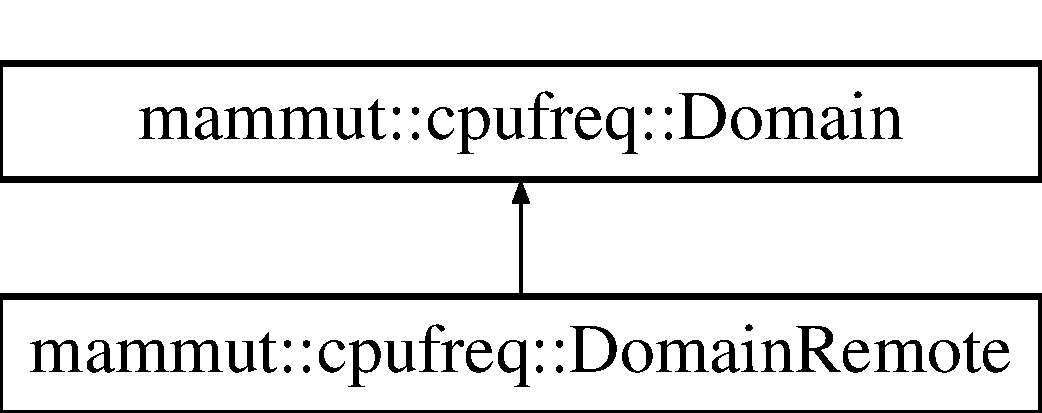
\includegraphics[height=2.000000cm]{classmammut_1_1cpufreq_1_1DomainRemote}
\end{center}
\end{figure}
\subsection*{Public Member Functions}
\begin{DoxyCompactItemize}
\item 
\hypertarget{classmammut_1_1cpufreq_1_1DomainRemote_a29f8a1cf54c6457a7b0fb5b01fbec790}{{\bfseries Domain\-Remote} (\hyperlink{classmammut_1_1Communicator}{Communicator} $\ast$const communicator, Domain\-Id domain\-Identifier, std\-::vector$<$ \hyperlink{classmammut_1_1topology_1_1VirtualCore}{topology\-::\-Virtual\-Core} $\ast$ $>$ virtual\-Cores)}\label{classmammut_1_1cpufreq_1_1DomainRemote_a29f8a1cf54c6457a7b0fb5b01fbec790}

\item 
std\-::vector$<$ Frequency $>$ \hyperlink{classmammut_1_1cpufreq_1_1DomainRemote_a07132aa88d0c49d2f48a01e47604ae39}{get\-Available\-Frequencies} () const 
\item 
std\-::vector$<$ Governor $>$ \hyperlink{classmammut_1_1cpufreq_1_1DomainRemote_a125ba0d251841a14853fb9830564fba8}{get\-Available\-Governors} () const 
\item 
Frequency \hyperlink{classmammut_1_1cpufreq_1_1DomainRemote_a080d7be95c68f1dc57510a1fe4765f65}{get\-Current\-Frequency} () const 
\item 
Frequency \hyperlink{classmammut_1_1cpufreq_1_1DomainRemote_a0202e17b3b2a9ff30b711c5157ec9a86}{get\-Current\-Frequency\-Userspace} () const 
\item 
bool \hyperlink{classmammut_1_1cpufreq_1_1DomainRemote_ad35211bbe0ed2e8bb0f31e0942ec21d2}{set\-Frequency\-Userspace} (Frequency frequency) const 
\item 
Governor \hyperlink{classmammut_1_1cpufreq_1_1DomainRemote_a44628a8aa9d605e683c3273ddbe549b7}{get\-Current\-Governor} () const 
\item 
bool \hyperlink{classmammut_1_1cpufreq_1_1DomainRemote_ab8d851c0880768b373130bdaca889e50}{set\-Governor} (Governor governor) const 
\item 
void \hyperlink{classmammut_1_1cpufreq_1_1DomainRemote_a2343f9e0b325f549062a3df160945ae5}{get\-Hardware\-Frequency\-Bounds} (Frequency \&lower\-Bound, Frequency \&upper\-Bound) const 
\item 
bool \hyperlink{classmammut_1_1cpufreq_1_1DomainRemote_a351e9fc310205750a81417b5d5e278e0}{get\-Current\-Governor\-Bounds} (Frequency \&lower\-Bound, Frequency \&upper\-Bound) const 
\item 
bool \hyperlink{classmammut_1_1cpufreq_1_1DomainRemote_a4e2fc1bc7556ebebda702fb13a9d2418}{set\-Governor\-Bounds} (Frequency lower\-Bound, Frequency upper\-Bound) const 
\item 
int \hyperlink{classmammut_1_1cpufreq_1_1DomainRemote_a9f7670fb58123145482a0e0ae7afb5cf}{get\-Transition\-Latency} () const 
\item 
Voltage \hyperlink{classmammut_1_1cpufreq_1_1DomainRemote_ad1277e302f2c1e649be0d0ef5b55f6f3}{get\-Current\-Voltage} () const 
\item 
Voltage\-Table \hyperlink{classmammut_1_1cpufreq_1_1DomainRemote_af8b22d85101c9c19ce1f2afaf287e474}{get\-Voltage\-Table} (bool only\-Physical\-Cores) const 
\item 
Voltage\-Table \hyperlink{classmammut_1_1cpufreq_1_1DomainRemote_a00226c85ab71dac250755e100776b55c}{get\-Voltage\-Table} (uint num\-Virtual\-Cores, bool only\-Physical\-Cores) const 
\end{DoxyCompactItemize}
\subsection*{Additional Inherited Members}


\subsection{Member Function Documentation}
\hypertarget{classmammut_1_1cpufreq_1_1DomainRemote_a07132aa88d0c49d2f48a01e47604ae39}{\index{mammut\-::cpufreq\-::\-Domain\-Remote@{mammut\-::cpufreq\-::\-Domain\-Remote}!get\-Available\-Frequencies@{get\-Available\-Frequencies}}
\index{get\-Available\-Frequencies@{get\-Available\-Frequencies}!mammut::cpufreq::DomainRemote@{mammut\-::cpufreq\-::\-Domain\-Remote}}
\subsubsection[{get\-Available\-Frequencies}]{\setlength{\rightskip}{0pt plus 5cm}std\-::vector$<$Frequency$>$ mammut\-::cpufreq\-::\-Domain\-Remote\-::get\-Available\-Frequencies (
\begin{DoxyParamCaption}
{}
\end{DoxyParamCaption}
) const\hspace{0.3cm}{\ttfamily [virtual]}}}\label{classmammut_1_1cpufreq_1_1DomainRemote_a07132aa88d0c49d2f48a01e47604ae39}
Gets the frequency steps (in K\-Hz) available (sorted from lowest to highest). \begin{DoxyReturn}{Returns}
The frequency steps (in K\-Hz) available (sorted from lowest to highest). 
\end{DoxyReturn}


Implements \hyperlink{classmammut_1_1cpufreq_1_1Domain_a77f57f47e688a3aaae168a2f9e8dc062}{mammut\-::cpufreq\-::\-Domain}.

\hypertarget{classmammut_1_1cpufreq_1_1DomainRemote_a125ba0d251841a14853fb9830564fba8}{\index{mammut\-::cpufreq\-::\-Domain\-Remote@{mammut\-::cpufreq\-::\-Domain\-Remote}!get\-Available\-Governors@{get\-Available\-Governors}}
\index{get\-Available\-Governors@{get\-Available\-Governors}!mammut::cpufreq::DomainRemote@{mammut\-::cpufreq\-::\-Domain\-Remote}}
\subsubsection[{get\-Available\-Governors}]{\setlength{\rightskip}{0pt plus 5cm}std\-::vector$<$Governor$>$ mammut\-::cpufreq\-::\-Domain\-Remote\-::get\-Available\-Governors (
\begin{DoxyParamCaption}
{}
\end{DoxyParamCaption}
) const\hspace{0.3cm}{\ttfamily [virtual]}}}\label{classmammut_1_1cpufreq_1_1DomainRemote_a125ba0d251841a14853fb9830564fba8}
Gets the governors available. \begin{DoxyReturn}{Returns}
The governors available. 
\end{DoxyReturn}


Implements \hyperlink{classmammut_1_1cpufreq_1_1Domain_ab72f441a05214166a07c4ece122f02c6}{mammut\-::cpufreq\-::\-Domain}.

\hypertarget{classmammut_1_1cpufreq_1_1DomainRemote_a080d7be95c68f1dc57510a1fe4765f65}{\index{mammut\-::cpufreq\-::\-Domain\-Remote@{mammut\-::cpufreq\-::\-Domain\-Remote}!get\-Current\-Frequency@{get\-Current\-Frequency}}
\index{get\-Current\-Frequency@{get\-Current\-Frequency}!mammut::cpufreq::DomainRemote@{mammut\-::cpufreq\-::\-Domain\-Remote}}
\subsubsection[{get\-Current\-Frequency}]{\setlength{\rightskip}{0pt plus 5cm}Frequency mammut\-::cpufreq\-::\-Domain\-Remote\-::get\-Current\-Frequency (
\begin{DoxyParamCaption}
{}
\end{DoxyParamCaption}
) const\hspace{0.3cm}{\ttfamily [virtual]}}}\label{classmammut_1_1cpufreq_1_1DomainRemote_a080d7be95c68f1dc57510a1fe4765f65}
Gets the current frequency. \begin{DoxyReturn}{Returns}
The current frequency. 
\end{DoxyReturn}


Implements \hyperlink{classmammut_1_1cpufreq_1_1Domain_a915d7a5e4da2fe377c9805e86820ac3e}{mammut\-::cpufreq\-::\-Domain}.

\hypertarget{classmammut_1_1cpufreq_1_1DomainRemote_a0202e17b3b2a9ff30b711c5157ec9a86}{\index{mammut\-::cpufreq\-::\-Domain\-Remote@{mammut\-::cpufreq\-::\-Domain\-Remote}!get\-Current\-Frequency\-Userspace@{get\-Current\-Frequency\-Userspace}}
\index{get\-Current\-Frequency\-Userspace@{get\-Current\-Frequency\-Userspace}!mammut::cpufreq::DomainRemote@{mammut\-::cpufreq\-::\-Domain\-Remote}}
\subsubsection[{get\-Current\-Frequency\-Userspace}]{\setlength{\rightskip}{0pt plus 5cm}Frequency mammut\-::cpufreq\-::\-Domain\-Remote\-::get\-Current\-Frequency\-Userspace (
\begin{DoxyParamCaption}
{}
\end{DoxyParamCaption}
) const\hspace{0.3cm}{\ttfamily [virtual]}}}\label{classmammut_1_1cpufreq_1_1DomainRemote_a0202e17b3b2a9ff30b711c5157ec9a86}
Gets the current frequency set by userspace governor. \begin{DoxyReturn}{Returns}
The current frequency if the current governor is userspace, a meaningless value otherwise. 
\end{DoxyReturn}


Implements \hyperlink{classmammut_1_1cpufreq_1_1Domain_abb5e1908d54a2af862e78b03a1a85af4}{mammut\-::cpufreq\-::\-Domain}.

\hypertarget{classmammut_1_1cpufreq_1_1DomainRemote_a44628a8aa9d605e683c3273ddbe549b7}{\index{mammut\-::cpufreq\-::\-Domain\-Remote@{mammut\-::cpufreq\-::\-Domain\-Remote}!get\-Current\-Governor@{get\-Current\-Governor}}
\index{get\-Current\-Governor@{get\-Current\-Governor}!mammut::cpufreq::DomainRemote@{mammut\-::cpufreq\-::\-Domain\-Remote}}
\subsubsection[{get\-Current\-Governor}]{\setlength{\rightskip}{0pt plus 5cm}Governor mammut\-::cpufreq\-::\-Domain\-Remote\-::get\-Current\-Governor (
\begin{DoxyParamCaption}
{}
\end{DoxyParamCaption}
) const\hspace{0.3cm}{\ttfamily [virtual]}}}\label{classmammut_1_1cpufreq_1_1DomainRemote_a44628a8aa9d605e683c3273ddbe549b7}
Gets the current governor. \begin{DoxyReturn}{Returns}
The current governor. 
\end{DoxyReturn}


Implements \hyperlink{classmammut_1_1cpufreq_1_1Domain_a938483ec97ed59d0559758a1a467dc62}{mammut\-::cpufreq\-::\-Domain}.

\hypertarget{classmammut_1_1cpufreq_1_1DomainRemote_a351e9fc310205750a81417b5d5e278e0}{\index{mammut\-::cpufreq\-::\-Domain\-Remote@{mammut\-::cpufreq\-::\-Domain\-Remote}!get\-Current\-Governor\-Bounds@{get\-Current\-Governor\-Bounds}}
\index{get\-Current\-Governor\-Bounds@{get\-Current\-Governor\-Bounds}!mammut::cpufreq::DomainRemote@{mammut\-::cpufreq\-::\-Domain\-Remote}}
\subsubsection[{get\-Current\-Governor\-Bounds}]{\setlength{\rightskip}{0pt plus 5cm}bool mammut\-::cpufreq\-::\-Domain\-Remote\-::get\-Current\-Governor\-Bounds (
\begin{DoxyParamCaption}
\item[{Frequency \&}]{lower\-Bound, }
\item[{Frequency \&}]{upper\-Bound}
\end{DoxyParamCaption}
) const\hspace{0.3cm}{\ttfamily [virtual]}}}\label{classmammut_1_1cpufreq_1_1DomainRemote_a351e9fc310205750a81417b5d5e278e0}
Gets the current frequency bounds for the governor. 
\begin{DoxyParams}{Parameters}
{\em lower\-Bound} & The current frequency lower bound (specified in k\-H\-Z). \\
\hline
{\em upper\-Bound} & The current frequency upper bound (specified in k\-H\-Z). \\
\hline
\end{DoxyParams}
\begin{DoxyReturn}{Returns}
true if the governor is not userspace, false otherwise. 
\end{DoxyReturn}


Implements \hyperlink{classmammut_1_1cpufreq_1_1Domain_af95ae412f43dfbf60a77715ef4684c0f}{mammut\-::cpufreq\-::\-Domain}.

\hypertarget{classmammut_1_1cpufreq_1_1DomainRemote_ad1277e302f2c1e649be0d0ef5b55f6f3}{\index{mammut\-::cpufreq\-::\-Domain\-Remote@{mammut\-::cpufreq\-::\-Domain\-Remote}!get\-Current\-Voltage@{get\-Current\-Voltage}}
\index{get\-Current\-Voltage@{get\-Current\-Voltage}!mammut::cpufreq::DomainRemote@{mammut\-::cpufreq\-::\-Domain\-Remote}}
\subsubsection[{get\-Current\-Voltage}]{\setlength{\rightskip}{0pt plus 5cm}Voltage mammut\-::cpufreq\-::\-Domain\-Remote\-::get\-Current\-Voltage (
\begin{DoxyParamCaption}
{}
\end{DoxyParamCaption}
) const\hspace{0.3cm}{\ttfamily [virtual]}}}\label{classmammut_1_1cpufreq_1_1DomainRemote_ad1277e302f2c1e649be0d0ef5b55f6f3}
Returns the current voltage of this domain. \begin{DoxyReturn}{Returns}
The current voltage of this domain. It returns 0 if is not possible to read the current voltage on this domain. 
\end{DoxyReturn}


Implements \hyperlink{classmammut_1_1cpufreq_1_1Domain_acd823bdc2f011c042dbb272c4d63df3c}{mammut\-::cpufreq\-::\-Domain}.

\hypertarget{classmammut_1_1cpufreq_1_1DomainRemote_a2343f9e0b325f549062a3df160945ae5}{\index{mammut\-::cpufreq\-::\-Domain\-Remote@{mammut\-::cpufreq\-::\-Domain\-Remote}!get\-Hardware\-Frequency\-Bounds@{get\-Hardware\-Frequency\-Bounds}}
\index{get\-Hardware\-Frequency\-Bounds@{get\-Hardware\-Frequency\-Bounds}!mammut::cpufreq::DomainRemote@{mammut\-::cpufreq\-::\-Domain\-Remote}}
\subsubsection[{get\-Hardware\-Frequency\-Bounds}]{\setlength{\rightskip}{0pt plus 5cm}void mammut\-::cpufreq\-::\-Domain\-Remote\-::get\-Hardware\-Frequency\-Bounds (
\begin{DoxyParamCaption}
\item[{Frequency \&}]{lower\-Bound, }
\item[{Frequency \&}]{upper\-Bound}
\end{DoxyParamCaption}
) const\hspace{0.3cm}{\ttfamily [virtual]}}}\label{classmammut_1_1cpufreq_1_1DomainRemote_a2343f9e0b325f549062a3df160945ae5}
Gets the hardware frequency bounds. 
\begin{DoxyParams}{Parameters}
{\em lower\-Bound} & The hardware frequency lower bound (specified in k\-H\-Z). \\
\hline
{\em upper\-Bound} & The hardware frequency upper bound (specified in k\-H\-Z). \\
\hline
\end{DoxyParams}


Implements \hyperlink{classmammut_1_1cpufreq_1_1Domain_a652712c9192a755fb2bc6b58076eccb8}{mammut\-::cpufreq\-::\-Domain}.

\hypertarget{classmammut_1_1cpufreq_1_1DomainRemote_a9f7670fb58123145482a0e0ae7afb5cf}{\index{mammut\-::cpufreq\-::\-Domain\-Remote@{mammut\-::cpufreq\-::\-Domain\-Remote}!get\-Transition\-Latency@{get\-Transition\-Latency}}
\index{get\-Transition\-Latency@{get\-Transition\-Latency}!mammut::cpufreq::DomainRemote@{mammut\-::cpufreq\-::\-Domain\-Remote}}
\subsubsection[{get\-Transition\-Latency}]{\setlength{\rightskip}{0pt plus 5cm}int mammut\-::cpufreq\-::\-Domain\-Remote\-::get\-Transition\-Latency (
\begin{DoxyParamCaption}
{}
\end{DoxyParamCaption}
) const\hspace{0.3cm}{\ttfamily [virtual]}}}\label{classmammut_1_1cpufreq_1_1DomainRemote_a9f7670fb58123145482a0e0ae7afb5cf}
Returns the frequency transition latency (nanoseconds). \begin{DoxyReturn}{Returns}
The frequency transition latency (nanoseconds). -\/1 will be returned if the latency is unknown. 
\end{DoxyReturn}


Implements \hyperlink{classmammut_1_1cpufreq_1_1Domain_a0c7d34dc9ee1e5eb57200a127ae9f183}{mammut\-::cpufreq\-::\-Domain}.

\hypertarget{classmammut_1_1cpufreq_1_1DomainRemote_af8b22d85101c9c19ce1f2afaf287e474}{\index{mammut\-::cpufreq\-::\-Domain\-Remote@{mammut\-::cpufreq\-::\-Domain\-Remote}!get\-Voltage\-Table@{get\-Voltage\-Table}}
\index{get\-Voltage\-Table@{get\-Voltage\-Table}!mammut::cpufreq::DomainRemote@{mammut\-::cpufreq\-::\-Domain\-Remote}}
\subsubsection[{get\-Voltage\-Table}]{\setlength{\rightskip}{0pt plus 5cm}Voltage\-Table mammut\-::cpufreq\-::\-Domain\-Remote\-::get\-Voltage\-Table (
\begin{DoxyParamCaption}
\item[{bool}]{only\-Physical\-Cores}
\end{DoxyParamCaption}
) const\hspace{0.3cm}{\ttfamily [inline]}, {\ttfamily [virtual]}}}\label{classmammut_1_1cpufreq_1_1DomainRemote_af8b22d85101c9c19ce1f2afaf287e474}
Returns the voltage table of this domain. The voltage table is a map where for each pair $<$N, F$>$ is associated a voltage V. N is the number of virtual cores running at frequency F at 100\% of load. N\-O\-T\-E\-: This call may block the caller for some seconds/minutes. 
\begin{DoxyParams}{Parameters}
{\em only\-Physical\-Cores} & If true, only physical cores will be considered. \\
\hline
\end{DoxyParams}
\begin{DoxyReturn}{Returns}
The voltage table of this domain. If voltages cannot be read, the table will be empty. 
\end{DoxyReturn}


Implements \hyperlink{classmammut_1_1cpufreq_1_1Domain_ad0b11fad2e36e45d6028de662df63ba8}{mammut\-::cpufreq\-::\-Domain}.

\hypertarget{classmammut_1_1cpufreq_1_1DomainRemote_a00226c85ab71dac250755e100776b55c}{\index{mammut\-::cpufreq\-::\-Domain\-Remote@{mammut\-::cpufreq\-::\-Domain\-Remote}!get\-Voltage\-Table@{get\-Voltage\-Table}}
\index{get\-Voltage\-Table@{get\-Voltage\-Table}!mammut::cpufreq::DomainRemote@{mammut\-::cpufreq\-::\-Domain\-Remote}}
\subsubsection[{get\-Voltage\-Table}]{\setlength{\rightskip}{0pt plus 5cm}Voltage\-Table mammut\-::cpufreq\-::\-Domain\-Remote\-::get\-Voltage\-Table (
\begin{DoxyParamCaption}
\item[{uint}]{num\-Virtual\-Cores, }
\item[{bool}]{only\-Physical\-Cores}
\end{DoxyParamCaption}
) const\hspace{0.3cm}{\ttfamily [inline]}, {\ttfamily [virtual]}}}\label{classmammut_1_1cpufreq_1_1DomainRemote_a00226c85ab71dac250755e100776b55c}
Returns the voltage table of this domain. For a specific number of virtual cores N. The voltage table is a map where for each pair $<$N, F$>$ is associated a voltage V. N is the number of virtual cores running at frequency F at 100\% of load. N\-O\-T\-E\-: This call may block the caller for some seconds/minutes. 
\begin{DoxyParams}{Parameters}
{\em num\-Virtual\-Cores} & The number of virtual cores. \\
\hline
{\em only\-Physical\-Cores} & If true, only physical cores will be considered. \\
\hline
\end{DoxyParams}
\begin{DoxyReturn}{Returns}
The voltage table of this domain. If voltages cannot be read, the table will be empty. 
\end{DoxyReturn}


Implements \hyperlink{classmammut_1_1cpufreq_1_1Domain_a4442dfd2b7d52a95ad4bdf3e99185bf3}{mammut\-::cpufreq\-::\-Domain}.

\hypertarget{classmammut_1_1cpufreq_1_1DomainRemote_ad35211bbe0ed2e8bb0f31e0942ec21d2}{\index{mammut\-::cpufreq\-::\-Domain\-Remote@{mammut\-::cpufreq\-::\-Domain\-Remote}!set\-Frequency\-Userspace@{set\-Frequency\-Userspace}}
\index{set\-Frequency\-Userspace@{set\-Frequency\-Userspace}!mammut::cpufreq::DomainRemote@{mammut\-::cpufreq\-::\-Domain\-Remote}}
\subsubsection[{set\-Frequency\-Userspace}]{\setlength{\rightskip}{0pt plus 5cm}bool mammut\-::cpufreq\-::\-Domain\-Remote\-::set\-Frequency\-Userspace (
\begin{DoxyParamCaption}
\item[{Frequency}]{frequency}
\end{DoxyParamCaption}
) const\hspace{0.3cm}{\ttfamily [virtual]}}}\label{classmammut_1_1cpufreq_1_1DomainRemote_ad35211bbe0ed2e8bb0f31e0942ec21d2}
Change the running frequency. 
\begin{DoxyParams}{Parameters}
{\em frequency} & The frequency to be set (specified in k\-H\-Z). \\
\hline
\end{DoxyParams}
\begin{DoxyReturn}{Returns}
true if the frequency is valid and the governor is userspace, false otherwise. 
\end{DoxyReturn}


Implements \hyperlink{classmammut_1_1cpufreq_1_1Domain_a6f97e04fa138bbb6b478c8a7338b4116}{mammut\-::cpufreq\-::\-Domain}.

\hypertarget{classmammut_1_1cpufreq_1_1DomainRemote_ab8d851c0880768b373130bdaca889e50}{\index{mammut\-::cpufreq\-::\-Domain\-Remote@{mammut\-::cpufreq\-::\-Domain\-Remote}!set\-Governor@{set\-Governor}}
\index{set\-Governor@{set\-Governor}!mammut::cpufreq::DomainRemote@{mammut\-::cpufreq\-::\-Domain\-Remote}}
\subsubsection[{set\-Governor}]{\setlength{\rightskip}{0pt plus 5cm}bool mammut\-::cpufreq\-::\-Domain\-Remote\-::set\-Governor (
\begin{DoxyParamCaption}
\item[{Governor}]{governor}
\end{DoxyParamCaption}
) const\hspace{0.3cm}{\ttfamily [virtual]}}}\label{classmammut_1_1cpufreq_1_1DomainRemote_ab8d851c0880768b373130bdaca889e50}
Changes the governor. 
\begin{DoxyParams}{Parameters}
{\em governor} & The identifier of the governor. \\
\hline
\end{DoxyParams}
\begin{DoxyReturn}{Returns}
true if the governor is valid, false otherwise. 
\end{DoxyReturn}


Implements \hyperlink{classmammut_1_1cpufreq_1_1Domain_a48cb064376b9b663e5a134a61b5780bd}{mammut\-::cpufreq\-::\-Domain}.

\hypertarget{classmammut_1_1cpufreq_1_1DomainRemote_a4e2fc1bc7556ebebda702fb13a9d2418}{\index{mammut\-::cpufreq\-::\-Domain\-Remote@{mammut\-::cpufreq\-::\-Domain\-Remote}!set\-Governor\-Bounds@{set\-Governor\-Bounds}}
\index{set\-Governor\-Bounds@{set\-Governor\-Bounds}!mammut::cpufreq::DomainRemote@{mammut\-::cpufreq\-::\-Domain\-Remote}}
\subsubsection[{set\-Governor\-Bounds}]{\setlength{\rightskip}{0pt plus 5cm}bool mammut\-::cpufreq\-::\-Domain\-Remote\-::set\-Governor\-Bounds (
\begin{DoxyParamCaption}
\item[{Frequency}]{lower\-Bound, }
\item[{Frequency}]{upper\-Bound}
\end{DoxyParamCaption}
) const\hspace{0.3cm}{\ttfamily [virtual]}}}\label{classmammut_1_1cpufreq_1_1DomainRemote_a4e2fc1bc7556ebebda702fb13a9d2418}
Change the frequency bounds of the governor. 
\begin{DoxyParams}{Parameters}
{\em lower\-Bound} & The new frequency lower bound (specified in k\-H\-Z). \\
\hline
{\em upper\-Bound} & The new frequency upper bound (specified in k\-H\-Z). \\
\hline
\end{DoxyParams}
\begin{DoxyReturn}{Returns}
true if the bounds are valid and the governor is not userspace, false otherwise. 
\end{DoxyReturn}


Implements \hyperlink{classmammut_1_1cpufreq_1_1Domain_a45a0a69b4957937c921e723bbcf6cf04}{mammut\-::cpufreq\-::\-Domain}.



The documentation for this class was generated from the following file\-:\begin{DoxyCompactItemize}
\item 
/home/daniele/\-Code/\-Mammut/mammut/cpufreq/cpufreq-\/remote.\-hpp\end{DoxyCompactItemize}

\hypertarget{classmammut_1_1energy_1_1Energy}{\section{mammut\-:\-:energy\-:\-:Energy Class Reference}
\label{classmammut_1_1energy_1_1Energy}\index{mammut\-::energy\-::\-Energy@{mammut\-::energy\-::\-Energy}}
}
Inheritance diagram for mammut\-:\-:energy\-:\-:Energy\-:\begin{figure}[H]
\begin{center}
\leavevmode
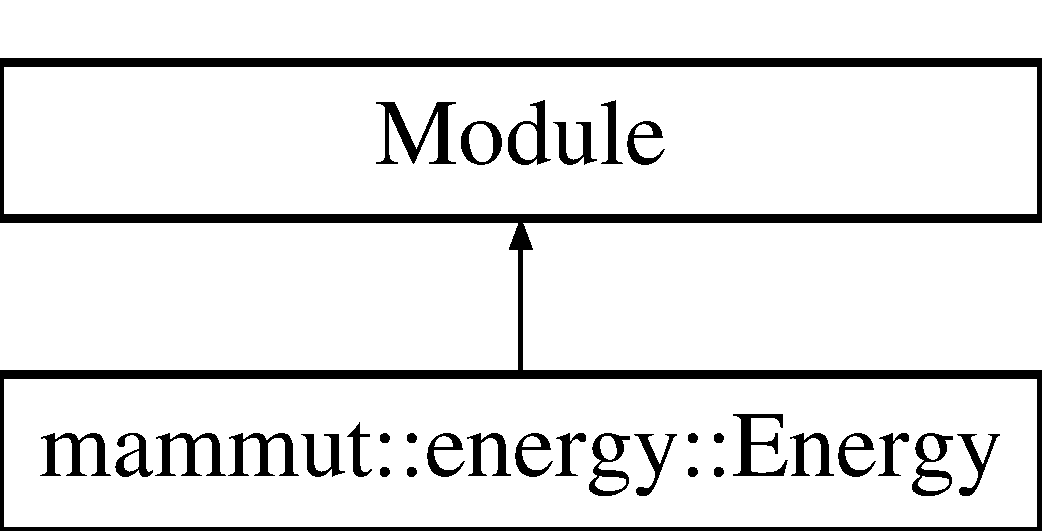
\includegraphics[height=3.000000cm]{classmammut_1_1energy_1_1Energy}
\end{center}
\end{figure}
\subsection*{Public Member Functions}
\begin{DoxyCompactItemize}
\item 
\hyperlink{classmammut_1_1energy_1_1Counter}{Counter} $\ast$ \hyperlink{classmammut_1_1energy_1_1Energy_a5f25777d5bb8e18933d732d52a45ce50}{get\-Counter} () const 
\item 
std\-::vector$<$ Counter\-Type $>$ \hyperlink{classmammut_1_1energy_1_1Energy_a2ef397565802ed9efbe54d782c6917db}{get\-Counters\-Types} () const 
\item 
\hyperlink{classmammut_1_1energy_1_1Counter}{Counter} $\ast$ \hyperlink{classmammut_1_1energy_1_1Energy_a9989f5efbf526e2a5a7bd71ef32c0245}{get\-Counter} (Counter\-Type type) const 
\end{DoxyCompactItemize}


\subsection{Member Function Documentation}
\hypertarget{classmammut_1_1energy_1_1Energy_a5f25777d5bb8e18933d732d52a45ce50}{\index{mammut\-::energy\-::\-Energy@{mammut\-::energy\-::\-Energy}!get\-Counter@{get\-Counter}}
\index{get\-Counter@{get\-Counter}!mammut::energy::Energy@{mammut\-::energy\-::\-Energy}}
\subsubsection[{get\-Counter}]{\setlength{\rightskip}{0pt plus 5cm}{\bf Counter} $\ast$ mammut\-::energy\-::\-Energy\-::get\-Counter (
\begin{DoxyParamCaption}
{}
\end{DoxyParamCaption}
) const}}\label{classmammut_1_1energy_1_1Energy_a5f25777d5bb8e18933d732d52a45ce50}
Returns the most precise energy counter available on this machine, or N\-U\-L\-L if no energy counters are available. \begin{DoxyReturn}{Returns}
The most precise energy counter available on this machine, or N\-U\-L\-L if no energy counters are available. 
\end{DoxyReturn}
\hypertarget{classmammut_1_1energy_1_1Energy_a9989f5efbf526e2a5a7bd71ef32c0245}{\index{mammut\-::energy\-::\-Energy@{mammut\-::energy\-::\-Energy}!get\-Counter@{get\-Counter}}
\index{get\-Counter@{get\-Counter}!mammut::energy::Energy@{mammut\-::energy\-::\-Energy}}
\subsubsection[{get\-Counter}]{\setlength{\rightskip}{0pt plus 5cm}{\bf Counter} $\ast$ mammut\-::energy\-::\-Energy\-::get\-Counter (
\begin{DoxyParamCaption}
\item[{Counter\-Type}]{type}
\end{DoxyParamCaption}
) const}}\label{classmammut_1_1energy_1_1Energy_a9989f5efbf526e2a5a7bd71ef32c0245}
Returns a counter of a specific type if present, N\-U\-L\-L otherwise. 
\begin{DoxyParams}{Parameters}
{\em type} & The type of the counter. \\
\hline
\end{DoxyParams}
\begin{DoxyReturn}{Returns}
A counter of the specified type if present, N\-U\-L\-L otherwise. 
\end{DoxyReturn}
\hypertarget{classmammut_1_1energy_1_1Energy_a2ef397565802ed9efbe54d782c6917db}{\index{mammut\-::energy\-::\-Energy@{mammut\-::energy\-::\-Energy}!get\-Counters\-Types@{get\-Counters\-Types}}
\index{get\-Counters\-Types@{get\-Counters\-Types}!mammut::energy::Energy@{mammut\-::energy\-::\-Energy}}
\subsubsection[{get\-Counters\-Types}]{\setlength{\rightskip}{0pt plus 5cm}std\-::vector$<$ Counter\-Type $>$ mammut\-::energy\-::\-Energy\-::get\-Counters\-Types (
\begin{DoxyParamCaption}
{}
\end{DoxyParamCaption}
) const}}\label{classmammut_1_1energy_1_1Energy_a2ef397565802ed9efbe54d782c6917db}
Returns a vector of counters types available on this machine. The counters are sorted from the most precise to the least precise one. For example, if both C\-P\-Us counter and power plug counter are present, the first element of the vector will be C\-O\-U\-N\-T\-E\-R\-\_\-\-C\-P\-U\-S and the second C\-O\-U\-N\-T\-E\-R\-\_\-\-P\-L\-U\-G. \begin{DoxyReturn}{Returns}
A vector of counters types available on this machine. 
\end{DoxyReturn}


The documentation for this class was generated from the following files\-:\begin{DoxyCompactItemize}
\item 
/home/daniele/\-Code/\-Mammut/mammut/energy/energy.\-hpp\item 
/home/daniele/\-Code/\-Mammut/mammut/energy/energy.\-cpp\end{DoxyCompactItemize}

\hypertarget{structmammut_1_1utils_1_1enumConstRefHolder}{\section{mammut\-:\-:utils\-:\-:enum\-Const\-Ref\-Holder$<$ T $>$ Struct Template Reference}
\label{structmammut_1_1utils_1_1enumConstRefHolder}\index{mammut\-::utils\-::enum\-Const\-Ref\-Holder$<$ T $>$@{mammut\-::utils\-::enum\-Const\-Ref\-Holder$<$ T $>$}}
}
\subsection*{Public Member Functions}
\begin{DoxyCompactItemize}
\item 
\hypertarget{structmammut_1_1utils_1_1enumConstRefHolder_afdca471346bac7da0ea94c6a5df311c4}{{\bfseries enum\-Const\-Ref\-Holder} (T const \&enum\-Val)}\label{structmammut_1_1utils_1_1enumConstRefHolder_afdca471346bac7da0ea94c6a5df311c4}

\end{DoxyCompactItemize}
\subsection*{Public Attributes}
\begin{DoxyCompactItemize}
\item 
\hypertarget{structmammut_1_1utils_1_1enumConstRefHolder_ada294ffa1da728c24a86411bf3860120}{T const \& {\bfseries enum\-Val}}\label{structmammut_1_1utils_1_1enumConstRefHolder_ada294ffa1da728c24a86411bf3860120}

\end{DoxyCompactItemize}


The documentation for this struct was generated from the following file\-:\begin{DoxyCompactItemize}
\item 
/home/daniele/\-Code/\-Mammut/mammut/utils.\-hpp\end{DoxyCompactItemize}

\hypertarget{structmammut_1_1utils_1_1enumRefHolder}{\section{mammut\-:\-:utils\-:\-:enum\-Ref\-Holder$<$ T $>$ Struct Template Reference}
\label{structmammut_1_1utils_1_1enumRefHolder}\index{mammut\-::utils\-::enum\-Ref\-Holder$<$ T $>$@{mammut\-::utils\-::enum\-Ref\-Holder$<$ T $>$}}
}
\subsection*{Public Member Functions}
\begin{DoxyCompactItemize}
\item 
\hypertarget{structmammut_1_1utils_1_1enumRefHolder_a767ffb8c1927f89e40ad83fb07e81029}{{\bfseries enum\-Ref\-Holder} (T \&enum\-Val)}\label{structmammut_1_1utils_1_1enumRefHolder_a767ffb8c1927f89e40ad83fb07e81029}

\end{DoxyCompactItemize}
\subsection*{Public Attributes}
\begin{DoxyCompactItemize}
\item 
\hypertarget{structmammut_1_1utils_1_1enumRefHolder_ae4f40e4a23be3930a6bee62240a8ffc6}{T \& {\bfseries enum\-Val}}\label{structmammut_1_1utils_1_1enumRefHolder_ae4f40e4a23be3930a6bee62240a8ffc6}

\end{DoxyCompactItemize}


The documentation for this struct was generated from the following file\-:\begin{DoxyCompactItemize}
\item 
/home/daniele/\-Code/\-Mammut/mammut/utils.\-hpp\end{DoxyCompactItemize}

\hypertarget{structmammut_1_1utils_1_1enumStrings}{\section{mammut\-:\-:utils\-:\-:enum\-Strings$<$ T $>$ Struct Template Reference}
\label{structmammut_1_1utils_1_1enumStrings}\index{mammut\-::utils\-::enum\-Strings$<$ T $>$@{mammut\-::utils\-::enum\-Strings$<$ T $>$}}
}


{\ttfamily \#include $<$utils.\-hpp$>$}

\subsection*{Static Public Attributes}
\begin{DoxyCompactItemize}
\item 
\hypertarget{structmammut_1_1utils_1_1enumStrings_a2b0c0f1ba01a378a6dbc0b7e292db35c}{static char const $\ast$ {\bfseries data} \mbox{[}$\,$\mbox{]}}\label{structmammut_1_1utils_1_1enumStrings_a2b0c0f1ba01a378a6dbc0b7e292db35c}

\end{DoxyCompactItemize}


\subsection{Detailed Description}
\subsubsection*{template$<$typename T$>$struct mammut\-::utils\-::enum\-Strings$<$ T $>$}

Str$<$-\/$>$Enum mappings Code from \href{http://codereview.stackexchange.com/a/14315}{\tt http\-://codereview.\-stackexchange.\-com/a/14315} 

The documentation for this struct was generated from the following file\-:\begin{DoxyCompactItemize}
\item 
/home/daniele/\-Code/\-Mammut/mammut/utils.\-hpp\end{DoxyCompactItemize}

\hypertarget{classmammut_1_1task_1_1ExecutionUnitLinux}{\section{mammut\-:\-:task\-:\-:Execution\-Unit\-Linux Class Reference}
\label{classmammut_1_1task_1_1ExecutionUnitLinux}\index{mammut\-::task\-::\-Execution\-Unit\-Linux@{mammut\-::task\-::\-Execution\-Unit\-Linux}}
}
Inheritance diagram for mammut\-:\-:task\-:\-:Execution\-Unit\-Linux\-:\begin{figure}[H]
\begin{center}
\leavevmode
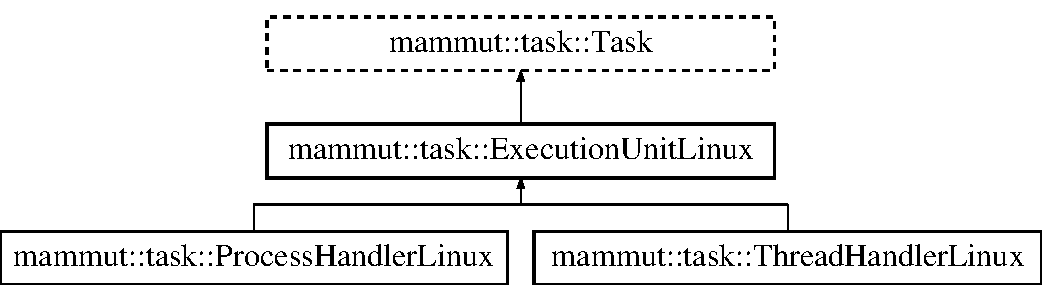
\includegraphics[height=3.000000cm]{classmammut_1_1task_1_1ExecutionUnitLinux}
\end{center}
\end{figure}
\subsection*{Public Member Functions}
\begin{DoxyCompactItemize}
\item 
\hypertarget{classmammut_1_1task_1_1ExecutionUnitLinux_a0b8bcbd22e29b934c8520cd508afaeef}{{\bfseries Execution\-Unit\-Linux} (Task\-Id id, std\-::string path)}\label{classmammut_1_1task_1_1ExecutionUnitLinux_a0b8bcbd22e29b934c8520cd508afaeef}

\item 
\hypertarget{classmammut_1_1task_1_1ExecutionUnitLinux_ab71c03f6a608451a9c6132270871800d}{std\-::string {\bfseries get\-Path} () const }\label{classmammut_1_1task_1_1ExecutionUnitLinux_ab71c03f6a608451a9c6132270871800d}

\item 
bool \hyperlink{classmammut_1_1task_1_1ExecutionUnitLinux_abe366c28b491cda5a42bdc4e76f81273}{get\-Core\-Usage} (double \&core\-Usage) const 
\item 
bool \hyperlink{classmammut_1_1task_1_1ExecutionUnitLinux_a76f3d5ca16cb375e1cd05dcdb580d569}{reset\-Core\-Usage} ()
\item 
bool \hyperlink{classmammut_1_1task_1_1ExecutionUnitLinux_a0c8d351bedcfc82687e2b2c4d7aa3dc3}{get\-Priority} (uint \&priority) const 
\item 
bool \hyperlink{classmammut_1_1task_1_1ExecutionUnitLinux_a10d3890a25520a48de695607730dc297}{set\-Priority} (uint priority) const 
\item 
bool \hyperlink{classmammut_1_1task_1_1ExecutionUnitLinux_ab527ddf71052131babc698c9a7256d3a}{get\-Virtual\-Core\-Id} (topology\-::\-Virtual\-Core\-Id \&virtual\-Core\-Id) const 
\item 
bool \hyperlink{classmammut_1_1task_1_1ExecutionUnitLinux_ab7585761d96e16b2602f9344dacf58a6}{move} (const \hyperlink{classmammut_1_1topology_1_1Cpu}{topology\-::\-Cpu} $\ast$cpu) const 
\item 
bool \hyperlink{classmammut_1_1task_1_1ExecutionUnitLinux_a56288270558b2d8b802e84a8027c3299}{move} (const \hyperlink{classmammut_1_1topology_1_1PhysicalCore}{topology\-::\-Physical\-Core} $\ast$physical\-Core) const 
\item 
bool \hyperlink{classmammut_1_1task_1_1ExecutionUnitLinux_ae948a78fd35c7a6adb83aecf0bb80dab}{move} (const \hyperlink{classmammut_1_1topology_1_1VirtualCore}{topology\-::\-Virtual\-Core} $\ast$virtual\-Core) const 
\item 
bool \hyperlink{classmammut_1_1task_1_1ExecutionUnitLinux_a18bc2f740db5dc7daa7b3750d7f3e3cc}{move} (topology\-::\-Virtual\-Core\-Id virtual\-Core\-Id) const 
\item 
bool \hyperlink{classmammut_1_1task_1_1ExecutionUnitLinux_ab0785f5d6e7fc7dca4c66ccc7871b5d5}{move} (const std\-::vector$<$ const \hyperlink{classmammut_1_1topology_1_1VirtualCore}{topology\-::\-Virtual\-Core} $\ast$ $>$ virtual\-Cores) const 
\item 
virtual bool \hyperlink{classmammut_1_1task_1_1ExecutionUnitLinux_aedac673e0c581fcbfc6b3fb5a38cd81b}{move} (const std\-::vector$<$ topology\-::\-Virtual\-Core\-Id $>$ virtual\-Cores\-Ids) const =0
\end{DoxyCompactItemize}


\subsection{Member Function Documentation}
\hypertarget{classmammut_1_1task_1_1ExecutionUnitLinux_abe366c28b491cda5a42bdc4e76f81273}{\index{mammut\-::task\-::\-Execution\-Unit\-Linux@{mammut\-::task\-::\-Execution\-Unit\-Linux}!get\-Core\-Usage@{get\-Core\-Usage}}
\index{get\-Core\-Usage@{get\-Core\-Usage}!mammut::task::ExecutionUnitLinux@{mammut\-::task\-::\-Execution\-Unit\-Linux}}
\subsubsection[{get\-Core\-Usage}]{\setlength{\rightskip}{0pt plus 5cm}bool mammut\-::task\-::\-Execution\-Unit\-Linux\-::get\-Core\-Usage (
\begin{DoxyParamCaption}
\item[{double \&}]{core\-Usage}
\end{DoxyParamCaption}
) const\hspace{0.3cm}{\ttfamily [virtual]}}}\label{classmammut_1_1task_1_1ExecutionUnitLinux_abe366c28b491cda5a42bdc4e76f81273}
Returns the percentage of time spent by this execution unit on a processing core. The percentage is computed over a period of time spanning from the last call of reset\-Core\-Usage (or from the creation of this object) to the moment of this call. 
\begin{DoxyParams}{Parameters}
{\em core\-Usage} & The percentage of time spent by this execution unit on a processing core. \\
\hline
\end{DoxyParams}
\begin{DoxyReturn}{Returns}
If false is returned, this execution unit is no more active and the call failed. Otherwise, true is returned. 
\end{DoxyReturn}


Implements \hyperlink{classmammut_1_1task_1_1Task_a4649012d8b17e09dc9270b61ad296d91}{mammut\-::task\-::\-Task}.

\hypertarget{classmammut_1_1task_1_1ExecutionUnitLinux_a0c8d351bedcfc82687e2b2c4d7aa3dc3}{\index{mammut\-::task\-::\-Execution\-Unit\-Linux@{mammut\-::task\-::\-Execution\-Unit\-Linux}!get\-Priority@{get\-Priority}}
\index{get\-Priority@{get\-Priority}!mammut::task::ExecutionUnitLinux@{mammut\-::task\-::\-Execution\-Unit\-Linux}}
\subsubsection[{get\-Priority}]{\setlength{\rightskip}{0pt plus 5cm}bool mammut\-::task\-::\-Execution\-Unit\-Linux\-::get\-Priority (
\begin{DoxyParamCaption}
\item[{uint \&}]{priority}
\end{DoxyParamCaption}
) const\hspace{0.3cm}{\ttfamily [virtual]}}}\label{classmammut_1_1task_1_1ExecutionUnitLinux_a0c8d351bedcfc82687e2b2c4d7aa3dc3}
Gets the current priority of this execution unit. 
\begin{DoxyParams}{Parameters}
{\em priority} & The current priority of this execution unit. The higher is the value, the higher is the priority. It will be in the range \mbox{[}M\-A\-M\-M\-U\-T\-\_\-\-P\-R\-O\-C\-E\-S\-S\-\_\-\-P\-R\-I\-O\-R\-I\-T\-Y\-\_\-\-M\-I\-N, M\-A\-M\-M\-U\-T\-\_\-\-P\-R\-O\-C\-E\-S\-S\-\_\-\-P\-R\-I\-O\-R\-I\-T\-Y\-\_\-\-M\-A\-X\mbox{]} \\
\hline
\end{DoxyParams}
\begin{DoxyReturn}{Returns}
If false is returned, this execution unit is no more active and the call failed. Otherwise, true is returned. 
\end{DoxyReturn}


Implements \hyperlink{classmammut_1_1task_1_1Task_a4ff24fb8519aef63e9fd0848f065733d}{mammut\-::task\-::\-Task}.

\hypertarget{classmammut_1_1task_1_1ExecutionUnitLinux_ab527ddf71052131babc698c9a7256d3a}{\index{mammut\-::task\-::\-Execution\-Unit\-Linux@{mammut\-::task\-::\-Execution\-Unit\-Linux}!get\-Virtual\-Core\-Id@{get\-Virtual\-Core\-Id}}
\index{get\-Virtual\-Core\-Id@{get\-Virtual\-Core\-Id}!mammut::task::ExecutionUnitLinux@{mammut\-::task\-::\-Execution\-Unit\-Linux}}
\subsubsection[{get\-Virtual\-Core\-Id}]{\setlength{\rightskip}{0pt plus 5cm}bool mammut\-::task\-::\-Execution\-Unit\-Linux\-::get\-Virtual\-Core\-Id (
\begin{DoxyParamCaption}
\item[{topology\-::\-Virtual\-Core\-Id \&}]{virtual\-Core\-Id}
\end{DoxyParamCaption}
) const\hspace{0.3cm}{\ttfamily [virtual]}}}\label{classmammut_1_1task_1_1ExecutionUnitLinux_ab527ddf71052131babc698c9a7256d3a}
Gets the identifier of the virtual core on which this unit is currently running. 
\begin{DoxyParams}{Parameters}
{\em virtual\-Core\-Id} & The identifier of the virtual core on which this unit is currently running. \\
\hline
\end{DoxyParams}
\begin{DoxyReturn}{Returns}
If false is returned, this execution unit is no more active and the call failed. Otherwise, true is returned. 
\end{DoxyReturn}


Implements \hyperlink{classmammut_1_1task_1_1Task_a8f8b0d63ca29856427735e93b039ea24}{mammut\-::task\-::\-Task}.

\hypertarget{classmammut_1_1task_1_1ExecutionUnitLinux_ab7585761d96e16b2602f9344dacf58a6}{\index{mammut\-::task\-::\-Execution\-Unit\-Linux@{mammut\-::task\-::\-Execution\-Unit\-Linux}!move@{move}}
\index{move@{move}!mammut::task::ExecutionUnitLinux@{mammut\-::task\-::\-Execution\-Unit\-Linux}}
\subsubsection[{move}]{\setlength{\rightskip}{0pt plus 5cm}bool mammut\-::task\-::\-Execution\-Unit\-Linux\-::move (
\begin{DoxyParamCaption}
\item[{const {\bf topology\-::\-Cpu} $\ast$}]{cpu}
\end{DoxyParamCaption}
) const\hspace{0.3cm}{\ttfamily [virtual]}}}\label{classmammut_1_1task_1_1ExecutionUnitLinux_ab7585761d96e16b2602f9344dacf58a6}
Move this execution unit on a specified C\-P\-U. N\-O\-T\-E\-: If executed on a process, all its threads will be moved too. 
\begin{DoxyParams}{Parameters}
{\em cpu} & The C\-P\-U on which this execution unit must be moved. \\
\hline
\end{DoxyParams}
\begin{DoxyReturn}{Returns}
If false is returned, this execution unit is no more active and the call failed. Otherwise, true is returned. 
\end{DoxyReturn}


Implements \hyperlink{classmammut_1_1task_1_1Task_a9f7366c0e1f4c0b9f02e453d18ec41a5}{mammut\-::task\-::\-Task}.

\hypertarget{classmammut_1_1task_1_1ExecutionUnitLinux_a56288270558b2d8b802e84a8027c3299}{\index{mammut\-::task\-::\-Execution\-Unit\-Linux@{mammut\-::task\-::\-Execution\-Unit\-Linux}!move@{move}}
\index{move@{move}!mammut::task::ExecutionUnitLinux@{mammut\-::task\-::\-Execution\-Unit\-Linux}}
\subsubsection[{move}]{\setlength{\rightskip}{0pt plus 5cm}bool mammut\-::task\-::\-Execution\-Unit\-Linux\-::move (
\begin{DoxyParamCaption}
\item[{const {\bf topology\-::\-Physical\-Core} $\ast$}]{physical\-Core}
\end{DoxyParamCaption}
) const\hspace{0.3cm}{\ttfamily [virtual]}}}\label{classmammut_1_1task_1_1ExecutionUnitLinux_a56288270558b2d8b802e84a8027c3299}
Move this execution unit on a specified physical core. N\-O\-T\-E\-: If executed on a process, all its threads will be moved too. 
\begin{DoxyParams}{Parameters}
{\em physical\-Core} & The physical core on which this execution unit must be moved. \\
\hline
\end{DoxyParams}
\begin{DoxyReturn}{Returns}
If false is returned, this execution unit is no more active and the call failed. Otherwise, true is returned. 
\end{DoxyReturn}


Implements \hyperlink{classmammut_1_1task_1_1Task_ae9137276cf4b4440a66b7b310bd51466}{mammut\-::task\-::\-Task}.

\hypertarget{classmammut_1_1task_1_1ExecutionUnitLinux_ae948a78fd35c7a6adb83aecf0bb80dab}{\index{mammut\-::task\-::\-Execution\-Unit\-Linux@{mammut\-::task\-::\-Execution\-Unit\-Linux}!move@{move}}
\index{move@{move}!mammut::task::ExecutionUnitLinux@{mammut\-::task\-::\-Execution\-Unit\-Linux}}
\subsubsection[{move}]{\setlength{\rightskip}{0pt plus 5cm}bool mammut\-::task\-::\-Execution\-Unit\-Linux\-::move (
\begin{DoxyParamCaption}
\item[{const {\bf topology\-::\-Virtual\-Core} $\ast$}]{virtual\-Core}
\end{DoxyParamCaption}
) const\hspace{0.3cm}{\ttfamily [virtual]}}}\label{classmammut_1_1task_1_1ExecutionUnitLinux_ae948a78fd35c7a6adb83aecf0bb80dab}
Move this execution unit on a specified virtual core. N\-O\-T\-E\-: If executed on a process, all its threads will be moved too. 
\begin{DoxyParams}{Parameters}
{\em virtual\-Core} & The virtual core on which this execution unit must be moved. \\
\hline
\end{DoxyParams}
\begin{DoxyReturn}{Returns}
If false is returned, this execution unit is no more active and the call failed. Otherwise, true is returned. 
\end{DoxyReturn}


Implements \hyperlink{classmammut_1_1task_1_1Task_a10937944c3534c4b5a21b584c9ceafb8}{mammut\-::task\-::\-Task}.

\hypertarget{classmammut_1_1task_1_1ExecutionUnitLinux_a18bc2f740db5dc7daa7b3750d7f3e3cc}{\index{mammut\-::task\-::\-Execution\-Unit\-Linux@{mammut\-::task\-::\-Execution\-Unit\-Linux}!move@{move}}
\index{move@{move}!mammut::task::ExecutionUnitLinux@{mammut\-::task\-::\-Execution\-Unit\-Linux}}
\subsubsection[{move}]{\setlength{\rightskip}{0pt plus 5cm}bool mammut\-::task\-::\-Execution\-Unit\-Linux\-::move (
\begin{DoxyParamCaption}
\item[{topology\-::\-Virtual\-Core\-Id}]{virtual\-Core\-Id}
\end{DoxyParamCaption}
) const\hspace{0.3cm}{\ttfamily [virtual]}}}\label{classmammut_1_1task_1_1ExecutionUnitLinux_a18bc2f740db5dc7daa7b3750d7f3e3cc}
Move this execution unit on a specified virtual core. N\-O\-T\-E\-: If executed on a process, all its threads will be moved too. 
\begin{DoxyParams}{Parameters}
{\em virtual\-Core\-Id} & The identifier of the virtual core on which this execution unit must be moved. \\
\hline
\end{DoxyParams}
\begin{DoxyReturn}{Returns}
If false is returned, this execution unit is no more active and the call failed. Otherwise, true is returned. 
\end{DoxyReturn}


Implements \hyperlink{classmammut_1_1task_1_1Task_a461a62415be252aaf4868ee781b09220}{mammut\-::task\-::\-Task}.

\hypertarget{classmammut_1_1task_1_1ExecutionUnitLinux_ab0785f5d6e7fc7dca4c66ccc7871b5d5}{\index{mammut\-::task\-::\-Execution\-Unit\-Linux@{mammut\-::task\-::\-Execution\-Unit\-Linux}!move@{move}}
\index{move@{move}!mammut::task::ExecutionUnitLinux@{mammut\-::task\-::\-Execution\-Unit\-Linux}}
\subsubsection[{move}]{\setlength{\rightskip}{0pt plus 5cm}bool mammut\-::task\-::\-Execution\-Unit\-Linux\-::move (
\begin{DoxyParamCaption}
\item[{const std\-::vector$<$ const {\bf topology\-::\-Virtual\-Core} $\ast$ $>$}]{virtual\-Cores}
\end{DoxyParamCaption}
) const\hspace{0.3cm}{\ttfamily [virtual]}}}\label{classmammut_1_1task_1_1ExecutionUnitLinux_ab0785f5d6e7fc7dca4c66ccc7871b5d5}
Move this execution unit on a set of specified virtual cores. 
\begin{DoxyParams}{Parameters}
{\em virtual\-Cores} & The virtual cores on which this execution unit must be moved. \\
\hline
\end{DoxyParams}
\begin{DoxyReturn}{Returns}
If false is returned, this execution unit is no more active and the call failed. Otherwise, true is returned. 
\end{DoxyReturn}


Implements \hyperlink{classmammut_1_1task_1_1Task_afb35378fa3ebdbb92aa2875530b9cb64}{mammut\-::task\-::\-Task}.

\hypertarget{classmammut_1_1task_1_1ExecutionUnitLinux_aedac673e0c581fcbfc6b3fb5a38cd81b}{\index{mammut\-::task\-::\-Execution\-Unit\-Linux@{mammut\-::task\-::\-Execution\-Unit\-Linux}!move@{move}}
\index{move@{move}!mammut::task::ExecutionUnitLinux@{mammut\-::task\-::\-Execution\-Unit\-Linux}}
\subsubsection[{move}]{\setlength{\rightskip}{0pt plus 5cm}virtual bool mammut\-::task\-::\-Execution\-Unit\-Linux\-::move (
\begin{DoxyParamCaption}
\item[{const std\-::vector$<$ topology\-::\-Virtual\-Core\-Id $>$}]{virtual\-Cores\-Ids}
\end{DoxyParamCaption}
) const\hspace{0.3cm}{\ttfamily [pure virtual]}}}\label{classmammut_1_1task_1_1ExecutionUnitLinux_aedac673e0c581fcbfc6b3fb5a38cd81b}
Move this execution unit on a set of specified virtual cores. 
\begin{DoxyParams}{Parameters}
{\em virtual\-Cores\-Ids} & The identifiers of the virtual cores on which this execution unit must be moved. \\
\hline
\end{DoxyParams}
\begin{DoxyReturn}{Returns}
If false is returned, this execution unit is no more active and the call failed. Otherwise, true is returned. 
\end{DoxyReturn}


Implements \hyperlink{classmammut_1_1task_1_1Task_af6bd70528163acb0e1c5becc7bdca326}{mammut\-::task\-::\-Task}.



Implemented in \hyperlink{classmammut_1_1task_1_1ProcessHandlerLinux_afe9e66ee6d87efd57c9bbfcc51ec0db6}{mammut\-::task\-::\-Process\-Handler\-Linux}, and \hyperlink{classmammut_1_1task_1_1ThreadHandlerLinux_a7ecc4783d78c0fdfc337800598b0165c}{mammut\-::task\-::\-Thread\-Handler\-Linux}.

\hypertarget{classmammut_1_1task_1_1ExecutionUnitLinux_a76f3d5ca16cb375e1cd05dcdb580d569}{\index{mammut\-::task\-::\-Execution\-Unit\-Linux@{mammut\-::task\-::\-Execution\-Unit\-Linux}!reset\-Core\-Usage@{reset\-Core\-Usage}}
\index{reset\-Core\-Usage@{reset\-Core\-Usage}!mammut::task::ExecutionUnitLinux@{mammut\-::task\-::\-Execution\-Unit\-Linux}}
\subsubsection[{reset\-Core\-Usage}]{\setlength{\rightskip}{0pt plus 5cm}bool mammut\-::task\-::\-Execution\-Unit\-Linux\-::reset\-Core\-Usage (
\begin{DoxyParamCaption}
{}
\end{DoxyParamCaption}
)\hspace{0.3cm}{\ttfamily [virtual]}}}\label{classmammut_1_1task_1_1ExecutionUnitLinux_a76f3d5ca16cb375e1cd05dcdb580d569}
Resets the counter for core usage percentage computation. \begin{DoxyReturn}{Returns}
If false is returned, this execution unit is no more active and the call failed. Otherwise, true is returned. 
\end{DoxyReturn}


Implements \hyperlink{classmammut_1_1task_1_1Task_a07b164a46a147eb76af005fa23e39826}{mammut\-::task\-::\-Task}.

\hypertarget{classmammut_1_1task_1_1ExecutionUnitLinux_a10d3890a25520a48de695607730dc297}{\index{mammut\-::task\-::\-Execution\-Unit\-Linux@{mammut\-::task\-::\-Execution\-Unit\-Linux}!set\-Priority@{set\-Priority}}
\index{set\-Priority@{set\-Priority}!mammut::task::ExecutionUnitLinux@{mammut\-::task\-::\-Execution\-Unit\-Linux}}
\subsubsection[{set\-Priority}]{\setlength{\rightskip}{0pt plus 5cm}bool mammut\-::task\-::\-Execution\-Unit\-Linux\-::set\-Priority (
\begin{DoxyParamCaption}
\item[{uint}]{priority}
\end{DoxyParamCaption}
) const\hspace{0.3cm}{\ttfamily [virtual]}}}\label{classmammut_1_1task_1_1ExecutionUnitLinux_a10d3890a25520a48de695607730dc297}
Sets the priority of this execution unit. N\-O\-T\-E\-: If executed on a process, the priority of all its thread will be changed too. N\-O\-T\-E\-: It may require privileged rights. 
\begin{DoxyParams}{Parameters}
{\em priority} & The priority of this execution unit. The higher is the value, the higher is the priority. It must be in the range \mbox{[}M\-A\-M\-M\-U\-T\-\_\-\-P\-R\-O\-C\-E\-S\-S\-\_\-\-P\-R\-I\-O\-R\-I\-T\-Y\-\_\-\-M\-I\-N, M\-A\-M\-M\-U\-T\-\_\-\-P\-R\-O\-C\-E\-S\-S\-\_\-\-P\-R\-I\-O\-R\-I\-T\-Y\-\_\-\-M\-A\-X\mbox{]} \\
\hline
\end{DoxyParams}
\begin{DoxyReturn}{Returns}
If false is returned, the priority value is outside the allowed range or this execution unit is no more active and the call failed. Otherwise, true is returned. 
\end{DoxyReturn}


Implements \hyperlink{classmammut_1_1task_1_1Task_a6ca8b0fb237d41bdae18dd5d98ed4012}{mammut\-::task\-::\-Task}.



The documentation for this class was generated from the following files\-:\begin{DoxyCompactItemize}
\item 
/home/daniele/\-Code/\-Mammut/mammut/task/task-\/linux.\-hpp\item 
/home/daniele/\-Code/\-Mammut/mammut/task/task-\/linux.\-cpp\end{DoxyCompactItemize}

\hypertarget{classmammut_1_1energy_1_1JoulesCpu}{\section{mammut\-:\-:energy\-:\-:Joules\-Cpu Class Reference}
\label{classmammut_1_1energy_1_1JoulesCpu}\index{mammut\-::energy\-::\-Joules\-Cpu@{mammut\-::energy\-::\-Joules\-Cpu}}
}


Represents the values that can be read from a Cpu energy counter.  




{\ttfamily \#include $<$energy.\-hpp$>$}

\subsection*{Public Member Functions}
\begin{DoxyCompactItemize}
\item 
\hypertarget{classmammut_1_1energy_1_1JoulesCpu_ae4fd0bc3cfe0e131d94d69858bdd7892}{{\bfseries Joules\-Cpu} (Joules cpu, Joules cores, Joules graphic, Joules dram)}\label{classmammut_1_1energy_1_1JoulesCpu_ae4fd0bc3cfe0e131d94d69858bdd7892}

\item 
void \hyperlink{classmammut_1_1energy_1_1JoulesCpu_a7a6e400b23e26d0701f314b5fe1b21f5}{zero} ()
\item 
\hypertarget{classmammut_1_1energy_1_1JoulesCpu_a61c5200a76004b09dd1253ed32f6a9ac}{void {\bfseries swap} (\hyperlink{classmammut_1_1energy_1_1JoulesCpu}{Joules\-Cpu} \&x)}\label{classmammut_1_1energy_1_1JoulesCpu_a61c5200a76004b09dd1253ed32f6a9ac}

\item 
\hypertarget{classmammut_1_1energy_1_1JoulesCpu_a6ac87108c47399e37b9af515d8073b9b}{\hyperlink{classmammut_1_1energy_1_1JoulesCpu}{Joules\-Cpu} \& {\bfseries operator=} (\hyperlink{classmammut_1_1energy_1_1JoulesCpu}{Joules\-Cpu} rhs)}\label{classmammut_1_1energy_1_1JoulesCpu_a6ac87108c47399e37b9af515d8073b9b}

\item 
\hypertarget{classmammut_1_1energy_1_1JoulesCpu_afb350f44d1ed7623139e10dede505630}{\hyperlink{classmammut_1_1energy_1_1JoulesCpu}{Joules\-Cpu} \& {\bfseries operator+=} (const \hyperlink{classmammut_1_1energy_1_1JoulesCpu}{Joules\-Cpu} \&rhs)}\label{classmammut_1_1energy_1_1JoulesCpu_afb350f44d1ed7623139e10dede505630}

\item 
\hypertarget{classmammut_1_1energy_1_1JoulesCpu_a6b20192aa4e6be35d914f9cce62f768e}{\hyperlink{classmammut_1_1energy_1_1JoulesCpu}{Joules\-Cpu} \& {\bfseries operator-\/=} (const \hyperlink{classmammut_1_1energy_1_1JoulesCpu}{Joules\-Cpu} \&rhs)}\label{classmammut_1_1energy_1_1JoulesCpu_a6b20192aa4e6be35d914f9cce62f768e}

\item 
\hypertarget{classmammut_1_1energy_1_1JoulesCpu_a8721e6f586965be304d1183cb9f346a6}{\hyperlink{classmammut_1_1energy_1_1JoulesCpu}{Joules\-Cpu} \& {\bfseries operator$\ast$=} (const \hyperlink{classmammut_1_1energy_1_1JoulesCpu}{Joules\-Cpu} \&rhs)}\label{classmammut_1_1energy_1_1JoulesCpu_a8721e6f586965be304d1183cb9f346a6}

\item 
\hypertarget{classmammut_1_1energy_1_1JoulesCpu_a8197d020ac5a0dcfc6ba3ce52d54e8ae}{\hyperlink{classmammut_1_1energy_1_1JoulesCpu}{Joules\-Cpu} \& {\bfseries operator/=} (const \hyperlink{classmammut_1_1energy_1_1JoulesCpu}{Joules\-Cpu} \&rhs)}\label{classmammut_1_1energy_1_1JoulesCpu_a8197d020ac5a0dcfc6ba3ce52d54e8ae}

\item 
\hypertarget{classmammut_1_1energy_1_1JoulesCpu_a3a62f9fbff1613c13df0dcac7d717f41}{\hyperlink{classmammut_1_1energy_1_1JoulesCpu}{Joules\-Cpu} {\bfseries operator/=} (double x)}\label{classmammut_1_1energy_1_1JoulesCpu_a3a62f9fbff1613c13df0dcac7d717f41}

\item 
\hypertarget{classmammut_1_1energy_1_1JoulesCpu_ae9c3b9fadb2004a77e77456afbdb49d7}{\hyperlink{classmammut_1_1energy_1_1JoulesCpu}{Joules\-Cpu} {\bfseries operator$\ast$=} (double x)}\label{classmammut_1_1energy_1_1JoulesCpu_ae9c3b9fadb2004a77e77456afbdb49d7}

\end{DoxyCompactItemize}
\subsection*{Public Attributes}
\begin{DoxyCompactItemize}
\item 
\hypertarget{classmammut_1_1energy_1_1JoulesCpu_a406c57faafd2a94f605fc011f34b1b09}{Joules {\bfseries cpu}}\label{classmammut_1_1energy_1_1JoulesCpu_a406c57faafd2a94f605fc011f34b1b09}

\item 
\hypertarget{classmammut_1_1energy_1_1JoulesCpu_a00f80dc44f7ccbef2c27042253182b26}{Joules {\bfseries cores}}\label{classmammut_1_1energy_1_1JoulesCpu_a00f80dc44f7ccbef2c27042253182b26}

\item 
\hypertarget{classmammut_1_1energy_1_1JoulesCpu_ae83ef5e6029300e9a784f92391e325d0}{Joules {\bfseries graphic}}\label{classmammut_1_1energy_1_1JoulesCpu_ae83ef5e6029300e9a784f92391e325d0}

\item 
\hypertarget{classmammut_1_1energy_1_1JoulesCpu_a635372e3958cf576dd9d5076b7636ad6}{Joules {\bfseries dram}}\label{classmammut_1_1energy_1_1JoulesCpu_a635372e3958cf576dd9d5076b7636ad6}

\end{DoxyCompactItemize}
\subsection*{Friends}
\begin{DoxyCompactItemize}
\item 
\hypertarget{classmammut_1_1energy_1_1JoulesCpu_ae94a8fa2c7633d8dc71580f262de35b4}{std\-::ostream \& {\bfseries operator$<$$<$} (std\-::ostream \&os, const \hyperlink{classmammut_1_1energy_1_1JoulesCpu}{Joules\-Cpu} \&obj)}\label{classmammut_1_1energy_1_1JoulesCpu_ae94a8fa2c7633d8dc71580f262de35b4}

\end{DoxyCompactItemize}


\subsection{Detailed Description}
Represents the values that can be read from a Cpu energy counter. 

\subsection{Member Function Documentation}
\hypertarget{classmammut_1_1energy_1_1JoulesCpu_a7a6e400b23e26d0701f314b5fe1b21f5}{\index{mammut\-::energy\-::\-Joules\-Cpu@{mammut\-::energy\-::\-Joules\-Cpu}!zero@{zero}}
\index{zero@{zero}!mammut::energy::JoulesCpu@{mammut\-::energy\-::\-Joules\-Cpu}}
\subsubsection[{zero}]{\setlength{\rightskip}{0pt plus 5cm}void mammut\-::energy\-::\-Joules\-Cpu\-::zero (
\begin{DoxyParamCaption}
{}
\end{DoxyParamCaption}
)\hspace{0.3cm}{\ttfamily [inline]}}}\label{classmammut_1_1energy_1_1JoulesCpu_a7a6e400b23e26d0701f314b5fe1b21f5}
Zeroes its content. 

The documentation for this class was generated from the following file\-:\begin{DoxyCompactItemize}
\item 
/home/daniele/\-Code/\-Mammut/mammut/energy/energy.\-hpp\end{DoxyCompactItemize}

\hypertarget{classmammut_1_1utils_1_1Lock}{\section{mammut\-:\-:utils\-:\-:Lock Class Reference}
\label{classmammut_1_1utils_1_1Lock}\index{mammut\-::utils\-::\-Lock@{mammut\-::utils\-::\-Lock}}
}
Inheritance diagram for mammut\-:\-:utils\-:\-:Lock\-:\begin{figure}[H]
\begin{center}
\leavevmode
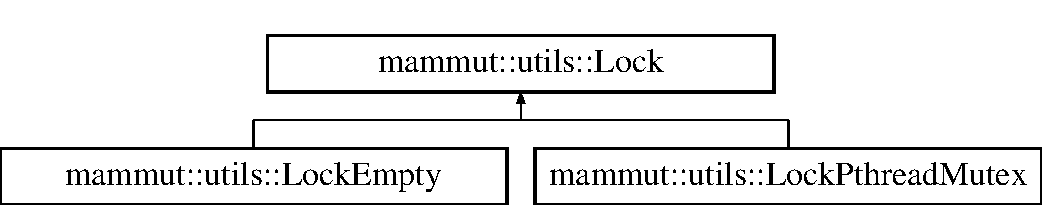
\includegraphics[height=2.000000cm]{classmammut_1_1utils_1_1Lock}
\end{center}
\end{figure}
\subsection*{Public Member Functions}
\begin{DoxyCompactItemize}
\item 
\hypertarget{classmammut_1_1utils_1_1Lock_a175578977267834347950e47fb7cbf4f}{virtual void {\bfseries lock} ()=0}\label{classmammut_1_1utils_1_1Lock_a175578977267834347950e47fb7cbf4f}

\item 
\hypertarget{classmammut_1_1utils_1_1Lock_a857cceda31f27336f227ab3b2e490467}{virtual void {\bfseries unlock} ()=0}\label{classmammut_1_1utils_1_1Lock_a857cceda31f27336f227ab3b2e490467}

\end{DoxyCompactItemize}


The documentation for this class was generated from the following files\-:\begin{DoxyCompactItemize}
\item 
/home/daniele/\-Code/\-Mammut/mammut/utils.\-hpp\item 
/home/daniele/\-Code/\-Mammut/mammut/utils.\-cpp\end{DoxyCompactItemize}

\hypertarget{classmammut_1_1utils_1_1LockEmpty}{\section{mammut\-:\-:utils\-:\-:Lock\-Empty Class Reference}
\label{classmammut_1_1utils_1_1LockEmpty}\index{mammut\-::utils\-::\-Lock\-Empty@{mammut\-::utils\-::\-Lock\-Empty}}
}
Inheritance diagram for mammut\-:\-:utils\-:\-:Lock\-Empty\-:\begin{figure}[H]
\begin{center}
\leavevmode
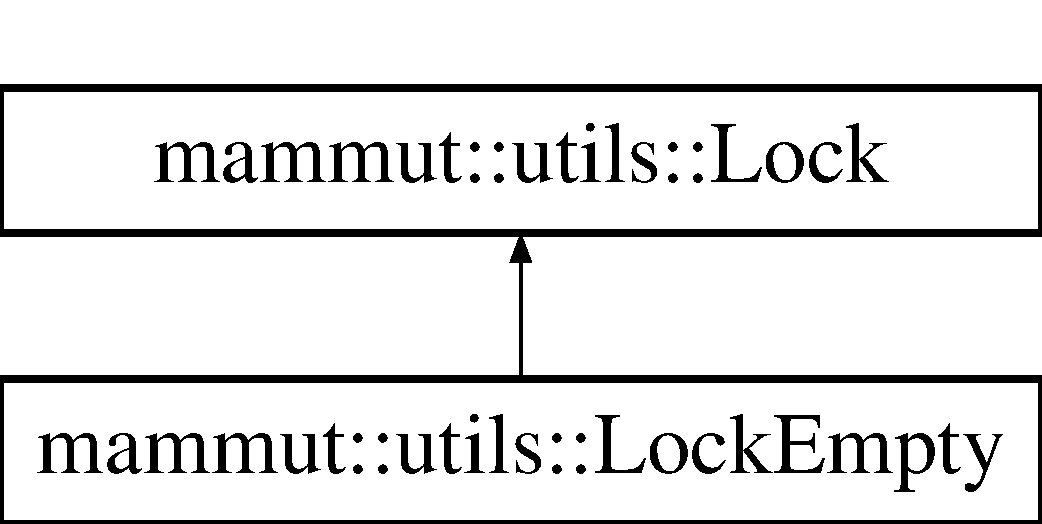
\includegraphics[height=2.000000cm]{classmammut_1_1utils_1_1LockEmpty}
\end{center}
\end{figure}
\subsection*{Public Member Functions}
\begin{DoxyCompactItemize}
\item 
\hypertarget{classmammut_1_1utils_1_1LockEmpty_aa91e955cd6891b5e7301b05e67eef031}{void {\bfseries lock} ()}\label{classmammut_1_1utils_1_1LockEmpty_aa91e955cd6891b5e7301b05e67eef031}

\item 
\hypertarget{classmammut_1_1utils_1_1LockEmpty_a798c17ef0a05e2d4cf70aa193fba93db}{void {\bfseries unlock} ()}\label{classmammut_1_1utils_1_1LockEmpty_a798c17ef0a05e2d4cf70aa193fba93db}

\end{DoxyCompactItemize}


The documentation for this class was generated from the following files\-:\begin{DoxyCompactItemize}
\item 
/home/daniele/\-Code/\-Mammut/mammut/utils.\-hpp\item 
/home/daniele/\-Code/\-Mammut/mammut/utils.\-cpp\end{DoxyCompactItemize}

\hypertarget{classmammut_1_1utils_1_1LockPthreadMutex}{\section{mammut\-:\-:utils\-:\-:Lock\-Pthread\-Mutex Class Reference}
\label{classmammut_1_1utils_1_1LockPthreadMutex}\index{mammut\-::utils\-::\-Lock\-Pthread\-Mutex@{mammut\-::utils\-::\-Lock\-Pthread\-Mutex}}
}
Inheritance diagram for mammut\-:\-:utils\-:\-:Lock\-Pthread\-Mutex\-:\begin{figure}[H]
\begin{center}
\leavevmode
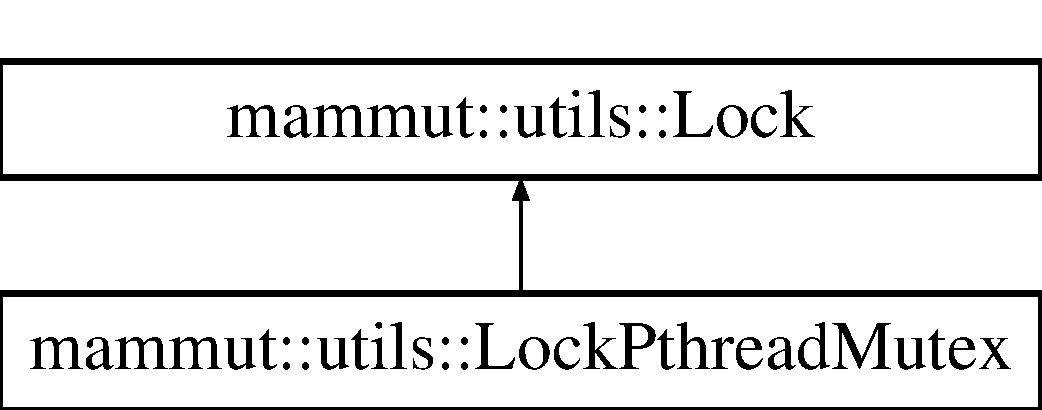
\includegraphics[height=2.000000cm]{classmammut_1_1utils_1_1LockPthreadMutex}
\end{center}
\end{figure}
\subsection*{Public Member Functions}
\begin{DoxyCompactItemize}
\item 
\hypertarget{classmammut_1_1utils_1_1LockPthreadMutex_a4165efbee89fe51a5511679bdfa4b56b}{void {\bfseries lock} ()}\label{classmammut_1_1utils_1_1LockPthreadMutex_a4165efbee89fe51a5511679bdfa4b56b}

\item 
\hypertarget{classmammut_1_1utils_1_1LockPthreadMutex_a195edaf5469a611491cd0b3afe6c43e0}{void {\bfseries unlock} ()}\label{classmammut_1_1utils_1_1LockPthreadMutex_a195edaf5469a611491cd0b3afe6c43e0}

\item 
\hypertarget{classmammut_1_1utils_1_1LockPthreadMutex_a7c4b461e9e687a7676bdb444ea802dc1}{pthread\-\_\-mutex\-\_\-t $\ast$ {\bfseries get\-Lock} ()}\label{classmammut_1_1utils_1_1LockPthreadMutex_a7c4b461e9e687a7676bdb444ea802dc1}

\end{DoxyCompactItemize}


The documentation for this class was generated from the following files\-:\begin{DoxyCompactItemize}
\item 
/home/daniele/\-Code/\-Mammut/mammut/utils.\-hpp\item 
/home/daniele/\-Code/\-Mammut/mammut/utils.\-cpp\end{DoxyCompactItemize}

\hypertarget{classmammut_1_1Mammut}{\section{mammut\-:\-:Mammut Class Reference}
\label{classmammut_1_1Mammut}\index{mammut\-::\-Mammut@{mammut\-::\-Mammut}}
}
\subsection*{Public Member Functions}
\begin{DoxyCompactItemize}
\item 
\hyperlink{classmammut_1_1Mammut_a9969f1d5c17e793629a9054523e47078}{Mammut} (Communicator $\ast$const communicator=N\-U\-L\-L)
\item 
\hyperlink{classmammut_1_1Mammut_acdb713bc158da89c42e07f936e2bdaf1}{Mammut} (const \hyperlink{classmammut_1_1Mammut}{Mammut} \&other)
\item 
\hyperlink{classmammut_1_1Mammut_a7de89ade46172cb5e10ee622cf03cf62}{$\sim$\-Mammut} ()
\item 
\hyperlink{classmammut_1_1Mammut}{Mammut} \& \hyperlink{classmammut_1_1Mammut_ae82723eb711875162e875ed399db3358}{operator=} (const \hyperlink{classmammut_1_1Mammut}{Mammut} \&other)
\item 
\hyperlink{classmammut_1_1cpufreq_1_1CpuFreq}{cpufreq\-::\-Cpu\-Freq} $\ast$ \hyperlink{classmammut_1_1Mammut_a6a630059fc041b5b1cf04666231209da}{get\-Instance\-Cpu\-Freq} () const 
\item 
\hyperlink{classmammut_1_1energy_1_1Energy}{energy\-::\-Energy} $\ast$ \hyperlink{classmammut_1_1Mammut_a945bd8e9269bb431a6c33dc20f635c7c}{get\-Instance\-Energy} () const 
\item 
\hyperlink{classmammut_1_1task_1_1TasksManager}{task\-::\-Tasks\-Manager} $\ast$ \hyperlink{classmammut_1_1Mammut_aa4ad17d8a6cd327cf6ef874aed2fd4b0}{get\-Instance\-Task} () const 
\item 
\hyperlink{classmammut_1_1topology_1_1Topology}{topology\-::\-Topology} $\ast$ \hyperlink{classmammut_1_1Mammut_a8833e0d9c1fea917833efdfc9dcc5343}{get\-Instance\-Topology} () const 
\end{DoxyCompactItemize}


\subsection{Constructor \& Destructor Documentation}
\hypertarget{classmammut_1_1Mammut_a9969f1d5c17e793629a9054523e47078}{\index{mammut\-::\-Mammut@{mammut\-::\-Mammut}!Mammut@{Mammut}}
\index{Mammut@{Mammut}!mammut::Mammut@{mammut\-::\-Mammut}}
\subsubsection[{Mammut}]{\setlength{\rightskip}{0pt plus 5cm}mammut\-::\-Mammut\-::\-Mammut (
\begin{DoxyParamCaption}
\item[{Communicator $\ast$const}]{communicator = {\ttfamily NULL}}
\end{DoxyParamCaption}
)}}\label{classmammut_1_1Mammut_a9969f1d5c17e793629a9054523e47078}
Creates a mammut handler. 
\begin{DoxyParams}{Parameters}
{\em communicator} & If different from N\-U\-L\-L, all the modules will interact with a remote machine specified in the communicator. \\
\hline
\end{DoxyParams}
\hypertarget{classmammut_1_1Mammut_acdb713bc158da89c42e07f936e2bdaf1}{\index{mammut\-::\-Mammut@{mammut\-::\-Mammut}!Mammut@{Mammut}}
\index{Mammut@{Mammut}!mammut::Mammut@{mammut\-::\-Mammut}}
\subsubsection[{Mammut}]{\setlength{\rightskip}{0pt plus 5cm}mammut\-::\-Mammut\-::\-Mammut (
\begin{DoxyParamCaption}
\item[{const {\bf Mammut} \&}]{other}
\end{DoxyParamCaption}
)}}\label{classmammut_1_1Mammut_acdb713bc158da89c42e07f936e2bdaf1}
Copy constructor. 
\begin{DoxyParams}{Parameters}
{\em other} & The object to copy from. \\
\hline
\end{DoxyParams}
\hypertarget{classmammut_1_1Mammut_a7de89ade46172cb5e10ee622cf03cf62}{\index{mammut\-::\-Mammut@{mammut\-::\-Mammut}!$\sim$\-Mammut@{$\sim$\-Mammut}}
\index{$\sim$\-Mammut@{$\sim$\-Mammut}!mammut::Mammut@{mammut\-::\-Mammut}}
\subsubsection[{$\sim$\-Mammut}]{\setlength{\rightskip}{0pt plus 5cm}mammut\-::\-Mammut\-::$\sim$\-Mammut (
\begin{DoxyParamCaption}
{}
\end{DoxyParamCaption}
)}}\label{classmammut_1_1Mammut_a7de89ade46172cb5e10ee622cf03cf62}
Destroyes this mammut instance. 

\subsection{Member Function Documentation}
\hypertarget{classmammut_1_1Mammut_a6a630059fc041b5b1cf04666231209da}{\index{mammut\-::\-Mammut@{mammut\-::\-Mammut}!get\-Instance\-Cpu\-Freq@{get\-Instance\-Cpu\-Freq}}
\index{get\-Instance\-Cpu\-Freq@{get\-Instance\-Cpu\-Freq}!mammut::Mammut@{mammut\-::\-Mammut}}
\subsubsection[{get\-Instance\-Cpu\-Freq}]{\setlength{\rightskip}{0pt plus 5cm}{\bf cpufreq\-::\-Cpu\-Freq}$\ast$ mammut\-::\-Mammut\-::get\-Instance\-Cpu\-Freq (
\begin{DoxyParamCaption}
{}
\end{DoxyParamCaption}
) const}}\label{classmammut_1_1Mammut_a6a630059fc041b5b1cf04666231209da}
Returns an instance of the Cpu\-Freq module. \begin{DoxyReturn}{Returns}
An instance of the Cpu\-Freq module. 
\end{DoxyReturn}
\hypertarget{classmammut_1_1Mammut_a945bd8e9269bb431a6c33dc20f635c7c}{\index{mammut\-::\-Mammut@{mammut\-::\-Mammut}!get\-Instance\-Energy@{get\-Instance\-Energy}}
\index{get\-Instance\-Energy@{get\-Instance\-Energy}!mammut::Mammut@{mammut\-::\-Mammut}}
\subsubsection[{get\-Instance\-Energy}]{\setlength{\rightskip}{0pt plus 5cm}{\bf energy\-::\-Energy}$\ast$ mammut\-::\-Mammut\-::get\-Instance\-Energy (
\begin{DoxyParamCaption}
{}
\end{DoxyParamCaption}
) const}}\label{classmammut_1_1Mammut_a945bd8e9269bb431a6c33dc20f635c7c}
Returns an instance of the Energy module. \begin{DoxyReturn}{Returns}
An instance of the Energy module. 
\end{DoxyReturn}
\hypertarget{classmammut_1_1Mammut_aa4ad17d8a6cd327cf6ef874aed2fd4b0}{\index{mammut\-::\-Mammut@{mammut\-::\-Mammut}!get\-Instance\-Task@{get\-Instance\-Task}}
\index{get\-Instance\-Task@{get\-Instance\-Task}!mammut::Mammut@{mammut\-::\-Mammut}}
\subsubsection[{get\-Instance\-Task}]{\setlength{\rightskip}{0pt plus 5cm}{\bf task\-::\-Tasks\-Manager}$\ast$ mammut\-::\-Mammut\-::get\-Instance\-Task (
\begin{DoxyParamCaption}
{}
\end{DoxyParamCaption}
) const}}\label{classmammut_1_1Mammut_aa4ad17d8a6cd327cf6ef874aed2fd4b0}
Returns an instance of the Task module. \begin{DoxyReturn}{Returns}
An instance of the Task module. 
\end{DoxyReturn}
\hypertarget{classmammut_1_1Mammut_a8833e0d9c1fea917833efdfc9dcc5343}{\index{mammut\-::\-Mammut@{mammut\-::\-Mammut}!get\-Instance\-Topology@{get\-Instance\-Topology}}
\index{get\-Instance\-Topology@{get\-Instance\-Topology}!mammut::Mammut@{mammut\-::\-Mammut}}
\subsubsection[{get\-Instance\-Topology}]{\setlength{\rightskip}{0pt plus 5cm}{\bf topology\-::\-Topology}$\ast$ mammut\-::\-Mammut\-::get\-Instance\-Topology (
\begin{DoxyParamCaption}
{}
\end{DoxyParamCaption}
) const}}\label{classmammut_1_1Mammut_a8833e0d9c1fea917833efdfc9dcc5343}
Returns an instance of the Topology module. \begin{DoxyReturn}{Returns}
An instance of the Topology module. 
\end{DoxyReturn}
\hypertarget{classmammut_1_1Mammut_ae82723eb711875162e875ed399db3358}{\index{mammut\-::\-Mammut@{mammut\-::\-Mammut}!operator=@{operator=}}
\index{operator=@{operator=}!mammut::Mammut@{mammut\-::\-Mammut}}
\subsubsection[{operator=}]{\setlength{\rightskip}{0pt plus 5cm}{\bf Mammut}\& mammut\-::\-Mammut\-::operator= (
\begin{DoxyParamCaption}
\item[{const {\bf Mammut} \&}]{other}
\end{DoxyParamCaption}
)}}\label{classmammut_1_1Mammut_ae82723eb711875162e875ed399db3358}
Assigns an instance of mammut to another one. 
\begin{DoxyParams}{Parameters}
{\em other} & The other instance. \\
\hline
\end{DoxyParams}


The documentation for this class was generated from the following file\-:\begin{DoxyCompactItemize}
\item 
/home/daniele/\-Code/\-Mammut/mammut/mammut.\-hpp\end{DoxyCompactItemize}

\hypertarget{classmammut_1_1Module}{\section{mammut\-:\-:Module Class Reference}
\label{classmammut_1_1Module}\index{mammut\-::\-Module@{mammut\-::\-Module}}
}
Inheritance diagram for mammut\-:\-:Module\-:\begin{figure}[H]
\begin{center}
\leavevmode
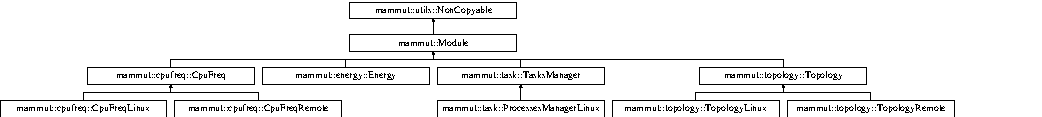
\includegraphics[height=1.568627cm]{classmammut_1_1Module}
\end{center}
\end{figure}
\subsection*{Friends}
\begin{DoxyCompactItemize}
\item 
\hypertarget{classmammut_1_1Module_a228d7ba30b07bfe0230ce7ffb257944f}{class {\bfseries \-::mammut\-::\-Servant}}\label{classmammut_1_1Module_a228d7ba30b07bfe0230ce7ffb257944f}

\end{DoxyCompactItemize}


The documentation for this class was generated from the following file\-:\begin{DoxyCompactItemize}
\item 
/home/daniele/\-Code/\-Mammut/mammut/module.\-hpp\end{DoxyCompactItemize}

\hypertarget{classmammut_1_1utils_1_1Monitor}{\section{mammut\-:\-:utils\-:\-:Monitor Class Reference}
\label{classmammut_1_1utils_1_1Monitor}\index{mammut\-::utils\-::\-Monitor@{mammut\-::utils\-::\-Monitor}}
}
\subsection*{Public Member Functions}
\begin{DoxyCompactItemize}
\item 
\hypertarget{classmammut_1_1utils_1_1Monitor_a85a85bbfb07e362c9a28423583d94bfe}{bool {\bfseries predicate} ()}\label{classmammut_1_1utils_1_1Monitor_a85a85bbfb07e362c9a28423583d94bfe}

\item 
\hypertarget{classmammut_1_1utils_1_1Monitor_a33c69d6e55aaa4a2e0adb02ab343f362}{void {\bfseries wait} ()}\label{classmammut_1_1utils_1_1Monitor_a33c69d6e55aaa4a2e0adb02ab343f362}

\item 
\hypertarget{classmammut_1_1utils_1_1Monitor_ac963272e14f116d05cc8044bb65e2dc5}{bool {\bfseries timed\-Wait} (int milli\-Seconds)}\label{classmammut_1_1utils_1_1Monitor_ac963272e14f116d05cc8044bb65e2dc5}

\item 
\hypertarget{classmammut_1_1utils_1_1Monitor_af5f6ab80d64a1dc5dd1e8297320beb8d}{void {\bfseries notify\-One} ()}\label{classmammut_1_1utils_1_1Monitor_af5f6ab80d64a1dc5dd1e8297320beb8d}

\item 
\hypertarget{classmammut_1_1utils_1_1Monitor_a55f786fc6e3481514b1ee1ce96e06bf2}{void {\bfseries notify\-All} ()}\label{classmammut_1_1utils_1_1Monitor_a55f786fc6e3481514b1ee1ce96e06bf2}

\end{DoxyCompactItemize}


The documentation for this class was generated from the following files\-:\begin{DoxyCompactItemize}
\item 
/home/daniele/\-Code/\-Mammut/mammut/utils.\-hpp\item 
/home/daniele/\-Code/\-Mammut/mammut/utils.\-cpp\end{DoxyCompactItemize}

\hypertarget{classmammut_1_1utils_1_1Msr}{\section{mammut\-:\-:utils\-:\-:Msr Class Reference}
\label{classmammut_1_1utils_1_1Msr}\index{mammut\-::utils\-::\-Msr@{mammut\-::utils\-::\-Msr}}
}


{\ttfamily \#include $<$utils.\-hpp$>$}

\subsection*{Public Member Functions}
\begin{DoxyCompactItemize}
\item 
\hyperlink{classmammut_1_1utils_1_1Msr_aff4c685634aa4946fc46914440b6b25b}{Msr} (uint32\-\_\-t id)
\item 
bool \hyperlink{classmammut_1_1utils_1_1Msr_a354197251e5b122c8add17cc9b6b8e9c}{available} () const 
\item 
bool \hyperlink{classmammut_1_1utils_1_1Msr_a95b4f5e7646fc3c39db03b3f52a5f65f}{read} (uint32\-\_\-t which, uint64\-\_\-t \&value) const 
\item 
bool \hyperlink{classmammut_1_1utils_1_1Msr_a088ffd083a3c82720510737c42d2e847}{read\-Bits} (uint32\-\_\-t which, unsigned int high\-Bit, unsigned int low\-Bit, uint64\-\_\-t \&value) const 
\end{DoxyCompactItemize}


\subsection{Detailed Description}
Represents Intel M\-S\-R registers of a specific virtual core. 

\subsection{Constructor \& Destructor Documentation}
\hypertarget{classmammut_1_1utils_1_1Msr_aff4c685634aa4946fc46914440b6b25b}{\index{mammut\-::utils\-::\-Msr@{mammut\-::utils\-::\-Msr}!Msr@{Msr}}
\index{Msr@{Msr}!mammut::utils::Msr@{mammut\-::utils\-::\-Msr}}
\subsubsection[{Msr}]{\setlength{\rightskip}{0pt plus 5cm}mammut\-::utils\-::\-Msr\-::\-Msr (
\begin{DoxyParamCaption}
\item[{uint32\-\_\-t}]{id}
\end{DoxyParamCaption}
)}}\label{classmammut_1_1utils_1_1Msr_aff4c685634aa4946fc46914440b6b25b}

\begin{DoxyParams}{Parameters}
{\em id} & The identifier of the virtual core. \\
\hline
\end{DoxyParams}


\subsection{Member Function Documentation}
\hypertarget{classmammut_1_1utils_1_1Msr_a354197251e5b122c8add17cc9b6b8e9c}{\index{mammut\-::utils\-::\-Msr@{mammut\-::utils\-::\-Msr}!available@{available}}
\index{available@{available}!mammut::utils::Msr@{mammut\-::utils\-::\-Msr}}
\subsubsection[{available}]{\setlength{\rightskip}{0pt plus 5cm}bool mammut\-::utils\-::\-Msr\-::available (
\begin{DoxyParamCaption}
{}
\end{DoxyParamCaption}
) const}}\label{classmammut_1_1utils_1_1Msr_a354197251e5b122c8add17cc9b6b8e9c}
Returns true if the registers are available. \begin{DoxyReturn}{Returns}
True if the registers are available, 
\end{DoxyReturn}
\hypertarget{classmammut_1_1utils_1_1Msr_a95b4f5e7646fc3c39db03b3f52a5f65f}{\index{mammut\-::utils\-::\-Msr@{mammut\-::utils\-::\-Msr}!read@{read}}
\index{read@{read}!mammut::utils::Msr@{mammut\-::utils\-::\-Msr}}
\subsubsection[{read}]{\setlength{\rightskip}{0pt plus 5cm}bool mammut\-::utils\-::\-Msr\-::read (
\begin{DoxyParamCaption}
\item[{uint32\-\_\-t}]{which, }
\item[{uint64\-\_\-t \&}]{value}
\end{DoxyParamCaption}
) const}}\label{classmammut_1_1utils_1_1Msr_a95b4f5e7646fc3c39db03b3f52a5f65f}
Reads a specific register. 
\begin{DoxyParams}{Parameters}
{\em which} & The register. \\
\hline
{\em value} & The value of the register. \\
\hline
\end{DoxyParams}
\begin{DoxyReturn}{Returns}
True if the register is present, false otherwise. 
\end{DoxyReturn}
\hypertarget{classmammut_1_1utils_1_1Msr_a088ffd083a3c82720510737c42d2e847}{\index{mammut\-::utils\-::\-Msr@{mammut\-::utils\-::\-Msr}!read\-Bits@{read\-Bits}}
\index{read\-Bits@{read\-Bits}!mammut::utils::Msr@{mammut\-::utils\-::\-Msr}}
\subsubsection[{read\-Bits}]{\setlength{\rightskip}{0pt plus 5cm}bool mammut\-::utils\-::\-Msr\-::read\-Bits (
\begin{DoxyParamCaption}
\item[{uint32\-\_\-t}]{which, }
\item[{unsigned int}]{high\-Bit, }
\item[{unsigned int}]{low\-Bit, }
\item[{uint64\-\_\-t \&}]{value}
\end{DoxyParamCaption}
) const}}\label{classmammut_1_1utils_1_1Msr_a088ffd083a3c82720510737c42d2e847}
Reads specified bits of a specified register. 
\begin{DoxyParams}{Parameters}
{\em which} & The register. \\
\hline
{\em high\-Bit} & The highest bit to read. \\
\hline
{\em low\-Bit} & The lowest bit to read. \\
\hline
{\em The} & bits of the specified register. \\
\hline
\end{DoxyParams}
\begin{DoxyReturn}{Returns}
True if the register is present, false otherwise. 
\end{DoxyReturn}


The documentation for this class was generated from the following files\-:\begin{DoxyCompactItemize}
\item 
/home/daniele/\-Code/\-Mammut/mammut/utils.\-hpp\item 
/home/daniele/\-Code/\-Mammut/mammut/utils.\-cpp\end{DoxyCompactItemize}

\hypertarget{classmammut_1_1utils_1_1NonCopyable}{\section{mammut\-:\-:utils\-:\-:Non\-Copyable Class Reference}
\label{classmammut_1_1utils_1_1NonCopyable}\index{mammut\-::utils\-::\-Non\-Copyable@{mammut\-::utils\-::\-Non\-Copyable}}
}
Inheritance diagram for mammut\-:\-:utils\-:\-:Non\-Copyable\-:\begin{figure}[H]
\begin{center}
\leavevmode
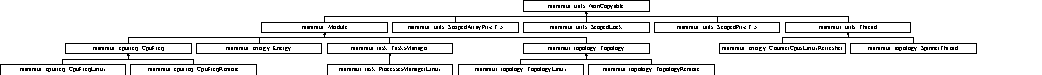
\includegraphics[height=1.014493cm]{classmammut_1_1utils_1_1NonCopyable}
\end{center}
\end{figure}


The documentation for this class was generated from the following file\-:\begin{DoxyCompactItemize}
\item 
/home/daniele/\-Code/\-Mammut/mammut/utils.\-hpp\end{DoxyCompactItemize}

\hypertarget{classmammut_1_1topology_1_1PhysicalCore}{\section{mammut\-:\-:topology\-:\-:Physical\-Core Class Reference}
\label{classmammut_1_1topology_1_1PhysicalCore}\index{mammut\-::topology\-::\-Physical\-Core@{mammut\-::topology\-::\-Physical\-Core}}
}
Inheritance diagram for mammut\-:\-:topology\-:\-:Physical\-Core\-:\begin{figure}[H]
\begin{center}
\leavevmode
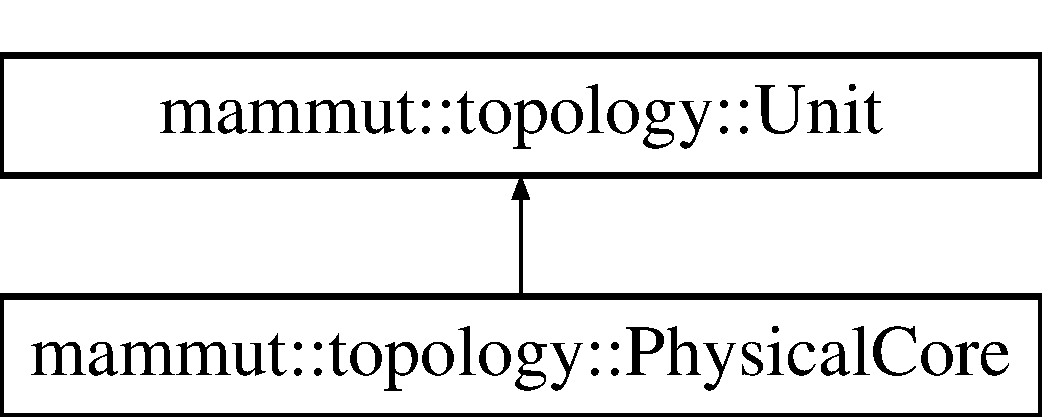
\includegraphics[height=3.000000cm]{classmammut_1_1topology_1_1PhysicalCore}
\end{center}
\end{figure}
\subsection*{Public Member Functions}
\begin{DoxyCompactItemize}
\item 
Physical\-Core\-Id \hyperlink{classmammut_1_1topology_1_1PhysicalCore_abbd39ff17b300c2ae85e97b6aaef9152}{get\-Physical\-Core\-Id} () const 
\item 
Cpu\-Id \hyperlink{classmammut_1_1topology_1_1PhysicalCore_a70bbe7bbdac1e9d55894b8360c151510}{get\-Cpu\-Id} () const 
\item 
std\-::vector$<$ \hyperlink{classmammut_1_1topology_1_1VirtualCore}{Virtual\-Core} $\ast$ $>$ \hyperlink{classmammut_1_1topology_1_1PhysicalCore_aca8047ed8a42413e67a20d52fefa824b}{get\-Virtual\-Cores} () const 
\item 
\hyperlink{classmammut_1_1topology_1_1VirtualCore}{Virtual\-Core} $\ast$ \hyperlink{classmammut_1_1topology_1_1PhysicalCore_afbf7299cc7f7ab7327c7419214f7de1a}{get\-Virtual\-Core} (Virtual\-Core\-Id virtual\-Core\-Id) const 
\item 
\hyperlink{classmammut_1_1topology_1_1VirtualCore}{Virtual\-Core} $\ast$ \hyperlink{classmammut_1_1topology_1_1PhysicalCore_ac35322afdb84c532fb82a53fcc7376f5}{get\-Virtual\-Core} () const 
\item 
virtual void \hyperlink{classmammut_1_1topology_1_1PhysicalCore_a2fe21bce321b3401e9108bcf29efafae}{maximize\-Utilization} () const =0
\item 
virtual void \hyperlink{classmammut_1_1topology_1_1PhysicalCore_ad6169b49eb4aa01fa570169735875ffe}{reset\-Utilization} () const =0
\end{DoxyCompactItemize}
\subsection*{Protected Member Functions}
\begin{DoxyCompactItemize}
\item 
\hypertarget{classmammut_1_1topology_1_1PhysicalCore_aaf7e5eb22971ccc42a2455484431c660}{{\bfseries Physical\-Core} (Cpu\-Id cpu\-Id, Physical\-Core\-Id physical\-Core\-Id, std\-::vector$<$ \hyperlink{classmammut_1_1topology_1_1VirtualCore}{Virtual\-Core} $\ast$ $>$ virtual\-Cores)}\label{classmammut_1_1topology_1_1PhysicalCore_aaf7e5eb22971ccc42a2455484431c660}

\end{DoxyCompactItemize}
\subsection*{Protected Attributes}
\begin{DoxyCompactItemize}
\item 
\hypertarget{classmammut_1_1topology_1_1PhysicalCore_a366e7d9045e2e0ce38c9a348856d41e6}{const Cpu\-Id {\bfseries \-\_\-cpu\-Id}}\label{classmammut_1_1topology_1_1PhysicalCore_a366e7d9045e2e0ce38c9a348856d41e6}

\item 
\hypertarget{classmammut_1_1topology_1_1PhysicalCore_ae1c83a9d2e61be31be246e9d0a2da0a0}{const Physical\-Core\-Id {\bfseries \-\_\-physical\-Core\-Id}}\label{classmammut_1_1topology_1_1PhysicalCore_ae1c83a9d2e61be31be246e9d0a2da0a0}

\item 
\hypertarget{classmammut_1_1topology_1_1PhysicalCore_a5d36d59b9bcc4e457a97d2797ce0c705}{const std\-::vector$<$ \hyperlink{classmammut_1_1topology_1_1VirtualCore}{Virtual\-Core} $\ast$ $>$ {\bfseries \-\_\-virtual\-Cores}}\label{classmammut_1_1topology_1_1PhysicalCore_a5d36d59b9bcc4e457a97d2797ce0c705}

\end{DoxyCompactItemize}


\subsection{Member Function Documentation}
\hypertarget{classmammut_1_1topology_1_1PhysicalCore_a70bbe7bbdac1e9d55894b8360c151510}{\index{mammut\-::topology\-::\-Physical\-Core@{mammut\-::topology\-::\-Physical\-Core}!get\-Cpu\-Id@{get\-Cpu\-Id}}
\index{get\-Cpu\-Id@{get\-Cpu\-Id}!mammut::topology::PhysicalCore@{mammut\-::topology\-::\-Physical\-Core}}
\subsubsection[{get\-Cpu\-Id}]{\setlength{\rightskip}{0pt plus 5cm}Cpu\-Id mammut\-::topology\-::\-Physical\-Core\-::get\-Cpu\-Id (
\begin{DoxyParamCaption}
{}
\end{DoxyParamCaption}
) const}}\label{classmammut_1_1topology_1_1PhysicalCore_a70bbe7bbdac1e9d55894b8360c151510}
Returns the identifier of the C\-P\-U where this physical core is running. \begin{DoxyReturn}{Returns}
The identifier of the C\-P\-U where this physical core is running. 
\end{DoxyReturn}
\hypertarget{classmammut_1_1topology_1_1PhysicalCore_abbd39ff17b300c2ae85e97b6aaef9152}{\index{mammut\-::topology\-::\-Physical\-Core@{mammut\-::topology\-::\-Physical\-Core}!get\-Physical\-Core\-Id@{get\-Physical\-Core\-Id}}
\index{get\-Physical\-Core\-Id@{get\-Physical\-Core\-Id}!mammut::topology::PhysicalCore@{mammut\-::topology\-::\-Physical\-Core}}
\subsubsection[{get\-Physical\-Core\-Id}]{\setlength{\rightskip}{0pt plus 5cm}Physical\-Core\-Id mammut\-::topology\-::\-Physical\-Core\-::get\-Physical\-Core\-Id (
\begin{DoxyParamCaption}
{}
\end{DoxyParamCaption}
) const}}\label{classmammut_1_1topology_1_1PhysicalCore_abbd39ff17b300c2ae85e97b6aaef9152}
Returns the identifier of this physical core.  The identifier of this physical core. \hypertarget{classmammut_1_1topology_1_1PhysicalCore_afbf7299cc7f7ab7327c7419214f7de1a}{\index{mammut\-::topology\-::\-Physical\-Core@{mammut\-::topology\-::\-Physical\-Core}!get\-Virtual\-Core@{get\-Virtual\-Core}}
\index{get\-Virtual\-Core@{get\-Virtual\-Core}!mammut::topology::PhysicalCore@{mammut\-::topology\-::\-Physical\-Core}}
\subsubsection[{get\-Virtual\-Core}]{\setlength{\rightskip}{0pt plus 5cm}{\bf Virtual\-Core} $\ast$ mammut\-::topology\-::\-Physical\-Core\-::get\-Virtual\-Core (
\begin{DoxyParamCaption}
\item[{Virtual\-Core\-Id}]{virtual\-Core\-Id}
\end{DoxyParamCaption}
) const}}\label{classmammut_1_1topology_1_1PhysicalCore_afbf7299cc7f7ab7327c7419214f7de1a}
Returns the virtual core with the given identifier, or N\-U\-L\-L if it is not present on this physical core. 
\begin{DoxyParams}{Parameters}
{\em virtual\-Core\-Id} & The identifier of the virtual core. \\
\hline
\end{DoxyParams}
\begin{DoxyReturn}{Returns}
The virtual core with the given identifier, or N\-U\-L\-L if it is not present on this physical core. 
\end{DoxyReturn}
\hypertarget{classmammut_1_1topology_1_1PhysicalCore_ac35322afdb84c532fb82a53fcc7376f5}{\index{mammut\-::topology\-::\-Physical\-Core@{mammut\-::topology\-::\-Physical\-Core}!get\-Virtual\-Core@{get\-Virtual\-Core}}
\index{get\-Virtual\-Core@{get\-Virtual\-Core}!mammut::topology::PhysicalCore@{mammut\-::topology\-::\-Physical\-Core}}
\subsubsection[{get\-Virtual\-Core}]{\setlength{\rightskip}{0pt plus 5cm}{\bf Virtual\-Core} $\ast$ mammut\-::topology\-::\-Physical\-Core\-::get\-Virtual\-Core (
\begin{DoxyParamCaption}
{}
\end{DoxyParamCaption}
) const}}\label{classmammut_1_1topology_1_1PhysicalCore_ac35322afdb84c532fb82a53fcc7376f5}
Returns a virtual core belonging to this physical core, or N\-U\-L\-L if it is not present. \begin{DoxyReturn}{Returns}
A virtual core belonging to this physical core, or N\-U\-L\-L if it is not present. 
\end{DoxyReturn}
\hypertarget{classmammut_1_1topology_1_1PhysicalCore_aca8047ed8a42413e67a20d52fefa824b}{\index{mammut\-::topology\-::\-Physical\-Core@{mammut\-::topology\-::\-Physical\-Core}!get\-Virtual\-Cores@{get\-Virtual\-Cores}}
\index{get\-Virtual\-Cores@{get\-Virtual\-Cores}!mammut::topology::PhysicalCore@{mammut\-::topology\-::\-Physical\-Core}}
\subsubsection[{get\-Virtual\-Cores}]{\setlength{\rightskip}{0pt plus 5cm}std\-::vector$<$ {\bf Virtual\-Core} $\ast$ $>$ mammut\-::topology\-::\-Physical\-Core\-::get\-Virtual\-Cores (
\begin{DoxyParamCaption}
{}
\end{DoxyParamCaption}
) const}}\label{classmammut_1_1topology_1_1PhysicalCore_aca8047ed8a42413e67a20d52fefa824b}
Returns the virtual cores associated to this physical core. \begin{DoxyReturn}{Returns}
The virtual cores associated to this physical core. 
\end{DoxyReturn}
\hypertarget{classmammut_1_1topology_1_1PhysicalCore_a2fe21bce321b3401e9108bcf29efafae}{\index{mammut\-::topology\-::\-Physical\-Core@{mammut\-::topology\-::\-Physical\-Core}!maximize\-Utilization@{maximize\-Utilization}}
\index{maximize\-Utilization@{maximize\-Utilization}!mammut::topology::PhysicalCore@{mammut\-::topology\-::\-Physical\-Core}}
\subsubsection[{maximize\-Utilization}]{\setlength{\rightskip}{0pt plus 5cm}virtual void mammut\-::topology\-::\-Physical\-Core\-::maximize\-Utilization (
\begin{DoxyParamCaption}
{}
\end{DoxyParamCaption}
) const\hspace{0.3cm}{\ttfamily [pure virtual]}}}\label{classmammut_1_1topology_1_1PhysicalCore_a2fe21bce321b3401e9108bcf29efafae}
Bring the utilization of this physical core to 100\% until \hyperlink{classmammut_1_1topology_1_1PhysicalCore_ad6169b49eb4aa01fa570169735875ffe}{reset\-Utilization()} is called. 

Implements \hyperlink{classmammut_1_1topology_1_1Unit_a0a12d2b5939c609c657a2bd652801e88}{mammut\-::topology\-::\-Unit}.



Implemented in \hyperlink{classmammut_1_1topology_1_1PhysicalCoreRemote_ad0207a63493483caedafd82faa354c40}{mammut\-::topology\-::\-Physical\-Core\-Remote}, and \hyperlink{classmammut_1_1topology_1_1PhysicalCoreLinux_a1f0d1fd02c9ac9a5960a880849affa45}{mammut\-::topology\-::\-Physical\-Core\-Linux}.

\hypertarget{classmammut_1_1topology_1_1PhysicalCore_ad6169b49eb4aa01fa570169735875ffe}{\index{mammut\-::topology\-::\-Physical\-Core@{mammut\-::topology\-::\-Physical\-Core}!reset\-Utilization@{reset\-Utilization}}
\index{reset\-Utilization@{reset\-Utilization}!mammut::topology::PhysicalCore@{mammut\-::topology\-::\-Physical\-Core}}
\subsubsection[{reset\-Utilization}]{\setlength{\rightskip}{0pt plus 5cm}virtual void mammut\-::topology\-::\-Physical\-Core\-::reset\-Utilization (
\begin{DoxyParamCaption}
{}
\end{DoxyParamCaption}
) const\hspace{0.3cm}{\ttfamily [pure virtual]}}}\label{classmammut_1_1topology_1_1PhysicalCore_ad6169b49eb4aa01fa570169735875ffe}
Resets the utilization of this physical core. 

Implements \hyperlink{classmammut_1_1topology_1_1Unit_a70730dde75533d3f5ecd3d3686df87cc}{mammut\-::topology\-::\-Unit}.



Implemented in \hyperlink{classmammut_1_1topology_1_1PhysicalCoreRemote_a5f76fa7a3b9c61597ad06a2fce8db675}{mammut\-::topology\-::\-Physical\-Core\-Remote}, and \hyperlink{classmammut_1_1topology_1_1PhysicalCoreLinux_a6c65161ad3041a8cedb8a9bc43757c02}{mammut\-::topology\-::\-Physical\-Core\-Linux}.



The documentation for this class was generated from the following files\-:\begin{DoxyCompactItemize}
\item 
/home/daniele/\-Code/\-Mammut/mammut/topology/topology.\-hpp\item 
/home/daniele/\-Code/\-Mammut/mammut/topology/topology.\-cpp\end{DoxyCompactItemize}

\hypertarget{classmammut_1_1topology_1_1PhysicalCoreLinux}{\section{mammut\-:\-:topology\-:\-:Physical\-Core\-Linux Class Reference}
\label{classmammut_1_1topology_1_1PhysicalCoreLinux}\index{mammut\-::topology\-::\-Physical\-Core\-Linux@{mammut\-::topology\-::\-Physical\-Core\-Linux}}
}
Inheritance diagram for mammut\-:\-:topology\-:\-:Physical\-Core\-Linux\-:\begin{figure}[H]
\begin{center}
\leavevmode
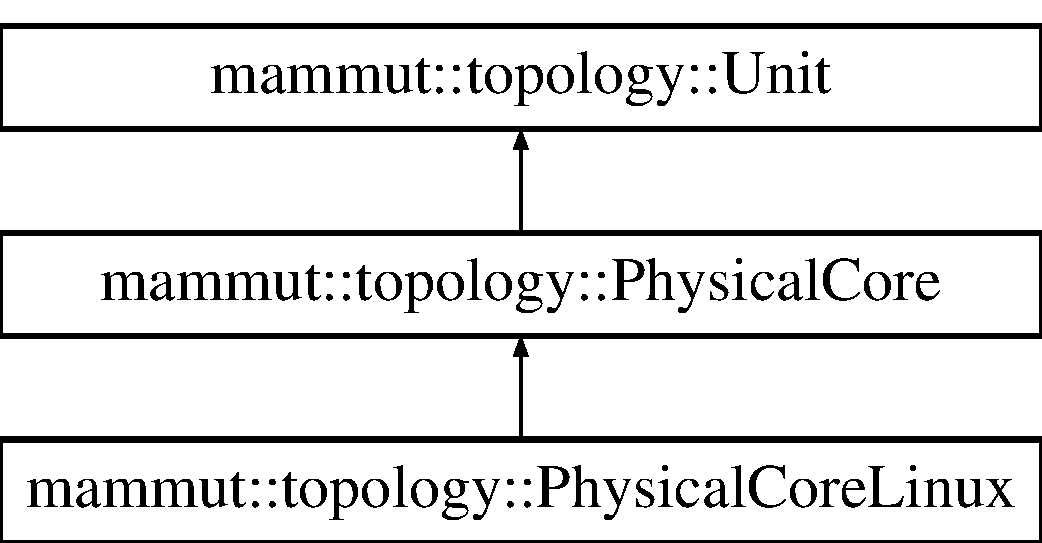
\includegraphics[height=3.000000cm]{classmammut_1_1topology_1_1PhysicalCoreLinux}
\end{center}
\end{figure}
\subsection*{Public Member Functions}
\begin{DoxyCompactItemize}
\item 
\hypertarget{classmammut_1_1topology_1_1PhysicalCoreLinux_a117187d74d105e7fb8cde0b58eed668b}{{\bfseries Physical\-Core\-Linux} (Cpu\-Id cpu\-Id, Physical\-Core\-Id physical\-Core\-Id, std\-::vector$<$ \hyperlink{classmammut_1_1topology_1_1VirtualCore}{Virtual\-Core} $\ast$ $>$ virtual\-Cores)}\label{classmammut_1_1topology_1_1PhysicalCoreLinux_a117187d74d105e7fb8cde0b58eed668b}

\item 
void \hyperlink{classmammut_1_1topology_1_1PhysicalCoreLinux_a1f0d1fd02c9ac9a5960a880849affa45}{maximize\-Utilization} () const 
\item 
void \hyperlink{classmammut_1_1topology_1_1PhysicalCoreLinux_a6c65161ad3041a8cedb8a9bc43757c02}{reset\-Utilization} () const 
\end{DoxyCompactItemize}
\subsection*{Additional Inherited Members}


\subsection{Member Function Documentation}
\hypertarget{classmammut_1_1topology_1_1PhysicalCoreLinux_a1f0d1fd02c9ac9a5960a880849affa45}{\index{mammut\-::topology\-::\-Physical\-Core\-Linux@{mammut\-::topology\-::\-Physical\-Core\-Linux}!maximize\-Utilization@{maximize\-Utilization}}
\index{maximize\-Utilization@{maximize\-Utilization}!mammut::topology::PhysicalCoreLinux@{mammut\-::topology\-::\-Physical\-Core\-Linux}}
\subsubsection[{maximize\-Utilization}]{\setlength{\rightskip}{0pt plus 5cm}void mammut\-::topology\-::\-Physical\-Core\-Linux\-::maximize\-Utilization (
\begin{DoxyParamCaption}
{}
\end{DoxyParamCaption}
) const\hspace{0.3cm}{\ttfamily [virtual]}}}\label{classmammut_1_1topology_1_1PhysicalCoreLinux_a1f0d1fd02c9ac9a5960a880849affa45}
Bring the utilization of this physical core to 100\% until \hyperlink{classmammut_1_1topology_1_1PhysicalCoreLinux_a6c65161ad3041a8cedb8a9bc43757c02}{reset\-Utilization()} is called. 

Implements \hyperlink{classmammut_1_1topology_1_1PhysicalCore_a2fe21bce321b3401e9108bcf29efafae}{mammut\-::topology\-::\-Physical\-Core}.

\hypertarget{classmammut_1_1topology_1_1PhysicalCoreLinux_a6c65161ad3041a8cedb8a9bc43757c02}{\index{mammut\-::topology\-::\-Physical\-Core\-Linux@{mammut\-::topology\-::\-Physical\-Core\-Linux}!reset\-Utilization@{reset\-Utilization}}
\index{reset\-Utilization@{reset\-Utilization}!mammut::topology::PhysicalCoreLinux@{mammut\-::topology\-::\-Physical\-Core\-Linux}}
\subsubsection[{reset\-Utilization}]{\setlength{\rightskip}{0pt plus 5cm}void mammut\-::topology\-::\-Physical\-Core\-Linux\-::reset\-Utilization (
\begin{DoxyParamCaption}
{}
\end{DoxyParamCaption}
) const\hspace{0.3cm}{\ttfamily [virtual]}}}\label{classmammut_1_1topology_1_1PhysicalCoreLinux_a6c65161ad3041a8cedb8a9bc43757c02}
Resets the utilization of this physical core. 

Implements \hyperlink{classmammut_1_1topology_1_1PhysicalCore_ad6169b49eb4aa01fa570169735875ffe}{mammut\-::topology\-::\-Physical\-Core}.



The documentation for this class was generated from the following files\-:\begin{DoxyCompactItemize}
\item 
/home/daniele/\-Code/\-Mammut/mammut/topology/topology-\/linux.\-hpp\item 
/home/daniele/\-Code/\-Mammut/mammut/topology/topology-\/linux.\-cpp\end{DoxyCompactItemize}

\hypertarget{classmammut_1_1topology_1_1PhysicalCoreRemote}{\section{mammut\-:\-:topology\-:\-:Physical\-Core\-Remote Class Reference}
\label{classmammut_1_1topology_1_1PhysicalCoreRemote}\index{mammut\-::topology\-::\-Physical\-Core\-Remote@{mammut\-::topology\-::\-Physical\-Core\-Remote}}
}
Inheritance diagram for mammut\-:\-:topology\-:\-:Physical\-Core\-Remote\-:\begin{figure}[H]
\begin{center}
\leavevmode
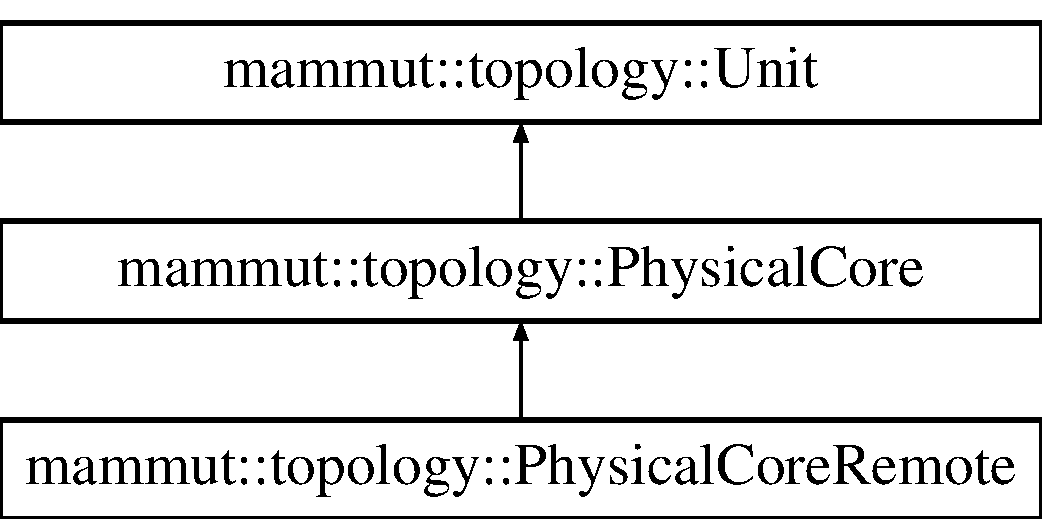
\includegraphics[height=3.000000cm]{classmammut_1_1topology_1_1PhysicalCoreRemote}
\end{center}
\end{figure}
\subsection*{Public Member Functions}
\begin{DoxyCompactItemize}
\item 
\hypertarget{classmammut_1_1topology_1_1PhysicalCoreRemote_a87e4c8dda013d6501584f2feda4e0a06}{{\bfseries Physical\-Core\-Remote} (\hyperlink{classmammut_1_1Communicator}{Communicator} $\ast$const communicator, Cpu\-Id cpu\-Id, Physical\-Core\-Id physical\-Core\-Id, std\-::vector$<$ \hyperlink{classmammut_1_1topology_1_1VirtualCore}{Virtual\-Core} $\ast$ $>$ virtual\-Cores)}\label{classmammut_1_1topology_1_1PhysicalCoreRemote_a87e4c8dda013d6501584f2feda4e0a06}

\item 
void \hyperlink{classmammut_1_1topology_1_1PhysicalCoreRemote_ad0207a63493483caedafd82faa354c40}{maximize\-Utilization} () const 
\item 
void \hyperlink{classmammut_1_1topology_1_1PhysicalCoreRemote_a5f76fa7a3b9c61597ad06a2fce8db675}{reset\-Utilization} () const 
\end{DoxyCompactItemize}
\subsection*{Additional Inherited Members}


\subsection{Member Function Documentation}
\hypertarget{classmammut_1_1topology_1_1PhysicalCoreRemote_ad0207a63493483caedafd82faa354c40}{\index{mammut\-::topology\-::\-Physical\-Core\-Remote@{mammut\-::topology\-::\-Physical\-Core\-Remote}!maximize\-Utilization@{maximize\-Utilization}}
\index{maximize\-Utilization@{maximize\-Utilization}!mammut::topology::PhysicalCoreRemote@{mammut\-::topology\-::\-Physical\-Core\-Remote}}
\subsubsection[{maximize\-Utilization}]{\setlength{\rightskip}{0pt plus 5cm}void mammut\-::topology\-::\-Physical\-Core\-Remote\-::maximize\-Utilization (
\begin{DoxyParamCaption}
{}
\end{DoxyParamCaption}
) const\hspace{0.3cm}{\ttfamily [virtual]}}}\label{classmammut_1_1topology_1_1PhysicalCoreRemote_ad0207a63493483caedafd82faa354c40}
Bring the utilization of this physical core to 100\% until \hyperlink{classmammut_1_1topology_1_1PhysicalCoreRemote_a5f76fa7a3b9c61597ad06a2fce8db675}{reset\-Utilization()} is called. 

Implements \hyperlink{classmammut_1_1topology_1_1PhysicalCore_a2fe21bce321b3401e9108bcf29efafae}{mammut\-::topology\-::\-Physical\-Core}.

\hypertarget{classmammut_1_1topology_1_1PhysicalCoreRemote_a5f76fa7a3b9c61597ad06a2fce8db675}{\index{mammut\-::topology\-::\-Physical\-Core\-Remote@{mammut\-::topology\-::\-Physical\-Core\-Remote}!reset\-Utilization@{reset\-Utilization}}
\index{reset\-Utilization@{reset\-Utilization}!mammut::topology::PhysicalCoreRemote@{mammut\-::topology\-::\-Physical\-Core\-Remote}}
\subsubsection[{reset\-Utilization}]{\setlength{\rightskip}{0pt plus 5cm}void mammut\-::topology\-::\-Physical\-Core\-Remote\-::reset\-Utilization (
\begin{DoxyParamCaption}
{}
\end{DoxyParamCaption}
) const\hspace{0.3cm}{\ttfamily [virtual]}}}\label{classmammut_1_1topology_1_1PhysicalCoreRemote_a5f76fa7a3b9c61597ad06a2fce8db675}
Resets the utilization of this physical core. 

Implements \hyperlink{classmammut_1_1topology_1_1PhysicalCore_ad6169b49eb4aa01fa570169735875ffe}{mammut\-::topology\-::\-Physical\-Core}.



The documentation for this class was generated from the following file\-:\begin{DoxyCompactItemize}
\item 
/home/daniele/\-Code/\-Mammut/mammut/topology/topology-\/remote.\-hpp\end{DoxyCompactItemize}

\hypertarget{classmammut_1_1task_1_1ProcessesManagerLinux}{\section{mammut\-:\-:task\-:\-:Processes\-Manager\-Linux Class Reference}
\label{classmammut_1_1task_1_1ProcessesManagerLinux}\index{mammut\-::task\-::\-Processes\-Manager\-Linux@{mammut\-::task\-::\-Processes\-Manager\-Linux}}
}
Inheritance diagram for mammut\-:\-:task\-:\-:Processes\-Manager\-Linux\-:\begin{figure}[H]
\begin{center}
\leavevmode
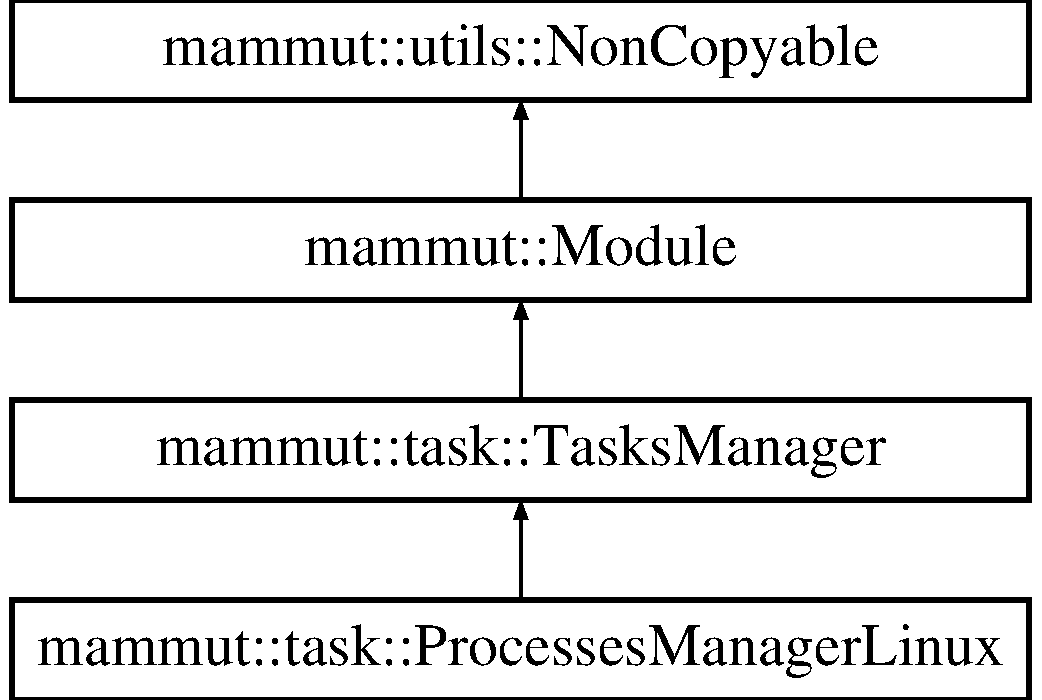
\includegraphics[height=4.000000cm]{classmammut_1_1task_1_1ProcessesManagerLinux}
\end{center}
\end{figure}
\subsection*{Public Member Functions}
\begin{DoxyCompactItemize}
\item 
std\-::vector$<$ Task\-Id $>$ \hyperlink{classmammut_1_1task_1_1ProcessesManagerLinux_a462f03471eb2d33aa9c9b356d2cffe59}{get\-Active\-Processes\-Identifiers} () const 
\item 
\hyperlink{classmammut_1_1task_1_1ProcessHandler}{Process\-Handler} $\ast$ \hyperlink{classmammut_1_1task_1_1ProcessesManagerLinux_a3d2102056565bb09e0c15e352a741451}{get\-Process\-Handler} (Task\-Id pid) const 
\item 
void \hyperlink{classmammut_1_1task_1_1ProcessesManagerLinux_afef064167534e4108e6ca33277bbbbb7}{release\-Process\-Handler} (\hyperlink{classmammut_1_1task_1_1ProcessHandler}{Process\-Handler} $\ast$process) const 
\item 
\hyperlink{classmammut_1_1task_1_1ThreadHandler}{Thread\-Handler} $\ast$ \hyperlink{classmammut_1_1task_1_1ProcessesManagerLinux_ad3d15ed36d4deca35e2dd88d304fa301}{get\-Thread\-Handler} (Task\-Id pid, Task\-Id tid) const 
\item 
\hyperlink{classmammut_1_1task_1_1ThreadHandler}{Thread\-Handler} $\ast$ \hyperlink{classmammut_1_1task_1_1ProcessesManagerLinux_ab52208db53ef4ddb0a8b9661ef6b255a}{get\-Thread\-Handler} () const 
\item 
void \hyperlink{classmammut_1_1task_1_1ProcessesManagerLinux_ad9d72966c952c4d2dd1445204d600667}{release\-Thread\-Handler} (\hyperlink{classmammut_1_1task_1_1ThreadHandler}{Thread\-Handler} $\ast$thread) const 
\end{DoxyCompactItemize}


\subsection{Member Function Documentation}
\hypertarget{classmammut_1_1task_1_1ProcessesManagerLinux_a462f03471eb2d33aa9c9b356d2cffe59}{\index{mammut\-::task\-::\-Processes\-Manager\-Linux@{mammut\-::task\-::\-Processes\-Manager\-Linux}!get\-Active\-Processes\-Identifiers@{get\-Active\-Processes\-Identifiers}}
\index{get\-Active\-Processes\-Identifiers@{get\-Active\-Processes\-Identifiers}!mammut::task::ProcessesManagerLinux@{mammut\-::task\-::\-Processes\-Manager\-Linux}}
\subsubsection[{get\-Active\-Processes\-Identifiers}]{\setlength{\rightskip}{0pt plus 5cm}std\-::vector$<$ Task\-Id $>$ mammut\-::task\-::\-Processes\-Manager\-Linux\-::get\-Active\-Processes\-Identifiers (
\begin{DoxyParamCaption}
{}
\end{DoxyParamCaption}
) const\hspace{0.3cm}{\ttfamily [virtual]}}}\label{classmammut_1_1task_1_1ProcessesManagerLinux_a462f03471eb2d33aa9c9b356d2cffe59}
Returns a list of active processes identifiers. \begin{DoxyReturn}{Returns}
A vector of active processes identifiers. 
\end{DoxyReturn}


Implements \hyperlink{classmammut_1_1task_1_1TasksManager_a301de447218cce0ae1f81af943ea6fe5}{mammut\-::task\-::\-Tasks\-Manager}.

\hypertarget{classmammut_1_1task_1_1ProcessesManagerLinux_a3d2102056565bb09e0c15e352a741451}{\index{mammut\-::task\-::\-Processes\-Manager\-Linux@{mammut\-::task\-::\-Processes\-Manager\-Linux}!get\-Process\-Handler@{get\-Process\-Handler}}
\index{get\-Process\-Handler@{get\-Process\-Handler}!mammut::task::ProcessesManagerLinux@{mammut\-::task\-::\-Processes\-Manager\-Linux}}
\subsubsection[{get\-Process\-Handler}]{\setlength{\rightskip}{0pt plus 5cm}{\bf Process\-Handler} $\ast$ mammut\-::task\-::\-Processes\-Manager\-Linux\-::get\-Process\-Handler (
\begin{DoxyParamCaption}
\item[{Task\-Id}]{pid}
\end{DoxyParamCaption}
) const\hspace{0.3cm}{\ttfamily [virtual]}}}\label{classmammut_1_1task_1_1ProcessesManagerLinux_a3d2102056565bb09e0c15e352a741451}
Returns the handler associated to a specific process. 
\begin{DoxyParams}{Parameters}
{\em pid} & The process identifier. \\
\hline
\end{DoxyParams}
\begin{DoxyReturn}{Returns}
The handler associated to a specific process or N\-U\-L\-L if the process doesn't exists. The obtained handler must be released with release\-Process\-Handler call. 
\end{DoxyReturn}


Implements \hyperlink{classmammut_1_1task_1_1TasksManager_a529f75258ad54951209786ebfec1d658}{mammut\-::task\-::\-Tasks\-Manager}.

\hypertarget{classmammut_1_1task_1_1ProcessesManagerLinux_ad3d15ed36d4deca35e2dd88d304fa301}{\index{mammut\-::task\-::\-Processes\-Manager\-Linux@{mammut\-::task\-::\-Processes\-Manager\-Linux}!get\-Thread\-Handler@{get\-Thread\-Handler}}
\index{get\-Thread\-Handler@{get\-Thread\-Handler}!mammut::task::ProcessesManagerLinux@{mammut\-::task\-::\-Processes\-Manager\-Linux}}
\subsubsection[{get\-Thread\-Handler}]{\setlength{\rightskip}{0pt plus 5cm}{\bf Thread\-Handler} $\ast$ mammut\-::task\-::\-Processes\-Manager\-Linux\-::get\-Thread\-Handler (
\begin{DoxyParamCaption}
\item[{Task\-Id}]{pid, }
\item[{Task\-Id}]{tid}
\end{DoxyParamCaption}
) const\hspace{0.3cm}{\ttfamily [virtual]}}}\label{classmammut_1_1task_1_1ProcessesManagerLinux_ad3d15ed36d4deca35e2dd88d304fa301}
Returns the handler associated to a specific thread. 
\begin{DoxyParams}{Parameters}
{\em pid} & The process identifier. \\
\hline
{\em tid} & The thread identifier. \\
\hline
\end{DoxyParams}
\begin{DoxyReturn}{Returns}
The handler associated to a specific thread or N\-U\-L\-L if the thread doesn't exists. The obtained handler must be released with release\-Thread\-Handler call. 
\end{DoxyReturn}


Implements \hyperlink{classmammut_1_1task_1_1TasksManager_a3c4a48df7d66c4fcf56c055d951d6bbe}{mammut\-::task\-::\-Tasks\-Manager}.

\hypertarget{classmammut_1_1task_1_1ProcessesManagerLinux_ab52208db53ef4ddb0a8b9661ef6b255a}{\index{mammut\-::task\-::\-Processes\-Manager\-Linux@{mammut\-::task\-::\-Processes\-Manager\-Linux}!get\-Thread\-Handler@{get\-Thread\-Handler}}
\index{get\-Thread\-Handler@{get\-Thread\-Handler}!mammut::task::ProcessesManagerLinux@{mammut\-::task\-::\-Processes\-Manager\-Linux}}
\subsubsection[{get\-Thread\-Handler}]{\setlength{\rightskip}{0pt plus 5cm}{\bf Thread\-Handler} $\ast$ mammut\-::task\-::\-Processes\-Manager\-Linux\-::get\-Thread\-Handler (
\begin{DoxyParamCaption}
{}
\end{DoxyParamCaption}
) const\hspace{0.3cm}{\ttfamily [virtual]}}}\label{classmammut_1_1task_1_1ProcessesManagerLinux_ab52208db53ef4ddb0a8b9661ef6b255a}
Returns the handler associated to the calling thread. \begin{DoxyReturn}{Returns}
The handler associated to the calling thread. The obtained handler must be released with release\-Thread\-Handler call. 
\end{DoxyReturn}


Implements \hyperlink{classmammut_1_1task_1_1TasksManager_abf218ec9437ec3b6e2257715063b7262}{mammut\-::task\-::\-Tasks\-Manager}.

\hypertarget{classmammut_1_1task_1_1ProcessesManagerLinux_afef064167534e4108e6ca33277bbbbb7}{\index{mammut\-::task\-::\-Processes\-Manager\-Linux@{mammut\-::task\-::\-Processes\-Manager\-Linux}!release\-Process\-Handler@{release\-Process\-Handler}}
\index{release\-Process\-Handler@{release\-Process\-Handler}!mammut::task::ProcessesManagerLinux@{mammut\-::task\-::\-Processes\-Manager\-Linux}}
\subsubsection[{release\-Process\-Handler}]{\setlength{\rightskip}{0pt plus 5cm}void mammut\-::task\-::\-Processes\-Manager\-Linux\-::release\-Process\-Handler (
\begin{DoxyParamCaption}
\item[{{\bf Process\-Handler} $\ast$}]{process}
\end{DoxyParamCaption}
) const\hspace{0.3cm}{\ttfamily [virtual]}}}\label{classmammut_1_1task_1_1ProcessesManagerLinux_afef064167534e4108e6ca33277bbbbb7}
Releases the handler obtained through get\-Process\-Handler call. 
\begin{DoxyParams}{Parameters}
{\em process} & The process handler. \\
\hline
\end{DoxyParams}


Implements \hyperlink{classmammut_1_1task_1_1TasksManager_ad97b2200f285f63f6e8858cce31422d3}{mammut\-::task\-::\-Tasks\-Manager}.

\hypertarget{classmammut_1_1task_1_1ProcessesManagerLinux_ad9d72966c952c4d2dd1445204d600667}{\index{mammut\-::task\-::\-Processes\-Manager\-Linux@{mammut\-::task\-::\-Processes\-Manager\-Linux}!release\-Thread\-Handler@{release\-Thread\-Handler}}
\index{release\-Thread\-Handler@{release\-Thread\-Handler}!mammut::task::ProcessesManagerLinux@{mammut\-::task\-::\-Processes\-Manager\-Linux}}
\subsubsection[{release\-Thread\-Handler}]{\setlength{\rightskip}{0pt plus 5cm}void mammut\-::task\-::\-Processes\-Manager\-Linux\-::release\-Thread\-Handler (
\begin{DoxyParamCaption}
\item[{{\bf Thread\-Handler} $\ast$}]{thread}
\end{DoxyParamCaption}
) const\hspace{0.3cm}{\ttfamily [virtual]}}}\label{classmammut_1_1task_1_1ProcessesManagerLinux_ad9d72966c952c4d2dd1445204d600667}
Releases the handler obtained through get\-Thread\-Handler call. 
\begin{DoxyParams}{Parameters}
{\em thread} & The thread handler. \\
\hline
\end{DoxyParams}


Implements \hyperlink{classmammut_1_1task_1_1TasksManager_af5ad5db5b43441a49e0a5633dd1ff667}{mammut\-::task\-::\-Tasks\-Manager}.



The documentation for this class was generated from the following files\-:\begin{DoxyCompactItemize}
\item 
/home/daniele/\-Code/\-Mammut/mammut/task/task-\/linux.\-hpp\item 
/home/daniele/\-Code/\-Mammut/mammut/task/task-\/linux.\-cpp\end{DoxyCompactItemize}

\hypertarget{classmammut_1_1task_1_1ProcessHandler}{\section{mammut\-:\-:task\-:\-:Process\-Handler Class Reference}
\label{classmammut_1_1task_1_1ProcessHandler}\index{mammut\-::task\-::\-Process\-Handler@{mammut\-::task\-::\-Process\-Handler}}
}
Inheritance diagram for mammut\-:\-:task\-:\-:Process\-Handler\-:\begin{figure}[H]
\begin{center}
\leavevmode
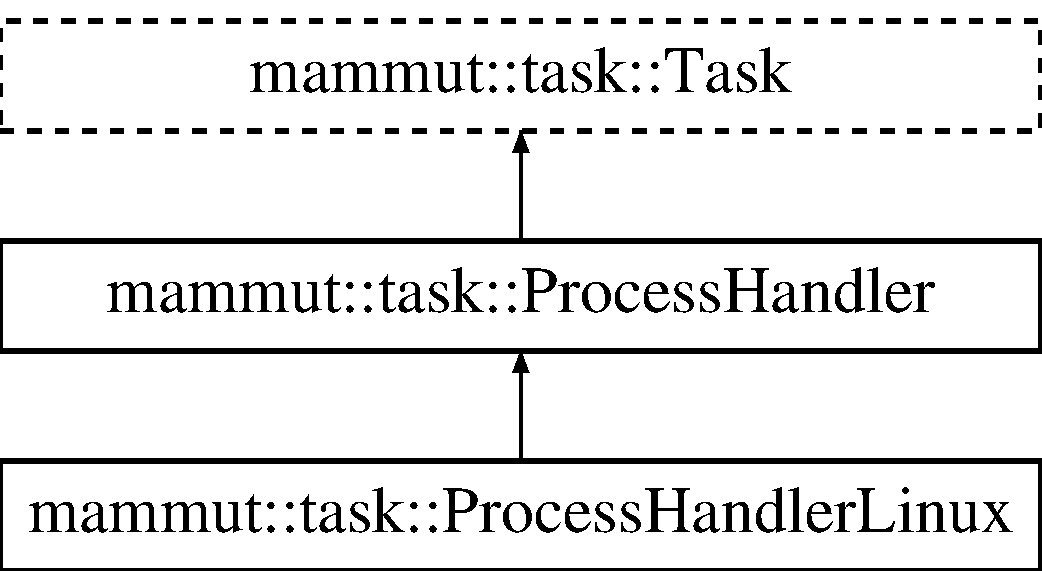
\includegraphics[height=3.000000cm]{classmammut_1_1task_1_1ProcessHandler}
\end{center}
\end{figure}
\subsection*{Public Member Functions}
\begin{DoxyCompactItemize}
\item 
virtual std\-::vector$<$ Task\-Id $>$ \hyperlink{classmammut_1_1task_1_1ProcessHandler_a210393636fbfa4658e80978b2c0d8556}{get\-Active\-Threads\-Identifiers} () const =0
\item 
virtual \hyperlink{classmammut_1_1task_1_1ThreadHandler}{Thread\-Handler} $\ast$ \hyperlink{classmammut_1_1task_1_1ProcessHandler_acdf10305751075accee3fb846469a2f6}{get\-Thread\-Handler} (Task\-Id tid) const =0
\item 
virtual void \hyperlink{classmammut_1_1task_1_1ProcessHandler_aad1791569e9f48ef5559ceeb897e7a1a}{release\-Thread\-Handler} (\hyperlink{classmammut_1_1task_1_1ThreadHandler}{Thread\-Handler} $\ast$thread) const =0
\end{DoxyCompactItemize}


\subsection{Member Function Documentation}
\hypertarget{classmammut_1_1task_1_1ProcessHandler_a210393636fbfa4658e80978b2c0d8556}{\index{mammut\-::task\-::\-Process\-Handler@{mammut\-::task\-::\-Process\-Handler}!get\-Active\-Threads\-Identifiers@{get\-Active\-Threads\-Identifiers}}
\index{get\-Active\-Threads\-Identifiers@{get\-Active\-Threads\-Identifiers}!mammut::task::ProcessHandler@{mammut\-::task\-::\-Process\-Handler}}
\subsubsection[{get\-Active\-Threads\-Identifiers}]{\setlength{\rightskip}{0pt plus 5cm}virtual std\-::vector$<$Task\-Id$>$ mammut\-::task\-::\-Process\-Handler\-::get\-Active\-Threads\-Identifiers (
\begin{DoxyParamCaption}
{}
\end{DoxyParamCaption}
) const\hspace{0.3cm}{\ttfamily [pure virtual]}}}\label{classmammut_1_1task_1_1ProcessHandler_a210393636fbfa4658e80978b2c0d8556}
Returns a list of active thread identifiers on this process. \begin{DoxyReturn}{Returns}
A vector of active thread identifiers on this process. 
\end{DoxyReturn}


Implemented in \hyperlink{classmammut_1_1task_1_1ProcessHandlerLinux_a6d0d7380036a11cedec33f8e15216d2b}{mammut\-::task\-::\-Process\-Handler\-Linux}.

\hypertarget{classmammut_1_1task_1_1ProcessHandler_acdf10305751075accee3fb846469a2f6}{\index{mammut\-::task\-::\-Process\-Handler@{mammut\-::task\-::\-Process\-Handler}!get\-Thread\-Handler@{get\-Thread\-Handler}}
\index{get\-Thread\-Handler@{get\-Thread\-Handler}!mammut::task::ProcessHandler@{mammut\-::task\-::\-Process\-Handler}}
\subsubsection[{get\-Thread\-Handler}]{\setlength{\rightskip}{0pt plus 5cm}virtual {\bf Thread\-Handler}$\ast$ mammut\-::task\-::\-Process\-Handler\-::get\-Thread\-Handler (
\begin{DoxyParamCaption}
\item[{Task\-Id}]{tid}
\end{DoxyParamCaption}
) const\hspace{0.3cm}{\ttfamily [pure virtual]}}}\label{classmammut_1_1task_1_1ProcessHandler_acdf10305751075accee3fb846469a2f6}
Returns the handler associated to a specific thread. 
\begin{DoxyParams}{Parameters}
{\em tid} & The thread identifier. \\
\hline
\end{DoxyParams}
\begin{DoxyReturn}{Returns}
The handler associated to a specific thread or N\-U\-L\-L if the thread doesn't exists. The obtained handler must be released with release\-Thread\-Handler call. 
\end{DoxyReturn}


Implemented in \hyperlink{classmammut_1_1task_1_1ProcessHandlerLinux_a5cc938433da546d816a1318af40abc82}{mammut\-::task\-::\-Process\-Handler\-Linux}.

\hypertarget{classmammut_1_1task_1_1ProcessHandler_aad1791569e9f48ef5559ceeb897e7a1a}{\index{mammut\-::task\-::\-Process\-Handler@{mammut\-::task\-::\-Process\-Handler}!release\-Thread\-Handler@{release\-Thread\-Handler}}
\index{release\-Thread\-Handler@{release\-Thread\-Handler}!mammut::task::ProcessHandler@{mammut\-::task\-::\-Process\-Handler}}
\subsubsection[{release\-Thread\-Handler}]{\setlength{\rightskip}{0pt plus 5cm}virtual void mammut\-::task\-::\-Process\-Handler\-::release\-Thread\-Handler (
\begin{DoxyParamCaption}
\item[{{\bf Thread\-Handler} $\ast$}]{thread}
\end{DoxyParamCaption}
) const\hspace{0.3cm}{\ttfamily [pure virtual]}}}\label{classmammut_1_1task_1_1ProcessHandler_aad1791569e9f48ef5559ceeb897e7a1a}
Releases the handler obtained through get\-Thread\-Handler call. 
\begin{DoxyParams}{Parameters}
{\em thread} & The thread handler. \\
\hline
\end{DoxyParams}


Implemented in \hyperlink{classmammut_1_1task_1_1ProcessHandlerLinux_abf3faf0d2aa1d28b1efd51c4759570be}{mammut\-::task\-::\-Process\-Handler\-Linux}.



The documentation for this class was generated from the following file\-:\begin{DoxyCompactItemize}
\item 
/home/daniele/\-Code/\-Mammut/mammut/task/task.\-hpp\end{DoxyCompactItemize}

\hypertarget{classmammut_1_1task_1_1ProcessHandlerLinux}{\section{mammut\-:\-:task\-:\-:Process\-Handler\-Linux Class Reference}
\label{classmammut_1_1task_1_1ProcessHandlerLinux}\index{mammut\-::task\-::\-Process\-Handler\-Linux@{mammut\-::task\-::\-Process\-Handler\-Linux}}
}
Inheritance diagram for mammut\-:\-:task\-:\-:Process\-Handler\-Linux\-:\begin{figure}[H]
\begin{center}
\leavevmode
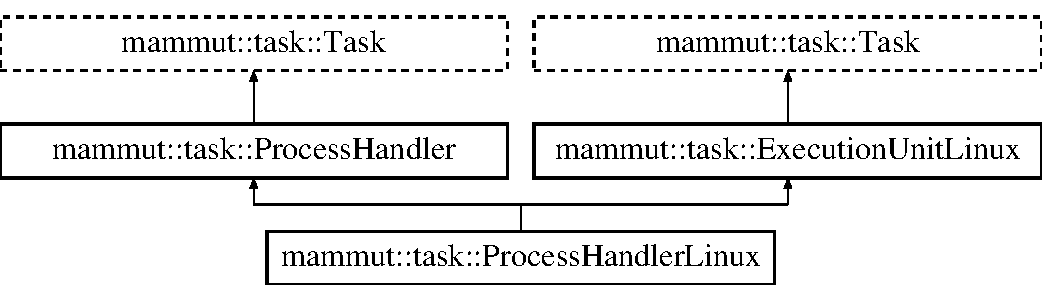
\includegraphics[height=3.000000cm]{classmammut_1_1task_1_1ProcessHandlerLinux}
\end{center}
\end{figure}
\subsection*{Public Member Functions}
\begin{DoxyCompactItemize}
\item 
\hypertarget{classmammut_1_1task_1_1ProcessHandlerLinux_abc9e76a8d43797d06839f29ec4b5f750}{{\bfseries Process\-Handler\-Linux} (Task\-Id pid)}\label{classmammut_1_1task_1_1ProcessHandlerLinux_abc9e76a8d43797d06839f29ec4b5f750}

\item 
std\-::vector$<$ Task\-Id $>$ \hyperlink{classmammut_1_1task_1_1ProcessHandlerLinux_a6d0d7380036a11cedec33f8e15216d2b}{get\-Active\-Threads\-Identifiers} () const 
\item 
\hyperlink{classmammut_1_1task_1_1ThreadHandler}{Thread\-Handler} $\ast$ \hyperlink{classmammut_1_1task_1_1ProcessHandlerLinux_a5cc938433da546d816a1318af40abc82}{get\-Thread\-Handler} (Task\-Id tid) const 
\item 
void \hyperlink{classmammut_1_1task_1_1ProcessHandlerLinux_abf3faf0d2aa1d28b1efd51c4759570be}{release\-Thread\-Handler} (\hyperlink{classmammut_1_1task_1_1ThreadHandler}{Thread\-Handler} $\ast$thread) const 
\item 
bool \hyperlink{classmammut_1_1task_1_1ProcessHandlerLinux_afe9e66ee6d87efd57c9bbfcc51ec0db6}{move} (const std\-::vector$<$ topology\-::\-Virtual\-Core\-Id $>$ virtual\-Cores\-Ids) const 
\end{DoxyCompactItemize}


\subsection{Member Function Documentation}
\hypertarget{classmammut_1_1task_1_1ProcessHandlerLinux_a6d0d7380036a11cedec33f8e15216d2b}{\index{mammut\-::task\-::\-Process\-Handler\-Linux@{mammut\-::task\-::\-Process\-Handler\-Linux}!get\-Active\-Threads\-Identifiers@{get\-Active\-Threads\-Identifiers}}
\index{get\-Active\-Threads\-Identifiers@{get\-Active\-Threads\-Identifiers}!mammut::task::ProcessHandlerLinux@{mammut\-::task\-::\-Process\-Handler\-Linux}}
\subsubsection[{get\-Active\-Threads\-Identifiers}]{\setlength{\rightskip}{0pt plus 5cm}std\-::vector$<$ Task\-Id $>$ mammut\-::task\-::\-Process\-Handler\-Linux\-::get\-Active\-Threads\-Identifiers (
\begin{DoxyParamCaption}
{}
\end{DoxyParamCaption}
) const\hspace{0.3cm}{\ttfamily [virtual]}}}\label{classmammut_1_1task_1_1ProcessHandlerLinux_a6d0d7380036a11cedec33f8e15216d2b}
Returns a list of active thread identifiers on this process. \begin{DoxyReturn}{Returns}
A vector of active thread identifiers on this process. 
\end{DoxyReturn}


Implements \hyperlink{classmammut_1_1task_1_1ProcessHandler_a210393636fbfa4658e80978b2c0d8556}{mammut\-::task\-::\-Process\-Handler}.

\hypertarget{classmammut_1_1task_1_1ProcessHandlerLinux_a5cc938433da546d816a1318af40abc82}{\index{mammut\-::task\-::\-Process\-Handler\-Linux@{mammut\-::task\-::\-Process\-Handler\-Linux}!get\-Thread\-Handler@{get\-Thread\-Handler}}
\index{get\-Thread\-Handler@{get\-Thread\-Handler}!mammut::task::ProcessHandlerLinux@{mammut\-::task\-::\-Process\-Handler\-Linux}}
\subsubsection[{get\-Thread\-Handler}]{\setlength{\rightskip}{0pt plus 5cm}{\bf Thread\-Handler} $\ast$ mammut\-::task\-::\-Process\-Handler\-Linux\-::get\-Thread\-Handler (
\begin{DoxyParamCaption}
\item[{Task\-Id}]{tid}
\end{DoxyParamCaption}
) const\hspace{0.3cm}{\ttfamily [virtual]}}}\label{classmammut_1_1task_1_1ProcessHandlerLinux_a5cc938433da546d816a1318af40abc82}
Returns the handler associated to a specific thread. 
\begin{DoxyParams}{Parameters}
{\em tid} & The thread identifier. \\
\hline
\end{DoxyParams}
\begin{DoxyReturn}{Returns}
The handler associated to a specific thread or N\-U\-L\-L if the thread doesn't exists. The obtained handler must be released with release\-Thread\-Handler call. 
\end{DoxyReturn}


Implements \hyperlink{classmammut_1_1task_1_1ProcessHandler_acdf10305751075accee3fb846469a2f6}{mammut\-::task\-::\-Process\-Handler}.

\hypertarget{classmammut_1_1task_1_1ProcessHandlerLinux_afe9e66ee6d87efd57c9bbfcc51ec0db6}{\index{mammut\-::task\-::\-Process\-Handler\-Linux@{mammut\-::task\-::\-Process\-Handler\-Linux}!move@{move}}
\index{move@{move}!mammut::task::ProcessHandlerLinux@{mammut\-::task\-::\-Process\-Handler\-Linux}}
\subsubsection[{move}]{\setlength{\rightskip}{0pt plus 5cm}bool mammut\-::task\-::\-Process\-Handler\-Linux\-::move (
\begin{DoxyParamCaption}
\item[{const std\-::vector$<$ topology\-::\-Virtual\-Core\-Id $>$}]{virtual\-Cores\-Ids}
\end{DoxyParamCaption}
) const\hspace{0.3cm}{\ttfamily [virtual]}}}\label{classmammut_1_1task_1_1ProcessHandlerLinux_afe9e66ee6d87efd57c9bbfcc51ec0db6}
Move this execution unit on a set of specified virtual cores. 
\begin{DoxyParams}{Parameters}
{\em virtual\-Cores\-Ids} & The identifiers of the virtual cores on which this execution unit must be moved. \\
\hline
\end{DoxyParams}
\begin{DoxyReturn}{Returns}
If false is returned, this execution unit is no more active and the call failed. Otherwise, true is returned. 
\end{DoxyReturn}


Implements \hyperlink{classmammut_1_1task_1_1ExecutionUnitLinux_aedac673e0c581fcbfc6b3fb5a38cd81b}{mammut\-::task\-::\-Execution\-Unit\-Linux}.

\hypertarget{classmammut_1_1task_1_1ProcessHandlerLinux_abf3faf0d2aa1d28b1efd51c4759570be}{\index{mammut\-::task\-::\-Process\-Handler\-Linux@{mammut\-::task\-::\-Process\-Handler\-Linux}!release\-Thread\-Handler@{release\-Thread\-Handler}}
\index{release\-Thread\-Handler@{release\-Thread\-Handler}!mammut::task::ProcessHandlerLinux@{mammut\-::task\-::\-Process\-Handler\-Linux}}
\subsubsection[{release\-Thread\-Handler}]{\setlength{\rightskip}{0pt plus 5cm}void mammut\-::task\-::\-Process\-Handler\-Linux\-::release\-Thread\-Handler (
\begin{DoxyParamCaption}
\item[{{\bf Thread\-Handler} $\ast$}]{thread}
\end{DoxyParamCaption}
) const\hspace{0.3cm}{\ttfamily [virtual]}}}\label{classmammut_1_1task_1_1ProcessHandlerLinux_abf3faf0d2aa1d28b1efd51c4759570be}
Releases the handler obtained through get\-Thread\-Handler call. 
\begin{DoxyParams}{Parameters}
{\em thread} & The thread handler. \\
\hline
\end{DoxyParams}


Implements \hyperlink{classmammut_1_1task_1_1ProcessHandler_aad1791569e9f48ef5559ceeb897e7a1a}{mammut\-::task\-::\-Process\-Handler}.



The documentation for this class was generated from the following files\-:\begin{DoxyCompactItemize}
\item 
/home/daniele/\-Code/\-Mammut/mammut/task/task-\/linux.\-hpp\item 
/home/daniele/\-Code/\-Mammut/mammut/task/task-\/linux.\-cpp\end{DoxyCompactItemize}

\hypertarget{structmammut_1_1cpufreq_1_1RollbackPoint}{\section{mammut\-:\-:cpufreq\-:\-:Rollback\-Point Struct Reference}
\label{structmammut_1_1cpufreq_1_1RollbackPoint}\index{mammut\-::cpufreq\-::\-Rollback\-Point@{mammut\-::cpufreq\-::\-Rollback\-Point}}
}


{\ttfamily \#include $<$cpufreq.\-hpp$>$}

\subsection*{Public Attributes}
\begin{DoxyCompactItemize}
\item 
\hypertarget{structmammut_1_1cpufreq_1_1RollbackPoint_a68b9930c802f1489095a403a0bf77cbd}{Domain\-Id {\bfseries domain\-Id}}\label{structmammut_1_1cpufreq_1_1RollbackPoint_a68b9930c802f1489095a403a0bf77cbd}

\item 
\hypertarget{structmammut_1_1cpufreq_1_1RollbackPoint_a20730093c53dc09d9654f979122f0942}{Frequency {\bfseries frequency}}\label{structmammut_1_1cpufreq_1_1RollbackPoint_a20730093c53dc09d9654f979122f0942}

\item 
\hypertarget{structmammut_1_1cpufreq_1_1RollbackPoint_a796c257a4cb2a15e4ad49b9b66ad7f00}{Frequency {\bfseries lower\-Bound}}\label{structmammut_1_1cpufreq_1_1RollbackPoint_a796c257a4cb2a15e4ad49b9b66ad7f00}

\item 
\hypertarget{structmammut_1_1cpufreq_1_1RollbackPoint_aea49781cf4766e7fd9f211d7a376072c}{Frequency {\bfseries upper\-Bound}}\label{structmammut_1_1cpufreq_1_1RollbackPoint_aea49781cf4766e7fd9f211d7a376072c}

\item 
\hypertarget{structmammut_1_1cpufreq_1_1RollbackPoint_a1363d21850bc558911d4e7e576ab8d1e}{Governor {\bfseries governor}}\label{structmammut_1_1cpufreq_1_1RollbackPoint_a1363d21850bc558911d4e7e576ab8d1e}

\end{DoxyCompactItemize}


\subsection{Detailed Description}
Represents a rollback point. It can be used to bring the domain to a previous state. 

The documentation for this struct was generated from the following file\-:\begin{DoxyCompactItemize}
\item 
/home/daniele/\-Code/\-Mammut/mammut/cpufreq/cpufreq.\-hpp\end{DoxyCompactItemize}

\hypertarget{classmammut_1_1utils_1_1ScopedArrayPtr}{\section{mammut\-:\-:utils\-:\-:Scoped\-Array\-Ptr$<$ T $>$ Class Template Reference}
\label{classmammut_1_1utils_1_1ScopedArrayPtr}\index{mammut\-::utils\-::\-Scoped\-Array\-Ptr$<$ T $>$@{mammut\-::utils\-::\-Scoped\-Array\-Ptr$<$ T $>$}}
}
Inheritance diagram for mammut\-:\-:utils\-:\-:Scoped\-Array\-Ptr$<$ T $>$\-:\begin{figure}[H]
\begin{center}
\leavevmode
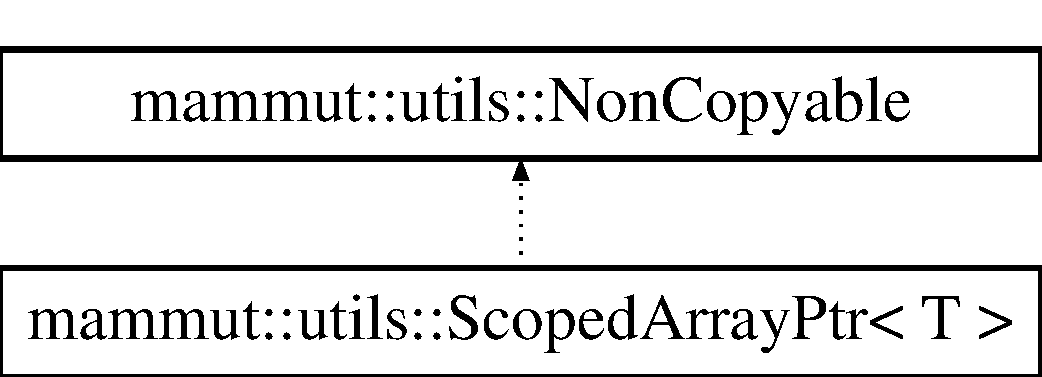
\includegraphics[height=2.000000cm]{classmammut_1_1utils_1_1ScopedArrayPtr}
\end{center}
\end{figure}
\subsection*{Public Member Functions}
\begin{DoxyCompactItemize}
\item 
\hypertarget{classmammut_1_1utils_1_1ScopedArrayPtr_ab591e38833fc647d0d5777c18ae118cf}{{\bfseries Scoped\-Array\-Ptr} (T $\ast$p=0)}\label{classmammut_1_1utils_1_1ScopedArrayPtr_ab591e38833fc647d0d5777c18ae118cf}

\end{DoxyCompactItemize}


The documentation for this class was generated from the following file\-:\begin{DoxyCompactItemize}
\item 
/home/daniele/\-Code/\-Mammut/mammut/utils.\-hpp\end{DoxyCompactItemize}

\hypertarget{classmammut_1_1utils_1_1ScopedLock}{\section{mammut\-:\-:utils\-:\-:Scoped\-Lock Class Reference}
\label{classmammut_1_1utils_1_1ScopedLock}\index{mammut\-::utils\-::\-Scoped\-Lock@{mammut\-::utils\-::\-Scoped\-Lock}}
}
Inheritance diagram for mammut\-:\-:utils\-:\-:Scoped\-Lock\-:\begin{figure}[H]
\begin{center}
\leavevmode
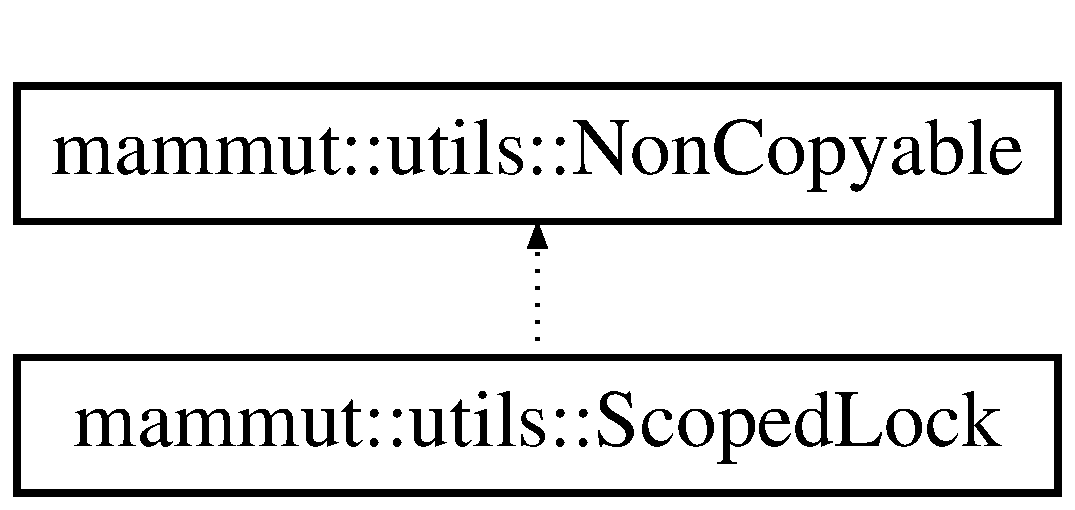
\includegraphics[height=2.000000cm]{classmammut_1_1utils_1_1ScopedLock}
\end{center}
\end{figure}
\subsection*{Public Member Functions}
\begin{DoxyCompactItemize}
\item 
\hypertarget{classmammut_1_1utils_1_1ScopedLock_a13934c56c0e4b3c54e35a01accec0ffe}{{\bfseries Scoped\-Lock} (\hyperlink{classmammut_1_1utils_1_1Lock}{Lock} \&lock)}\label{classmammut_1_1utils_1_1ScopedLock_a13934c56c0e4b3c54e35a01accec0ffe}

\end{DoxyCompactItemize}


The documentation for this class was generated from the following files\-:\begin{DoxyCompactItemize}
\item 
/home/daniele/\-Code/\-Mammut/mammut/utils.\-hpp\item 
/home/daniele/\-Code/\-Mammut/mammut/utils.\-cpp\end{DoxyCompactItemize}

\hypertarget{classmammut_1_1utils_1_1ScopedPtr}{\section{mammut\-:\-:utils\-:\-:Scoped\-Ptr$<$ T $>$ Class Template Reference}
\label{classmammut_1_1utils_1_1ScopedPtr}\index{mammut\-::utils\-::\-Scoped\-Ptr$<$ T $>$@{mammut\-::utils\-::\-Scoped\-Ptr$<$ T $>$}}
}
Inheritance diagram for mammut\-:\-:utils\-:\-:Scoped\-Ptr$<$ T $>$\-:\begin{figure}[H]
\begin{center}
\leavevmode
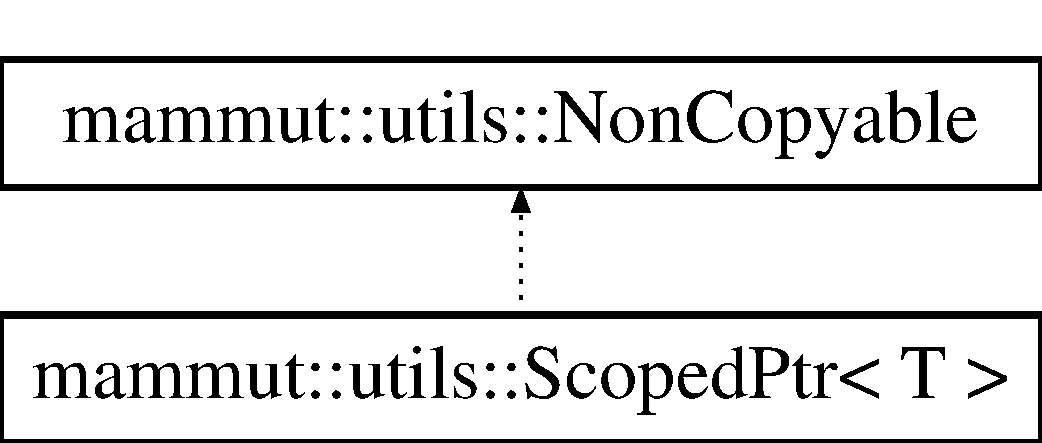
\includegraphics[height=2.000000cm]{classmammut_1_1utils_1_1ScopedPtr}
\end{center}
\end{figure}
\subsection*{Public Member Functions}
\begin{DoxyCompactItemize}
\item 
\hypertarget{classmammut_1_1utils_1_1ScopedPtr_a2cbd722886ea02740ad3b646f18df6fb}{{\bfseries Scoped\-Ptr} (T $\ast$p=0)}\label{classmammut_1_1utils_1_1ScopedPtr_a2cbd722886ea02740ad3b646f18df6fb}

\end{DoxyCompactItemize}


The documentation for this class was generated from the following file\-:\begin{DoxyCompactItemize}
\item 
/home/daniele/\-Code/\-Mammut/mammut/utils.\-hpp\end{DoxyCompactItemize}

\hypertarget{classmammut_1_1topology_1_1SpinnerThread}{\section{mammut\-:\-:topology\-:\-:Spinner\-Thread Class Reference}
\label{classmammut_1_1topology_1_1SpinnerThread}\index{mammut\-::topology\-::\-Spinner\-Thread@{mammut\-::topology\-::\-Spinner\-Thread}}
}


{\ttfamily \#include $<$topology-\/linux.\-hpp$>$}

Inheritance diagram for mammut\-:\-:topology\-:\-:Spinner\-Thread\-:\begin{figure}[H]
\begin{center}
\leavevmode
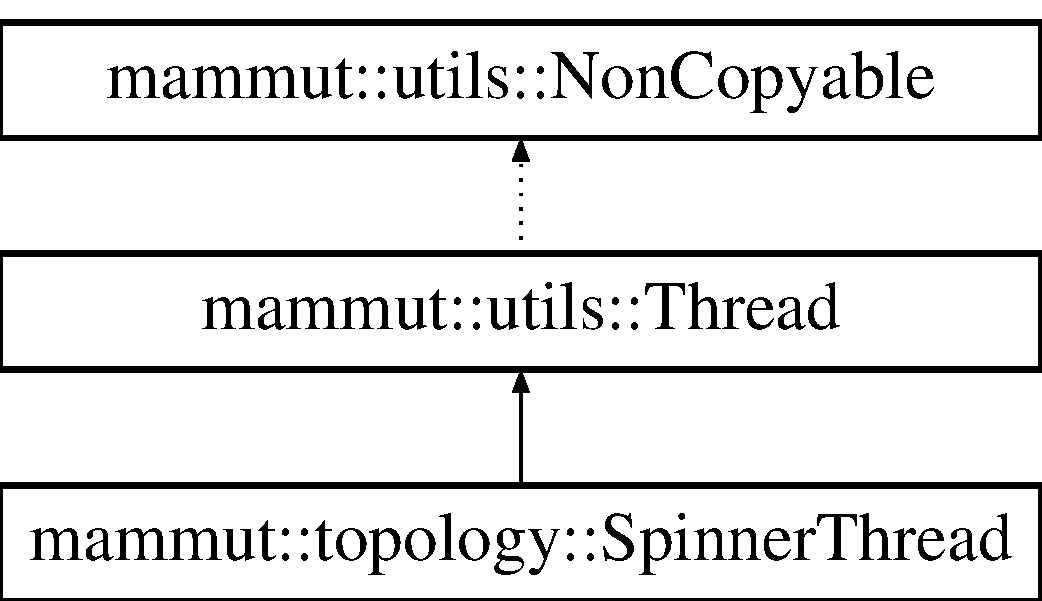
\includegraphics[height=3.000000cm]{classmammut_1_1topology_1_1SpinnerThread}
\end{center}
\end{figure}
\subsection*{Public Member Functions}
\begin{DoxyCompactItemize}
\item 
\hypertarget{classmammut_1_1topology_1_1SpinnerThread_a7a34eede0034fa73e1dc4cdb4ec6a47a}{void {\bfseries set\-Stop} (bool s)}\label{classmammut_1_1topology_1_1SpinnerThread_a7a34eede0034fa73e1dc4cdb4ec6a47a}

\item 
void \hyperlink{classmammut_1_1topology_1_1SpinnerThread_ab13fed916eab76656a92ee38b85ad6c6}{run} ()
\end{DoxyCompactItemize}


\subsection{Detailed Description}
Rise the utilization to 100\%. To start\-: set\-Stop(false); \hyperlink{classmammut_1_1utils_1_1Thread_a7c09cabe54b1626a574eca403d3f569c}{start()}; To stop\-: set\-Stop(true); \hyperlink{classmammut_1_1utils_1_1Thread_a5d5f68a806285803e815debc6dd0f278}{join()}; 

\subsection{Member Function Documentation}
\hypertarget{classmammut_1_1topology_1_1SpinnerThread_ab13fed916eab76656a92ee38b85ad6c6}{\index{mammut\-::topology\-::\-Spinner\-Thread@{mammut\-::topology\-::\-Spinner\-Thread}!run@{run}}
\index{run@{run}!mammut::topology::SpinnerThread@{mammut\-::topology\-::\-Spinner\-Thread}}
\subsubsection[{run}]{\setlength{\rightskip}{0pt plus 5cm}void mammut\-::topology\-::\-Spinner\-Thread\-::run (
\begin{DoxyParamCaption}
{}
\end{DoxyParamCaption}
)\hspace{0.3cm}{\ttfamily [virtual]}}}\label{classmammut_1_1topology_1_1SpinnerThread_ab13fed916eab76656a92ee38b85ad6c6}
This is the function that will be executed by the thread. To create a custom thread, is sufficient to extend this class and implement this pure member function. 

Implements \hyperlink{classmammut_1_1utils_1_1Thread_afc8a6df35c4f0417e6be899df973cca7}{mammut\-::utils\-::\-Thread}.



The documentation for this class was generated from the following files\-:\begin{DoxyCompactItemize}
\item 
/home/daniele/\-Code/\-Mammut/mammut/topology/topology-\/linux.\-hpp\item 
/home/daniele/\-Code/\-Mammut/mammut/topology/topology-\/linux.\-cpp\end{DoxyCompactItemize}

\hypertarget{classmammut_1_1task_1_1Task}{\section{mammut\-:\-:task\-:\-:Task Class Reference}
\label{classmammut_1_1task_1_1Task}\index{mammut\-::task\-::\-Task@{mammut\-::task\-::\-Task}}
}
Inheritance diagram for mammut\-:\-:task\-:\-:Task\-:\begin{figure}[H]
\begin{center}
\leavevmode

\includegraphics[height=2.000000cm]{classmammut_1_1task_1_1Task}
\end{center}
\end{figure}
\subsection*{Public Member Functions}
\begin{DoxyCompactItemize}
\item 
virtual bool \hyperlink{classmammut_1_1task_1_1Task_a4649012d8b17e09dc9270b61ad296d91}{get\-Core\-Usage} (double \&core\-Usage) const =0
\item 
virtual bool \hyperlink{classmammut_1_1task_1_1Task_a07b164a46a147eb76af005fa23e39826}{reset\-Core\-Usage} ()=0
\item 
virtual bool \hyperlink{classmammut_1_1task_1_1Task_a4ff24fb8519aef63e9fd0848f065733d}{get\-Priority} (uint \&priority) const =0
\item 
virtual bool \hyperlink{classmammut_1_1task_1_1Task_a6ca8b0fb237d41bdae18dd5d98ed4012}{set\-Priority} (uint priority) const =0
\item 
virtual bool \hyperlink{classmammut_1_1task_1_1Task_a8f8b0d63ca29856427735e93b039ea24}{get\-Virtual\-Core\-Id} (topology\-::\-Virtual\-Core\-Id \&virtual\-Core\-Id) const =0
\item 
virtual bool \hyperlink{classmammut_1_1task_1_1Task_a9f7366c0e1f4c0b9f02e453d18ec41a5}{move} (const \hyperlink{classmammut_1_1topology_1_1Cpu}{topology\-::\-Cpu} $\ast$cpu) const =0
\item 
virtual bool \hyperlink{classmammut_1_1task_1_1Task_ae9137276cf4b4440a66b7b310bd51466}{move} (const \hyperlink{classmammut_1_1topology_1_1PhysicalCore}{topology\-::\-Physical\-Core} $\ast$physical\-Core) const =0
\item 
virtual bool \hyperlink{classmammut_1_1task_1_1Task_a10937944c3534c4b5a21b584c9ceafb8}{move} (const \hyperlink{classmammut_1_1topology_1_1VirtualCore}{topology\-::\-Virtual\-Core} $\ast$virtual\-Core) const =0
\item 
virtual bool \hyperlink{classmammut_1_1task_1_1Task_a461a62415be252aaf4868ee781b09220}{move} (topology\-::\-Virtual\-Core\-Id virtual\-Core\-Id) const =0
\item 
virtual bool \hyperlink{classmammut_1_1task_1_1Task_afb35378fa3ebdbb92aa2875530b9cb64}{move} (const std\-::vector$<$ const \hyperlink{classmammut_1_1topology_1_1VirtualCore}{topology\-::\-Virtual\-Core} $\ast$ $>$ virtual\-Cores) const =0
\item 
virtual bool \hyperlink{classmammut_1_1task_1_1Task_af6bd70528163acb0e1c5becc7bdca326}{move} (const std\-::vector$<$ topology\-::\-Virtual\-Core\-Id $>$ virtual\-Cores\-Ids) const =0
\end{DoxyCompactItemize}


\subsection{Member Function Documentation}
\hypertarget{classmammut_1_1task_1_1Task_a4649012d8b17e09dc9270b61ad296d91}{\index{mammut\-::task\-::\-Task@{mammut\-::task\-::\-Task}!get\-Core\-Usage@{get\-Core\-Usage}}
\index{get\-Core\-Usage@{get\-Core\-Usage}!mammut::task::Task@{mammut\-::task\-::\-Task}}
\subsubsection[{get\-Core\-Usage}]{\setlength{\rightskip}{0pt plus 5cm}virtual bool mammut\-::task\-::\-Task\-::get\-Core\-Usage (
\begin{DoxyParamCaption}
\item[{double \&}]{core\-Usage}
\end{DoxyParamCaption}
) const\hspace{0.3cm}{\ttfamily [pure virtual]}}}\label{classmammut_1_1task_1_1Task_a4649012d8b17e09dc9270b61ad296d91}
Returns the percentage of time spent by this execution unit on a processing core. The percentage is computed over a period of time spanning from the last call of reset\-Core\-Usage (or from the creation of this object) to the moment of this call. 
\begin{DoxyParams}{Parameters}
{\em core\-Usage} & The percentage of time spent by this execution unit on a processing core. \\
\hline
\end{DoxyParams}
\begin{DoxyReturn}{Returns}
If false is returned, this execution unit is no more active and the call failed. Otherwise, true is returned. 
\end{DoxyReturn}
\hypertarget{classmammut_1_1task_1_1Task_a4ff24fb8519aef63e9fd0848f065733d}{\index{mammut\-::task\-::\-Task@{mammut\-::task\-::\-Task}!get\-Priority@{get\-Priority}}
\index{get\-Priority@{get\-Priority}!mammut::task::Task@{mammut\-::task\-::\-Task}}
\subsubsection[{get\-Priority}]{\setlength{\rightskip}{0pt plus 5cm}virtual bool mammut\-::task\-::\-Task\-::get\-Priority (
\begin{DoxyParamCaption}
\item[{uint \&}]{priority}
\end{DoxyParamCaption}
) const\hspace{0.3cm}{\ttfamily [pure virtual]}}}\label{classmammut_1_1task_1_1Task_a4ff24fb8519aef63e9fd0848f065733d}
Gets the current priority of this execution unit. 
\begin{DoxyParams}{Parameters}
{\em priority} & The current priority of this execution unit. The higher is the value, the higher is the priority. It will be in the range \mbox{[}M\-A\-M\-M\-U\-T\-\_\-\-P\-R\-O\-C\-E\-S\-S\-\_\-\-P\-R\-I\-O\-R\-I\-T\-Y\-\_\-\-M\-I\-N, M\-A\-M\-M\-U\-T\-\_\-\-P\-R\-O\-C\-E\-S\-S\-\_\-\-P\-R\-I\-O\-R\-I\-T\-Y\-\_\-\-M\-A\-X\mbox{]} \\
\hline
\end{DoxyParams}
\begin{DoxyReturn}{Returns}
If false is returned, this execution unit is no more active and the call failed. Otherwise, true is returned. 
\end{DoxyReturn}
\hypertarget{classmammut_1_1task_1_1Task_a8f8b0d63ca29856427735e93b039ea24}{\index{mammut\-::task\-::\-Task@{mammut\-::task\-::\-Task}!get\-Virtual\-Core\-Id@{get\-Virtual\-Core\-Id}}
\index{get\-Virtual\-Core\-Id@{get\-Virtual\-Core\-Id}!mammut::task::Task@{mammut\-::task\-::\-Task}}
\subsubsection[{get\-Virtual\-Core\-Id}]{\setlength{\rightskip}{0pt plus 5cm}virtual bool mammut\-::task\-::\-Task\-::get\-Virtual\-Core\-Id (
\begin{DoxyParamCaption}
\item[{topology\-::\-Virtual\-Core\-Id \&}]{virtual\-Core\-Id}
\end{DoxyParamCaption}
) const\hspace{0.3cm}{\ttfamily [pure virtual]}}}\label{classmammut_1_1task_1_1Task_a8f8b0d63ca29856427735e93b039ea24}
Gets the identifier of the virtual core on which this unit is currently running. 
\begin{DoxyParams}{Parameters}
{\em virtual\-Core\-Id} & The identifier of the virtual core on which this unit is currently running. \\
\hline
\end{DoxyParams}
\begin{DoxyReturn}{Returns}
If false is returned, this execution unit is no more active and the call failed. Otherwise, true is returned. 
\end{DoxyReturn}
\hypertarget{classmammut_1_1task_1_1Task_a9f7366c0e1f4c0b9f02e453d18ec41a5}{\index{mammut\-::task\-::\-Task@{mammut\-::task\-::\-Task}!move@{move}}
\index{move@{move}!mammut::task::Task@{mammut\-::task\-::\-Task}}
\subsubsection[{move}]{\setlength{\rightskip}{0pt plus 5cm}virtual bool mammut\-::task\-::\-Task\-::move (
\begin{DoxyParamCaption}
\item[{const {\bf topology\-::\-Cpu} $\ast$}]{cpu}
\end{DoxyParamCaption}
) const\hspace{0.3cm}{\ttfamily [pure virtual]}}}\label{classmammut_1_1task_1_1Task_a9f7366c0e1f4c0b9f02e453d18ec41a5}
Move this execution unit on a specified C\-P\-U. N\-O\-T\-E\-: If executed on a process, all its threads will be moved too. 
\begin{DoxyParams}{Parameters}
{\em cpu} & The C\-P\-U on which this execution unit must be moved. \\
\hline
\end{DoxyParams}
\begin{DoxyReturn}{Returns}
If false is returned, this execution unit is no more active and the call failed. Otherwise, true is returned. 
\end{DoxyReturn}
\hypertarget{classmammut_1_1task_1_1Task_ae9137276cf4b4440a66b7b310bd51466}{\index{mammut\-::task\-::\-Task@{mammut\-::task\-::\-Task}!move@{move}}
\index{move@{move}!mammut::task::Task@{mammut\-::task\-::\-Task}}
\subsubsection[{move}]{\setlength{\rightskip}{0pt plus 5cm}virtual bool mammut\-::task\-::\-Task\-::move (
\begin{DoxyParamCaption}
\item[{const {\bf topology\-::\-Physical\-Core} $\ast$}]{physical\-Core}
\end{DoxyParamCaption}
) const\hspace{0.3cm}{\ttfamily [pure virtual]}}}\label{classmammut_1_1task_1_1Task_ae9137276cf4b4440a66b7b310bd51466}
Move this execution unit on a specified physical core. N\-O\-T\-E\-: If executed on a process, all its threads will be moved too. 
\begin{DoxyParams}{Parameters}
{\em physical\-Core} & The physical core on which this execution unit must be moved. \\
\hline
\end{DoxyParams}
\begin{DoxyReturn}{Returns}
If false is returned, this execution unit is no more active and the call failed. Otherwise, true is returned. 
\end{DoxyReturn}
\hypertarget{classmammut_1_1task_1_1Task_a10937944c3534c4b5a21b584c9ceafb8}{\index{mammut\-::task\-::\-Task@{mammut\-::task\-::\-Task}!move@{move}}
\index{move@{move}!mammut::task::Task@{mammut\-::task\-::\-Task}}
\subsubsection[{move}]{\setlength{\rightskip}{0pt plus 5cm}virtual bool mammut\-::task\-::\-Task\-::move (
\begin{DoxyParamCaption}
\item[{const {\bf topology\-::\-Virtual\-Core} $\ast$}]{virtual\-Core}
\end{DoxyParamCaption}
) const\hspace{0.3cm}{\ttfamily [pure virtual]}}}\label{classmammut_1_1task_1_1Task_a10937944c3534c4b5a21b584c9ceafb8}
Move this execution unit on a specified virtual core. N\-O\-T\-E\-: If executed on a process, all its threads will be moved too. 
\begin{DoxyParams}{Parameters}
{\em virtual\-Core} & The virtual core on which this execution unit must be moved. \\
\hline
\end{DoxyParams}
\begin{DoxyReturn}{Returns}
If false is returned, this execution unit is no more active and the call failed. Otherwise, true is returned. 
\end{DoxyReturn}
\hypertarget{classmammut_1_1task_1_1Task_a461a62415be252aaf4868ee781b09220}{\index{mammut\-::task\-::\-Task@{mammut\-::task\-::\-Task}!move@{move}}
\index{move@{move}!mammut::task::Task@{mammut\-::task\-::\-Task}}
\subsubsection[{move}]{\setlength{\rightskip}{0pt plus 5cm}virtual bool mammut\-::task\-::\-Task\-::move (
\begin{DoxyParamCaption}
\item[{topology\-::\-Virtual\-Core\-Id}]{virtual\-Core\-Id}
\end{DoxyParamCaption}
) const\hspace{0.3cm}{\ttfamily [pure virtual]}}}\label{classmammut_1_1task_1_1Task_a461a62415be252aaf4868ee781b09220}
Move this execution unit on a specified virtual core. N\-O\-T\-E\-: If executed on a process, all its threads will be moved too. 
\begin{DoxyParams}{Parameters}
{\em virtual\-Core\-Id} & The identifier of the virtual core on which this execution unit must be moved. \\
\hline
\end{DoxyParams}
\begin{DoxyReturn}{Returns}
If false is returned, this execution unit is no more active and the call failed. Otherwise, true is returned. 
\end{DoxyReturn}
\hypertarget{classmammut_1_1task_1_1Task_afb35378fa3ebdbb92aa2875530b9cb64}{\index{mammut\-::task\-::\-Task@{mammut\-::task\-::\-Task}!move@{move}}
\index{move@{move}!mammut::task::Task@{mammut\-::task\-::\-Task}}
\subsubsection[{move}]{\setlength{\rightskip}{0pt plus 5cm}virtual bool mammut\-::task\-::\-Task\-::move (
\begin{DoxyParamCaption}
\item[{const std\-::vector$<$ const {\bf topology\-::\-Virtual\-Core} $\ast$ $>$}]{virtual\-Cores}
\end{DoxyParamCaption}
) const\hspace{0.3cm}{\ttfamily [pure virtual]}}}\label{classmammut_1_1task_1_1Task_afb35378fa3ebdbb92aa2875530b9cb64}
Move this execution unit on a set of specified virtual cores. 
\begin{DoxyParams}{Parameters}
{\em virtual\-Cores} & The virtual cores on which this execution unit must be moved. \\
\hline
\end{DoxyParams}
\begin{DoxyReturn}{Returns}
If false is returned, this execution unit is no more active and the call failed. Otherwise, true is returned. 
\end{DoxyReturn}
\hypertarget{classmammut_1_1task_1_1Task_af6bd70528163acb0e1c5becc7bdca326}{\index{mammut\-::task\-::\-Task@{mammut\-::task\-::\-Task}!move@{move}}
\index{move@{move}!mammut::task::Task@{mammut\-::task\-::\-Task}}
\subsubsection[{move}]{\setlength{\rightskip}{0pt plus 5cm}virtual bool mammut\-::task\-::\-Task\-::move (
\begin{DoxyParamCaption}
\item[{const std\-::vector$<$ topology\-::\-Virtual\-Core\-Id $>$}]{virtual\-Cores\-Ids}
\end{DoxyParamCaption}
) const\hspace{0.3cm}{\ttfamily [pure virtual]}}}\label{classmammut_1_1task_1_1Task_af6bd70528163acb0e1c5becc7bdca326}
Move this execution unit on a set of specified virtual cores. 
\begin{DoxyParams}{Parameters}
{\em virtual\-Cores\-Ids} & The identifiers of the virtual cores on which this execution unit must be moved. \\
\hline
\end{DoxyParams}
\begin{DoxyReturn}{Returns}
If false is returned, this execution unit is no more active and the call failed. Otherwise, true is returned. 
\end{DoxyReturn}
\hypertarget{classmammut_1_1task_1_1Task_a07b164a46a147eb76af005fa23e39826}{\index{mammut\-::task\-::\-Task@{mammut\-::task\-::\-Task}!reset\-Core\-Usage@{reset\-Core\-Usage}}
\index{reset\-Core\-Usage@{reset\-Core\-Usage}!mammut::task::Task@{mammut\-::task\-::\-Task}}
\subsubsection[{reset\-Core\-Usage}]{\setlength{\rightskip}{0pt plus 5cm}virtual bool mammut\-::task\-::\-Task\-::reset\-Core\-Usage (
\begin{DoxyParamCaption}
{}
\end{DoxyParamCaption}
)\hspace{0.3cm}{\ttfamily [pure virtual]}}}\label{classmammut_1_1task_1_1Task_a07b164a46a147eb76af005fa23e39826}
Resets the counter for core usage percentage computation. \begin{DoxyReturn}{Returns}
If false is returned, this execution unit is no more active and the call failed. Otherwise, true is returned. 
\end{DoxyReturn}
\hypertarget{classmammut_1_1task_1_1Task_a6ca8b0fb237d41bdae18dd5d98ed4012}{\index{mammut\-::task\-::\-Task@{mammut\-::task\-::\-Task}!set\-Priority@{set\-Priority}}
\index{set\-Priority@{set\-Priority}!mammut::task::Task@{mammut\-::task\-::\-Task}}
\subsubsection[{set\-Priority}]{\setlength{\rightskip}{0pt plus 5cm}virtual bool mammut\-::task\-::\-Task\-::set\-Priority (
\begin{DoxyParamCaption}
\item[{uint}]{priority}
\end{DoxyParamCaption}
) const\hspace{0.3cm}{\ttfamily [pure virtual]}}}\label{classmammut_1_1task_1_1Task_a6ca8b0fb237d41bdae18dd5d98ed4012}
Sets the priority of this execution unit. N\-O\-T\-E\-: If executed on a process, the priority of all its thread will be changed too. N\-O\-T\-E\-: It may require privileged rights. 
\begin{DoxyParams}{Parameters}
{\em priority} & The priority of this execution unit. The higher is the value, the higher is the priority. It must be in the range \mbox{[}M\-A\-M\-M\-U\-T\-\_\-\-P\-R\-O\-C\-E\-S\-S\-\_\-\-P\-R\-I\-O\-R\-I\-T\-Y\-\_\-\-M\-I\-N, M\-A\-M\-M\-U\-T\-\_\-\-P\-R\-O\-C\-E\-S\-S\-\_\-\-P\-R\-I\-O\-R\-I\-T\-Y\-\_\-\-M\-A\-X\mbox{]} \\
\hline
\end{DoxyParams}
\begin{DoxyReturn}{Returns}
If false is returned, the priority value is outside the allowed range or this execution unit is no more active and the call failed. Otherwise, true is returned. 
\end{DoxyReturn}


The documentation for this class was generated from the following file\-:\begin{DoxyCompactItemize}
\item 
/home/daniele/\-Code/\-Mammut/mammut/task/task.\-hpp\end{DoxyCompactItemize}

\hypertarget{classmammut_1_1task_1_1TasksManager}{\section{mammut\-:\-:task\-:\-:Tasks\-Manager Class Reference}
\label{classmammut_1_1task_1_1TasksManager}\index{mammut\-::task\-::\-Tasks\-Manager@{mammut\-::task\-::\-Tasks\-Manager}}
}
Inheritance diagram for mammut\-:\-:task\-:\-:Tasks\-Manager\-:\begin{figure}[H]
\begin{center}
\leavevmode
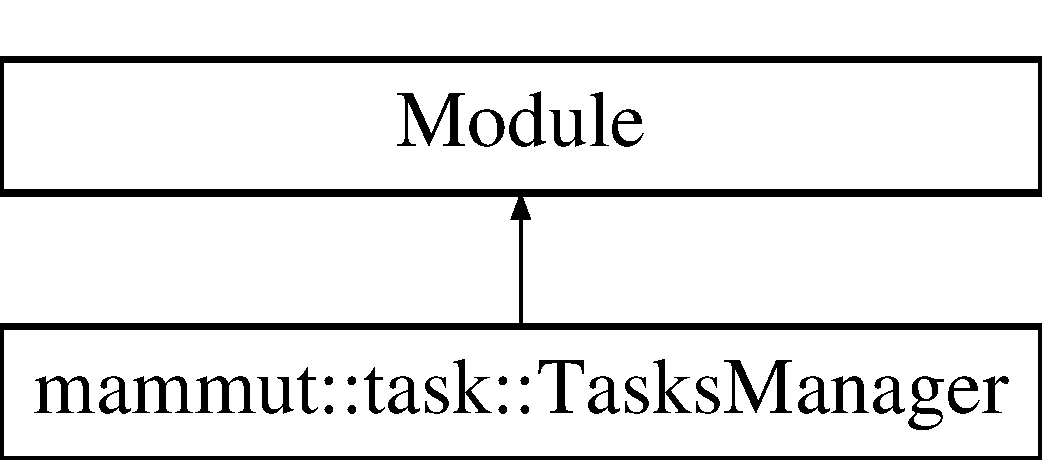
\includegraphics[height=2.000000cm]{classmammut_1_1task_1_1TasksManager}
\end{center}
\end{figure}
\subsection*{Public Member Functions}
\begin{DoxyCompactItemize}
\item 
virtual std\-::vector$<$ Task\-Id $>$ \hyperlink{classmammut_1_1task_1_1TasksManager_a301de447218cce0ae1f81af943ea6fe5}{get\-Active\-Processes\-Identifiers} () const =0
\item 
virtual \hyperlink{classmammut_1_1task_1_1ProcessHandler}{Process\-Handler} $\ast$ \hyperlink{classmammut_1_1task_1_1TasksManager_a529f75258ad54951209786ebfec1d658}{get\-Process\-Handler} (Task\-Id pid) const =0
\item 
virtual void \hyperlink{classmammut_1_1task_1_1TasksManager_ad97b2200f285f63f6e8858cce31422d3}{release\-Process\-Handler} (\hyperlink{classmammut_1_1task_1_1ProcessHandler}{Process\-Handler} $\ast$process) const =0
\item 
virtual \hyperlink{classmammut_1_1task_1_1ThreadHandler}{Thread\-Handler} $\ast$ \hyperlink{classmammut_1_1task_1_1TasksManager_a3c4a48df7d66c4fcf56c055d951d6bbe}{get\-Thread\-Handler} (Task\-Id pid, Task\-Id tid) const =0
\item 
virtual \hyperlink{classmammut_1_1task_1_1ThreadHandler}{Thread\-Handler} $\ast$ \hyperlink{classmammut_1_1task_1_1TasksManager_abf218ec9437ec3b6e2257715063b7262}{get\-Thread\-Handler} () const =0
\item 
virtual void \hyperlink{classmammut_1_1task_1_1TasksManager_af5ad5db5b43441a49e0a5633dd1ff667}{release\-Thread\-Handler} (\hyperlink{classmammut_1_1task_1_1ThreadHandler}{Thread\-Handler} $\ast$thread) const =0
\end{DoxyCompactItemize}


\subsection{Member Function Documentation}
\hypertarget{classmammut_1_1task_1_1TasksManager_a301de447218cce0ae1f81af943ea6fe5}{\index{mammut\-::task\-::\-Tasks\-Manager@{mammut\-::task\-::\-Tasks\-Manager}!get\-Active\-Processes\-Identifiers@{get\-Active\-Processes\-Identifiers}}
\index{get\-Active\-Processes\-Identifiers@{get\-Active\-Processes\-Identifiers}!mammut::task::TasksManager@{mammut\-::task\-::\-Tasks\-Manager}}
\subsubsection[{get\-Active\-Processes\-Identifiers}]{\setlength{\rightskip}{0pt plus 5cm}virtual std\-::vector$<$Task\-Id$>$ mammut\-::task\-::\-Tasks\-Manager\-::get\-Active\-Processes\-Identifiers (
\begin{DoxyParamCaption}
{}
\end{DoxyParamCaption}
) const\hspace{0.3cm}{\ttfamily [pure virtual]}}}\label{classmammut_1_1task_1_1TasksManager_a301de447218cce0ae1f81af943ea6fe5}
Returns a list of active processes identifiers. \begin{DoxyReturn}{Returns}
A vector of active processes identifiers. 
\end{DoxyReturn}
\hypertarget{classmammut_1_1task_1_1TasksManager_a529f75258ad54951209786ebfec1d658}{\index{mammut\-::task\-::\-Tasks\-Manager@{mammut\-::task\-::\-Tasks\-Manager}!get\-Process\-Handler@{get\-Process\-Handler}}
\index{get\-Process\-Handler@{get\-Process\-Handler}!mammut::task::TasksManager@{mammut\-::task\-::\-Tasks\-Manager}}
\subsubsection[{get\-Process\-Handler}]{\setlength{\rightskip}{0pt plus 5cm}virtual {\bf Process\-Handler}$\ast$ mammut\-::task\-::\-Tasks\-Manager\-::get\-Process\-Handler (
\begin{DoxyParamCaption}
\item[{Task\-Id}]{pid}
\end{DoxyParamCaption}
) const\hspace{0.3cm}{\ttfamily [pure virtual]}}}\label{classmammut_1_1task_1_1TasksManager_a529f75258ad54951209786ebfec1d658}
Returns the handler associated to a specific process. 
\begin{DoxyParams}{Parameters}
{\em pid} & The process identifier. \\
\hline
\end{DoxyParams}
\begin{DoxyReturn}{Returns}
The handler associated to a specific process or N\-U\-L\-L if the process doesn't exists. The obtained handler must be released with release\-Process\-Handler call. 
\end{DoxyReturn}
\hypertarget{classmammut_1_1task_1_1TasksManager_a3c4a48df7d66c4fcf56c055d951d6bbe}{\index{mammut\-::task\-::\-Tasks\-Manager@{mammut\-::task\-::\-Tasks\-Manager}!get\-Thread\-Handler@{get\-Thread\-Handler}}
\index{get\-Thread\-Handler@{get\-Thread\-Handler}!mammut::task::TasksManager@{mammut\-::task\-::\-Tasks\-Manager}}
\subsubsection[{get\-Thread\-Handler}]{\setlength{\rightskip}{0pt plus 5cm}virtual {\bf Thread\-Handler}$\ast$ mammut\-::task\-::\-Tasks\-Manager\-::get\-Thread\-Handler (
\begin{DoxyParamCaption}
\item[{Task\-Id}]{pid, }
\item[{Task\-Id}]{tid}
\end{DoxyParamCaption}
) const\hspace{0.3cm}{\ttfamily [pure virtual]}}}\label{classmammut_1_1task_1_1TasksManager_a3c4a48df7d66c4fcf56c055d951d6bbe}
Returns the handler associated to a specific thread. 
\begin{DoxyParams}{Parameters}
{\em pid} & The process identifier. \\
\hline
{\em tid} & The thread identifier. \\
\hline
\end{DoxyParams}
\begin{DoxyReturn}{Returns}
The handler associated to a specific thread or N\-U\-L\-L if the thread doesn't exists. The obtained handler must be released with release\-Thread\-Handler call. 
\end{DoxyReturn}
\hypertarget{classmammut_1_1task_1_1TasksManager_abf218ec9437ec3b6e2257715063b7262}{\index{mammut\-::task\-::\-Tasks\-Manager@{mammut\-::task\-::\-Tasks\-Manager}!get\-Thread\-Handler@{get\-Thread\-Handler}}
\index{get\-Thread\-Handler@{get\-Thread\-Handler}!mammut::task::TasksManager@{mammut\-::task\-::\-Tasks\-Manager}}
\subsubsection[{get\-Thread\-Handler}]{\setlength{\rightskip}{0pt plus 5cm}virtual {\bf Thread\-Handler}$\ast$ mammut\-::task\-::\-Tasks\-Manager\-::get\-Thread\-Handler (
\begin{DoxyParamCaption}
{}
\end{DoxyParamCaption}
) const\hspace{0.3cm}{\ttfamily [pure virtual]}}}\label{classmammut_1_1task_1_1TasksManager_abf218ec9437ec3b6e2257715063b7262}
Returns the handler associated to the calling thread. \begin{DoxyReturn}{Returns}
The handler associated to the calling thread. The obtained handler must be released with release\-Thread\-Handler call. 
\end{DoxyReturn}
\hypertarget{classmammut_1_1task_1_1TasksManager_ad97b2200f285f63f6e8858cce31422d3}{\index{mammut\-::task\-::\-Tasks\-Manager@{mammut\-::task\-::\-Tasks\-Manager}!release\-Process\-Handler@{release\-Process\-Handler}}
\index{release\-Process\-Handler@{release\-Process\-Handler}!mammut::task::TasksManager@{mammut\-::task\-::\-Tasks\-Manager}}
\subsubsection[{release\-Process\-Handler}]{\setlength{\rightskip}{0pt plus 5cm}virtual void mammut\-::task\-::\-Tasks\-Manager\-::release\-Process\-Handler (
\begin{DoxyParamCaption}
\item[{{\bf Process\-Handler} $\ast$}]{process}
\end{DoxyParamCaption}
) const\hspace{0.3cm}{\ttfamily [pure virtual]}}}\label{classmammut_1_1task_1_1TasksManager_ad97b2200f285f63f6e8858cce31422d3}
Releases the handler obtained through get\-Process\-Handler call. 
\begin{DoxyParams}{Parameters}
{\em process} & The process handler. \\
\hline
\end{DoxyParams}
\hypertarget{classmammut_1_1task_1_1TasksManager_af5ad5db5b43441a49e0a5633dd1ff667}{\index{mammut\-::task\-::\-Tasks\-Manager@{mammut\-::task\-::\-Tasks\-Manager}!release\-Thread\-Handler@{release\-Thread\-Handler}}
\index{release\-Thread\-Handler@{release\-Thread\-Handler}!mammut::task::TasksManager@{mammut\-::task\-::\-Tasks\-Manager}}
\subsubsection[{release\-Thread\-Handler}]{\setlength{\rightskip}{0pt plus 5cm}virtual void mammut\-::task\-::\-Tasks\-Manager\-::release\-Thread\-Handler (
\begin{DoxyParamCaption}
\item[{{\bf Thread\-Handler} $\ast$}]{thread}
\end{DoxyParamCaption}
) const\hspace{0.3cm}{\ttfamily [pure virtual]}}}\label{classmammut_1_1task_1_1TasksManager_af5ad5db5b43441a49e0a5633dd1ff667}
Releases the handler obtained through get\-Thread\-Handler call. 
\begin{DoxyParams}{Parameters}
{\em thread} & The thread handler. \\
\hline
\end{DoxyParams}


The documentation for this class was generated from the following file\-:\begin{DoxyCompactItemize}
\item 
/home/daniele/\-Code/\-Mammut/mammut/task/task.\-hpp\end{DoxyCompactItemize}

\hypertarget{classmammut_1_1utils_1_1Thread}{\section{mammut\-:\-:utils\-:\-:Thread Class Reference}
\label{classmammut_1_1utils_1_1Thread}\index{mammut\-::utils\-::\-Thread@{mammut\-::utils\-::\-Thread}}
}
Inheritance diagram for mammut\-:\-:utils\-:\-:Thread\-:\begin{figure}[H]
\begin{center}
\leavevmode
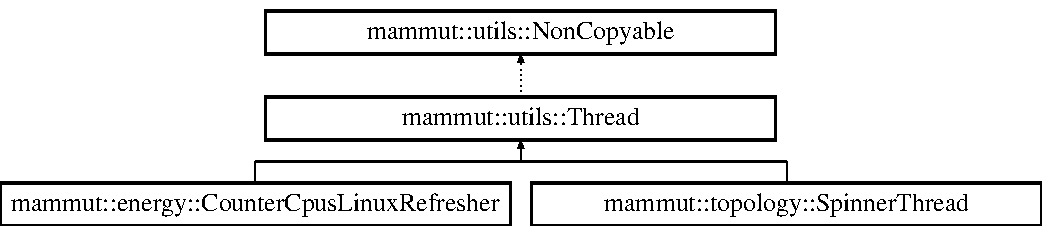
\includegraphics[height=3.000000cm]{classmammut_1_1utils_1_1Thread}
\end{center}
\end{figure}
\subsection*{Public Member Functions}
\begin{DoxyCompactItemize}
\item 
void \hyperlink{classmammut_1_1utils_1_1Thread_a7c09cabe54b1626a574eca403d3f569c}{start} ()
\item 
\hyperlink{classmammut_1_1task_1_1ThreadHandler}{mammut\-::task\-::\-Thread\-Handler} $\ast$ \hyperlink{classmammut_1_1utils_1_1Thread_aace614531a18e9d456abcd5ca4d460db}{get\-Thread\-Handler} () const 
\item 
bool \hyperlink{classmammut_1_1utils_1_1Thread_ab24ad2bd0b96b4a27420471d9e863e04}{running} ()
\item 
void \hyperlink{classmammut_1_1utils_1_1Thread_a5d5f68a806285803e815debc6dd0f278}{join} ()
\item 
virtual void \hyperlink{classmammut_1_1utils_1_1Thread_afc8a6df35c4f0417e6be899df973cca7}{run} ()=0
\end{DoxyCompactItemize}


\subsection{Member Function Documentation}
\hypertarget{classmammut_1_1utils_1_1Thread_aace614531a18e9d456abcd5ca4d460db}{\index{mammut\-::utils\-::\-Thread@{mammut\-::utils\-::\-Thread}!get\-Thread\-Handler@{get\-Thread\-Handler}}
\index{get\-Thread\-Handler@{get\-Thread\-Handler}!mammut::utils::Thread@{mammut\-::utils\-::\-Thread}}
\subsubsection[{get\-Thread\-Handler}]{\setlength{\rightskip}{0pt plus 5cm}{\bf mammut\-::task\-::\-Thread\-Handler} $\ast$ mammut\-::utils\-::\-Thread\-::get\-Thread\-Handler (
\begin{DoxyParamCaption}
{}
\end{DoxyParamCaption}
) const}}\label{classmammut_1_1utils_1_1Thread_aace614531a18e9d456abcd5ca4d460db}
Returns the thread handler associated to this thread. It is automatically released when this thread is joined. \begin{DoxyReturn}{Returns}
The thread handler associated to this thread. If this thread is not yet started (or if it finished its execution) N\-U\-L\-L is returned. 
\end{DoxyReturn}
\hypertarget{classmammut_1_1utils_1_1Thread_a5d5f68a806285803e815debc6dd0f278}{\index{mammut\-::utils\-::\-Thread@{mammut\-::utils\-::\-Thread}!join@{join}}
\index{join@{join}!mammut::utils::Thread@{mammut\-::utils\-::\-Thread}}
\subsubsection[{join}]{\setlength{\rightskip}{0pt plus 5cm}void mammut\-::utils\-::\-Thread\-::join (
\begin{DoxyParamCaption}
{}
\end{DoxyParamCaption}
)}}\label{classmammut_1_1utils_1_1Thread_a5d5f68a806285803e815debc6dd0f278}
Joins this thread. After this operation, the handler obtained with \hyperlink{classmammut_1_1utils_1_1Thread_aace614531a18e9d456abcd5ca4d460db}{get\-Thread\-Handler()} call is no more valid. \hypertarget{classmammut_1_1utils_1_1Thread_afc8a6df35c4f0417e6be899df973cca7}{\index{mammut\-::utils\-::\-Thread@{mammut\-::utils\-::\-Thread}!run@{run}}
\index{run@{run}!mammut::utils::Thread@{mammut\-::utils\-::\-Thread}}
\subsubsection[{run}]{\setlength{\rightskip}{0pt plus 5cm}virtual void mammut\-::utils\-::\-Thread\-::run (
\begin{DoxyParamCaption}
{}
\end{DoxyParamCaption}
)\hspace{0.3cm}{\ttfamily [pure virtual]}}}\label{classmammut_1_1utils_1_1Thread_afc8a6df35c4f0417e6be899df973cca7}
This is the function that will be executed by the thread. To create a custom thread, is sufficient to extend this class and implement this pure member function. 

Implemented in \hyperlink{classmammut_1_1topology_1_1SpinnerThread_ab13fed916eab76656a92ee38b85ad6c6}{mammut\-::topology\-::\-Spinner\-Thread}, and \hyperlink{classmammut_1_1energy_1_1CounterCpusLinuxRefresher_a9037ed7260ba2eea4995ac35dc079eeb}{mammut\-::energy\-::\-Counter\-Cpus\-Linux\-Refresher}.

\hypertarget{classmammut_1_1utils_1_1Thread_ab24ad2bd0b96b4a27420471d9e863e04}{\index{mammut\-::utils\-::\-Thread@{mammut\-::utils\-::\-Thread}!running@{running}}
\index{running@{running}!mammut::utils::Thread@{mammut\-::utils\-::\-Thread}}
\subsubsection[{running}]{\setlength{\rightskip}{0pt plus 5cm}bool mammut\-::utils\-::\-Thread\-::running (
\begin{DoxyParamCaption}
{}
\end{DoxyParamCaption}
)}}\label{classmammut_1_1utils_1_1Thread_ab24ad2bd0b96b4a27420471d9e863e04}
Checks if the thread is still running. \begin{DoxyReturn}{Returns}
True if the thread is still running, false otherwise. 
\end{DoxyReturn}
\hypertarget{classmammut_1_1utils_1_1Thread_a7c09cabe54b1626a574eca403d3f569c}{\index{mammut\-::utils\-::\-Thread@{mammut\-::utils\-::\-Thread}!start@{start}}
\index{start@{start}!mammut::utils::Thread@{mammut\-::utils\-::\-Thread}}
\subsubsection[{start}]{\setlength{\rightskip}{0pt plus 5cm}void mammut\-::utils\-::\-Thread\-::start (
\begin{DoxyParamCaption}
{}
\end{DoxyParamCaption}
)}}\label{classmammut_1_1utils_1_1Thread_a7c09cabe54b1626a574eca403d3f569c}
Starts this thread. A\-T\-T\-E\-N\-T\-I\-O\-N\-: When the object is deallocated the thread will keep running. It must E\-X\-P\-L\-I\-C\-I\-T\-L\-Y be joined before the object goes out of scope. 
\begin{DoxyParams}{Parameters}
{\em virtual\-Core\-Id} & The virtual core on which this thread must be mapped. \\
\hline
{\em priority} & The priority of this thread. \\
\hline
\end{DoxyParams}


The documentation for this class was generated from the following files\-:\begin{DoxyCompactItemize}
\item 
/home/daniele/\-Code/\-Mammut/mammut/utils.\-hpp\item 
/home/daniele/\-Code/\-Mammut/mammut/utils.\-cpp\end{DoxyCompactItemize}

\hypertarget{classmammut_1_1task_1_1ThreadHandler}{\section{mammut\-:\-:task\-:\-:Thread\-Handler Class Reference}
\label{classmammut_1_1task_1_1ThreadHandler}\index{mammut\-::task\-::\-Thread\-Handler@{mammut\-::task\-::\-Thread\-Handler}}
}
Inheritance diagram for mammut\-:\-:task\-:\-:Thread\-Handler\-:\begin{figure}[H]
\begin{center}
\leavevmode
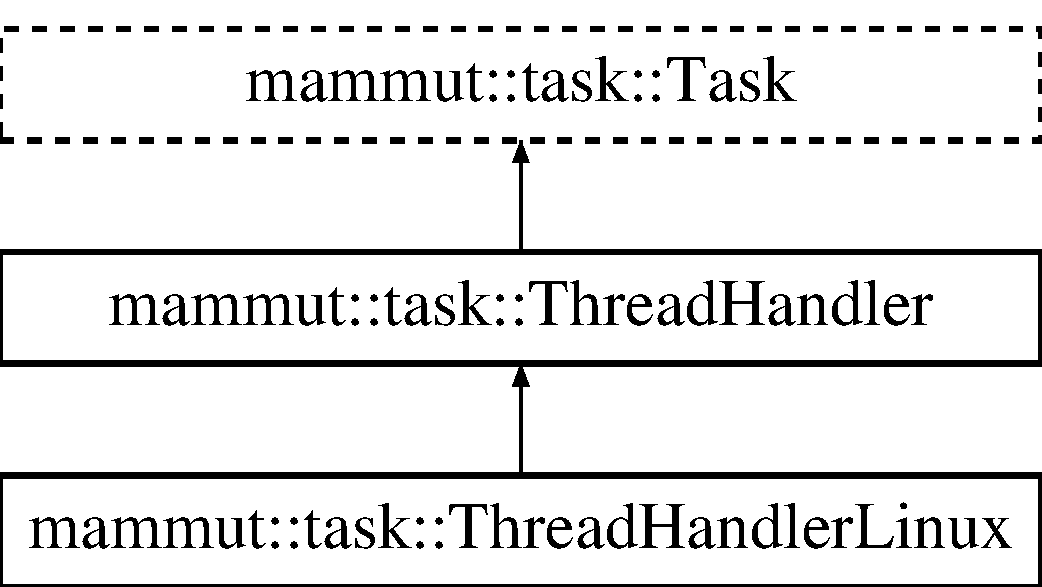
\includegraphics[height=3.000000cm]{classmammut_1_1task_1_1ThreadHandler}
\end{center}
\end{figure}
\subsection*{Additional Inherited Members}


The documentation for this class was generated from the following file\-:\begin{DoxyCompactItemize}
\item 
/home/daniele/\-Code/\-Mammut/mammut/task/task.\-hpp\end{DoxyCompactItemize}

\hypertarget{classmammut_1_1task_1_1ThreadHandlerLinux}{\section{mammut\-:\-:task\-:\-:Thread\-Handler\-Linux Class Reference}
\label{classmammut_1_1task_1_1ThreadHandlerLinux}\index{mammut\-::task\-::\-Thread\-Handler\-Linux@{mammut\-::task\-::\-Thread\-Handler\-Linux}}
}
Inheritance diagram for mammut\-:\-:task\-:\-:Thread\-Handler\-Linux\-:\begin{figure}[H]
\begin{center}
\leavevmode
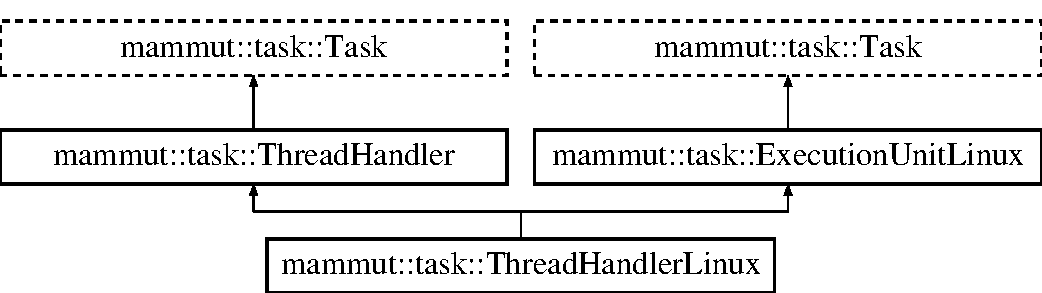
\includegraphics[height=3.000000cm]{classmammut_1_1task_1_1ThreadHandlerLinux}
\end{center}
\end{figure}
\subsection*{Public Member Functions}
\begin{DoxyCompactItemize}
\item 
\hypertarget{classmammut_1_1task_1_1ThreadHandlerLinux_a68abb28c8b0ee658cc07037548c26be0}{{\bfseries Thread\-Handler\-Linux} (Task\-Id pid, Task\-Id tid)}\label{classmammut_1_1task_1_1ThreadHandlerLinux_a68abb28c8b0ee658cc07037548c26be0}

\item 
bool \hyperlink{classmammut_1_1task_1_1ThreadHandlerLinux_a7ecc4783d78c0fdfc337800598b0165c}{move} (const std\-::vector$<$ topology\-::\-Virtual\-Core\-Id $>$ virtual\-Cores\-Ids) const 
\end{DoxyCompactItemize}


\subsection{Member Function Documentation}
\hypertarget{classmammut_1_1task_1_1ThreadHandlerLinux_a7ecc4783d78c0fdfc337800598b0165c}{\index{mammut\-::task\-::\-Thread\-Handler\-Linux@{mammut\-::task\-::\-Thread\-Handler\-Linux}!move@{move}}
\index{move@{move}!mammut::task::ThreadHandlerLinux@{mammut\-::task\-::\-Thread\-Handler\-Linux}}
\subsubsection[{move}]{\setlength{\rightskip}{0pt plus 5cm}bool mammut\-::task\-::\-Thread\-Handler\-Linux\-::move (
\begin{DoxyParamCaption}
\item[{const std\-::vector$<$ topology\-::\-Virtual\-Core\-Id $>$}]{virtual\-Cores\-Ids}
\end{DoxyParamCaption}
) const\hspace{0.3cm}{\ttfamily [virtual]}}}\label{classmammut_1_1task_1_1ThreadHandlerLinux_a7ecc4783d78c0fdfc337800598b0165c}
Move this execution unit on a set of specified virtual cores. 
\begin{DoxyParams}{Parameters}
{\em virtual\-Cores\-Ids} & The identifiers of the virtual cores on which this execution unit must be moved. \\
\hline
\end{DoxyParams}
\begin{DoxyReturn}{Returns}
If false is returned, this execution unit is no more active and the call failed. Otherwise, true is returned. 
\end{DoxyReturn}


Implements \hyperlink{classmammut_1_1task_1_1ExecutionUnitLinux_aedac673e0c581fcbfc6b3fb5a38cd81b}{mammut\-::task\-::\-Execution\-Unit\-Linux}.



The documentation for this class was generated from the following files\-:\begin{DoxyCompactItemize}
\item 
/home/daniele/\-Code/\-Mammut/mammut/task/task-\/linux.\-hpp\item 
/home/daniele/\-Code/\-Mammut/mammut/task/task-\/linux.\-cpp\end{DoxyCompactItemize}

\hypertarget{classmammut_1_1topology_1_1Topology}{\section{mammut\-:\-:topology\-:\-:Topology Class Reference}
\label{classmammut_1_1topology_1_1Topology}\index{mammut\-::topology\-::\-Topology@{mammut\-::topology\-::\-Topology}}
}
Inheritance diagram for mammut\-:\-:topology\-:\-:Topology\-:\begin{figure}[H]
\begin{center}
\leavevmode
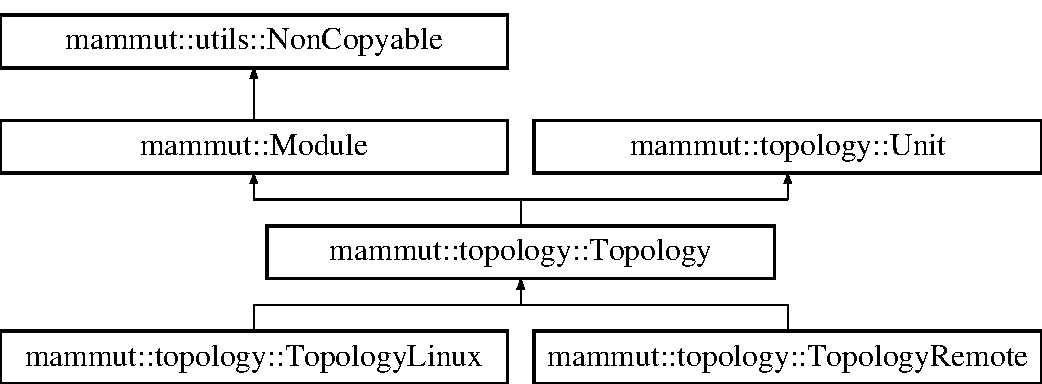
\includegraphics[height=2.000000cm]{classmammut_1_1topology_1_1Topology}
\end{center}
\end{figure}
\subsection*{Public Member Functions}
\begin{DoxyCompactItemize}
\item 
std\-::vector$<$ \hyperlink{classmammut_1_1topology_1_1Cpu}{Cpu} $\ast$ $>$ \hyperlink{classmammut_1_1topology_1_1Topology_aeb4616d9aa50bfd992f5a335688552c9}{get\-Cpus} () const 
\item 
std\-::vector$<$ \hyperlink{classmammut_1_1topology_1_1PhysicalCore}{Physical\-Core} $\ast$ $>$ \hyperlink{classmammut_1_1topology_1_1Topology_a6644abd6f67a074997336af59cf42df4}{get\-Physical\-Cores} () const 
\item 
std\-::vector$<$ \hyperlink{classmammut_1_1topology_1_1VirtualCore}{Virtual\-Core} $\ast$ $>$ \hyperlink{classmammut_1_1topology_1_1Topology_afb23140b03b50b99cd08dc7a711a0c9e}{get\-Virtual\-Cores} () const 
\item 
std\-::vector$<$ \hyperlink{classmammut_1_1topology_1_1PhysicalCore}{Physical\-Core} $\ast$ $>$ \hyperlink{classmammut_1_1topology_1_1Topology_a65ec01bacc68046bf4b4f8e5077a8664}{virtual\-To\-Physical} (const std\-::vector$<$ \hyperlink{classmammut_1_1topology_1_1VirtualCore}{Virtual\-Core} $\ast$ $>$ \&virtual\-Cores) const 
\item 
\hyperlink{classmammut_1_1topology_1_1Cpu}{Cpu} $\ast$ \hyperlink{classmammut_1_1topology_1_1Topology_a1966810401123e9102866618b2f21339}{get\-Cpu} (Cpu\-Id cpu\-Id) const 
\item 
\hyperlink{classmammut_1_1topology_1_1PhysicalCore}{Physical\-Core} $\ast$ \hyperlink{classmammut_1_1topology_1_1Topology_a36b26297620a685fddf49c18f91be3ad}{get\-Physical\-Core} (Physical\-Core\-Id physical\-Core\-Id) const 
\item 
\hyperlink{classmammut_1_1topology_1_1VirtualCore}{Virtual\-Core} $\ast$ \hyperlink{classmammut_1_1topology_1_1Topology_a5377aee40c36010aa36d53a75bf18292}{get\-Virtual\-Core} (Virtual\-Core\-Id virtual\-Core\-Id) const 
\item 
\hyperlink{classmammut_1_1topology_1_1VirtualCore}{Virtual\-Core} $\ast$ \hyperlink{classmammut_1_1topology_1_1Topology_a95ff1c09b91b15fa7df6d6611e4fb9ea}{get\-Virtual\-Core} () const 
\end{DoxyCompactItemize}
\subsection*{Protected Member Functions}
\begin{DoxyCompactItemize}
\item 
\hypertarget{classmammut_1_1topology_1_1Topology_aadbbf4d1100af0b20ab44567c718b985}{{\bfseries Topology} (Communicator $\ast$const communicator)}\label{classmammut_1_1topology_1_1Topology_aadbbf4d1100af0b20ab44567c718b985}

\end{DoxyCompactItemize}
\subsection*{Protected Attributes}
\begin{DoxyCompactItemize}
\item 
\hypertarget{classmammut_1_1topology_1_1Topology_a6944acd53deb410d403e65b4d343fdad}{std\-::vector$<$ \hyperlink{classmammut_1_1topology_1_1Cpu}{Cpu} $\ast$ $>$ {\bfseries \-\_\-cpus}}\label{classmammut_1_1topology_1_1Topology_a6944acd53deb410d403e65b4d343fdad}

\item 
\hypertarget{classmammut_1_1topology_1_1Topology_a09a00ae70b3b7ee6b158d4acf4a14ee0}{std\-::vector$<$ \hyperlink{classmammut_1_1topology_1_1PhysicalCore}{Physical\-Core} $\ast$ $>$ {\bfseries \-\_\-physical\-Cores}}\label{classmammut_1_1topology_1_1Topology_a09a00ae70b3b7ee6b158d4acf4a14ee0}

\item 
\hypertarget{classmammut_1_1topology_1_1Topology_a25ec14bb56248233c846d8ee59bd008f}{std\-::vector$<$ \hyperlink{classmammut_1_1topology_1_1VirtualCore}{Virtual\-Core} $\ast$ $>$ {\bfseries \-\_\-virtual\-Cores}}\label{classmammut_1_1topology_1_1Topology_a25ec14bb56248233c846d8ee59bd008f}

\item 
\hypertarget{classmammut_1_1topology_1_1Topology_a92e6dced04ccefa71d458c2425850bd6}{Communicator $\ast$const {\bfseries \-\_\-communicator}}\label{classmammut_1_1topology_1_1Topology_a92e6dced04ccefa71d458c2425850bd6}

\end{DoxyCompactItemize}


\subsection{Member Function Documentation}
\hypertarget{classmammut_1_1topology_1_1Topology_a1966810401123e9102866618b2f21339}{\index{mammut\-::topology\-::\-Topology@{mammut\-::topology\-::\-Topology}!get\-Cpu@{get\-Cpu}}
\index{get\-Cpu@{get\-Cpu}!mammut::topology::Topology@{mammut\-::topology\-::\-Topology}}
\subsubsection[{get\-Cpu}]{\setlength{\rightskip}{0pt plus 5cm}{\bf Cpu}$\ast$ mammut\-::topology\-::\-Topology\-::get\-Cpu (
\begin{DoxyParamCaption}
\item[{Cpu\-Id}]{cpu\-Id}
\end{DoxyParamCaption}
) const}}\label{classmammut_1_1topology_1_1Topology_a1966810401123e9102866618b2f21339}
Returns the \hyperlink{classmammut_1_1topology_1_1Cpu}{Cpu} with the given identifier, or N\-U\-L\-L if it is not present. 
\begin{DoxyParams}{Parameters}
{\em cpu\-Id} & The identifier of the \hyperlink{classmammut_1_1topology_1_1Cpu}{Cpu}. \\
\hline
\end{DoxyParams}
\begin{DoxyReturn}{Returns}
The \hyperlink{classmammut_1_1topology_1_1Cpu}{Cpu} with the given identifier, or N\-U\-L\-L if it is not present. 
\end{DoxyReturn}
\hypertarget{classmammut_1_1topology_1_1Topology_aeb4616d9aa50bfd992f5a335688552c9}{\index{mammut\-::topology\-::\-Topology@{mammut\-::topology\-::\-Topology}!get\-Cpus@{get\-Cpus}}
\index{get\-Cpus@{get\-Cpus}!mammut::topology::Topology@{mammut\-::topology\-::\-Topology}}
\subsubsection[{get\-Cpus}]{\setlength{\rightskip}{0pt plus 5cm}std\-::vector$<${\bf Cpu}$\ast$$>$ mammut\-::topology\-::\-Topology\-::get\-Cpus (
\begin{DoxyParamCaption}
{}
\end{DoxyParamCaption}
) const}}\label{classmammut_1_1topology_1_1Topology_aeb4616d9aa50bfd992f5a335688552c9}
Returns the C\-P\-Us of the system. \begin{DoxyReturn}{Returns}
A vector of C\-Pus. 
\end{DoxyReturn}
\hypertarget{classmammut_1_1topology_1_1Topology_a36b26297620a685fddf49c18f91be3ad}{\index{mammut\-::topology\-::\-Topology@{mammut\-::topology\-::\-Topology}!get\-Physical\-Core@{get\-Physical\-Core}}
\index{get\-Physical\-Core@{get\-Physical\-Core}!mammut::topology::Topology@{mammut\-::topology\-::\-Topology}}
\subsubsection[{get\-Physical\-Core}]{\setlength{\rightskip}{0pt plus 5cm}{\bf Physical\-Core}$\ast$ mammut\-::topology\-::\-Topology\-::get\-Physical\-Core (
\begin{DoxyParamCaption}
\item[{Physical\-Core\-Id}]{physical\-Core\-Id}
\end{DoxyParamCaption}
) const}}\label{classmammut_1_1topology_1_1Topology_a36b26297620a685fddf49c18f91be3ad}
Returns the physical core with the given identifier, or N\-U\-L\-L if it is not present. 
\begin{DoxyParams}{Parameters}
{\em physical\-Core\-Id} & The identifier of the physical core. \\
\hline
\end{DoxyParams}
\begin{DoxyReturn}{Returns}
The physical core with the given identifier, or N\-U\-L\-L if it is not present. 
\end{DoxyReturn}
\hypertarget{classmammut_1_1topology_1_1Topology_a6644abd6f67a074997336af59cf42df4}{\index{mammut\-::topology\-::\-Topology@{mammut\-::topology\-::\-Topology}!get\-Physical\-Cores@{get\-Physical\-Cores}}
\index{get\-Physical\-Cores@{get\-Physical\-Cores}!mammut::topology::Topology@{mammut\-::topology\-::\-Topology}}
\subsubsection[{get\-Physical\-Cores}]{\setlength{\rightskip}{0pt plus 5cm}std\-::vector$<${\bf Physical\-Core}$\ast$$>$ mammut\-::topology\-::\-Topology\-::get\-Physical\-Cores (
\begin{DoxyParamCaption}
{}
\end{DoxyParamCaption}
) const}}\label{classmammut_1_1topology_1_1Topology_a6644abd6f67a074997336af59cf42df4}
Returns the physical cores of the system. \begin{DoxyReturn}{Returns}
A vector of physical cores. 
\end{DoxyReturn}
\hypertarget{classmammut_1_1topology_1_1Topology_a5377aee40c36010aa36d53a75bf18292}{\index{mammut\-::topology\-::\-Topology@{mammut\-::topology\-::\-Topology}!get\-Virtual\-Core@{get\-Virtual\-Core}}
\index{get\-Virtual\-Core@{get\-Virtual\-Core}!mammut::topology::Topology@{mammut\-::topology\-::\-Topology}}
\subsubsection[{get\-Virtual\-Core}]{\setlength{\rightskip}{0pt plus 5cm}{\bf Virtual\-Core}$\ast$ mammut\-::topology\-::\-Topology\-::get\-Virtual\-Core (
\begin{DoxyParamCaption}
\item[{Virtual\-Core\-Id}]{virtual\-Core\-Id}
\end{DoxyParamCaption}
) const}}\label{classmammut_1_1topology_1_1Topology_a5377aee40c36010aa36d53a75bf18292}
Returns the virtual core with the given identifier, or N\-U\-L\-L if it is not present. 
\begin{DoxyParams}{Parameters}
{\em virtual\-Core\-Id} & The identifier of the virtual core. \\
\hline
\end{DoxyParams}
\begin{DoxyReturn}{Returns}
The virtual core with the given identifier, or N\-U\-L\-L if it is not present. 
\end{DoxyReturn}
\hypertarget{classmammut_1_1topology_1_1Topology_a95ff1c09b91b15fa7df6d6611e4fb9ea}{\index{mammut\-::topology\-::\-Topology@{mammut\-::topology\-::\-Topology}!get\-Virtual\-Core@{get\-Virtual\-Core}}
\index{get\-Virtual\-Core@{get\-Virtual\-Core}!mammut::topology::Topology@{mammut\-::topology\-::\-Topology}}
\subsubsection[{get\-Virtual\-Core}]{\setlength{\rightskip}{0pt plus 5cm}{\bf Virtual\-Core}$\ast$ mammut\-::topology\-::\-Topology\-::get\-Virtual\-Core (
\begin{DoxyParamCaption}
{}
\end{DoxyParamCaption}
) const}}\label{classmammut_1_1topology_1_1Topology_a95ff1c09b91b15fa7df6d6611e4fb9ea}
Returns a virtual core belonging to the topology, or N\-U\-L\-L if it is not present. \begin{DoxyReturn}{Returns}
A virtual core belonging to the topology, or N\-U\-L\-L if it is not present. 
\end{DoxyReturn}
\hypertarget{classmammut_1_1topology_1_1Topology_afb23140b03b50b99cd08dc7a711a0c9e}{\index{mammut\-::topology\-::\-Topology@{mammut\-::topology\-::\-Topology}!get\-Virtual\-Cores@{get\-Virtual\-Cores}}
\index{get\-Virtual\-Cores@{get\-Virtual\-Cores}!mammut::topology::Topology@{mammut\-::topology\-::\-Topology}}
\subsubsection[{get\-Virtual\-Cores}]{\setlength{\rightskip}{0pt plus 5cm}std\-::vector$<${\bf Virtual\-Core}$\ast$$>$ mammut\-::topology\-::\-Topology\-::get\-Virtual\-Cores (
\begin{DoxyParamCaption}
{}
\end{DoxyParamCaption}
) const}}\label{classmammut_1_1topology_1_1Topology_afb23140b03b50b99cd08dc7a711a0c9e}
Returns the virtual cores of the system. \begin{DoxyReturn}{Returns}
A vector of virtual cores. 
\end{DoxyReturn}
\hypertarget{classmammut_1_1topology_1_1Topology_a65ec01bacc68046bf4b4f8e5077a8664}{\index{mammut\-::topology\-::\-Topology@{mammut\-::topology\-::\-Topology}!virtual\-To\-Physical@{virtual\-To\-Physical}}
\index{virtual\-To\-Physical@{virtual\-To\-Physical}!mammut::topology::Topology@{mammut\-::topology\-::\-Topology}}
\subsubsection[{virtual\-To\-Physical}]{\setlength{\rightskip}{0pt plus 5cm}std\-::vector$<${\bf Physical\-Core}$\ast$$>$ mammut\-::topology\-::\-Topology\-::virtual\-To\-Physical (
\begin{DoxyParamCaption}
\item[{const std\-::vector$<$ {\bf Virtual\-Core} $\ast$ $>$ \&}]{virtual\-Cores}
\end{DoxyParamCaption}
) const}}\label{classmammut_1_1topology_1_1Topology_a65ec01bacc68046bf4b4f8e5077a8664}
Given a set of virtual cores, returns the physical cores to which these virtual cores belong. 
\begin{DoxyParams}{Parameters}
{\em virtual\-Cores} & A set of virtual cores. \\
\hline
\end{DoxyParams}
\begin{DoxyReturn}{Returns}
The physical cores to which these virtual cores belong. 
\end{DoxyReturn}


The documentation for this class was generated from the following file\-:\begin{DoxyCompactItemize}
\item 
/home/daniele/\-Code/\-Mammut/mammut/topology/topology.\-hpp\end{DoxyCompactItemize}

\hypertarget{classmammut_1_1topology_1_1TopologyLinux}{\section{mammut\-:\-:topology\-:\-:Topology\-Linux Class Reference}
\label{classmammut_1_1topology_1_1TopologyLinux}\index{mammut\-::topology\-::\-Topology\-Linux@{mammut\-::topology\-::\-Topology\-Linux}}
}
Inheritance diagram for mammut\-:\-:topology\-:\-:Topology\-Linux\-:\begin{figure}[H]
\begin{center}
\leavevmode
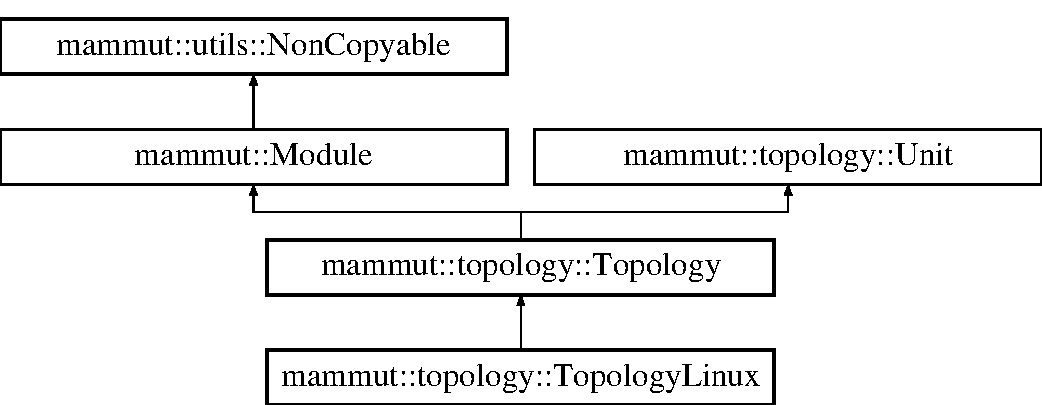
\includegraphics[height=4.000000cm]{classmammut_1_1topology_1_1TopologyLinux}
\end{center}
\end{figure}
\subsection*{Public Member Functions}
\begin{DoxyCompactItemize}
\item 
void \hyperlink{classmammut_1_1topology_1_1TopologyLinux_a9c0f603739a7e5caaed981e12c8c0937}{maximize\-Utilization} () const 
\item 
void \hyperlink{classmammut_1_1topology_1_1TopologyLinux_a8d33dfb6af9e8ec32c0501dbe7031809}{reset\-Utilization} () const 
\end{DoxyCompactItemize}
\subsection*{Additional Inherited Members}


\subsection{Member Function Documentation}
\hypertarget{classmammut_1_1topology_1_1TopologyLinux_a9c0f603739a7e5caaed981e12c8c0937}{\index{mammut\-::topology\-::\-Topology\-Linux@{mammut\-::topology\-::\-Topology\-Linux}!maximize\-Utilization@{maximize\-Utilization}}
\index{maximize\-Utilization@{maximize\-Utilization}!mammut::topology::TopologyLinux@{mammut\-::topology\-::\-Topology\-Linux}}
\subsubsection[{maximize\-Utilization}]{\setlength{\rightskip}{0pt plus 5cm}void mammut\-::topology\-::\-Topology\-Linux\-::maximize\-Utilization (
\begin{DoxyParamCaption}
{}
\end{DoxyParamCaption}
) const\hspace{0.3cm}{\ttfamily [virtual]}}}\label{classmammut_1_1topology_1_1TopologyLinux_a9c0f603739a7e5caaed981e12c8c0937}
Bring the utilization of this unit to 100\% until \hyperlink{classmammut_1_1topology_1_1TopologyLinux_a8d33dfb6af9e8ec32c0501dbe7031809}{reset\-Utilization()} is called. 

Implements \hyperlink{classmammut_1_1topology_1_1Unit_a0a12d2b5939c609c657a2bd652801e88}{mammut\-::topology\-::\-Unit}.

\hypertarget{classmammut_1_1topology_1_1TopologyLinux_a8d33dfb6af9e8ec32c0501dbe7031809}{\index{mammut\-::topology\-::\-Topology\-Linux@{mammut\-::topology\-::\-Topology\-Linux}!reset\-Utilization@{reset\-Utilization}}
\index{reset\-Utilization@{reset\-Utilization}!mammut::topology::TopologyLinux@{mammut\-::topology\-::\-Topology\-Linux}}
\subsubsection[{reset\-Utilization}]{\setlength{\rightskip}{0pt plus 5cm}void mammut\-::topology\-::\-Topology\-Linux\-::reset\-Utilization (
\begin{DoxyParamCaption}
{}
\end{DoxyParamCaption}
) const\hspace{0.3cm}{\ttfamily [virtual]}}}\label{classmammut_1_1topology_1_1TopologyLinux_a8d33dfb6af9e8ec32c0501dbe7031809}
Resets the utilization of this unit. 

Implements \hyperlink{classmammut_1_1topology_1_1Unit_a70730dde75533d3f5ecd3d3686df87cc}{mammut\-::topology\-::\-Unit}.



The documentation for this class was generated from the following files\-:\begin{DoxyCompactItemize}
\item 
/home/daniele/\-Code/\-Mammut/mammut/topology/topology-\/linux.\-hpp\item 
/home/daniele/\-Code/\-Mammut/mammut/topology/topology-\/linux.\-cpp\end{DoxyCompactItemize}

\hypertarget{classmammut_1_1topology_1_1TopologyRemote}{\section{mammut\-:\-:topology\-:\-:Topology\-Remote Class Reference}
\label{classmammut_1_1topology_1_1TopologyRemote}\index{mammut\-::topology\-::\-Topology\-Remote@{mammut\-::topology\-::\-Topology\-Remote}}
}
Inheritance diagram for mammut\-:\-:topology\-:\-:Topology\-Remote\-:\begin{figure}[H]
\begin{center}
\leavevmode
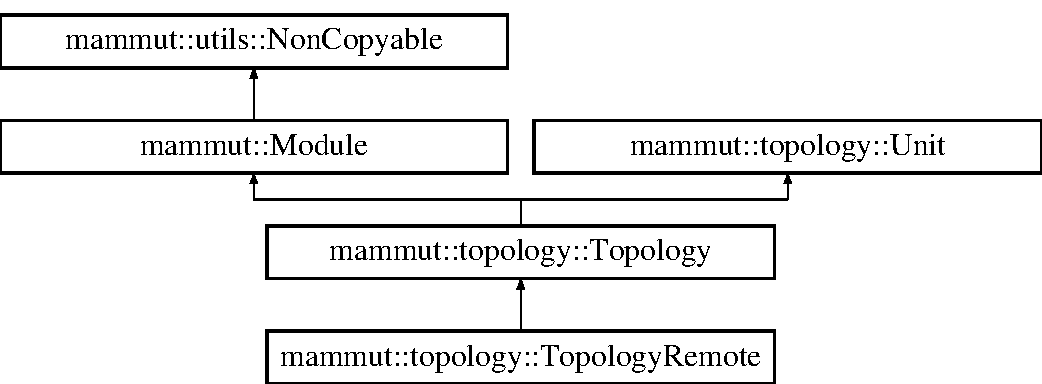
\includegraphics[height=4.000000cm]{classmammut_1_1topology_1_1TopologyRemote}
\end{center}
\end{figure}
\subsection*{Public Member Functions}
\begin{DoxyCompactItemize}
\item 
\hypertarget{classmammut_1_1topology_1_1TopologyRemote_ad08509d1104f3c0b4c5da71befc3da58}{{\bfseries Topology\-Remote} (\hyperlink{classmammut_1_1Communicator}{Communicator} $\ast$const communicator)}\label{classmammut_1_1topology_1_1TopologyRemote_ad08509d1104f3c0b4c5da71befc3da58}

\item 
void \hyperlink{classmammut_1_1topology_1_1TopologyRemote_ae5d75d4398748f79635b74fdcbe1c7f5}{maximize\-Utilization} () const 
\item 
void \hyperlink{classmammut_1_1topology_1_1TopologyRemote_a0544edb42fc7e88e23394d94929e4438}{reset\-Utilization} () const 
\end{DoxyCompactItemize}
\subsection*{Additional Inherited Members}


\subsection{Member Function Documentation}
\hypertarget{classmammut_1_1topology_1_1TopologyRemote_ae5d75d4398748f79635b74fdcbe1c7f5}{\index{mammut\-::topology\-::\-Topology\-Remote@{mammut\-::topology\-::\-Topology\-Remote}!maximize\-Utilization@{maximize\-Utilization}}
\index{maximize\-Utilization@{maximize\-Utilization}!mammut::topology::TopologyRemote@{mammut\-::topology\-::\-Topology\-Remote}}
\subsubsection[{maximize\-Utilization}]{\setlength{\rightskip}{0pt plus 5cm}void mammut\-::topology\-::\-Topology\-Remote\-::maximize\-Utilization (
\begin{DoxyParamCaption}
{}
\end{DoxyParamCaption}
) const\hspace{0.3cm}{\ttfamily [virtual]}}}\label{classmammut_1_1topology_1_1TopologyRemote_ae5d75d4398748f79635b74fdcbe1c7f5}
Bring the utilization of this unit to 100\% until \hyperlink{classmammut_1_1topology_1_1TopologyRemote_a0544edb42fc7e88e23394d94929e4438}{reset\-Utilization()} is called. 

Implements \hyperlink{classmammut_1_1topology_1_1Unit_a0a12d2b5939c609c657a2bd652801e88}{mammut\-::topology\-::\-Unit}.

\hypertarget{classmammut_1_1topology_1_1TopologyRemote_a0544edb42fc7e88e23394d94929e4438}{\index{mammut\-::topology\-::\-Topology\-Remote@{mammut\-::topology\-::\-Topology\-Remote}!reset\-Utilization@{reset\-Utilization}}
\index{reset\-Utilization@{reset\-Utilization}!mammut::topology::TopologyRemote@{mammut\-::topology\-::\-Topology\-Remote}}
\subsubsection[{reset\-Utilization}]{\setlength{\rightskip}{0pt plus 5cm}void mammut\-::topology\-::\-Topology\-Remote\-::reset\-Utilization (
\begin{DoxyParamCaption}
{}
\end{DoxyParamCaption}
) const\hspace{0.3cm}{\ttfamily [virtual]}}}\label{classmammut_1_1topology_1_1TopologyRemote_a0544edb42fc7e88e23394d94929e4438}
Resets the utilization of this unit. 

Implements \hyperlink{classmammut_1_1topology_1_1Unit_a70730dde75533d3f5ecd3d3686df87cc}{mammut\-::topology\-::\-Unit}.



The documentation for this class was generated from the following file\-:\begin{DoxyCompactItemize}
\item 
/home/daniele/\-Code/\-Mammut/mammut/topology/topology-\/remote.\-hpp\end{DoxyCompactItemize}

\hypertarget{classmammut_1_1topology_1_1Unit}{\section{mammut\-:\-:topology\-:\-:Unit Class Reference}
\label{classmammut_1_1topology_1_1Unit}\index{mammut\-::topology\-::\-Unit@{mammut\-::topology\-::\-Unit}}
}


{\ttfamily \#include $<$topology.\-hpp$>$}

Inheritance diagram for mammut\-:\-:topology\-:\-:Unit\-:\begin{figure}[H]
\begin{center}
\leavevmode
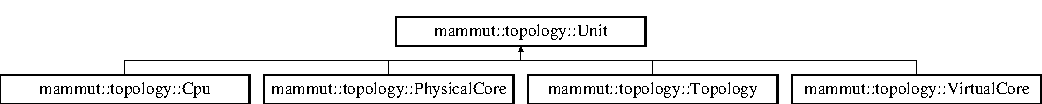
\includegraphics[height=1.161826cm]{classmammut_1_1topology_1_1Unit}
\end{center}
\end{figure}
\subsection*{Public Member Functions}
\begin{DoxyCompactItemize}
\item 
virtual void \hyperlink{classmammut_1_1topology_1_1Unit_a0a12d2b5939c609c657a2bd652801e88}{maximize\-Utilization} () const =0
\item 
virtual void \hyperlink{classmammut_1_1topology_1_1Unit_a70730dde75533d3f5ecd3d3686df87cc}{reset\-Utilization} () const =0
\end{DoxyCompactItemize}


\subsection{Detailed Description}
Generic topology unit. It may be a C\-P\-U, Physical Core or Virtual Core. 

\subsection{Member Function Documentation}
\hypertarget{classmammut_1_1topology_1_1Unit_a0a12d2b5939c609c657a2bd652801e88}{\index{mammut\-::topology\-::\-Unit@{mammut\-::topology\-::\-Unit}!maximize\-Utilization@{maximize\-Utilization}}
\index{maximize\-Utilization@{maximize\-Utilization}!mammut::topology::Unit@{mammut\-::topology\-::\-Unit}}
\subsubsection[{maximize\-Utilization}]{\setlength{\rightskip}{0pt plus 5cm}virtual void mammut\-::topology\-::\-Unit\-::maximize\-Utilization (
\begin{DoxyParamCaption}
{}
\end{DoxyParamCaption}
) const\hspace{0.3cm}{\ttfamily [pure virtual]}}}\label{classmammut_1_1topology_1_1Unit_a0a12d2b5939c609c657a2bd652801e88}
Bring the utilization of this unit to 100\% until \hyperlink{classmammut_1_1topology_1_1Unit_a70730dde75533d3f5ecd3d3686df87cc}{reset\-Utilization()} is called. 

Implemented in \hyperlink{classmammut_1_1topology_1_1VirtualCore_ac4e3a17bc401689c387f27a90e24daf5}{mammut\-::topology\-::\-Virtual\-Core}, \hyperlink{classmammut_1_1topology_1_1PhysicalCore_a2fe21bce321b3401e9108bcf29efafae}{mammut\-::topology\-::\-Physical\-Core}, \hyperlink{classmammut_1_1topology_1_1Cpu_a249829ade28b8fffcda1d2666cf68997}{mammut\-::topology\-::\-Cpu}, \hyperlink{classmammut_1_1topology_1_1VirtualCoreLinux_a9e06cca87b5879be4fe433bd409098e4}{mammut\-::topology\-::\-Virtual\-Core\-Linux}, \hyperlink{classmammut_1_1topology_1_1VirtualCoreRemote_abc026a4e9ae7db3c0d8373c520b4312d}{mammut\-::topology\-::\-Virtual\-Core\-Remote}, \hyperlink{classmammut_1_1topology_1_1PhysicalCoreRemote_ad0207a63493483caedafd82faa354c40}{mammut\-::topology\-::\-Physical\-Core\-Remote}, \hyperlink{classmammut_1_1topology_1_1PhysicalCoreLinux_a1f0d1fd02c9ac9a5960a880849affa45}{mammut\-::topology\-::\-Physical\-Core\-Linux}, \hyperlink{classmammut_1_1topology_1_1CpuLinux_a428a9356fce899f82494f0973201f009}{mammut\-::topology\-::\-Cpu\-Linux}, \hyperlink{classmammut_1_1topology_1_1CpuRemote_a1f25bdc6f2b049a831a03ba702699626}{mammut\-::topology\-::\-Cpu\-Remote}, \hyperlink{classmammut_1_1topology_1_1TopologyLinux_a9c0f603739a7e5caaed981e12c8c0937}{mammut\-::topology\-::\-Topology\-Linux}, and \hyperlink{classmammut_1_1topology_1_1TopologyRemote_ae5d75d4398748f79635b74fdcbe1c7f5}{mammut\-::topology\-::\-Topology\-Remote}.

\hypertarget{classmammut_1_1topology_1_1Unit_a70730dde75533d3f5ecd3d3686df87cc}{\index{mammut\-::topology\-::\-Unit@{mammut\-::topology\-::\-Unit}!reset\-Utilization@{reset\-Utilization}}
\index{reset\-Utilization@{reset\-Utilization}!mammut::topology::Unit@{mammut\-::topology\-::\-Unit}}
\subsubsection[{reset\-Utilization}]{\setlength{\rightskip}{0pt plus 5cm}virtual void mammut\-::topology\-::\-Unit\-::reset\-Utilization (
\begin{DoxyParamCaption}
{}
\end{DoxyParamCaption}
) const\hspace{0.3cm}{\ttfamily [pure virtual]}}}\label{classmammut_1_1topology_1_1Unit_a70730dde75533d3f5ecd3d3686df87cc}
Resets the utilization of this unit. 

Implemented in \hyperlink{classmammut_1_1topology_1_1VirtualCore_a94374b13113f0294c5178b6fc275ecc0}{mammut\-::topology\-::\-Virtual\-Core}, \hyperlink{classmammut_1_1topology_1_1PhysicalCore_ad6169b49eb4aa01fa570169735875ffe}{mammut\-::topology\-::\-Physical\-Core}, \hyperlink{classmammut_1_1topology_1_1Cpu_a3eea41d7ad6200d83301102f23944de5}{mammut\-::topology\-::\-Cpu}, \hyperlink{classmammut_1_1topology_1_1VirtualCoreLinux_a9091e0404bacb86772ee34c3c24e5713}{mammut\-::topology\-::\-Virtual\-Core\-Linux}, \hyperlink{classmammut_1_1topology_1_1VirtualCoreRemote_a43ea3102cdebec0ce6991b5638e3c4e2}{mammut\-::topology\-::\-Virtual\-Core\-Remote}, \hyperlink{classmammut_1_1topology_1_1PhysicalCoreRemote_a5f76fa7a3b9c61597ad06a2fce8db675}{mammut\-::topology\-::\-Physical\-Core\-Remote}, \hyperlink{classmammut_1_1topology_1_1PhysicalCoreLinux_a6c65161ad3041a8cedb8a9bc43757c02}{mammut\-::topology\-::\-Physical\-Core\-Linux}, \hyperlink{classmammut_1_1topology_1_1CpuLinux_ae22825c9a86f221c3ffe9c456dfe96aa}{mammut\-::topology\-::\-Cpu\-Linux}, \hyperlink{classmammut_1_1topology_1_1CpuRemote_a689af84ac46ab57081fc4fa47c9992b6}{mammut\-::topology\-::\-Cpu\-Remote}, \hyperlink{classmammut_1_1topology_1_1TopologyLinux_a8d33dfb6af9e8ec32c0501dbe7031809}{mammut\-::topology\-::\-Topology\-Linux}, and \hyperlink{classmammut_1_1topology_1_1TopologyRemote_a0544edb42fc7e88e23394d94929e4438}{mammut\-::topology\-::\-Topology\-Remote}.



The documentation for this class was generated from the following file\-:\begin{DoxyCompactItemize}
\item 
/home/daniele/\-Code/\-Mammut/mammut/topology/topology.\-hpp\end{DoxyCompactItemize}

\hypertarget{classmammut_1_1topology_1_1VirtualCore}{\section{mammut\-:\-:topology\-:\-:Virtual\-Core Class Reference}
\label{classmammut_1_1topology_1_1VirtualCore}\index{mammut\-::topology\-::\-Virtual\-Core@{mammut\-::topology\-::\-Virtual\-Core}}
}
Inheritance diagram for mammut\-:\-:topology\-:\-:Virtual\-Core\-:\begin{figure}[H]
\begin{center}
\leavevmode
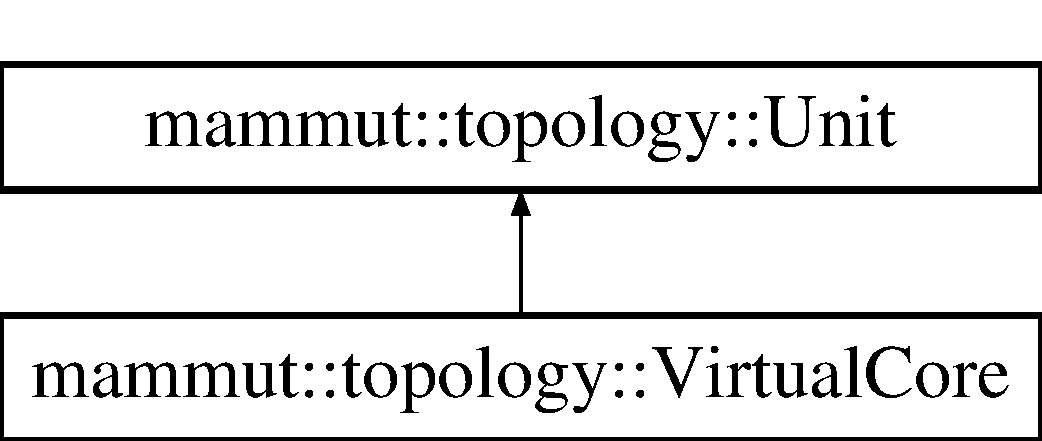
\includegraphics[height=2.000000cm]{classmammut_1_1topology_1_1VirtualCore}
\end{center}
\end{figure}
\subsection*{Public Member Functions}
\begin{DoxyCompactItemize}
\item 
Virtual\-Core\-Id \hyperlink{classmammut_1_1topology_1_1VirtualCore_ae9b5118e3e28805d4d9b3429d1b215a7}{get\-Virtual\-Core\-Id} () const 
\item 
Physical\-Core\-Id \hyperlink{classmammut_1_1topology_1_1VirtualCore_a2af7ef4acf15330f86050c2aff354a71}{get\-Physical\-Core\-Id} () const 
\item 
Cpu\-Id \hyperlink{classmammut_1_1topology_1_1VirtualCore_aa2c26a312e610dd2f6e9aa8fbcd35223}{get\-Cpu\-Id} () const 
\item 
virtual bool \hyperlink{classmammut_1_1topology_1_1VirtualCore_aa9f4400708c97197f66bcd11aa0eb990}{has\-Flag} (const std\-::string \&flag\-Name) const =0
\item 
virtual uint64\-\_\-t \hyperlink{classmammut_1_1topology_1_1VirtualCore_a0b1ac9c138d1ed5e8eceb38e619e1e65}{get\-Absolute\-Ticks} () const =0
\item 
virtual bool \hyperlink{classmammut_1_1topology_1_1VirtualCore_a545414bb4933faeba1f071e8a2ed4202}{are\-Ticks\-Constant} () const 
\item 
virtual void \hyperlink{classmammut_1_1topology_1_1VirtualCore_ac4e3a17bc401689c387f27a90e24daf5}{maximize\-Utilization} () const =0
\item 
virtual void \hyperlink{classmammut_1_1topology_1_1VirtualCore_a94374b13113f0294c5178b6fc275ecc0}{reset\-Utilization} () const =0
\item 
virtual double \hyperlink{classmammut_1_1topology_1_1VirtualCore_ad4a33cf2323e7b05537485e4b08a4f12}{get\-Idle\-Time} () const =0
\item 
virtual void \hyperlink{classmammut_1_1topology_1_1VirtualCore_a8fc6a3a4882ca369e37a3a9f0f668d9c}{reset\-Idle\-Time} ()=0
\item 
virtual bool \hyperlink{classmammut_1_1topology_1_1VirtualCore_ab8eb88bee673244367a5394de87142d5}{is\-Hot\-Pluggable} () const =0
\item 
virtual bool \hyperlink{classmammut_1_1topology_1_1VirtualCore_a61bd18dbc9bd35f6b22e9bbd7947427d}{is\-Hot\-Plugged} () const =0
\item 
virtual void \hyperlink{classmammut_1_1topology_1_1VirtualCore_a7674d352e60bb8d9c183ca54f62b383d}{hot\-Plug} () const =0
\item 
virtual void \hyperlink{classmammut_1_1topology_1_1VirtualCore_a1e8ce49fd0885331533fa85ad7504a9d}{hot\-Unplug} () const =0
\item 
virtual std\-::vector\\*
$<$ \hyperlink{classmammut_1_1topology_1_1VirtualCoreIdleLevel}{Virtual\-Core\-Idle\-Level} $\ast$ $>$ \hyperlink{classmammut_1_1topology_1_1VirtualCore_a841dd64b1b74b28a0533cc1aa9d8cb84}{get\-Idle\-Levels} () const =0
\end{DoxyCompactItemize}
\subsection*{Protected Member Functions}
\begin{DoxyCompactItemize}
\item 
\hypertarget{classmammut_1_1topology_1_1VirtualCore_ae30b9c960484969abc9b7ea8807a7e40}{{\bfseries Virtual\-Core} (Cpu\-Id cpu\-Id, Physical\-Core\-Id physical\-Core\-Id, Virtual\-Core\-Id virtual\-Core\-Id)}\label{classmammut_1_1topology_1_1VirtualCore_ae30b9c960484969abc9b7ea8807a7e40}

\end{DoxyCompactItemize}
\subsection*{Protected Attributes}
\begin{DoxyCompactItemize}
\item 
\hypertarget{classmammut_1_1topology_1_1VirtualCore_a34b200cab13ee901ea5a8b9fcc17e81a}{const Cpu\-Id {\bfseries \-\_\-cpu\-Id}}\label{classmammut_1_1topology_1_1VirtualCore_a34b200cab13ee901ea5a8b9fcc17e81a}

\item 
\hypertarget{classmammut_1_1topology_1_1VirtualCore_a9dd71de7005506fb5631891ce0144b94}{const Physical\-Core\-Id {\bfseries \-\_\-physical\-Core\-Id}}\label{classmammut_1_1topology_1_1VirtualCore_a9dd71de7005506fb5631891ce0144b94}

\item 
\hypertarget{classmammut_1_1topology_1_1VirtualCore_a86acd2c039f8d9cfde1ef3c0a58a6232}{const Virtual\-Core\-Id {\bfseries \-\_\-virtual\-Core\-Id}}\label{classmammut_1_1topology_1_1VirtualCore_a86acd2c039f8d9cfde1ef3c0a58a6232}

\end{DoxyCompactItemize}


\subsection{Member Function Documentation}
\hypertarget{classmammut_1_1topology_1_1VirtualCore_a545414bb4933faeba1f071e8a2ed4202}{\index{mammut\-::topology\-::\-Virtual\-Core@{mammut\-::topology\-::\-Virtual\-Core}!are\-Ticks\-Constant@{are\-Ticks\-Constant}}
\index{are\-Ticks\-Constant@{are\-Ticks\-Constant}!mammut::topology::VirtualCore@{mammut\-::topology\-::\-Virtual\-Core}}
\subsubsection[{are\-Ticks\-Constant}]{\setlength{\rightskip}{0pt plus 5cm}virtual bool mammut\-::topology\-::\-Virtual\-Core\-::are\-Ticks\-Constant (
\begin{DoxyParamCaption}
{}
\end{DoxyParamCaption}
) const\hspace{0.3cm}{\ttfamily [virtual]}}}\label{classmammut_1_1topology_1_1VirtualCore_a545414bb4933faeba1f071e8a2ed4202}
Check if the amount of ticks per second change with frequency. \begin{DoxyReturn}{Returns}
True if ticks do not change with frequency, false otherwise. 
\end{DoxyReturn}
\hypertarget{classmammut_1_1topology_1_1VirtualCore_a0b1ac9c138d1ed5e8eceb38e619e1e65}{\index{mammut\-::topology\-::\-Virtual\-Core@{mammut\-::topology\-::\-Virtual\-Core}!get\-Absolute\-Ticks@{get\-Absolute\-Ticks}}
\index{get\-Absolute\-Ticks@{get\-Absolute\-Ticks}!mammut::topology::VirtualCore@{mammut\-::topology\-::\-Virtual\-Core}}
\subsubsection[{get\-Absolute\-Ticks}]{\setlength{\rightskip}{0pt plus 5cm}virtual uint64\-\_\-t mammut\-::topology\-::\-Virtual\-Core\-::get\-Absolute\-Ticks (
\begin{DoxyParamCaption}
{}
\end{DoxyParamCaption}
) const\hspace{0.3cm}{\ttfamily [pure virtual]}}}\label{classmammut_1_1topology_1_1VirtualCore_a0b1ac9c138d1ed5e8eceb38e619e1e65}
Gets the clock ticks of this virtual core. \begin{DoxyReturn}{Returns}
The clock ticks of this virtual core. If 0 is returned, ticks are not available. A\-T\-T\-E\-N\-T\-I\-O\-N\-: In general, ticks may change with frequency, i.\-e. the amount of ticks per second at 1\-G\-Hz may be different from the amount of ticks per second at 2\-G\-Hz. To check if ticks do not change with the frequency, you should use '\hyperlink{classmammut_1_1topology_1_1VirtualCore_a545414bb4933faeba1f071e8a2ed4202}{are\-Ticks\-Constant()}' call. 
\end{DoxyReturn}
\hypertarget{classmammut_1_1topology_1_1VirtualCore_aa2c26a312e610dd2f6e9aa8fbcd35223}{\index{mammut\-::topology\-::\-Virtual\-Core@{mammut\-::topology\-::\-Virtual\-Core}!get\-Cpu\-Id@{get\-Cpu\-Id}}
\index{get\-Cpu\-Id@{get\-Cpu\-Id}!mammut::topology::VirtualCore@{mammut\-::topology\-::\-Virtual\-Core}}
\subsubsection[{get\-Cpu\-Id}]{\setlength{\rightskip}{0pt plus 5cm}Cpu\-Id mammut\-::topology\-::\-Virtual\-Core\-::get\-Cpu\-Id (
\begin{DoxyParamCaption}
{}
\end{DoxyParamCaption}
) const}}\label{classmammut_1_1topology_1_1VirtualCore_aa2c26a312e610dd2f6e9aa8fbcd35223}
Returns the identifier of the C\-P\-U on which this virtual core is running. \begin{DoxyReturn}{Returns}
The identifier of the C\-P\-U on which this virtual core is running. 
\end{DoxyReturn}
\hypertarget{classmammut_1_1topology_1_1VirtualCore_a841dd64b1b74b28a0533cc1aa9d8cb84}{\index{mammut\-::topology\-::\-Virtual\-Core@{mammut\-::topology\-::\-Virtual\-Core}!get\-Idle\-Levels@{get\-Idle\-Levels}}
\index{get\-Idle\-Levels@{get\-Idle\-Levels}!mammut::topology::VirtualCore@{mammut\-::topology\-::\-Virtual\-Core}}
\subsubsection[{get\-Idle\-Levels}]{\setlength{\rightskip}{0pt plus 5cm}virtual std\-::vector$<${\bf Virtual\-Core\-Idle\-Level}$\ast$$>$ mammut\-::topology\-::\-Virtual\-Core\-::get\-Idle\-Levels (
\begin{DoxyParamCaption}
{}
\end{DoxyParamCaption}
) const\hspace{0.3cm}{\ttfamily [pure virtual]}}}\label{classmammut_1_1topology_1_1VirtualCore_a841dd64b1b74b28a0533cc1aa9d8cb84}
Returns the idle levels (C-\/\-States) supported by this virtual core. \begin{DoxyReturn}{Returns}
The idle levels supported by this virtual core. If the vector is empty, no idle levels are supported. 
\end{DoxyReturn}
\hypertarget{classmammut_1_1topology_1_1VirtualCore_ad4a33cf2323e7b05537485e4b08a4f12}{\index{mammut\-::topology\-::\-Virtual\-Core@{mammut\-::topology\-::\-Virtual\-Core}!get\-Idle\-Time@{get\-Idle\-Time}}
\index{get\-Idle\-Time@{get\-Idle\-Time}!mammut::topology::VirtualCore@{mammut\-::topology\-::\-Virtual\-Core}}
\subsubsection[{get\-Idle\-Time}]{\setlength{\rightskip}{0pt plus 5cm}virtual double mammut\-::topology\-::\-Virtual\-Core\-::get\-Idle\-Time (
\begin{DoxyParamCaption}
{}
\end{DoxyParamCaption}
) const\hspace{0.3cm}{\ttfamily [pure virtual]}}}\label{classmammut_1_1topology_1_1VirtualCore_ad4a33cf2323e7b05537485e4b08a4f12}
Returns the number of microseconds that this virtual core have been idle since the last call of \hyperlink{classmammut_1_1topology_1_1VirtualCore_a8fc6a3a4882ca369e37a3a9f0f668d9c}{reset\-Idle\-Time()} (or since the creation of this virtual core handler). \begin{DoxyReturn}{Returns}
The number of microseconds that this virtual core have been idle. 
\end{DoxyReturn}
\hypertarget{classmammut_1_1topology_1_1VirtualCore_a2af7ef4acf15330f86050c2aff354a71}{\index{mammut\-::topology\-::\-Virtual\-Core@{mammut\-::topology\-::\-Virtual\-Core}!get\-Physical\-Core\-Id@{get\-Physical\-Core\-Id}}
\index{get\-Physical\-Core\-Id@{get\-Physical\-Core\-Id}!mammut::topology::VirtualCore@{mammut\-::topology\-::\-Virtual\-Core}}
\subsubsection[{get\-Physical\-Core\-Id}]{\setlength{\rightskip}{0pt plus 5cm}Physical\-Core\-Id mammut\-::topology\-::\-Virtual\-Core\-::get\-Physical\-Core\-Id (
\begin{DoxyParamCaption}
{}
\end{DoxyParamCaption}
) const}}\label{classmammut_1_1topology_1_1VirtualCore_a2af7ef4acf15330f86050c2aff354a71}
Returns the identifier of the physical core on which this virtual core is running. \begin{DoxyReturn}{Returns}
The identifier of the physical core on which this virtual core is running. 
\end{DoxyReturn}
\hypertarget{classmammut_1_1topology_1_1VirtualCore_ae9b5118e3e28805d4d9b3429d1b215a7}{\index{mammut\-::topology\-::\-Virtual\-Core@{mammut\-::topology\-::\-Virtual\-Core}!get\-Virtual\-Core\-Id@{get\-Virtual\-Core\-Id}}
\index{get\-Virtual\-Core\-Id@{get\-Virtual\-Core\-Id}!mammut::topology::VirtualCore@{mammut\-::topology\-::\-Virtual\-Core}}
\subsubsection[{get\-Virtual\-Core\-Id}]{\setlength{\rightskip}{0pt plus 5cm}Virtual\-Core\-Id mammut\-::topology\-::\-Virtual\-Core\-::get\-Virtual\-Core\-Id (
\begin{DoxyParamCaption}
{}
\end{DoxyParamCaption}
) const}}\label{classmammut_1_1topology_1_1VirtualCore_ae9b5118e3e28805d4d9b3429d1b215a7}
Returns the identifier of this virtual core. \begin{DoxyReturn}{Returns}
The identifier of this virtual core. 
\end{DoxyReturn}
\hypertarget{classmammut_1_1topology_1_1VirtualCore_aa9f4400708c97197f66bcd11aa0eb990}{\index{mammut\-::topology\-::\-Virtual\-Core@{mammut\-::topology\-::\-Virtual\-Core}!has\-Flag@{has\-Flag}}
\index{has\-Flag@{has\-Flag}!mammut::topology::VirtualCore@{mammut\-::topology\-::\-Virtual\-Core}}
\subsubsection[{has\-Flag}]{\setlength{\rightskip}{0pt plus 5cm}virtual bool mammut\-::topology\-::\-Virtual\-Core\-::has\-Flag (
\begin{DoxyParamCaption}
\item[{const std\-::string \&}]{flag\-Name}
\end{DoxyParamCaption}
) const\hspace{0.3cm}{\ttfamily [pure virtual]}}}\label{classmammut_1_1topology_1_1VirtualCore_aa9f4400708c97197f66bcd11aa0eb990}
Checks if this virtual core has a specific flag \hypertarget{classmammut_1_1topology_1_1VirtualCore_a7674d352e60bb8d9c183ca54f62b383d}{\index{mammut\-::topology\-::\-Virtual\-Core@{mammut\-::topology\-::\-Virtual\-Core}!hot\-Plug@{hot\-Plug}}
\index{hot\-Plug@{hot\-Plug}!mammut::topology::VirtualCore@{mammut\-::topology\-::\-Virtual\-Core}}
\subsubsection[{hot\-Plug}]{\setlength{\rightskip}{0pt plus 5cm}virtual void mammut\-::topology\-::\-Virtual\-Core\-::hot\-Plug (
\begin{DoxyParamCaption}
{}
\end{DoxyParamCaption}
) const\hspace{0.3cm}{\ttfamily [pure virtual]}}}\label{classmammut_1_1topology_1_1VirtualCore_a7674d352e60bb8d9c183ca54f62b383d}
Hotplugs this virtual core. If this core is not hot-\/pluggable, nothing is done. \hypertarget{classmammut_1_1topology_1_1VirtualCore_a1e8ce49fd0885331533fa85ad7504a9d}{\index{mammut\-::topology\-::\-Virtual\-Core@{mammut\-::topology\-::\-Virtual\-Core}!hot\-Unplug@{hot\-Unplug}}
\index{hot\-Unplug@{hot\-Unplug}!mammut::topology::VirtualCore@{mammut\-::topology\-::\-Virtual\-Core}}
\subsubsection[{hot\-Unplug}]{\setlength{\rightskip}{0pt plus 5cm}virtual void mammut\-::topology\-::\-Virtual\-Core\-::hot\-Unplug (
\begin{DoxyParamCaption}
{}
\end{DoxyParamCaption}
) const\hspace{0.3cm}{\ttfamily [pure virtual]}}}\label{classmammut_1_1topology_1_1VirtualCore_a1e8ce49fd0885331533fa85ad7504a9d}
Hotunplugs this virtual core. If this core is not hot-\/pluggable, nothing is done. \hypertarget{classmammut_1_1topology_1_1VirtualCore_ab8eb88bee673244367a5394de87142d5}{\index{mammut\-::topology\-::\-Virtual\-Core@{mammut\-::topology\-::\-Virtual\-Core}!is\-Hot\-Pluggable@{is\-Hot\-Pluggable}}
\index{is\-Hot\-Pluggable@{is\-Hot\-Pluggable}!mammut::topology::VirtualCore@{mammut\-::topology\-::\-Virtual\-Core}}
\subsubsection[{is\-Hot\-Pluggable}]{\setlength{\rightskip}{0pt plus 5cm}virtual bool mammut\-::topology\-::\-Virtual\-Core\-::is\-Hot\-Pluggable (
\begin{DoxyParamCaption}
{}
\end{DoxyParamCaption}
) const\hspace{0.3cm}{\ttfamily [pure virtual]}}}\label{classmammut_1_1topology_1_1VirtualCore_ab8eb88bee673244367a5394de87142d5}
Returns true if this virtual core is hot-\/pluggable. \begin{DoxyReturn}{Returns}
True if this virtual core is hot-\/pluggable, false otherwise. 
\end{DoxyReturn}
\hypertarget{classmammut_1_1topology_1_1VirtualCore_a61bd18dbc9bd35f6b22e9bbd7947427d}{\index{mammut\-::topology\-::\-Virtual\-Core@{mammut\-::topology\-::\-Virtual\-Core}!is\-Hot\-Plugged@{is\-Hot\-Plugged}}
\index{is\-Hot\-Plugged@{is\-Hot\-Plugged}!mammut::topology::VirtualCore@{mammut\-::topology\-::\-Virtual\-Core}}
\subsubsection[{is\-Hot\-Plugged}]{\setlength{\rightskip}{0pt plus 5cm}virtual bool mammut\-::topology\-::\-Virtual\-Core\-::is\-Hot\-Plugged (
\begin{DoxyParamCaption}
{}
\end{DoxyParamCaption}
) const\hspace{0.3cm}{\ttfamily [pure virtual]}}}\label{classmammut_1_1topology_1_1VirtualCore_a61bd18dbc9bd35f6b22e9bbd7947427d}
Returns true if this virtual core is hot plugged. \begin{DoxyReturn}{Returns}
True if this virtual core is hot plugged or if hotplug is not supported, false otherwise. 
\end{DoxyReturn}
\hypertarget{classmammut_1_1topology_1_1VirtualCore_ac4e3a17bc401689c387f27a90e24daf5}{\index{mammut\-::topology\-::\-Virtual\-Core@{mammut\-::topology\-::\-Virtual\-Core}!maximize\-Utilization@{maximize\-Utilization}}
\index{maximize\-Utilization@{maximize\-Utilization}!mammut::topology::VirtualCore@{mammut\-::topology\-::\-Virtual\-Core}}
\subsubsection[{maximize\-Utilization}]{\setlength{\rightskip}{0pt plus 5cm}virtual void mammut\-::topology\-::\-Virtual\-Core\-::maximize\-Utilization (
\begin{DoxyParamCaption}
{}
\end{DoxyParamCaption}
) const\hspace{0.3cm}{\ttfamily [pure virtual]}}}\label{classmammut_1_1topology_1_1VirtualCore_ac4e3a17bc401689c387f27a90e24daf5}
Bring the utilization of this virtual core to 100\% until \hyperlink{classmammut_1_1topology_1_1VirtualCore_a94374b13113f0294c5178b6fc275ecc0}{reset\-Utilization()} is called. 

Implements \hyperlink{classmammut_1_1topology_1_1Unit_a0a12d2b5939c609c657a2bd652801e88}{mammut\-::topology\-::\-Unit}.

\hypertarget{classmammut_1_1topology_1_1VirtualCore_a8fc6a3a4882ca369e37a3a9f0f668d9c}{\index{mammut\-::topology\-::\-Virtual\-Core@{mammut\-::topology\-::\-Virtual\-Core}!reset\-Idle\-Time@{reset\-Idle\-Time}}
\index{reset\-Idle\-Time@{reset\-Idle\-Time}!mammut::topology::VirtualCore@{mammut\-::topology\-::\-Virtual\-Core}}
\subsubsection[{reset\-Idle\-Time}]{\setlength{\rightskip}{0pt plus 5cm}virtual void mammut\-::topology\-::\-Virtual\-Core\-::reset\-Idle\-Time (
\begin{DoxyParamCaption}
{}
\end{DoxyParamCaption}
)\hspace{0.3cm}{\ttfamily [pure virtual]}}}\label{classmammut_1_1topology_1_1VirtualCore_a8fc6a3a4882ca369e37a3a9f0f668d9c}
Resets the number of microseconds that this virtual core have been idle \hypertarget{classmammut_1_1topology_1_1VirtualCore_a94374b13113f0294c5178b6fc275ecc0}{\index{mammut\-::topology\-::\-Virtual\-Core@{mammut\-::topology\-::\-Virtual\-Core}!reset\-Utilization@{reset\-Utilization}}
\index{reset\-Utilization@{reset\-Utilization}!mammut::topology::VirtualCore@{mammut\-::topology\-::\-Virtual\-Core}}
\subsubsection[{reset\-Utilization}]{\setlength{\rightskip}{0pt plus 5cm}virtual void mammut\-::topology\-::\-Virtual\-Core\-::reset\-Utilization (
\begin{DoxyParamCaption}
{}
\end{DoxyParamCaption}
) const\hspace{0.3cm}{\ttfamily [pure virtual]}}}\label{classmammut_1_1topology_1_1VirtualCore_a94374b13113f0294c5178b6fc275ecc0}
Resets the utilization of this virtual core. 

Implements \hyperlink{classmammut_1_1topology_1_1Unit_a70730dde75533d3f5ecd3d3686df87cc}{mammut\-::topology\-::\-Unit}.



The documentation for this class was generated from the following file\-:\begin{DoxyCompactItemize}
\item 
/home/daniele/\-Code/\-Mammut/mammut/topology/topology.\-hpp\end{DoxyCompactItemize}

\hypertarget{structmammut_1_1topology_1_1VirtualCoreCoordinates}{\section{mammut\-:\-:topology\-:\-:Virtual\-Core\-Coordinates Struct Reference}
\label{structmammut_1_1topology_1_1VirtualCoreCoordinates}\index{mammut\-::topology\-::\-Virtual\-Core\-Coordinates@{mammut\-::topology\-::\-Virtual\-Core\-Coordinates}}
}
\subsection*{Public Attributes}
\begin{DoxyCompactItemize}
\item 
\hypertarget{structmammut_1_1topology_1_1VirtualCoreCoordinates_af040bfac88a5f4ac6e3e7df9a316b9e9}{Cpu\-Id {\bfseries cpu\-Id}}\label{structmammut_1_1topology_1_1VirtualCoreCoordinates_af040bfac88a5f4ac6e3e7df9a316b9e9}

\item 
\hypertarget{structmammut_1_1topology_1_1VirtualCoreCoordinates_ad1029daa743f9288dd54a7de26e2b501}{Physical\-Core\-Id {\bfseries physical\-Core\-Id}}\label{structmammut_1_1topology_1_1VirtualCoreCoordinates_ad1029daa743f9288dd54a7de26e2b501}

\item 
\hypertarget{structmammut_1_1topology_1_1VirtualCoreCoordinates_a9e39fa2bd3806f1b6edcf092f9b14bc2}{Virtual\-Core\-Id {\bfseries virtual\-Core\-Id}}\label{structmammut_1_1topology_1_1VirtualCoreCoordinates_a9e39fa2bd3806f1b6edcf092f9b14bc2}

\end{DoxyCompactItemize}


The documentation for this struct was generated from the following file\-:\begin{DoxyCompactItemize}
\item 
/home/daniele/\-Code/\-Mammut/mammut/topology/topology.\-hpp\end{DoxyCompactItemize}

\hypertarget{classmammut_1_1topology_1_1VirtualCoreIdleLevel}{\section{mammut\-:\-:topology\-:\-:Virtual\-Core\-Idle\-Level Class Reference}
\label{classmammut_1_1topology_1_1VirtualCoreIdleLevel}\index{mammut\-::topology\-::\-Virtual\-Core\-Idle\-Level@{mammut\-::topology\-::\-Virtual\-Core\-Idle\-Level}}
}
\subsection*{Public Member Functions}
\begin{DoxyCompactItemize}
\item 
Virtual\-Core\-Id \hyperlink{classmammut_1_1topology_1_1VirtualCoreIdleLevel_a1145d3ff6d9052589afc4b308896e789}{get\-Virtual\-Core\-Id} () const 
\item 
uint \hyperlink{classmammut_1_1topology_1_1VirtualCoreIdleLevel_a0b3c6dc7b77dedb33753c751f59b3b42}{get\-Level\-Id} () const 
\item 
virtual std\-::string \hyperlink{classmammut_1_1topology_1_1VirtualCoreIdleLevel_a0e11b685cd38c09e4e6fd7610670ffd5}{get\-Name} () const =0
\item 
virtual std\-::string \hyperlink{classmammut_1_1topology_1_1VirtualCoreIdleLevel_af2542933dbfe7e83ff9c522a43d96d45}{get\-Desc} () const =0
\item 
virtual bool \hyperlink{classmammut_1_1topology_1_1VirtualCoreIdleLevel_afac261b8838df4df7f694dab365643d2}{is\-Enableable} () const =0
\item 
virtual bool \hyperlink{classmammut_1_1topology_1_1VirtualCoreIdleLevel_acabc887668492f3e085aae5bb905558a}{is\-Enabled} () const =0
\item 
virtual void \hyperlink{classmammut_1_1topology_1_1VirtualCoreIdleLevel_aac5bccbd57ef3246ac6c268204a337ab}{enable} () const =0
\item 
virtual void \hyperlink{classmammut_1_1topology_1_1VirtualCoreIdleLevel_a25ce6958cae064d55055c7940d236f9d}{disable} () const =0
\item 
virtual uint \hyperlink{classmammut_1_1topology_1_1VirtualCoreIdleLevel_ab4ab28cce2c5b0d46b94cb0bae02bba5}{get\-Exit\-Latency} () const =0
\item 
virtual uint \hyperlink{classmammut_1_1topology_1_1VirtualCoreIdleLevel_a0be5f6e317cbfeb8825a21f13ae3e78d}{get\-Consumed\-Power} () const =0
\item 
virtual uint \hyperlink{classmammut_1_1topology_1_1VirtualCoreIdleLevel_ae841eaa71ad7accb31c37f06f6479030}{get\-Absolute\-Time} () const =0
\item 
virtual uint \hyperlink{classmammut_1_1topology_1_1VirtualCoreIdleLevel_a44854d4cd60b782ae2738fff8e86ca6e}{get\-Time} () const =0
\item 
virtual void \hyperlink{classmammut_1_1topology_1_1VirtualCoreIdleLevel_a22fff5c84d8b377fa1845cafd0df0112}{reset\-Time} ()=0
\item 
virtual uint \hyperlink{classmammut_1_1topology_1_1VirtualCoreIdleLevel_a77b2e87e91dedf6dfa593324875c94fa}{get\-Absolute\-Count} () const =0
\item 
virtual uint \hyperlink{classmammut_1_1topology_1_1VirtualCoreIdleLevel_a031d27afe2c4a164f35fc2c2eeaa22ca}{get\-Count} () const =0
\item 
virtual void \hyperlink{classmammut_1_1topology_1_1VirtualCoreIdleLevel_adf46930dfd0fc152490405f586394fd3}{reset\-Count} ()=0
\end{DoxyCompactItemize}
\subsection*{Protected Member Functions}
\begin{DoxyCompactItemize}
\item 
\hypertarget{classmammut_1_1topology_1_1VirtualCoreIdleLevel_aaa9ecf7f95a81177ab03db5362b5af02}{{\bfseries Virtual\-Core\-Idle\-Level} (Virtual\-Core\-Id virtual\-Core\-Id, uint level\-Id)}\label{classmammut_1_1topology_1_1VirtualCoreIdleLevel_aaa9ecf7f95a81177ab03db5362b5af02}

\end{DoxyCompactItemize}
\subsection*{Protected Attributes}
\begin{DoxyCompactItemize}
\item 
\hypertarget{classmammut_1_1topology_1_1VirtualCoreIdleLevel_a04232f0908e795991f658e6ef271315f}{const Virtual\-Core\-Id {\bfseries \-\_\-virtual\-Core\-Id}}\label{classmammut_1_1topology_1_1VirtualCoreIdleLevel_a04232f0908e795991f658e6ef271315f}

\item 
\hypertarget{classmammut_1_1topology_1_1VirtualCoreIdleLevel_a23b0cb5c7f06c62d5b7f98e52186aac1}{const uint {\bfseries \-\_\-level\-Id}}\label{classmammut_1_1topology_1_1VirtualCoreIdleLevel_a23b0cb5c7f06c62d5b7f98e52186aac1}

\end{DoxyCompactItemize}


\subsection{Member Function Documentation}
\hypertarget{classmammut_1_1topology_1_1VirtualCoreIdleLevel_a25ce6958cae064d55055c7940d236f9d}{\index{mammut\-::topology\-::\-Virtual\-Core\-Idle\-Level@{mammut\-::topology\-::\-Virtual\-Core\-Idle\-Level}!disable@{disable}}
\index{disable@{disable}!mammut::topology::VirtualCoreIdleLevel@{mammut\-::topology\-::\-Virtual\-Core\-Idle\-Level}}
\subsubsection[{disable}]{\setlength{\rightskip}{0pt plus 5cm}virtual void mammut\-::topology\-::\-Virtual\-Core\-Idle\-Level\-::disable (
\begin{DoxyParamCaption}
{}
\end{DoxyParamCaption}
) const\hspace{0.3cm}{\ttfamily [pure virtual]}}}\label{classmammut_1_1topology_1_1VirtualCoreIdleLevel_a25ce6958cae064d55055c7940d236f9d}
Disables this level. \hypertarget{classmammut_1_1topology_1_1VirtualCoreIdleLevel_aac5bccbd57ef3246ac6c268204a337ab}{\index{mammut\-::topology\-::\-Virtual\-Core\-Idle\-Level@{mammut\-::topology\-::\-Virtual\-Core\-Idle\-Level}!enable@{enable}}
\index{enable@{enable}!mammut::topology::VirtualCoreIdleLevel@{mammut\-::topology\-::\-Virtual\-Core\-Idle\-Level}}
\subsubsection[{enable}]{\setlength{\rightskip}{0pt plus 5cm}virtual void mammut\-::topology\-::\-Virtual\-Core\-Idle\-Level\-::enable (
\begin{DoxyParamCaption}
{}
\end{DoxyParamCaption}
) const\hspace{0.3cm}{\ttfamily [pure virtual]}}}\label{classmammut_1_1topology_1_1VirtualCoreIdleLevel_aac5bccbd57ef3246ac6c268204a337ab}
Enables this level. \hypertarget{classmammut_1_1topology_1_1VirtualCoreIdleLevel_a77b2e87e91dedf6dfa593324875c94fa}{\index{mammut\-::topology\-::\-Virtual\-Core\-Idle\-Level@{mammut\-::topology\-::\-Virtual\-Core\-Idle\-Level}!get\-Absolute\-Count@{get\-Absolute\-Count}}
\index{get\-Absolute\-Count@{get\-Absolute\-Count}!mammut::topology::VirtualCoreIdleLevel@{mammut\-::topology\-::\-Virtual\-Core\-Idle\-Level}}
\subsubsection[{get\-Absolute\-Count}]{\setlength{\rightskip}{0pt plus 5cm}virtual uint mammut\-::topology\-::\-Virtual\-Core\-Idle\-Level\-::get\-Absolute\-Count (
\begin{DoxyParamCaption}
{}
\end{DoxyParamCaption}
) const\hspace{0.3cm}{\ttfamily [pure virtual]}}}\label{classmammut_1_1topology_1_1VirtualCoreIdleLevel_a77b2e87e91dedf6dfa593324875c94fa}
Returns the number of times this level was entered. It is updated only when there is a level change. Accordingly, it could be inaccurate. \begin{DoxyReturn}{Returns}
The number of times this level was entered. 
\end{DoxyReturn}
\hypertarget{classmammut_1_1topology_1_1VirtualCoreIdleLevel_ae841eaa71ad7accb31c37f06f6479030}{\index{mammut\-::topology\-::\-Virtual\-Core\-Idle\-Level@{mammut\-::topology\-::\-Virtual\-Core\-Idle\-Level}!get\-Absolute\-Time@{get\-Absolute\-Time}}
\index{get\-Absolute\-Time@{get\-Absolute\-Time}!mammut::topology::VirtualCoreIdleLevel@{mammut\-::topology\-::\-Virtual\-Core\-Idle\-Level}}
\subsubsection[{get\-Absolute\-Time}]{\setlength{\rightskip}{0pt plus 5cm}virtual uint mammut\-::topology\-::\-Virtual\-Core\-Idle\-Level\-::get\-Absolute\-Time (
\begin{DoxyParamCaption}
{}
\end{DoxyParamCaption}
) const\hspace{0.3cm}{\ttfamily [pure virtual]}}}\label{classmammut_1_1topology_1_1VirtualCoreIdleLevel_ae841eaa71ad7accb31c37f06f6479030}
Returns the total time spent in this level (in microseconds). It is updated only when there is a level change. Accordingly, it could be inaccurate. \begin{DoxyReturn}{Returns}
The total time spent in this level (in microseconds). 
\end{DoxyReturn}
\hypertarget{classmammut_1_1topology_1_1VirtualCoreIdleLevel_a0be5f6e317cbfeb8825a21f13ae3e78d}{\index{mammut\-::topology\-::\-Virtual\-Core\-Idle\-Level@{mammut\-::topology\-::\-Virtual\-Core\-Idle\-Level}!get\-Consumed\-Power@{get\-Consumed\-Power}}
\index{get\-Consumed\-Power@{get\-Consumed\-Power}!mammut::topology::VirtualCoreIdleLevel@{mammut\-::topology\-::\-Virtual\-Core\-Idle\-Level}}
\subsubsection[{get\-Consumed\-Power}]{\setlength{\rightskip}{0pt plus 5cm}virtual uint mammut\-::topology\-::\-Virtual\-Core\-Idle\-Level\-::get\-Consumed\-Power (
\begin{DoxyParamCaption}
{}
\end{DoxyParamCaption}
) const\hspace{0.3cm}{\ttfamily [pure virtual]}}}\label{classmammut_1_1topology_1_1VirtualCoreIdleLevel_a0be5f6e317cbfeb8825a21f13ae3e78d}
Returns the power consumed while in this level (in milliwatts). \begin{DoxyReturn}{Returns}
The power consumed while in this level (in milliwatts). 
\end{DoxyReturn}
\hypertarget{classmammut_1_1topology_1_1VirtualCoreIdleLevel_a031d27afe2c4a164f35fc2c2eeaa22ca}{\index{mammut\-::topology\-::\-Virtual\-Core\-Idle\-Level@{mammut\-::topology\-::\-Virtual\-Core\-Idle\-Level}!get\-Count@{get\-Count}}
\index{get\-Count@{get\-Count}!mammut::topology::VirtualCoreIdleLevel@{mammut\-::topology\-::\-Virtual\-Core\-Idle\-Level}}
\subsubsection[{get\-Count}]{\setlength{\rightskip}{0pt plus 5cm}virtual uint mammut\-::topology\-::\-Virtual\-Core\-Idle\-Level\-::get\-Count (
\begin{DoxyParamCaption}
{}
\end{DoxyParamCaption}
) const\hspace{0.3cm}{\ttfamily [pure virtual]}}}\label{classmammut_1_1topology_1_1VirtualCoreIdleLevel_a031d27afe2c4a164f35fc2c2eeaa22ca}
Returns the number of times this level was entered. since the last call of \hyperlink{classmammut_1_1topology_1_1VirtualCoreIdleLevel_adf46930dfd0fc152490405f586394fd3}{reset\-Count()} (or since the creation of this object). It is updated only when there is a level change. Accordingly, it could be inaccurate. \begin{DoxyReturn}{Returns}
The number of times this level was entered. 
\end{DoxyReturn}
\hypertarget{classmammut_1_1topology_1_1VirtualCoreIdleLevel_af2542933dbfe7e83ff9c522a43d96d45}{\index{mammut\-::topology\-::\-Virtual\-Core\-Idle\-Level@{mammut\-::topology\-::\-Virtual\-Core\-Idle\-Level}!get\-Desc@{get\-Desc}}
\index{get\-Desc@{get\-Desc}!mammut::topology::VirtualCoreIdleLevel@{mammut\-::topology\-::\-Virtual\-Core\-Idle\-Level}}
\subsubsection[{get\-Desc}]{\setlength{\rightskip}{0pt plus 5cm}virtual std\-::string mammut\-::topology\-::\-Virtual\-Core\-Idle\-Level\-::get\-Desc (
\begin{DoxyParamCaption}
{}
\end{DoxyParamCaption}
) const\hspace{0.3cm}{\ttfamily [pure virtual]}}}\label{classmammut_1_1topology_1_1VirtualCoreIdleLevel_af2542933dbfe7e83ff9c522a43d96d45}
Returns a small description about this level. \begin{DoxyReturn}{Returns}
A small description about this level. 
\end{DoxyReturn}
\hypertarget{classmammut_1_1topology_1_1VirtualCoreIdleLevel_ab4ab28cce2c5b0d46b94cb0bae02bba5}{\index{mammut\-::topology\-::\-Virtual\-Core\-Idle\-Level@{mammut\-::topology\-::\-Virtual\-Core\-Idle\-Level}!get\-Exit\-Latency@{get\-Exit\-Latency}}
\index{get\-Exit\-Latency@{get\-Exit\-Latency}!mammut::topology::VirtualCoreIdleLevel@{mammut\-::topology\-::\-Virtual\-Core\-Idle\-Level}}
\subsubsection[{get\-Exit\-Latency}]{\setlength{\rightskip}{0pt plus 5cm}virtual uint mammut\-::topology\-::\-Virtual\-Core\-Idle\-Level\-::get\-Exit\-Latency (
\begin{DoxyParamCaption}
{}
\end{DoxyParamCaption}
) const\hspace{0.3cm}{\ttfamily [pure virtual]}}}\label{classmammut_1_1topology_1_1VirtualCoreIdleLevel_ab4ab28cce2c5b0d46b94cb0bae02bba5}
Returns the latency to exit from this level (in microseconds). \begin{DoxyReturn}{Returns}
The latency to exit from this level (in microseconds). 
\end{DoxyReturn}
\hypertarget{classmammut_1_1topology_1_1VirtualCoreIdleLevel_a0b3c6dc7b77dedb33753c751f59b3b42}{\index{mammut\-::topology\-::\-Virtual\-Core\-Idle\-Level@{mammut\-::topology\-::\-Virtual\-Core\-Idle\-Level}!get\-Level\-Id@{get\-Level\-Id}}
\index{get\-Level\-Id@{get\-Level\-Id}!mammut::topology::VirtualCoreIdleLevel@{mammut\-::topology\-::\-Virtual\-Core\-Idle\-Level}}
\subsubsection[{get\-Level\-Id}]{\setlength{\rightskip}{0pt plus 5cm}uint mammut\-::topology\-::\-Virtual\-Core\-Idle\-Level\-::get\-Level\-Id (
\begin{DoxyParamCaption}
{}
\end{DoxyParamCaption}
) const}}\label{classmammut_1_1topology_1_1VirtualCoreIdleLevel_a0b3c6dc7b77dedb33753c751f59b3b42}
Returns the identifier of this idle level. \begin{DoxyReturn}{Returns}
The identifier of this idle level. 
\end{DoxyReturn}
\hypertarget{classmammut_1_1topology_1_1VirtualCoreIdleLevel_a0e11b685cd38c09e4e6fd7610670ffd5}{\index{mammut\-::topology\-::\-Virtual\-Core\-Idle\-Level@{mammut\-::topology\-::\-Virtual\-Core\-Idle\-Level}!get\-Name@{get\-Name}}
\index{get\-Name@{get\-Name}!mammut::topology::VirtualCoreIdleLevel@{mammut\-::topology\-::\-Virtual\-Core\-Idle\-Level}}
\subsubsection[{get\-Name}]{\setlength{\rightskip}{0pt plus 5cm}virtual std\-::string mammut\-::topology\-::\-Virtual\-Core\-Idle\-Level\-::get\-Name (
\begin{DoxyParamCaption}
{}
\end{DoxyParamCaption}
) const\hspace{0.3cm}{\ttfamily [pure virtual]}}}\label{classmammut_1_1topology_1_1VirtualCoreIdleLevel_a0e11b685cd38c09e4e6fd7610670ffd5}
Returns the name of this level. \begin{DoxyReturn}{Returns}
The name of this level. 
\end{DoxyReturn}
\hypertarget{classmammut_1_1topology_1_1VirtualCoreIdleLevel_a44854d4cd60b782ae2738fff8e86ca6e}{\index{mammut\-::topology\-::\-Virtual\-Core\-Idle\-Level@{mammut\-::topology\-::\-Virtual\-Core\-Idle\-Level}!get\-Time@{get\-Time}}
\index{get\-Time@{get\-Time}!mammut::topology::VirtualCoreIdleLevel@{mammut\-::topology\-::\-Virtual\-Core\-Idle\-Level}}
\subsubsection[{get\-Time}]{\setlength{\rightskip}{0pt plus 5cm}virtual uint mammut\-::topology\-::\-Virtual\-Core\-Idle\-Level\-::get\-Time (
\begin{DoxyParamCaption}
{}
\end{DoxyParamCaption}
) const\hspace{0.3cm}{\ttfamily [pure virtual]}}}\label{classmammut_1_1topology_1_1VirtualCoreIdleLevel_a44854d4cd60b782ae2738fff8e86ca6e}
Returns the total time spent in this level (in microseconds) since the last call of \hyperlink{classmammut_1_1topology_1_1VirtualCoreIdleLevel_a22fff5c84d8b377fa1845cafd0df0112}{reset\-Time()} (or since the creation of this object). It is updated only when there is a level change. Accordingly, it could be inaccurate. \begin{DoxyReturn}{Returns}
The total time spent in this level (in microseconds). 
\end{DoxyReturn}
\hypertarget{classmammut_1_1topology_1_1VirtualCoreIdleLevel_a1145d3ff6d9052589afc4b308896e789}{\index{mammut\-::topology\-::\-Virtual\-Core\-Idle\-Level@{mammut\-::topology\-::\-Virtual\-Core\-Idle\-Level}!get\-Virtual\-Core\-Id@{get\-Virtual\-Core\-Id}}
\index{get\-Virtual\-Core\-Id@{get\-Virtual\-Core\-Id}!mammut::topology::VirtualCoreIdleLevel@{mammut\-::topology\-::\-Virtual\-Core\-Idle\-Level}}
\subsubsection[{get\-Virtual\-Core\-Id}]{\setlength{\rightskip}{0pt plus 5cm}Virtual\-Core\-Id mammut\-::topology\-::\-Virtual\-Core\-Idle\-Level\-::get\-Virtual\-Core\-Id (
\begin{DoxyParamCaption}
{}
\end{DoxyParamCaption}
) const}}\label{classmammut_1_1topology_1_1VirtualCoreIdleLevel_a1145d3ff6d9052589afc4b308896e789}
Returns the virtual core identifier associated of this level. \begin{DoxyReturn}{Returns}
The virtual core identifier associated of this level. 
\end{DoxyReturn}
\hypertarget{classmammut_1_1topology_1_1VirtualCoreIdleLevel_afac261b8838df4df7f694dab365643d2}{\index{mammut\-::topology\-::\-Virtual\-Core\-Idle\-Level@{mammut\-::topology\-::\-Virtual\-Core\-Idle\-Level}!is\-Enableable@{is\-Enableable}}
\index{is\-Enableable@{is\-Enableable}!mammut::topology::VirtualCoreIdleLevel@{mammut\-::topology\-::\-Virtual\-Core\-Idle\-Level}}
\subsubsection[{is\-Enableable}]{\setlength{\rightskip}{0pt plus 5cm}virtual bool mammut\-::topology\-::\-Virtual\-Core\-Idle\-Level\-::is\-Enableable (
\begin{DoxyParamCaption}
{}
\end{DoxyParamCaption}
) const\hspace{0.3cm}{\ttfamily [pure virtual]}}}\label{classmammut_1_1topology_1_1VirtualCoreIdleLevel_afac261b8838df4df7f694dab365643d2}
Returns true if this level can be dynamically enabled/disabled. \begin{DoxyReturn}{Returns}
True if this level can be dynamically enabled/disabled. 
\end{DoxyReturn}
\hypertarget{classmammut_1_1topology_1_1VirtualCoreIdleLevel_acabc887668492f3e085aae5bb905558a}{\index{mammut\-::topology\-::\-Virtual\-Core\-Idle\-Level@{mammut\-::topology\-::\-Virtual\-Core\-Idle\-Level}!is\-Enabled@{is\-Enabled}}
\index{is\-Enabled@{is\-Enabled}!mammut::topology::VirtualCoreIdleLevel@{mammut\-::topology\-::\-Virtual\-Core\-Idle\-Level}}
\subsubsection[{is\-Enabled}]{\setlength{\rightskip}{0pt plus 5cm}virtual bool mammut\-::topology\-::\-Virtual\-Core\-Idle\-Level\-::is\-Enabled (
\begin{DoxyParamCaption}
{}
\end{DoxyParamCaption}
) const\hspace{0.3cm}{\ttfamily [pure virtual]}}}\label{classmammut_1_1topology_1_1VirtualCoreIdleLevel_acabc887668492f3e085aae5bb905558a}
Returns true if this level is enabled. \begin{DoxyReturn}{Returns}
True if this level is enabled, false otherwise. 
\end{DoxyReturn}
\hypertarget{classmammut_1_1topology_1_1VirtualCoreIdleLevel_adf46930dfd0fc152490405f586394fd3}{\index{mammut\-::topology\-::\-Virtual\-Core\-Idle\-Level@{mammut\-::topology\-::\-Virtual\-Core\-Idle\-Level}!reset\-Count@{reset\-Count}}
\index{reset\-Count@{reset\-Count}!mammut::topology::VirtualCoreIdleLevel@{mammut\-::topology\-::\-Virtual\-Core\-Idle\-Level}}
\subsubsection[{reset\-Count}]{\setlength{\rightskip}{0pt plus 5cm}virtual void mammut\-::topology\-::\-Virtual\-Core\-Idle\-Level\-::reset\-Count (
\begin{DoxyParamCaption}
{}
\end{DoxyParamCaption}
)\hspace{0.3cm}{\ttfamily [pure virtual]}}}\label{classmammut_1_1topology_1_1VirtualCoreIdleLevel_adf46930dfd0fc152490405f586394fd3}
Resets the count of this level. \hypertarget{classmammut_1_1topology_1_1VirtualCoreIdleLevel_a22fff5c84d8b377fa1845cafd0df0112}{\index{mammut\-::topology\-::\-Virtual\-Core\-Idle\-Level@{mammut\-::topology\-::\-Virtual\-Core\-Idle\-Level}!reset\-Time@{reset\-Time}}
\index{reset\-Time@{reset\-Time}!mammut::topology::VirtualCoreIdleLevel@{mammut\-::topology\-::\-Virtual\-Core\-Idle\-Level}}
\subsubsection[{reset\-Time}]{\setlength{\rightskip}{0pt plus 5cm}virtual void mammut\-::topology\-::\-Virtual\-Core\-Idle\-Level\-::reset\-Time (
\begin{DoxyParamCaption}
{}
\end{DoxyParamCaption}
)\hspace{0.3cm}{\ttfamily [pure virtual]}}}\label{classmammut_1_1topology_1_1VirtualCoreIdleLevel_a22fff5c84d8b377fa1845cafd0df0112}
Resets the time spent in this level. 

The documentation for this class was generated from the following file\-:\begin{DoxyCompactItemize}
\item 
/home/daniele/\-Code/\-Mammut/mammut/topology/topology.\-hpp\end{DoxyCompactItemize}

\hypertarget{classmammut_1_1topology_1_1VirtualCoreIdleLevelLinux}{\section{mammut\-:\-:topology\-:\-:Virtual\-Core\-Idle\-Level\-Linux Class Reference}
\label{classmammut_1_1topology_1_1VirtualCoreIdleLevelLinux}\index{mammut\-::topology\-::\-Virtual\-Core\-Idle\-Level\-Linux@{mammut\-::topology\-::\-Virtual\-Core\-Idle\-Level\-Linux}}
}
Inheritance diagram for mammut\-:\-:topology\-:\-:Virtual\-Core\-Idle\-Level\-Linux\-:\begin{figure}[H]
\begin{center}
\leavevmode
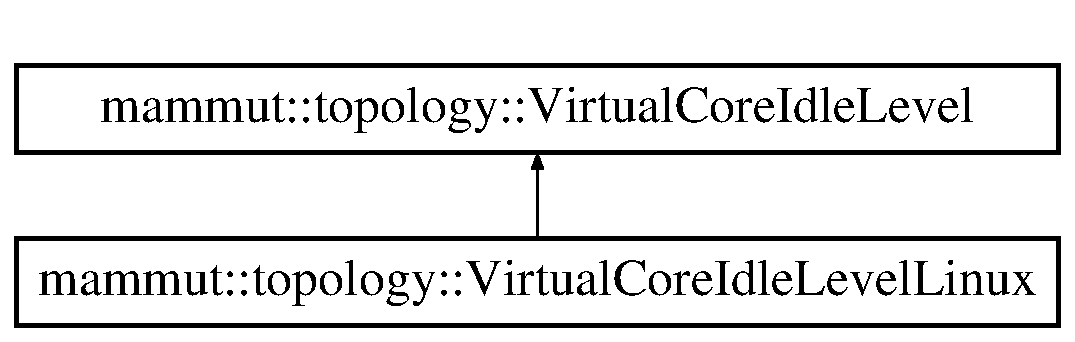
\includegraphics[height=2.000000cm]{classmammut_1_1topology_1_1VirtualCoreIdleLevelLinux}
\end{center}
\end{figure}
\subsection*{Public Member Functions}
\begin{DoxyCompactItemize}
\item 
\hypertarget{classmammut_1_1topology_1_1VirtualCoreIdleLevelLinux_acf7351be50943f449a4e8ea9e5edab8e}{{\bfseries Virtual\-Core\-Idle\-Level\-Linux} (const \hyperlink{classmammut_1_1topology_1_1VirtualCoreLinux}{Virtual\-Core\-Linux} \&virtual\-Core, uint level\-Id)}\label{classmammut_1_1topology_1_1VirtualCoreIdleLevelLinux_acf7351be50943f449a4e8ea9e5edab8e}

\item 
std\-::string \hyperlink{classmammut_1_1topology_1_1VirtualCoreIdleLevelLinux_a4d0c99fe50c44565a89d4e786155cc29}{get\-Name} () const 
\item 
std\-::string \hyperlink{classmammut_1_1topology_1_1VirtualCoreIdleLevelLinux_ada6efb51f70381313b2f3cc1cb3e05fd}{get\-Desc} () const 
\item 
bool \hyperlink{classmammut_1_1topology_1_1VirtualCoreIdleLevelLinux_ac49db1fa35fe5daf4ab06ca83d6de094}{is\-Enableable} () const 
\item 
bool \hyperlink{classmammut_1_1topology_1_1VirtualCoreIdleLevelLinux_ab8a5d122ff265bf697f876b4251f9710}{is\-Enabled} () const 
\item 
void \hyperlink{classmammut_1_1topology_1_1VirtualCoreIdleLevelLinux_a4d82214c9edc3fa8bdc086d11d6d1709}{enable} () const 
\item 
void \hyperlink{classmammut_1_1topology_1_1VirtualCoreIdleLevelLinux_a658a09a3745a68f2891a6296bf8e1535}{disable} () const 
\item 
uint \hyperlink{classmammut_1_1topology_1_1VirtualCoreIdleLevelLinux_a210b830afccb7a6231d8a6298d768bb7}{get\-Exit\-Latency} () const 
\item 
uint \hyperlink{classmammut_1_1topology_1_1VirtualCoreIdleLevelLinux_ac28a040abfa4686d5188cd6f622eb304}{get\-Consumed\-Power} () const 
\item 
uint \hyperlink{classmammut_1_1topology_1_1VirtualCoreIdleLevelLinux_a6c3c8d98625d1827dad0f837fb859e95}{get\-Absolute\-Time} () const 
\item 
uint \hyperlink{classmammut_1_1topology_1_1VirtualCoreIdleLevelLinux_ada0465d3c7030b85356bbd4e9222a44f}{get\-Time} () const 
\item 
void \hyperlink{classmammut_1_1topology_1_1VirtualCoreIdleLevelLinux_a811bcebcc8264a9d033859f5489e7f77}{reset\-Time} ()
\item 
uint \hyperlink{classmammut_1_1topology_1_1VirtualCoreIdleLevelLinux_a0e40c5b94ee5bcef57b09db4b03faeb2}{get\-Absolute\-Count} () const 
\item 
uint \hyperlink{classmammut_1_1topology_1_1VirtualCoreIdleLevelLinux_a877fb980f4d1caf19bac4efc573c89d0}{get\-Count} () const 
\item 
void \hyperlink{classmammut_1_1topology_1_1VirtualCoreIdleLevelLinux_a0e5fed9b3e8a2477c27b9d4e902525bf}{reset\-Count} ()
\end{DoxyCompactItemize}
\subsection*{Additional Inherited Members}


\subsection{Member Function Documentation}
\hypertarget{classmammut_1_1topology_1_1VirtualCoreIdleLevelLinux_a658a09a3745a68f2891a6296bf8e1535}{\index{mammut\-::topology\-::\-Virtual\-Core\-Idle\-Level\-Linux@{mammut\-::topology\-::\-Virtual\-Core\-Idle\-Level\-Linux}!disable@{disable}}
\index{disable@{disable}!mammut::topology::VirtualCoreIdleLevelLinux@{mammut\-::topology\-::\-Virtual\-Core\-Idle\-Level\-Linux}}
\subsubsection[{disable}]{\setlength{\rightskip}{0pt plus 5cm}void mammut\-::topology\-::\-Virtual\-Core\-Idle\-Level\-Linux\-::disable (
\begin{DoxyParamCaption}
{}
\end{DoxyParamCaption}
) const\hspace{0.3cm}{\ttfamily [virtual]}}}\label{classmammut_1_1topology_1_1VirtualCoreIdleLevelLinux_a658a09a3745a68f2891a6296bf8e1535}
Disables this level. 

Implements \hyperlink{classmammut_1_1topology_1_1VirtualCoreIdleLevel_a25ce6958cae064d55055c7940d236f9d}{mammut\-::topology\-::\-Virtual\-Core\-Idle\-Level}.

\hypertarget{classmammut_1_1topology_1_1VirtualCoreIdleLevelLinux_a4d82214c9edc3fa8bdc086d11d6d1709}{\index{mammut\-::topology\-::\-Virtual\-Core\-Idle\-Level\-Linux@{mammut\-::topology\-::\-Virtual\-Core\-Idle\-Level\-Linux}!enable@{enable}}
\index{enable@{enable}!mammut::topology::VirtualCoreIdleLevelLinux@{mammut\-::topology\-::\-Virtual\-Core\-Idle\-Level\-Linux}}
\subsubsection[{enable}]{\setlength{\rightskip}{0pt plus 5cm}void mammut\-::topology\-::\-Virtual\-Core\-Idle\-Level\-Linux\-::enable (
\begin{DoxyParamCaption}
{}
\end{DoxyParamCaption}
) const\hspace{0.3cm}{\ttfamily [virtual]}}}\label{classmammut_1_1topology_1_1VirtualCoreIdleLevelLinux_a4d82214c9edc3fa8bdc086d11d6d1709}
Enables this level. 

Implements \hyperlink{classmammut_1_1topology_1_1VirtualCoreIdleLevel_aac5bccbd57ef3246ac6c268204a337ab}{mammut\-::topology\-::\-Virtual\-Core\-Idle\-Level}.

\hypertarget{classmammut_1_1topology_1_1VirtualCoreIdleLevelLinux_a0e40c5b94ee5bcef57b09db4b03faeb2}{\index{mammut\-::topology\-::\-Virtual\-Core\-Idle\-Level\-Linux@{mammut\-::topology\-::\-Virtual\-Core\-Idle\-Level\-Linux}!get\-Absolute\-Count@{get\-Absolute\-Count}}
\index{get\-Absolute\-Count@{get\-Absolute\-Count}!mammut::topology::VirtualCoreIdleLevelLinux@{mammut\-::topology\-::\-Virtual\-Core\-Idle\-Level\-Linux}}
\subsubsection[{get\-Absolute\-Count}]{\setlength{\rightskip}{0pt plus 5cm}uint mammut\-::topology\-::\-Virtual\-Core\-Idle\-Level\-Linux\-::get\-Absolute\-Count (
\begin{DoxyParamCaption}
{}
\end{DoxyParamCaption}
) const\hspace{0.3cm}{\ttfamily [virtual]}}}\label{classmammut_1_1topology_1_1VirtualCoreIdleLevelLinux_a0e40c5b94ee5bcef57b09db4b03faeb2}
Returns the number of times this level was entered. It is updated only when there is a level change. Accordingly, it could be inaccurate. \begin{DoxyReturn}{Returns}
The number of times this level was entered. 
\end{DoxyReturn}


Implements \hyperlink{classmammut_1_1topology_1_1VirtualCoreIdleLevel_a77b2e87e91dedf6dfa593324875c94fa}{mammut\-::topology\-::\-Virtual\-Core\-Idle\-Level}.

\hypertarget{classmammut_1_1topology_1_1VirtualCoreIdleLevelLinux_a6c3c8d98625d1827dad0f837fb859e95}{\index{mammut\-::topology\-::\-Virtual\-Core\-Idle\-Level\-Linux@{mammut\-::topology\-::\-Virtual\-Core\-Idle\-Level\-Linux}!get\-Absolute\-Time@{get\-Absolute\-Time}}
\index{get\-Absolute\-Time@{get\-Absolute\-Time}!mammut::topology::VirtualCoreIdleLevelLinux@{mammut\-::topology\-::\-Virtual\-Core\-Idle\-Level\-Linux}}
\subsubsection[{get\-Absolute\-Time}]{\setlength{\rightskip}{0pt plus 5cm}uint mammut\-::topology\-::\-Virtual\-Core\-Idle\-Level\-Linux\-::get\-Absolute\-Time (
\begin{DoxyParamCaption}
{}
\end{DoxyParamCaption}
) const\hspace{0.3cm}{\ttfamily [virtual]}}}\label{classmammut_1_1topology_1_1VirtualCoreIdleLevelLinux_a6c3c8d98625d1827dad0f837fb859e95}
Returns the total time spent in this level (in microseconds). It is updated only when there is a level change. Accordingly, it could be inaccurate. \begin{DoxyReturn}{Returns}
The total time spent in this level (in microseconds). 
\end{DoxyReturn}


Implements \hyperlink{classmammut_1_1topology_1_1VirtualCoreIdleLevel_ae841eaa71ad7accb31c37f06f6479030}{mammut\-::topology\-::\-Virtual\-Core\-Idle\-Level}.

\hypertarget{classmammut_1_1topology_1_1VirtualCoreIdleLevelLinux_ac28a040abfa4686d5188cd6f622eb304}{\index{mammut\-::topology\-::\-Virtual\-Core\-Idle\-Level\-Linux@{mammut\-::topology\-::\-Virtual\-Core\-Idle\-Level\-Linux}!get\-Consumed\-Power@{get\-Consumed\-Power}}
\index{get\-Consumed\-Power@{get\-Consumed\-Power}!mammut::topology::VirtualCoreIdleLevelLinux@{mammut\-::topology\-::\-Virtual\-Core\-Idle\-Level\-Linux}}
\subsubsection[{get\-Consumed\-Power}]{\setlength{\rightskip}{0pt plus 5cm}uint mammut\-::topology\-::\-Virtual\-Core\-Idle\-Level\-Linux\-::get\-Consumed\-Power (
\begin{DoxyParamCaption}
{}
\end{DoxyParamCaption}
) const\hspace{0.3cm}{\ttfamily [virtual]}}}\label{classmammut_1_1topology_1_1VirtualCoreIdleLevelLinux_ac28a040abfa4686d5188cd6f622eb304}
Returns the power consumed while in this level (in milliwatts). \begin{DoxyReturn}{Returns}
The power consumed while in this level (in milliwatts). 
\end{DoxyReturn}


Implements \hyperlink{classmammut_1_1topology_1_1VirtualCoreIdleLevel_a0be5f6e317cbfeb8825a21f13ae3e78d}{mammut\-::topology\-::\-Virtual\-Core\-Idle\-Level}.

\hypertarget{classmammut_1_1topology_1_1VirtualCoreIdleLevelLinux_a877fb980f4d1caf19bac4efc573c89d0}{\index{mammut\-::topology\-::\-Virtual\-Core\-Idle\-Level\-Linux@{mammut\-::topology\-::\-Virtual\-Core\-Idle\-Level\-Linux}!get\-Count@{get\-Count}}
\index{get\-Count@{get\-Count}!mammut::topology::VirtualCoreIdleLevelLinux@{mammut\-::topology\-::\-Virtual\-Core\-Idle\-Level\-Linux}}
\subsubsection[{get\-Count}]{\setlength{\rightskip}{0pt plus 5cm}uint mammut\-::topology\-::\-Virtual\-Core\-Idle\-Level\-Linux\-::get\-Count (
\begin{DoxyParamCaption}
{}
\end{DoxyParamCaption}
) const\hspace{0.3cm}{\ttfamily [virtual]}}}\label{classmammut_1_1topology_1_1VirtualCoreIdleLevelLinux_a877fb980f4d1caf19bac4efc573c89d0}
Returns the number of times this level was entered. since the last call of \hyperlink{classmammut_1_1topology_1_1VirtualCoreIdleLevelLinux_a0e5fed9b3e8a2477c27b9d4e902525bf}{reset\-Count()} (or since the creation of this object). It is updated only when there is a level change. Accordingly, it could be inaccurate. \begin{DoxyReturn}{Returns}
The number of times this level was entered. 
\end{DoxyReturn}


Implements \hyperlink{classmammut_1_1topology_1_1VirtualCoreIdleLevel_a031d27afe2c4a164f35fc2c2eeaa22ca}{mammut\-::topology\-::\-Virtual\-Core\-Idle\-Level}.

\hypertarget{classmammut_1_1topology_1_1VirtualCoreIdleLevelLinux_ada6efb51f70381313b2f3cc1cb3e05fd}{\index{mammut\-::topology\-::\-Virtual\-Core\-Idle\-Level\-Linux@{mammut\-::topology\-::\-Virtual\-Core\-Idle\-Level\-Linux}!get\-Desc@{get\-Desc}}
\index{get\-Desc@{get\-Desc}!mammut::topology::VirtualCoreIdleLevelLinux@{mammut\-::topology\-::\-Virtual\-Core\-Idle\-Level\-Linux}}
\subsubsection[{get\-Desc}]{\setlength{\rightskip}{0pt plus 5cm}std\-::string mammut\-::topology\-::\-Virtual\-Core\-Idle\-Level\-Linux\-::get\-Desc (
\begin{DoxyParamCaption}
{}
\end{DoxyParamCaption}
) const\hspace{0.3cm}{\ttfamily [virtual]}}}\label{classmammut_1_1topology_1_1VirtualCoreIdleLevelLinux_ada6efb51f70381313b2f3cc1cb3e05fd}
Returns a small description about this level. \begin{DoxyReturn}{Returns}
A small description about this level. 
\end{DoxyReturn}


Implements \hyperlink{classmammut_1_1topology_1_1VirtualCoreIdleLevel_af2542933dbfe7e83ff9c522a43d96d45}{mammut\-::topology\-::\-Virtual\-Core\-Idle\-Level}.

\hypertarget{classmammut_1_1topology_1_1VirtualCoreIdleLevelLinux_a210b830afccb7a6231d8a6298d768bb7}{\index{mammut\-::topology\-::\-Virtual\-Core\-Idle\-Level\-Linux@{mammut\-::topology\-::\-Virtual\-Core\-Idle\-Level\-Linux}!get\-Exit\-Latency@{get\-Exit\-Latency}}
\index{get\-Exit\-Latency@{get\-Exit\-Latency}!mammut::topology::VirtualCoreIdleLevelLinux@{mammut\-::topology\-::\-Virtual\-Core\-Idle\-Level\-Linux}}
\subsubsection[{get\-Exit\-Latency}]{\setlength{\rightskip}{0pt plus 5cm}uint mammut\-::topology\-::\-Virtual\-Core\-Idle\-Level\-Linux\-::get\-Exit\-Latency (
\begin{DoxyParamCaption}
{}
\end{DoxyParamCaption}
) const\hspace{0.3cm}{\ttfamily [virtual]}}}\label{classmammut_1_1topology_1_1VirtualCoreIdleLevelLinux_a210b830afccb7a6231d8a6298d768bb7}
Returns the latency to exit from this level (in microseconds). \begin{DoxyReturn}{Returns}
The latency to exit from this level (in microseconds). 
\end{DoxyReturn}


Implements \hyperlink{classmammut_1_1topology_1_1VirtualCoreIdleLevel_ab4ab28cce2c5b0d46b94cb0bae02bba5}{mammut\-::topology\-::\-Virtual\-Core\-Idle\-Level}.

\hypertarget{classmammut_1_1topology_1_1VirtualCoreIdleLevelLinux_a4d0c99fe50c44565a89d4e786155cc29}{\index{mammut\-::topology\-::\-Virtual\-Core\-Idle\-Level\-Linux@{mammut\-::topology\-::\-Virtual\-Core\-Idle\-Level\-Linux}!get\-Name@{get\-Name}}
\index{get\-Name@{get\-Name}!mammut::topology::VirtualCoreIdleLevelLinux@{mammut\-::topology\-::\-Virtual\-Core\-Idle\-Level\-Linux}}
\subsubsection[{get\-Name}]{\setlength{\rightskip}{0pt plus 5cm}std\-::string mammut\-::topology\-::\-Virtual\-Core\-Idle\-Level\-Linux\-::get\-Name (
\begin{DoxyParamCaption}
{}
\end{DoxyParamCaption}
) const\hspace{0.3cm}{\ttfamily [virtual]}}}\label{classmammut_1_1topology_1_1VirtualCoreIdleLevelLinux_a4d0c99fe50c44565a89d4e786155cc29}
Returns the name of this level. \begin{DoxyReturn}{Returns}
The name of this level. 
\end{DoxyReturn}


Implements \hyperlink{classmammut_1_1topology_1_1VirtualCoreIdleLevel_a0e11b685cd38c09e4e6fd7610670ffd5}{mammut\-::topology\-::\-Virtual\-Core\-Idle\-Level}.

\hypertarget{classmammut_1_1topology_1_1VirtualCoreIdleLevelLinux_ada0465d3c7030b85356bbd4e9222a44f}{\index{mammut\-::topology\-::\-Virtual\-Core\-Idle\-Level\-Linux@{mammut\-::topology\-::\-Virtual\-Core\-Idle\-Level\-Linux}!get\-Time@{get\-Time}}
\index{get\-Time@{get\-Time}!mammut::topology::VirtualCoreIdleLevelLinux@{mammut\-::topology\-::\-Virtual\-Core\-Idle\-Level\-Linux}}
\subsubsection[{get\-Time}]{\setlength{\rightskip}{0pt plus 5cm}uint mammut\-::topology\-::\-Virtual\-Core\-Idle\-Level\-Linux\-::get\-Time (
\begin{DoxyParamCaption}
{}
\end{DoxyParamCaption}
) const\hspace{0.3cm}{\ttfamily [virtual]}}}\label{classmammut_1_1topology_1_1VirtualCoreIdleLevelLinux_ada0465d3c7030b85356bbd4e9222a44f}
Returns the total time spent in this level (in microseconds) since the last call of \hyperlink{classmammut_1_1topology_1_1VirtualCoreIdleLevelLinux_a811bcebcc8264a9d033859f5489e7f77}{reset\-Time()} (or since the creation of this object). It is updated only when there is a level change. Accordingly, it could be inaccurate. \begin{DoxyReturn}{Returns}
The total time spent in this level (in microseconds). 
\end{DoxyReturn}


Implements \hyperlink{classmammut_1_1topology_1_1VirtualCoreIdleLevel_a44854d4cd60b782ae2738fff8e86ca6e}{mammut\-::topology\-::\-Virtual\-Core\-Idle\-Level}.

\hypertarget{classmammut_1_1topology_1_1VirtualCoreIdleLevelLinux_ac49db1fa35fe5daf4ab06ca83d6de094}{\index{mammut\-::topology\-::\-Virtual\-Core\-Idle\-Level\-Linux@{mammut\-::topology\-::\-Virtual\-Core\-Idle\-Level\-Linux}!is\-Enableable@{is\-Enableable}}
\index{is\-Enableable@{is\-Enableable}!mammut::topology::VirtualCoreIdleLevelLinux@{mammut\-::topology\-::\-Virtual\-Core\-Idle\-Level\-Linux}}
\subsubsection[{is\-Enableable}]{\setlength{\rightskip}{0pt plus 5cm}bool mammut\-::topology\-::\-Virtual\-Core\-Idle\-Level\-Linux\-::is\-Enableable (
\begin{DoxyParamCaption}
{}
\end{DoxyParamCaption}
) const\hspace{0.3cm}{\ttfamily [virtual]}}}\label{classmammut_1_1topology_1_1VirtualCoreIdleLevelLinux_ac49db1fa35fe5daf4ab06ca83d6de094}
Returns true if this level can be dynamically enabled/disabled. \begin{DoxyReturn}{Returns}
True if this level can be dynamically enabled/disabled. 
\end{DoxyReturn}


Implements \hyperlink{classmammut_1_1topology_1_1VirtualCoreIdleLevel_afac261b8838df4df7f694dab365643d2}{mammut\-::topology\-::\-Virtual\-Core\-Idle\-Level}.

\hypertarget{classmammut_1_1topology_1_1VirtualCoreIdleLevelLinux_ab8a5d122ff265bf697f876b4251f9710}{\index{mammut\-::topology\-::\-Virtual\-Core\-Idle\-Level\-Linux@{mammut\-::topology\-::\-Virtual\-Core\-Idle\-Level\-Linux}!is\-Enabled@{is\-Enabled}}
\index{is\-Enabled@{is\-Enabled}!mammut::topology::VirtualCoreIdleLevelLinux@{mammut\-::topology\-::\-Virtual\-Core\-Idle\-Level\-Linux}}
\subsubsection[{is\-Enabled}]{\setlength{\rightskip}{0pt plus 5cm}bool mammut\-::topology\-::\-Virtual\-Core\-Idle\-Level\-Linux\-::is\-Enabled (
\begin{DoxyParamCaption}
{}
\end{DoxyParamCaption}
) const\hspace{0.3cm}{\ttfamily [virtual]}}}\label{classmammut_1_1topology_1_1VirtualCoreIdleLevelLinux_ab8a5d122ff265bf697f876b4251f9710}
Returns true if this level is enabled. \begin{DoxyReturn}{Returns}
True if this level is enabled, false otherwise. 
\end{DoxyReturn}


Implements \hyperlink{classmammut_1_1topology_1_1VirtualCoreIdleLevel_acabc887668492f3e085aae5bb905558a}{mammut\-::topology\-::\-Virtual\-Core\-Idle\-Level}.

\hypertarget{classmammut_1_1topology_1_1VirtualCoreIdleLevelLinux_a0e5fed9b3e8a2477c27b9d4e902525bf}{\index{mammut\-::topology\-::\-Virtual\-Core\-Idle\-Level\-Linux@{mammut\-::topology\-::\-Virtual\-Core\-Idle\-Level\-Linux}!reset\-Count@{reset\-Count}}
\index{reset\-Count@{reset\-Count}!mammut::topology::VirtualCoreIdleLevelLinux@{mammut\-::topology\-::\-Virtual\-Core\-Idle\-Level\-Linux}}
\subsubsection[{reset\-Count}]{\setlength{\rightskip}{0pt plus 5cm}void mammut\-::topology\-::\-Virtual\-Core\-Idle\-Level\-Linux\-::reset\-Count (
\begin{DoxyParamCaption}
{}
\end{DoxyParamCaption}
)\hspace{0.3cm}{\ttfamily [virtual]}}}\label{classmammut_1_1topology_1_1VirtualCoreIdleLevelLinux_a0e5fed9b3e8a2477c27b9d4e902525bf}
Resets the count of this level. 

Implements \hyperlink{classmammut_1_1topology_1_1VirtualCoreIdleLevel_adf46930dfd0fc152490405f586394fd3}{mammut\-::topology\-::\-Virtual\-Core\-Idle\-Level}.

\hypertarget{classmammut_1_1topology_1_1VirtualCoreIdleLevelLinux_a811bcebcc8264a9d033859f5489e7f77}{\index{mammut\-::topology\-::\-Virtual\-Core\-Idle\-Level\-Linux@{mammut\-::topology\-::\-Virtual\-Core\-Idle\-Level\-Linux}!reset\-Time@{reset\-Time}}
\index{reset\-Time@{reset\-Time}!mammut::topology::VirtualCoreIdleLevelLinux@{mammut\-::topology\-::\-Virtual\-Core\-Idle\-Level\-Linux}}
\subsubsection[{reset\-Time}]{\setlength{\rightskip}{0pt plus 5cm}void mammut\-::topology\-::\-Virtual\-Core\-Idle\-Level\-Linux\-::reset\-Time (
\begin{DoxyParamCaption}
{}
\end{DoxyParamCaption}
)\hspace{0.3cm}{\ttfamily [virtual]}}}\label{classmammut_1_1topology_1_1VirtualCoreIdleLevelLinux_a811bcebcc8264a9d033859f5489e7f77}
Resets the time spent in this level. 

Implements \hyperlink{classmammut_1_1topology_1_1VirtualCoreIdleLevel_a22fff5c84d8b377fa1845cafd0df0112}{mammut\-::topology\-::\-Virtual\-Core\-Idle\-Level}.



The documentation for this class was generated from the following files\-:\begin{DoxyCompactItemize}
\item 
/home/daniele/\-Code/\-Mammut/mammut/topology/topology-\/linux.\-hpp\item 
/home/daniele/\-Code/\-Mammut/mammut/topology/topology-\/linux.\-cpp\end{DoxyCompactItemize}

\hypertarget{classmammut_1_1topology_1_1VirtualCoreIdleLevelRemote}{\section{mammut\-:\-:topology\-:\-:Virtual\-Core\-Idle\-Level\-Remote Class Reference}
\label{classmammut_1_1topology_1_1VirtualCoreIdleLevelRemote}\index{mammut\-::topology\-::\-Virtual\-Core\-Idle\-Level\-Remote@{mammut\-::topology\-::\-Virtual\-Core\-Idle\-Level\-Remote}}
}
Inheritance diagram for mammut\-:\-:topology\-:\-:Virtual\-Core\-Idle\-Level\-Remote\-:\begin{figure}[H]
\begin{center}
\leavevmode
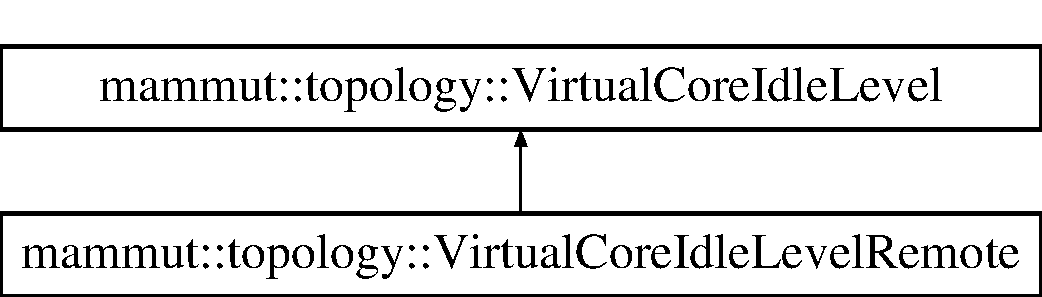
\includegraphics[height=2.000000cm]{classmammut_1_1topology_1_1VirtualCoreIdleLevelRemote}
\end{center}
\end{figure}
\subsection*{Public Member Functions}
\begin{DoxyCompactItemize}
\item 
\hypertarget{classmammut_1_1topology_1_1VirtualCoreIdleLevelRemote_a974bc56791cc3c5960056d1c259eb149}{{\bfseries Virtual\-Core\-Idle\-Level\-Remote} (Virtual\-Core\-Id virtual\-Core\-Id, uint level\-Id, \hyperlink{classmammut_1_1Communicator}{Communicator} $\ast$const communicator)}\label{classmammut_1_1topology_1_1VirtualCoreIdleLevelRemote_a974bc56791cc3c5960056d1c259eb149}

\item 
std\-::string \hyperlink{classmammut_1_1topology_1_1VirtualCoreIdleLevelRemote_a1c940e97ef1bd3a168ce58c468ef6bc9}{get\-Name} () const 
\item 
std\-::string \hyperlink{classmammut_1_1topology_1_1VirtualCoreIdleLevelRemote_a0494e117c0109b94402a18bb97ce97f1}{get\-Desc} () const 
\item 
bool \hyperlink{classmammut_1_1topology_1_1VirtualCoreIdleLevelRemote_a3ba5abd917f53089191ae567fb96bc5a}{is\-Enableable} () const 
\item 
bool \hyperlink{classmammut_1_1topology_1_1VirtualCoreIdleLevelRemote_ad4750a0e885e9ce03d83440a3017c6c0}{is\-Enabled} () const 
\item 
void \hyperlink{classmammut_1_1topology_1_1VirtualCoreIdleLevelRemote_a90fe305ff0f076a6a6c36e6e0a3960f3}{enable} () const 
\item 
void \hyperlink{classmammut_1_1topology_1_1VirtualCoreIdleLevelRemote_aed50c767fc35858e7c1e2bed65566661}{disable} () const 
\item 
uint \hyperlink{classmammut_1_1topology_1_1VirtualCoreIdleLevelRemote_a718403df133e2d0833cbcc7ca2d2b222}{get\-Exit\-Latency} () const 
\item 
uint \hyperlink{classmammut_1_1topology_1_1VirtualCoreIdleLevelRemote_ab7742d64cb5e9db75903df23b5ffac28}{get\-Consumed\-Power} () const 
\item 
uint \hyperlink{classmammut_1_1topology_1_1VirtualCoreIdleLevelRemote_af1837403943f3a4a4e4b9c53051668dd}{get\-Absolute\-Time} () const 
\item 
uint \hyperlink{classmammut_1_1topology_1_1VirtualCoreIdleLevelRemote_a7dd1374dd63b5d5ad59613162d689559}{get\-Time} () const 
\item 
void \hyperlink{classmammut_1_1topology_1_1VirtualCoreIdleLevelRemote_a15c5043370fb096350af0c74d497908e}{reset\-Time} ()
\item 
uint \hyperlink{classmammut_1_1topology_1_1VirtualCoreIdleLevelRemote_a7cb52d93c7fff96c7d8e299b7a0cbdd8}{get\-Absolute\-Count} () const 
\item 
uint \hyperlink{classmammut_1_1topology_1_1VirtualCoreIdleLevelRemote_aa203d9b76cb6b9c721f61c343e342814}{get\-Count} () const 
\item 
void \hyperlink{classmammut_1_1topology_1_1VirtualCoreIdleLevelRemote_aa3f49ed20ca10011d01174fdf6bde3e2}{reset\-Count} ()
\end{DoxyCompactItemize}
\subsection*{Additional Inherited Members}


\subsection{Member Function Documentation}
\hypertarget{classmammut_1_1topology_1_1VirtualCoreIdleLevelRemote_aed50c767fc35858e7c1e2bed65566661}{\index{mammut\-::topology\-::\-Virtual\-Core\-Idle\-Level\-Remote@{mammut\-::topology\-::\-Virtual\-Core\-Idle\-Level\-Remote}!disable@{disable}}
\index{disable@{disable}!mammut::topology::VirtualCoreIdleLevelRemote@{mammut\-::topology\-::\-Virtual\-Core\-Idle\-Level\-Remote}}
\subsubsection[{disable}]{\setlength{\rightskip}{0pt plus 5cm}void mammut\-::topology\-::\-Virtual\-Core\-Idle\-Level\-Remote\-::disable (
\begin{DoxyParamCaption}
{}
\end{DoxyParamCaption}
) const\hspace{0.3cm}{\ttfamily [virtual]}}}\label{classmammut_1_1topology_1_1VirtualCoreIdleLevelRemote_aed50c767fc35858e7c1e2bed65566661}
Disables this level. 

Implements \hyperlink{classmammut_1_1topology_1_1VirtualCoreIdleLevel_a25ce6958cae064d55055c7940d236f9d}{mammut\-::topology\-::\-Virtual\-Core\-Idle\-Level}.

\hypertarget{classmammut_1_1topology_1_1VirtualCoreIdleLevelRemote_a90fe305ff0f076a6a6c36e6e0a3960f3}{\index{mammut\-::topology\-::\-Virtual\-Core\-Idle\-Level\-Remote@{mammut\-::topology\-::\-Virtual\-Core\-Idle\-Level\-Remote}!enable@{enable}}
\index{enable@{enable}!mammut::topology::VirtualCoreIdleLevelRemote@{mammut\-::topology\-::\-Virtual\-Core\-Idle\-Level\-Remote}}
\subsubsection[{enable}]{\setlength{\rightskip}{0pt plus 5cm}void mammut\-::topology\-::\-Virtual\-Core\-Idle\-Level\-Remote\-::enable (
\begin{DoxyParamCaption}
{}
\end{DoxyParamCaption}
) const\hspace{0.3cm}{\ttfamily [virtual]}}}\label{classmammut_1_1topology_1_1VirtualCoreIdleLevelRemote_a90fe305ff0f076a6a6c36e6e0a3960f3}
Enables this level. 

Implements \hyperlink{classmammut_1_1topology_1_1VirtualCoreIdleLevel_aac5bccbd57ef3246ac6c268204a337ab}{mammut\-::topology\-::\-Virtual\-Core\-Idle\-Level}.

\hypertarget{classmammut_1_1topology_1_1VirtualCoreIdleLevelRemote_a7cb52d93c7fff96c7d8e299b7a0cbdd8}{\index{mammut\-::topology\-::\-Virtual\-Core\-Idle\-Level\-Remote@{mammut\-::topology\-::\-Virtual\-Core\-Idle\-Level\-Remote}!get\-Absolute\-Count@{get\-Absolute\-Count}}
\index{get\-Absolute\-Count@{get\-Absolute\-Count}!mammut::topology::VirtualCoreIdleLevelRemote@{mammut\-::topology\-::\-Virtual\-Core\-Idle\-Level\-Remote}}
\subsubsection[{get\-Absolute\-Count}]{\setlength{\rightskip}{0pt plus 5cm}uint mammut\-::topology\-::\-Virtual\-Core\-Idle\-Level\-Remote\-::get\-Absolute\-Count (
\begin{DoxyParamCaption}
{}
\end{DoxyParamCaption}
) const\hspace{0.3cm}{\ttfamily [virtual]}}}\label{classmammut_1_1topology_1_1VirtualCoreIdleLevelRemote_a7cb52d93c7fff96c7d8e299b7a0cbdd8}
Returns the number of times this level was entered. It is updated only when there is a level change. Accordingly, it could be inaccurate. \begin{DoxyReturn}{Returns}
The number of times this level was entered. 
\end{DoxyReturn}


Implements \hyperlink{classmammut_1_1topology_1_1VirtualCoreIdleLevel_a77b2e87e91dedf6dfa593324875c94fa}{mammut\-::topology\-::\-Virtual\-Core\-Idle\-Level}.

\hypertarget{classmammut_1_1topology_1_1VirtualCoreIdleLevelRemote_af1837403943f3a4a4e4b9c53051668dd}{\index{mammut\-::topology\-::\-Virtual\-Core\-Idle\-Level\-Remote@{mammut\-::topology\-::\-Virtual\-Core\-Idle\-Level\-Remote}!get\-Absolute\-Time@{get\-Absolute\-Time}}
\index{get\-Absolute\-Time@{get\-Absolute\-Time}!mammut::topology::VirtualCoreIdleLevelRemote@{mammut\-::topology\-::\-Virtual\-Core\-Idle\-Level\-Remote}}
\subsubsection[{get\-Absolute\-Time}]{\setlength{\rightskip}{0pt plus 5cm}uint mammut\-::topology\-::\-Virtual\-Core\-Idle\-Level\-Remote\-::get\-Absolute\-Time (
\begin{DoxyParamCaption}
{}
\end{DoxyParamCaption}
) const\hspace{0.3cm}{\ttfamily [virtual]}}}\label{classmammut_1_1topology_1_1VirtualCoreIdleLevelRemote_af1837403943f3a4a4e4b9c53051668dd}
Returns the total time spent in this level (in microseconds). It is updated only when there is a level change. Accordingly, it could be inaccurate. \begin{DoxyReturn}{Returns}
The total time spent in this level (in microseconds). 
\end{DoxyReturn}


Implements \hyperlink{classmammut_1_1topology_1_1VirtualCoreIdleLevel_ae841eaa71ad7accb31c37f06f6479030}{mammut\-::topology\-::\-Virtual\-Core\-Idle\-Level}.

\hypertarget{classmammut_1_1topology_1_1VirtualCoreIdleLevelRemote_ab7742d64cb5e9db75903df23b5ffac28}{\index{mammut\-::topology\-::\-Virtual\-Core\-Idle\-Level\-Remote@{mammut\-::topology\-::\-Virtual\-Core\-Idle\-Level\-Remote}!get\-Consumed\-Power@{get\-Consumed\-Power}}
\index{get\-Consumed\-Power@{get\-Consumed\-Power}!mammut::topology::VirtualCoreIdleLevelRemote@{mammut\-::topology\-::\-Virtual\-Core\-Idle\-Level\-Remote}}
\subsubsection[{get\-Consumed\-Power}]{\setlength{\rightskip}{0pt plus 5cm}uint mammut\-::topology\-::\-Virtual\-Core\-Idle\-Level\-Remote\-::get\-Consumed\-Power (
\begin{DoxyParamCaption}
{}
\end{DoxyParamCaption}
) const\hspace{0.3cm}{\ttfamily [virtual]}}}\label{classmammut_1_1topology_1_1VirtualCoreIdleLevelRemote_ab7742d64cb5e9db75903df23b5ffac28}
Returns the power consumed while in this level (in milliwatts). \begin{DoxyReturn}{Returns}
The power consumed while in this level (in milliwatts). 
\end{DoxyReturn}


Implements \hyperlink{classmammut_1_1topology_1_1VirtualCoreIdleLevel_a0be5f6e317cbfeb8825a21f13ae3e78d}{mammut\-::topology\-::\-Virtual\-Core\-Idle\-Level}.

\hypertarget{classmammut_1_1topology_1_1VirtualCoreIdleLevelRemote_aa203d9b76cb6b9c721f61c343e342814}{\index{mammut\-::topology\-::\-Virtual\-Core\-Idle\-Level\-Remote@{mammut\-::topology\-::\-Virtual\-Core\-Idle\-Level\-Remote}!get\-Count@{get\-Count}}
\index{get\-Count@{get\-Count}!mammut::topology::VirtualCoreIdleLevelRemote@{mammut\-::topology\-::\-Virtual\-Core\-Idle\-Level\-Remote}}
\subsubsection[{get\-Count}]{\setlength{\rightskip}{0pt plus 5cm}uint mammut\-::topology\-::\-Virtual\-Core\-Idle\-Level\-Remote\-::get\-Count (
\begin{DoxyParamCaption}
{}
\end{DoxyParamCaption}
) const\hspace{0.3cm}{\ttfamily [virtual]}}}\label{classmammut_1_1topology_1_1VirtualCoreIdleLevelRemote_aa203d9b76cb6b9c721f61c343e342814}
Returns the number of times this level was entered. since the last call of \hyperlink{classmammut_1_1topology_1_1VirtualCoreIdleLevelRemote_aa3f49ed20ca10011d01174fdf6bde3e2}{reset\-Count()} (or since the creation of this object). It is updated only when there is a level change. Accordingly, it could be inaccurate. \begin{DoxyReturn}{Returns}
The number of times this level was entered. 
\end{DoxyReturn}


Implements \hyperlink{classmammut_1_1topology_1_1VirtualCoreIdleLevel_a031d27afe2c4a164f35fc2c2eeaa22ca}{mammut\-::topology\-::\-Virtual\-Core\-Idle\-Level}.

\hypertarget{classmammut_1_1topology_1_1VirtualCoreIdleLevelRemote_a0494e117c0109b94402a18bb97ce97f1}{\index{mammut\-::topology\-::\-Virtual\-Core\-Idle\-Level\-Remote@{mammut\-::topology\-::\-Virtual\-Core\-Idle\-Level\-Remote}!get\-Desc@{get\-Desc}}
\index{get\-Desc@{get\-Desc}!mammut::topology::VirtualCoreIdleLevelRemote@{mammut\-::topology\-::\-Virtual\-Core\-Idle\-Level\-Remote}}
\subsubsection[{get\-Desc}]{\setlength{\rightskip}{0pt plus 5cm}std\-::string mammut\-::topology\-::\-Virtual\-Core\-Idle\-Level\-Remote\-::get\-Desc (
\begin{DoxyParamCaption}
{}
\end{DoxyParamCaption}
) const\hspace{0.3cm}{\ttfamily [virtual]}}}\label{classmammut_1_1topology_1_1VirtualCoreIdleLevelRemote_a0494e117c0109b94402a18bb97ce97f1}
Returns a small description about this level. \begin{DoxyReturn}{Returns}
A small description about this level. 
\end{DoxyReturn}


Implements \hyperlink{classmammut_1_1topology_1_1VirtualCoreIdleLevel_af2542933dbfe7e83ff9c522a43d96d45}{mammut\-::topology\-::\-Virtual\-Core\-Idle\-Level}.

\hypertarget{classmammut_1_1topology_1_1VirtualCoreIdleLevelRemote_a718403df133e2d0833cbcc7ca2d2b222}{\index{mammut\-::topology\-::\-Virtual\-Core\-Idle\-Level\-Remote@{mammut\-::topology\-::\-Virtual\-Core\-Idle\-Level\-Remote}!get\-Exit\-Latency@{get\-Exit\-Latency}}
\index{get\-Exit\-Latency@{get\-Exit\-Latency}!mammut::topology::VirtualCoreIdleLevelRemote@{mammut\-::topology\-::\-Virtual\-Core\-Idle\-Level\-Remote}}
\subsubsection[{get\-Exit\-Latency}]{\setlength{\rightskip}{0pt plus 5cm}uint mammut\-::topology\-::\-Virtual\-Core\-Idle\-Level\-Remote\-::get\-Exit\-Latency (
\begin{DoxyParamCaption}
{}
\end{DoxyParamCaption}
) const\hspace{0.3cm}{\ttfamily [virtual]}}}\label{classmammut_1_1topology_1_1VirtualCoreIdleLevelRemote_a718403df133e2d0833cbcc7ca2d2b222}
Returns the latency to exit from this level (in microseconds). \begin{DoxyReturn}{Returns}
The latency to exit from this level (in microseconds). 
\end{DoxyReturn}


Implements \hyperlink{classmammut_1_1topology_1_1VirtualCoreIdleLevel_ab4ab28cce2c5b0d46b94cb0bae02bba5}{mammut\-::topology\-::\-Virtual\-Core\-Idle\-Level}.

\hypertarget{classmammut_1_1topology_1_1VirtualCoreIdleLevelRemote_a1c940e97ef1bd3a168ce58c468ef6bc9}{\index{mammut\-::topology\-::\-Virtual\-Core\-Idle\-Level\-Remote@{mammut\-::topology\-::\-Virtual\-Core\-Idle\-Level\-Remote}!get\-Name@{get\-Name}}
\index{get\-Name@{get\-Name}!mammut::topology::VirtualCoreIdleLevelRemote@{mammut\-::topology\-::\-Virtual\-Core\-Idle\-Level\-Remote}}
\subsubsection[{get\-Name}]{\setlength{\rightskip}{0pt plus 5cm}std\-::string mammut\-::topology\-::\-Virtual\-Core\-Idle\-Level\-Remote\-::get\-Name (
\begin{DoxyParamCaption}
{}
\end{DoxyParamCaption}
) const\hspace{0.3cm}{\ttfamily [virtual]}}}\label{classmammut_1_1topology_1_1VirtualCoreIdleLevelRemote_a1c940e97ef1bd3a168ce58c468ef6bc9}
Returns the name of this level. \begin{DoxyReturn}{Returns}
The name of this level. 
\end{DoxyReturn}


Implements \hyperlink{classmammut_1_1topology_1_1VirtualCoreIdleLevel_a0e11b685cd38c09e4e6fd7610670ffd5}{mammut\-::topology\-::\-Virtual\-Core\-Idle\-Level}.

\hypertarget{classmammut_1_1topology_1_1VirtualCoreIdleLevelRemote_a7dd1374dd63b5d5ad59613162d689559}{\index{mammut\-::topology\-::\-Virtual\-Core\-Idle\-Level\-Remote@{mammut\-::topology\-::\-Virtual\-Core\-Idle\-Level\-Remote}!get\-Time@{get\-Time}}
\index{get\-Time@{get\-Time}!mammut::topology::VirtualCoreIdleLevelRemote@{mammut\-::topology\-::\-Virtual\-Core\-Idle\-Level\-Remote}}
\subsubsection[{get\-Time}]{\setlength{\rightskip}{0pt plus 5cm}uint mammut\-::topology\-::\-Virtual\-Core\-Idle\-Level\-Remote\-::get\-Time (
\begin{DoxyParamCaption}
{}
\end{DoxyParamCaption}
) const\hspace{0.3cm}{\ttfamily [virtual]}}}\label{classmammut_1_1topology_1_1VirtualCoreIdleLevelRemote_a7dd1374dd63b5d5ad59613162d689559}
Returns the total time spent in this level (in microseconds) since the last call of \hyperlink{classmammut_1_1topology_1_1VirtualCoreIdleLevelRemote_a15c5043370fb096350af0c74d497908e}{reset\-Time()} (or since the creation of this object). It is updated only when there is a level change. Accordingly, it could be inaccurate. \begin{DoxyReturn}{Returns}
The total time spent in this level (in microseconds). 
\end{DoxyReturn}


Implements \hyperlink{classmammut_1_1topology_1_1VirtualCoreIdleLevel_a44854d4cd60b782ae2738fff8e86ca6e}{mammut\-::topology\-::\-Virtual\-Core\-Idle\-Level}.

\hypertarget{classmammut_1_1topology_1_1VirtualCoreIdleLevelRemote_a3ba5abd917f53089191ae567fb96bc5a}{\index{mammut\-::topology\-::\-Virtual\-Core\-Idle\-Level\-Remote@{mammut\-::topology\-::\-Virtual\-Core\-Idle\-Level\-Remote}!is\-Enableable@{is\-Enableable}}
\index{is\-Enableable@{is\-Enableable}!mammut::topology::VirtualCoreIdleLevelRemote@{mammut\-::topology\-::\-Virtual\-Core\-Idle\-Level\-Remote}}
\subsubsection[{is\-Enableable}]{\setlength{\rightskip}{0pt plus 5cm}bool mammut\-::topology\-::\-Virtual\-Core\-Idle\-Level\-Remote\-::is\-Enableable (
\begin{DoxyParamCaption}
{}
\end{DoxyParamCaption}
) const\hspace{0.3cm}{\ttfamily [virtual]}}}\label{classmammut_1_1topology_1_1VirtualCoreIdleLevelRemote_a3ba5abd917f53089191ae567fb96bc5a}
Returns true if this level can be dynamically enabled/disabled. \begin{DoxyReturn}{Returns}
True if this level can be dynamically enabled/disabled. 
\end{DoxyReturn}


Implements \hyperlink{classmammut_1_1topology_1_1VirtualCoreIdleLevel_afac261b8838df4df7f694dab365643d2}{mammut\-::topology\-::\-Virtual\-Core\-Idle\-Level}.

\hypertarget{classmammut_1_1topology_1_1VirtualCoreIdleLevelRemote_ad4750a0e885e9ce03d83440a3017c6c0}{\index{mammut\-::topology\-::\-Virtual\-Core\-Idle\-Level\-Remote@{mammut\-::topology\-::\-Virtual\-Core\-Idle\-Level\-Remote}!is\-Enabled@{is\-Enabled}}
\index{is\-Enabled@{is\-Enabled}!mammut::topology::VirtualCoreIdleLevelRemote@{mammut\-::topology\-::\-Virtual\-Core\-Idle\-Level\-Remote}}
\subsubsection[{is\-Enabled}]{\setlength{\rightskip}{0pt plus 5cm}bool mammut\-::topology\-::\-Virtual\-Core\-Idle\-Level\-Remote\-::is\-Enabled (
\begin{DoxyParamCaption}
{}
\end{DoxyParamCaption}
) const\hspace{0.3cm}{\ttfamily [virtual]}}}\label{classmammut_1_1topology_1_1VirtualCoreIdleLevelRemote_ad4750a0e885e9ce03d83440a3017c6c0}
Returns true if this level is enabled. \begin{DoxyReturn}{Returns}
True if this level is enabled, false otherwise. 
\end{DoxyReturn}


Implements \hyperlink{classmammut_1_1topology_1_1VirtualCoreIdleLevel_acabc887668492f3e085aae5bb905558a}{mammut\-::topology\-::\-Virtual\-Core\-Idle\-Level}.

\hypertarget{classmammut_1_1topology_1_1VirtualCoreIdleLevelRemote_aa3f49ed20ca10011d01174fdf6bde3e2}{\index{mammut\-::topology\-::\-Virtual\-Core\-Idle\-Level\-Remote@{mammut\-::topology\-::\-Virtual\-Core\-Idle\-Level\-Remote}!reset\-Count@{reset\-Count}}
\index{reset\-Count@{reset\-Count}!mammut::topology::VirtualCoreIdleLevelRemote@{mammut\-::topology\-::\-Virtual\-Core\-Idle\-Level\-Remote}}
\subsubsection[{reset\-Count}]{\setlength{\rightskip}{0pt plus 5cm}void mammut\-::topology\-::\-Virtual\-Core\-Idle\-Level\-Remote\-::reset\-Count (
\begin{DoxyParamCaption}
{}
\end{DoxyParamCaption}
)\hspace{0.3cm}{\ttfamily [virtual]}}}\label{classmammut_1_1topology_1_1VirtualCoreIdleLevelRemote_aa3f49ed20ca10011d01174fdf6bde3e2}
Resets the count of this level. 

Implements \hyperlink{classmammut_1_1topology_1_1VirtualCoreIdleLevel_adf46930dfd0fc152490405f586394fd3}{mammut\-::topology\-::\-Virtual\-Core\-Idle\-Level}.

\hypertarget{classmammut_1_1topology_1_1VirtualCoreIdleLevelRemote_a15c5043370fb096350af0c74d497908e}{\index{mammut\-::topology\-::\-Virtual\-Core\-Idle\-Level\-Remote@{mammut\-::topology\-::\-Virtual\-Core\-Idle\-Level\-Remote}!reset\-Time@{reset\-Time}}
\index{reset\-Time@{reset\-Time}!mammut::topology::VirtualCoreIdleLevelRemote@{mammut\-::topology\-::\-Virtual\-Core\-Idle\-Level\-Remote}}
\subsubsection[{reset\-Time}]{\setlength{\rightskip}{0pt plus 5cm}void mammut\-::topology\-::\-Virtual\-Core\-Idle\-Level\-Remote\-::reset\-Time (
\begin{DoxyParamCaption}
{}
\end{DoxyParamCaption}
)\hspace{0.3cm}{\ttfamily [virtual]}}}\label{classmammut_1_1topology_1_1VirtualCoreIdleLevelRemote_a15c5043370fb096350af0c74d497908e}
Resets the time spent in this level. 

Implements \hyperlink{classmammut_1_1topology_1_1VirtualCoreIdleLevel_a22fff5c84d8b377fa1845cafd0df0112}{mammut\-::topology\-::\-Virtual\-Core\-Idle\-Level}.



The documentation for this class was generated from the following file\-:\begin{DoxyCompactItemize}
\item 
/home/daniele/\-Code/\-Mammut/mammut/topology/topology-\/remote.\-hpp\end{DoxyCompactItemize}

\hypertarget{classmammut_1_1topology_1_1VirtualCoreLinux}{\section{mammut\-:\-:topology\-:\-:Virtual\-Core\-Linux Class Reference}
\label{classmammut_1_1topology_1_1VirtualCoreLinux}\index{mammut\-::topology\-::\-Virtual\-Core\-Linux@{mammut\-::topology\-::\-Virtual\-Core\-Linux}}
}
Inheritance diagram for mammut\-:\-:topology\-:\-:Virtual\-Core\-Linux\-:\begin{figure}[H]
\begin{center}
\leavevmode
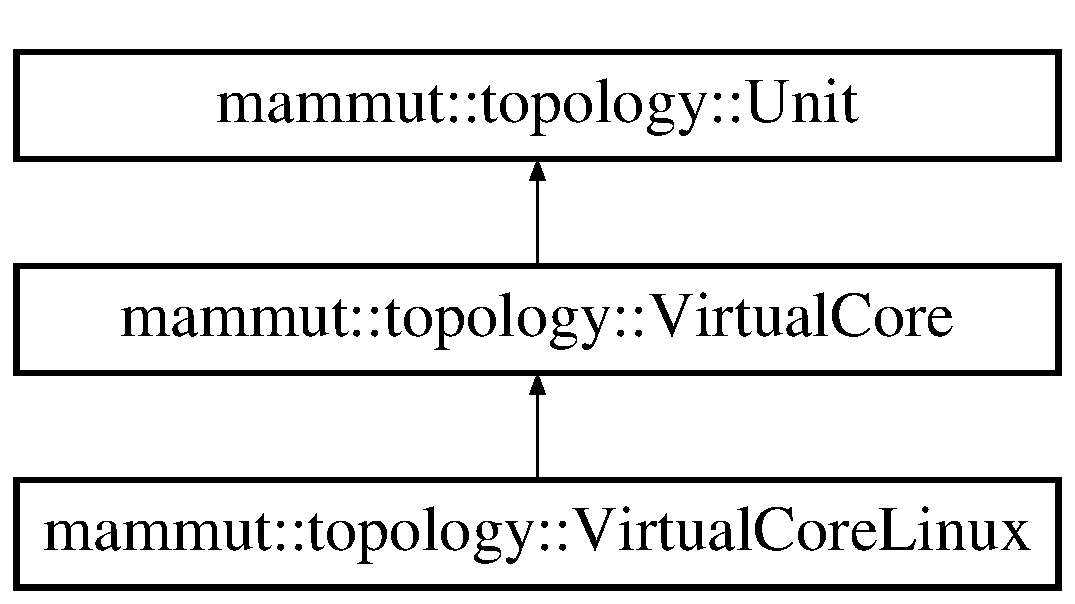
\includegraphics[height=3.000000cm]{classmammut_1_1topology_1_1VirtualCoreLinux}
\end{center}
\end{figure}
\subsection*{Public Member Functions}
\begin{DoxyCompactItemize}
\item 
\hypertarget{classmammut_1_1topology_1_1VirtualCoreLinux_a322e1ea00f2b3bb8a7b42483811d2d2e}{{\bfseries Virtual\-Core\-Linux} (Cpu\-Id cpu\-Id, Physical\-Core\-Id physical\-Core\-Id, Virtual\-Core\-Id virtual\-Core\-Id)}\label{classmammut_1_1topology_1_1VirtualCoreLinux_a322e1ea00f2b3bb8a7b42483811d2d2e}

\item 
bool \hyperlink{classmammut_1_1topology_1_1VirtualCoreLinux_ac05cd4f3131857160bb438b0abfacfd6}{has\-Flag} (const std\-::string \&flag\-Name) const 
\item 
uint64\-\_\-t \hyperlink{classmammut_1_1topology_1_1VirtualCoreLinux_acf8e7e73687907450f243d5c8014a6cb}{get\-Absolute\-Ticks} () const 
\item 
void \hyperlink{classmammut_1_1topology_1_1VirtualCoreLinux_a9e06cca87b5879be4fe433bd409098e4}{maximize\-Utilization} () const 
\item 
void \hyperlink{classmammut_1_1topology_1_1VirtualCoreLinux_a9091e0404bacb86772ee34c3c24e5713}{reset\-Utilization} () const 
\item 
double \hyperlink{classmammut_1_1topology_1_1VirtualCoreLinux_a8e637a85c90167e45f6a051ac1b689d9}{get\-Idle\-Time} () const 
\item 
void \hyperlink{classmammut_1_1topology_1_1VirtualCoreLinux_aaa38f4ffc17855b1cd97c4c7b2002eb6}{reset\-Idle\-Time} ()
\item 
bool \hyperlink{classmammut_1_1topology_1_1VirtualCoreLinux_a055bb4d39491bc01f36e2c3eb9f76ca8}{is\-Hot\-Pluggable} () const 
\item 
bool \hyperlink{classmammut_1_1topology_1_1VirtualCoreLinux_a9967ee4dc065b3478b7456439432c853}{is\-Hot\-Plugged} () const 
\item 
void \hyperlink{classmammut_1_1topology_1_1VirtualCoreLinux_acbe52ae75f315f953d7945719a044d80}{hot\-Plug} () const 
\item 
void \hyperlink{classmammut_1_1topology_1_1VirtualCoreLinux_a8021dd7fbaeb546770d3752ede651e78}{hot\-Unplug} () const 
\item 
std\-::vector\\*
$<$ \hyperlink{classmammut_1_1topology_1_1VirtualCoreIdleLevel}{Virtual\-Core\-Idle\-Level} $\ast$ $>$ \hyperlink{classmammut_1_1topology_1_1VirtualCoreLinux_a615953356164817ea8d416f439ac0f72}{get\-Idle\-Levels} () const 
\end{DoxyCompactItemize}
\subsection*{Additional Inherited Members}


\subsection{Member Function Documentation}
\hypertarget{classmammut_1_1topology_1_1VirtualCoreLinux_acf8e7e73687907450f243d5c8014a6cb}{\index{mammut\-::topology\-::\-Virtual\-Core\-Linux@{mammut\-::topology\-::\-Virtual\-Core\-Linux}!get\-Absolute\-Ticks@{get\-Absolute\-Ticks}}
\index{get\-Absolute\-Ticks@{get\-Absolute\-Ticks}!mammut::topology::VirtualCoreLinux@{mammut\-::topology\-::\-Virtual\-Core\-Linux}}
\subsubsection[{get\-Absolute\-Ticks}]{\setlength{\rightskip}{0pt plus 5cm}uint64\-\_\-t mammut\-::topology\-::\-Virtual\-Core\-Linux\-::get\-Absolute\-Ticks (
\begin{DoxyParamCaption}
{}
\end{DoxyParamCaption}
) const\hspace{0.3cm}{\ttfamily [virtual]}}}\label{classmammut_1_1topology_1_1VirtualCoreLinux_acf8e7e73687907450f243d5c8014a6cb}
Gets the clock ticks of this virtual core. \begin{DoxyReturn}{Returns}
The clock ticks of this virtual core. If 0 is returned, ticks are not available. A\-T\-T\-E\-N\-T\-I\-O\-N\-: In general, ticks may change with frequency, i.\-e. the amount of ticks per second at 1\-G\-Hz may be different from the amount of ticks per second at 2\-G\-Hz. To check if ticks do not change with the frequency, you should use '\hyperlink{classmammut_1_1topology_1_1VirtualCore_a82bf6ba883ee5bdc4ef4b3c0fb300207}{are\-Ticks\-Constant()}' call. 
\end{DoxyReturn}


Implements \hyperlink{classmammut_1_1topology_1_1VirtualCore_a0b1ac9c138d1ed5e8eceb38e619e1e65}{mammut\-::topology\-::\-Virtual\-Core}.

\hypertarget{classmammut_1_1topology_1_1VirtualCoreLinux_a615953356164817ea8d416f439ac0f72}{\index{mammut\-::topology\-::\-Virtual\-Core\-Linux@{mammut\-::topology\-::\-Virtual\-Core\-Linux}!get\-Idle\-Levels@{get\-Idle\-Levels}}
\index{get\-Idle\-Levels@{get\-Idle\-Levels}!mammut::topology::VirtualCoreLinux@{mammut\-::topology\-::\-Virtual\-Core\-Linux}}
\subsubsection[{get\-Idle\-Levels}]{\setlength{\rightskip}{0pt plus 5cm}std\-::vector$<$ {\bf Virtual\-Core\-Idle\-Level} $\ast$ $>$ mammut\-::topology\-::\-Virtual\-Core\-Linux\-::get\-Idle\-Levels (
\begin{DoxyParamCaption}
{}
\end{DoxyParamCaption}
) const\hspace{0.3cm}{\ttfamily [virtual]}}}\label{classmammut_1_1topology_1_1VirtualCoreLinux_a615953356164817ea8d416f439ac0f72}
Returns the idle levels (C-\/\-States) supported by this virtual core. \begin{DoxyReturn}{Returns}
The idle levels supported by this virtual core. If the vector is empty, no idle levels are supported. 
\end{DoxyReturn}


Implements \hyperlink{classmammut_1_1topology_1_1VirtualCore_a841dd64b1b74b28a0533cc1aa9d8cb84}{mammut\-::topology\-::\-Virtual\-Core}.

\hypertarget{classmammut_1_1topology_1_1VirtualCoreLinux_a8e637a85c90167e45f6a051ac1b689d9}{\index{mammut\-::topology\-::\-Virtual\-Core\-Linux@{mammut\-::topology\-::\-Virtual\-Core\-Linux}!get\-Idle\-Time@{get\-Idle\-Time}}
\index{get\-Idle\-Time@{get\-Idle\-Time}!mammut::topology::VirtualCoreLinux@{mammut\-::topology\-::\-Virtual\-Core\-Linux}}
\subsubsection[{get\-Idle\-Time}]{\setlength{\rightskip}{0pt plus 5cm}double mammut\-::topology\-::\-Virtual\-Core\-Linux\-::get\-Idle\-Time (
\begin{DoxyParamCaption}
{}
\end{DoxyParamCaption}
) const\hspace{0.3cm}{\ttfamily [virtual]}}}\label{classmammut_1_1topology_1_1VirtualCoreLinux_a8e637a85c90167e45f6a051ac1b689d9}
Returns the number of microseconds that this virtual core have been idle since the last call of \hyperlink{classmammut_1_1topology_1_1VirtualCoreLinux_aaa38f4ffc17855b1cd97c4c7b2002eb6}{reset\-Idle\-Time()} (or since the creation of this virtual core handler). \begin{DoxyReturn}{Returns}
The number of microseconds that this virtual core have been idle. 
\end{DoxyReturn}


Implements \hyperlink{classmammut_1_1topology_1_1VirtualCore_ad4a33cf2323e7b05537485e4b08a4f12}{mammut\-::topology\-::\-Virtual\-Core}.

\hypertarget{classmammut_1_1topology_1_1VirtualCoreLinux_ac05cd4f3131857160bb438b0abfacfd6}{\index{mammut\-::topology\-::\-Virtual\-Core\-Linux@{mammut\-::topology\-::\-Virtual\-Core\-Linux}!has\-Flag@{has\-Flag}}
\index{has\-Flag@{has\-Flag}!mammut::topology::VirtualCoreLinux@{mammut\-::topology\-::\-Virtual\-Core\-Linux}}
\subsubsection[{has\-Flag}]{\setlength{\rightskip}{0pt plus 5cm}bool mammut\-::topology\-::\-Virtual\-Core\-Linux\-::has\-Flag (
\begin{DoxyParamCaption}
\item[{const std\-::string \&}]{flag\-Name}
\end{DoxyParamCaption}
) const\hspace{0.3cm}{\ttfamily [virtual]}}}\label{classmammut_1_1topology_1_1VirtualCoreLinux_ac05cd4f3131857160bb438b0abfacfd6}
Checks if this virtual core has a specific flag Find the section of this virtual core.

We finished the section of this virtual core. 

Implements \hyperlink{classmammut_1_1topology_1_1VirtualCore_aa9f4400708c97197f66bcd11aa0eb990}{mammut\-::topology\-::\-Virtual\-Core}.

\hypertarget{classmammut_1_1topology_1_1VirtualCoreLinux_acbe52ae75f315f953d7945719a044d80}{\index{mammut\-::topology\-::\-Virtual\-Core\-Linux@{mammut\-::topology\-::\-Virtual\-Core\-Linux}!hot\-Plug@{hot\-Plug}}
\index{hot\-Plug@{hot\-Plug}!mammut::topology::VirtualCoreLinux@{mammut\-::topology\-::\-Virtual\-Core\-Linux}}
\subsubsection[{hot\-Plug}]{\setlength{\rightskip}{0pt plus 5cm}void mammut\-::topology\-::\-Virtual\-Core\-Linux\-::hot\-Plug (
\begin{DoxyParamCaption}
{}
\end{DoxyParamCaption}
) const\hspace{0.3cm}{\ttfamily [virtual]}}}\label{classmammut_1_1topology_1_1VirtualCoreLinux_acbe52ae75f315f953d7945719a044d80}
Hotplugs this virtual core. If this core is not hot-\/pluggable, nothing is done. 

Implements \hyperlink{classmammut_1_1topology_1_1VirtualCore_a7674d352e60bb8d9c183ca54f62b383d}{mammut\-::topology\-::\-Virtual\-Core}.

\hypertarget{classmammut_1_1topology_1_1VirtualCoreLinux_a8021dd7fbaeb546770d3752ede651e78}{\index{mammut\-::topology\-::\-Virtual\-Core\-Linux@{mammut\-::topology\-::\-Virtual\-Core\-Linux}!hot\-Unplug@{hot\-Unplug}}
\index{hot\-Unplug@{hot\-Unplug}!mammut::topology::VirtualCoreLinux@{mammut\-::topology\-::\-Virtual\-Core\-Linux}}
\subsubsection[{hot\-Unplug}]{\setlength{\rightskip}{0pt plus 5cm}void mammut\-::topology\-::\-Virtual\-Core\-Linux\-::hot\-Unplug (
\begin{DoxyParamCaption}
{}
\end{DoxyParamCaption}
) const\hspace{0.3cm}{\ttfamily [virtual]}}}\label{classmammut_1_1topology_1_1VirtualCoreLinux_a8021dd7fbaeb546770d3752ede651e78}
Hotunplugs this virtual core. If this core is not hot-\/pluggable, nothing is done. 

Implements \hyperlink{classmammut_1_1topology_1_1VirtualCore_a1e8ce49fd0885331533fa85ad7504a9d}{mammut\-::topology\-::\-Virtual\-Core}.

\hypertarget{classmammut_1_1topology_1_1VirtualCoreLinux_a055bb4d39491bc01f36e2c3eb9f76ca8}{\index{mammut\-::topology\-::\-Virtual\-Core\-Linux@{mammut\-::topology\-::\-Virtual\-Core\-Linux}!is\-Hot\-Pluggable@{is\-Hot\-Pluggable}}
\index{is\-Hot\-Pluggable@{is\-Hot\-Pluggable}!mammut::topology::VirtualCoreLinux@{mammut\-::topology\-::\-Virtual\-Core\-Linux}}
\subsubsection[{is\-Hot\-Pluggable}]{\setlength{\rightskip}{0pt plus 5cm}bool mammut\-::topology\-::\-Virtual\-Core\-Linux\-::is\-Hot\-Pluggable (
\begin{DoxyParamCaption}
{}
\end{DoxyParamCaption}
) const\hspace{0.3cm}{\ttfamily [virtual]}}}\label{classmammut_1_1topology_1_1VirtualCoreLinux_a055bb4d39491bc01f36e2c3eb9f76ca8}
Returns true if this virtual core is hot-\/pluggable. \begin{DoxyReturn}{Returns}
True if this virtual core is hot-\/pluggable, false otherwise. 
\end{DoxyReturn}


Implements \hyperlink{classmammut_1_1topology_1_1VirtualCore_ab8eb88bee673244367a5394de87142d5}{mammut\-::topology\-::\-Virtual\-Core}.

\hypertarget{classmammut_1_1topology_1_1VirtualCoreLinux_a9967ee4dc065b3478b7456439432c853}{\index{mammut\-::topology\-::\-Virtual\-Core\-Linux@{mammut\-::topology\-::\-Virtual\-Core\-Linux}!is\-Hot\-Plugged@{is\-Hot\-Plugged}}
\index{is\-Hot\-Plugged@{is\-Hot\-Plugged}!mammut::topology::VirtualCoreLinux@{mammut\-::topology\-::\-Virtual\-Core\-Linux}}
\subsubsection[{is\-Hot\-Plugged}]{\setlength{\rightskip}{0pt plus 5cm}bool mammut\-::topology\-::\-Virtual\-Core\-Linux\-::is\-Hot\-Plugged (
\begin{DoxyParamCaption}
{}
\end{DoxyParamCaption}
) const\hspace{0.3cm}{\ttfamily [virtual]}}}\label{classmammut_1_1topology_1_1VirtualCoreLinux_a9967ee4dc065b3478b7456439432c853}
Returns true if this virtual core is hot plugged. \begin{DoxyReturn}{Returns}
True if this virtual core is hot plugged or if hotplug is not supported, false otherwise. 
\end{DoxyReturn}


Implements \hyperlink{classmammut_1_1topology_1_1VirtualCore_a61bd18dbc9bd35f6b22e9bbd7947427d}{mammut\-::topology\-::\-Virtual\-Core}.

\hypertarget{classmammut_1_1topology_1_1VirtualCoreLinux_a9e06cca87b5879be4fe433bd409098e4}{\index{mammut\-::topology\-::\-Virtual\-Core\-Linux@{mammut\-::topology\-::\-Virtual\-Core\-Linux}!maximize\-Utilization@{maximize\-Utilization}}
\index{maximize\-Utilization@{maximize\-Utilization}!mammut::topology::VirtualCoreLinux@{mammut\-::topology\-::\-Virtual\-Core\-Linux}}
\subsubsection[{maximize\-Utilization}]{\setlength{\rightskip}{0pt plus 5cm}void mammut\-::topology\-::\-Virtual\-Core\-Linux\-::maximize\-Utilization (
\begin{DoxyParamCaption}
{}
\end{DoxyParamCaption}
) const\hspace{0.3cm}{\ttfamily [virtual]}}}\label{classmammut_1_1topology_1_1VirtualCoreLinux_a9e06cca87b5879be4fe433bd409098e4}
Bring the utilization of this virtual core to 100\% until \hyperlink{classmammut_1_1topology_1_1VirtualCoreLinux_a9091e0404bacb86772ee34c3c24e5713}{reset\-Utilization()} is called. Is useless for the moment. Is just a placeholder in case different utilization levels will be added in the future. 

Implements \hyperlink{classmammut_1_1topology_1_1VirtualCore_ac4e3a17bc401689c387f27a90e24daf5}{mammut\-::topology\-::\-Virtual\-Core}.

\hypertarget{classmammut_1_1topology_1_1VirtualCoreLinux_aaa38f4ffc17855b1cd97c4c7b2002eb6}{\index{mammut\-::topology\-::\-Virtual\-Core\-Linux@{mammut\-::topology\-::\-Virtual\-Core\-Linux}!reset\-Idle\-Time@{reset\-Idle\-Time}}
\index{reset\-Idle\-Time@{reset\-Idle\-Time}!mammut::topology::VirtualCoreLinux@{mammut\-::topology\-::\-Virtual\-Core\-Linux}}
\subsubsection[{reset\-Idle\-Time}]{\setlength{\rightskip}{0pt plus 5cm}void mammut\-::topology\-::\-Virtual\-Core\-Linux\-::reset\-Idle\-Time (
\begin{DoxyParamCaption}
{}
\end{DoxyParamCaption}
)\hspace{0.3cm}{\ttfamily [virtual]}}}\label{classmammut_1_1topology_1_1VirtualCoreLinux_aaa38f4ffc17855b1cd97c4c7b2002eb6}
Resets the number of microseconds that this virtual core have been idle 

Implements \hyperlink{classmammut_1_1topology_1_1VirtualCore_a8fc6a3a4882ca369e37a3a9f0f668d9c}{mammut\-::topology\-::\-Virtual\-Core}.

\hypertarget{classmammut_1_1topology_1_1VirtualCoreLinux_a9091e0404bacb86772ee34c3c24e5713}{\index{mammut\-::topology\-::\-Virtual\-Core\-Linux@{mammut\-::topology\-::\-Virtual\-Core\-Linux}!reset\-Utilization@{reset\-Utilization}}
\index{reset\-Utilization@{reset\-Utilization}!mammut::topology::VirtualCoreLinux@{mammut\-::topology\-::\-Virtual\-Core\-Linux}}
\subsubsection[{reset\-Utilization}]{\setlength{\rightskip}{0pt plus 5cm}void mammut\-::topology\-::\-Virtual\-Core\-Linux\-::reset\-Utilization (
\begin{DoxyParamCaption}
{}
\end{DoxyParamCaption}
) const\hspace{0.3cm}{\ttfamily [virtual]}}}\label{classmammut_1_1topology_1_1VirtualCoreLinux_a9091e0404bacb86772ee34c3c24e5713}
Resets the utilization of this virtual core. 

Implements \hyperlink{classmammut_1_1topology_1_1VirtualCore_a94374b13113f0294c5178b6fc275ecc0}{mammut\-::topology\-::\-Virtual\-Core}.



The documentation for this class was generated from the following files\-:\begin{DoxyCompactItemize}
\item 
/home/daniele/\-Code/\-Mammut/mammut/topology/topology-\/linux.\-hpp\item 
/home/daniele/\-Code/\-Mammut/mammut/topology/topology-\/linux.\-cpp\end{DoxyCompactItemize}

\hypertarget{classmammut_1_1topology_1_1VirtualCoreRemote}{\section{mammut\-:\-:topology\-:\-:Virtual\-Core\-Remote Class Reference}
\label{classmammut_1_1topology_1_1VirtualCoreRemote}\index{mammut\-::topology\-::\-Virtual\-Core\-Remote@{mammut\-::topology\-::\-Virtual\-Core\-Remote}}
}
Inheritance diagram for mammut\-:\-:topology\-:\-:Virtual\-Core\-Remote\-:\begin{figure}[H]
\begin{center}
\leavevmode
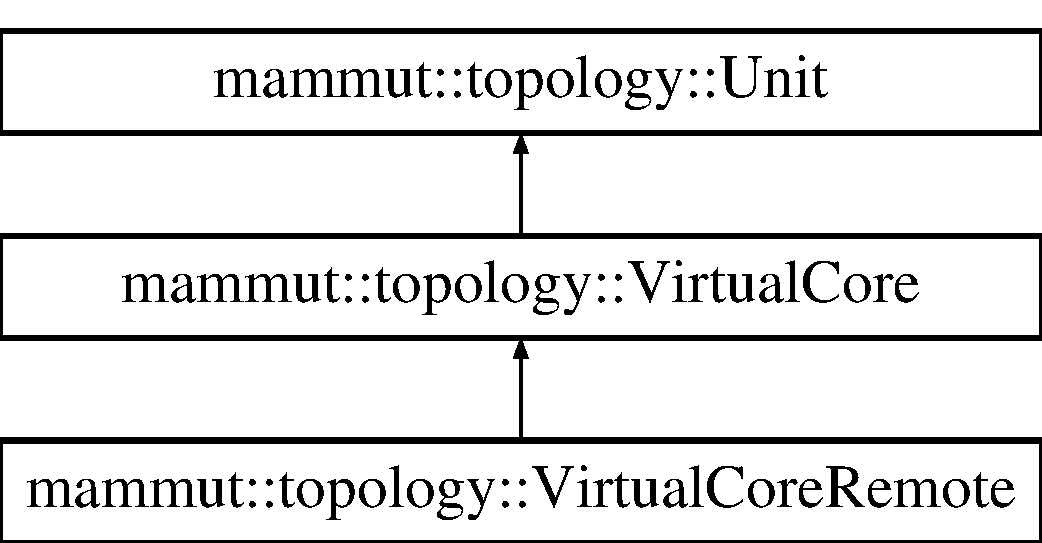
\includegraphics[height=3.000000cm]{classmammut_1_1topology_1_1VirtualCoreRemote}
\end{center}
\end{figure}
\subsection*{Public Member Functions}
\begin{DoxyCompactItemize}
\item 
\hypertarget{classmammut_1_1topology_1_1VirtualCoreRemote_a60d99247cb0af8fef314068d22e2e8fa}{{\bfseries Virtual\-Core\-Remote} (\hyperlink{classmammut_1_1Communicator}{Communicator} $\ast$const communicator, Cpu\-Id cpu\-Id, Physical\-Core\-Id physical\-Core\-Id, Virtual\-Core\-Id virtual\-Core\-Id)}\label{classmammut_1_1topology_1_1VirtualCoreRemote_a60d99247cb0af8fef314068d22e2e8fa}

\item 
bool \hyperlink{classmammut_1_1topology_1_1VirtualCoreRemote_a0968fac0f22747b5663741673225999e}{has\-Flag} (const std\-::string \&flag\-Name) const 
\item 
uint64\-\_\-t \hyperlink{classmammut_1_1topology_1_1VirtualCoreRemote_a2f5a7e3738b84dd04436167eb7ef2f75}{get\-Absolute\-Ticks} () const 
\item 
void \hyperlink{classmammut_1_1topology_1_1VirtualCoreRemote_abc026a4e9ae7db3c0d8373c520b4312d}{maximize\-Utilization} () const 
\item 
void \hyperlink{classmammut_1_1topology_1_1VirtualCoreRemote_a43ea3102cdebec0ce6991b5638e3c4e2}{reset\-Utilization} () const 
\item 
double \hyperlink{classmammut_1_1topology_1_1VirtualCoreRemote_a839fc0934e9aa994deb5538829299ed6}{get\-Idle\-Time} () const 
\item 
void \hyperlink{classmammut_1_1topology_1_1VirtualCoreRemote_a9319506b3bb0e2e457fd6f8c3376efa9}{reset\-Idle\-Time} ()
\item 
bool \hyperlink{classmammut_1_1topology_1_1VirtualCoreRemote_a8675d2a4fc13d470e427f1e3a55d41c8}{is\-Hot\-Pluggable} () const 
\item 
bool \hyperlink{classmammut_1_1topology_1_1VirtualCoreRemote_a8242f18df08037f47886ecc42c0b451b}{is\-Hot\-Plugged} () const 
\item 
void \hyperlink{classmammut_1_1topology_1_1VirtualCoreRemote_a763728a004cb02e6263232ddda0b77b4}{hot\-Plug} () const 
\item 
void \hyperlink{classmammut_1_1topology_1_1VirtualCoreRemote_a0a6a44ac33ecdaeb00fc28f0f2a568a9}{hot\-Unplug} () const 
\item 
std\-::vector\\*
$<$ \hyperlink{classmammut_1_1topology_1_1VirtualCoreIdleLevel}{Virtual\-Core\-Idle\-Level} $\ast$ $>$ \hyperlink{classmammut_1_1topology_1_1VirtualCoreRemote_aaad295d5f06de21eaaff941e840de3df}{get\-Idle\-Levels} () const 
\end{DoxyCompactItemize}
\subsection*{Additional Inherited Members}


\subsection{Member Function Documentation}
\hypertarget{classmammut_1_1topology_1_1VirtualCoreRemote_a2f5a7e3738b84dd04436167eb7ef2f75}{\index{mammut\-::topology\-::\-Virtual\-Core\-Remote@{mammut\-::topology\-::\-Virtual\-Core\-Remote}!get\-Absolute\-Ticks@{get\-Absolute\-Ticks}}
\index{get\-Absolute\-Ticks@{get\-Absolute\-Ticks}!mammut::topology::VirtualCoreRemote@{mammut\-::topology\-::\-Virtual\-Core\-Remote}}
\subsubsection[{get\-Absolute\-Ticks}]{\setlength{\rightskip}{0pt plus 5cm}uint64\-\_\-t mammut\-::topology\-::\-Virtual\-Core\-Remote\-::get\-Absolute\-Ticks (
\begin{DoxyParamCaption}
{}
\end{DoxyParamCaption}
) const\hspace{0.3cm}{\ttfamily [virtual]}}}\label{classmammut_1_1topology_1_1VirtualCoreRemote_a2f5a7e3738b84dd04436167eb7ef2f75}
Gets the clock ticks of this virtual core. \begin{DoxyReturn}{Returns}
The clock ticks of this virtual core. If 0 is returned, ticks are not available. A\-T\-T\-E\-N\-T\-I\-O\-N\-: In general, ticks may change with frequency, i.\-e. the amount of ticks per second at 1\-G\-Hz may be different from the amount of ticks per second at 2\-G\-Hz. To check if ticks do not change with the frequency, you should use '\hyperlink{classmammut_1_1topology_1_1VirtualCore_a82bf6ba883ee5bdc4ef4b3c0fb300207}{are\-Ticks\-Constant()}' call. 
\end{DoxyReturn}


Implements \hyperlink{classmammut_1_1topology_1_1VirtualCore_a0b1ac9c138d1ed5e8eceb38e619e1e65}{mammut\-::topology\-::\-Virtual\-Core}.

\hypertarget{classmammut_1_1topology_1_1VirtualCoreRemote_aaad295d5f06de21eaaff941e840de3df}{\index{mammut\-::topology\-::\-Virtual\-Core\-Remote@{mammut\-::topology\-::\-Virtual\-Core\-Remote}!get\-Idle\-Levels@{get\-Idle\-Levels}}
\index{get\-Idle\-Levels@{get\-Idle\-Levels}!mammut::topology::VirtualCoreRemote@{mammut\-::topology\-::\-Virtual\-Core\-Remote}}
\subsubsection[{get\-Idle\-Levels}]{\setlength{\rightskip}{0pt plus 5cm}std\-::vector$<${\bf Virtual\-Core\-Idle\-Level}$\ast$$>$ mammut\-::topology\-::\-Virtual\-Core\-Remote\-::get\-Idle\-Levels (
\begin{DoxyParamCaption}
{}
\end{DoxyParamCaption}
) const\hspace{0.3cm}{\ttfamily [virtual]}}}\label{classmammut_1_1topology_1_1VirtualCoreRemote_aaad295d5f06de21eaaff941e840de3df}
Returns the idle levels (C-\/\-States) supported by this virtual core. \begin{DoxyReturn}{Returns}
The idle levels supported by this virtual core. If the vector is empty, no idle levels are supported. 
\end{DoxyReturn}


Implements \hyperlink{classmammut_1_1topology_1_1VirtualCore_a841dd64b1b74b28a0533cc1aa9d8cb84}{mammut\-::topology\-::\-Virtual\-Core}.

\hypertarget{classmammut_1_1topology_1_1VirtualCoreRemote_a839fc0934e9aa994deb5538829299ed6}{\index{mammut\-::topology\-::\-Virtual\-Core\-Remote@{mammut\-::topology\-::\-Virtual\-Core\-Remote}!get\-Idle\-Time@{get\-Idle\-Time}}
\index{get\-Idle\-Time@{get\-Idle\-Time}!mammut::topology::VirtualCoreRemote@{mammut\-::topology\-::\-Virtual\-Core\-Remote}}
\subsubsection[{get\-Idle\-Time}]{\setlength{\rightskip}{0pt plus 5cm}double mammut\-::topology\-::\-Virtual\-Core\-Remote\-::get\-Idle\-Time (
\begin{DoxyParamCaption}
{}
\end{DoxyParamCaption}
) const\hspace{0.3cm}{\ttfamily [virtual]}}}\label{classmammut_1_1topology_1_1VirtualCoreRemote_a839fc0934e9aa994deb5538829299ed6}
Returns the number of microseconds that this virtual core have been idle since the last call of \hyperlink{classmammut_1_1topology_1_1VirtualCoreRemote_a9319506b3bb0e2e457fd6f8c3376efa9}{reset\-Idle\-Time()} (or since the creation of this virtual core handler). \begin{DoxyReturn}{Returns}
The number of microseconds that this virtual core have been idle. 
\end{DoxyReturn}


Implements \hyperlink{classmammut_1_1topology_1_1VirtualCore_ad4a33cf2323e7b05537485e4b08a4f12}{mammut\-::topology\-::\-Virtual\-Core}.

\hypertarget{classmammut_1_1topology_1_1VirtualCoreRemote_a0968fac0f22747b5663741673225999e}{\index{mammut\-::topology\-::\-Virtual\-Core\-Remote@{mammut\-::topology\-::\-Virtual\-Core\-Remote}!has\-Flag@{has\-Flag}}
\index{has\-Flag@{has\-Flag}!mammut::topology::VirtualCoreRemote@{mammut\-::topology\-::\-Virtual\-Core\-Remote}}
\subsubsection[{has\-Flag}]{\setlength{\rightskip}{0pt plus 5cm}bool mammut\-::topology\-::\-Virtual\-Core\-Remote\-::has\-Flag (
\begin{DoxyParamCaption}
\item[{const std\-::string \&}]{flag\-Name}
\end{DoxyParamCaption}
) const\hspace{0.3cm}{\ttfamily [virtual]}}}\label{classmammut_1_1topology_1_1VirtualCoreRemote_a0968fac0f22747b5663741673225999e}
Checks if this virtual core has a specific flag 

Implements \hyperlink{classmammut_1_1topology_1_1VirtualCore_aa9f4400708c97197f66bcd11aa0eb990}{mammut\-::topology\-::\-Virtual\-Core}.

\hypertarget{classmammut_1_1topology_1_1VirtualCoreRemote_a763728a004cb02e6263232ddda0b77b4}{\index{mammut\-::topology\-::\-Virtual\-Core\-Remote@{mammut\-::topology\-::\-Virtual\-Core\-Remote}!hot\-Plug@{hot\-Plug}}
\index{hot\-Plug@{hot\-Plug}!mammut::topology::VirtualCoreRemote@{mammut\-::topology\-::\-Virtual\-Core\-Remote}}
\subsubsection[{hot\-Plug}]{\setlength{\rightskip}{0pt plus 5cm}void mammut\-::topology\-::\-Virtual\-Core\-Remote\-::hot\-Plug (
\begin{DoxyParamCaption}
{}
\end{DoxyParamCaption}
) const\hspace{0.3cm}{\ttfamily [virtual]}}}\label{classmammut_1_1topology_1_1VirtualCoreRemote_a763728a004cb02e6263232ddda0b77b4}
Hotplugs this virtual core. If this core is not hot-\/pluggable, nothing is done. 

Implements \hyperlink{classmammut_1_1topology_1_1VirtualCore_a7674d352e60bb8d9c183ca54f62b383d}{mammut\-::topology\-::\-Virtual\-Core}.

\hypertarget{classmammut_1_1topology_1_1VirtualCoreRemote_a0a6a44ac33ecdaeb00fc28f0f2a568a9}{\index{mammut\-::topology\-::\-Virtual\-Core\-Remote@{mammut\-::topology\-::\-Virtual\-Core\-Remote}!hot\-Unplug@{hot\-Unplug}}
\index{hot\-Unplug@{hot\-Unplug}!mammut::topology::VirtualCoreRemote@{mammut\-::topology\-::\-Virtual\-Core\-Remote}}
\subsubsection[{hot\-Unplug}]{\setlength{\rightskip}{0pt plus 5cm}void mammut\-::topology\-::\-Virtual\-Core\-Remote\-::hot\-Unplug (
\begin{DoxyParamCaption}
{}
\end{DoxyParamCaption}
) const\hspace{0.3cm}{\ttfamily [virtual]}}}\label{classmammut_1_1topology_1_1VirtualCoreRemote_a0a6a44ac33ecdaeb00fc28f0f2a568a9}
Hotunplugs this virtual core. If this core is not hot-\/pluggable, nothing is done. 

Implements \hyperlink{classmammut_1_1topology_1_1VirtualCore_a1e8ce49fd0885331533fa85ad7504a9d}{mammut\-::topology\-::\-Virtual\-Core}.

\hypertarget{classmammut_1_1topology_1_1VirtualCoreRemote_a8675d2a4fc13d470e427f1e3a55d41c8}{\index{mammut\-::topology\-::\-Virtual\-Core\-Remote@{mammut\-::topology\-::\-Virtual\-Core\-Remote}!is\-Hot\-Pluggable@{is\-Hot\-Pluggable}}
\index{is\-Hot\-Pluggable@{is\-Hot\-Pluggable}!mammut::topology::VirtualCoreRemote@{mammut\-::topology\-::\-Virtual\-Core\-Remote}}
\subsubsection[{is\-Hot\-Pluggable}]{\setlength{\rightskip}{0pt plus 5cm}bool mammut\-::topology\-::\-Virtual\-Core\-Remote\-::is\-Hot\-Pluggable (
\begin{DoxyParamCaption}
{}
\end{DoxyParamCaption}
) const\hspace{0.3cm}{\ttfamily [virtual]}}}\label{classmammut_1_1topology_1_1VirtualCoreRemote_a8675d2a4fc13d470e427f1e3a55d41c8}
Returns true if this virtual core is hot-\/pluggable. \begin{DoxyReturn}{Returns}
True if this virtual core is hot-\/pluggable, false otherwise. 
\end{DoxyReturn}


Implements \hyperlink{classmammut_1_1topology_1_1VirtualCore_ab8eb88bee673244367a5394de87142d5}{mammut\-::topology\-::\-Virtual\-Core}.

\hypertarget{classmammut_1_1topology_1_1VirtualCoreRemote_a8242f18df08037f47886ecc42c0b451b}{\index{mammut\-::topology\-::\-Virtual\-Core\-Remote@{mammut\-::topology\-::\-Virtual\-Core\-Remote}!is\-Hot\-Plugged@{is\-Hot\-Plugged}}
\index{is\-Hot\-Plugged@{is\-Hot\-Plugged}!mammut::topology::VirtualCoreRemote@{mammut\-::topology\-::\-Virtual\-Core\-Remote}}
\subsubsection[{is\-Hot\-Plugged}]{\setlength{\rightskip}{0pt plus 5cm}bool mammut\-::topology\-::\-Virtual\-Core\-Remote\-::is\-Hot\-Plugged (
\begin{DoxyParamCaption}
{}
\end{DoxyParamCaption}
) const\hspace{0.3cm}{\ttfamily [virtual]}}}\label{classmammut_1_1topology_1_1VirtualCoreRemote_a8242f18df08037f47886ecc42c0b451b}
Returns true if this virtual core is hot plugged. \begin{DoxyReturn}{Returns}
True if this virtual core is hot plugged or if hotplug is not supported, false otherwise. 
\end{DoxyReturn}


Implements \hyperlink{classmammut_1_1topology_1_1VirtualCore_a61bd18dbc9bd35f6b22e9bbd7947427d}{mammut\-::topology\-::\-Virtual\-Core}.

\hypertarget{classmammut_1_1topology_1_1VirtualCoreRemote_abc026a4e9ae7db3c0d8373c520b4312d}{\index{mammut\-::topology\-::\-Virtual\-Core\-Remote@{mammut\-::topology\-::\-Virtual\-Core\-Remote}!maximize\-Utilization@{maximize\-Utilization}}
\index{maximize\-Utilization@{maximize\-Utilization}!mammut::topology::VirtualCoreRemote@{mammut\-::topology\-::\-Virtual\-Core\-Remote}}
\subsubsection[{maximize\-Utilization}]{\setlength{\rightskip}{0pt plus 5cm}void mammut\-::topology\-::\-Virtual\-Core\-Remote\-::maximize\-Utilization (
\begin{DoxyParamCaption}
{}
\end{DoxyParamCaption}
) const\hspace{0.3cm}{\ttfamily [virtual]}}}\label{classmammut_1_1topology_1_1VirtualCoreRemote_abc026a4e9ae7db3c0d8373c520b4312d}
Bring the utilization of this virtual core to 100\% until \hyperlink{classmammut_1_1topology_1_1VirtualCoreRemote_a43ea3102cdebec0ce6991b5638e3c4e2}{reset\-Utilization()} is called. 

Implements \hyperlink{classmammut_1_1topology_1_1VirtualCore_ac4e3a17bc401689c387f27a90e24daf5}{mammut\-::topology\-::\-Virtual\-Core}.

\hypertarget{classmammut_1_1topology_1_1VirtualCoreRemote_a9319506b3bb0e2e457fd6f8c3376efa9}{\index{mammut\-::topology\-::\-Virtual\-Core\-Remote@{mammut\-::topology\-::\-Virtual\-Core\-Remote}!reset\-Idle\-Time@{reset\-Idle\-Time}}
\index{reset\-Idle\-Time@{reset\-Idle\-Time}!mammut::topology::VirtualCoreRemote@{mammut\-::topology\-::\-Virtual\-Core\-Remote}}
\subsubsection[{reset\-Idle\-Time}]{\setlength{\rightskip}{0pt plus 5cm}void mammut\-::topology\-::\-Virtual\-Core\-Remote\-::reset\-Idle\-Time (
\begin{DoxyParamCaption}
{}
\end{DoxyParamCaption}
)\hspace{0.3cm}{\ttfamily [virtual]}}}\label{classmammut_1_1topology_1_1VirtualCoreRemote_a9319506b3bb0e2e457fd6f8c3376efa9}
Resets the number of microseconds that this virtual core have been idle 

Implements \hyperlink{classmammut_1_1topology_1_1VirtualCore_a8fc6a3a4882ca369e37a3a9f0f668d9c}{mammut\-::topology\-::\-Virtual\-Core}.

\hypertarget{classmammut_1_1topology_1_1VirtualCoreRemote_a43ea3102cdebec0ce6991b5638e3c4e2}{\index{mammut\-::topology\-::\-Virtual\-Core\-Remote@{mammut\-::topology\-::\-Virtual\-Core\-Remote}!reset\-Utilization@{reset\-Utilization}}
\index{reset\-Utilization@{reset\-Utilization}!mammut::topology::VirtualCoreRemote@{mammut\-::topology\-::\-Virtual\-Core\-Remote}}
\subsubsection[{reset\-Utilization}]{\setlength{\rightskip}{0pt plus 5cm}void mammut\-::topology\-::\-Virtual\-Core\-Remote\-::reset\-Utilization (
\begin{DoxyParamCaption}
{}
\end{DoxyParamCaption}
) const\hspace{0.3cm}{\ttfamily [virtual]}}}\label{classmammut_1_1topology_1_1VirtualCoreRemote_a43ea3102cdebec0ce6991b5638e3c4e2}
Resets the utilization of this virtual core. 

Implements \hyperlink{classmammut_1_1topology_1_1VirtualCore_a94374b13113f0294c5178b6fc275ecc0}{mammut\-::topology\-::\-Virtual\-Core}.



The documentation for this class was generated from the following file\-:\begin{DoxyCompactItemize}
\item 
/home/daniele/\-Code/\-Mammut/mammut/topology/topology-\/remote.\-hpp\end{DoxyCompactItemize}

%--- End generated contents ---

% Index
\newpage
\phantomsection
\addcontentsline{toc}{chapter}{Index}
\printindex

\end{document}
